\documentclass[]{nrel}
% Document metadata: the one place to update when a new release is documented.
% main.tex reads these for the title page and the PDF properties.
\newcommand{\ReportTitle}{ComStock Reference Documentation}
\newcommand{\ReportRelease}{2025 Release 3}
\newcommand{\ReportAuthors}{\mbox{Andrew Parker}, \mbox{Henry Horsey}, \mbox{Matthew Dahlhausen}, \mbox{Marlena Praprost}, \mbox{Christopher CaraDonna}, \mbox{Amy Van Sant}, \mbox{Janghyun Kim}, \mbox{Lauren Klun}, \mbox{Eric Ringold}, \mbox{Wenyi Kuang}, and \mbox{Landan Taylor}}
\newcommand{\ReportPdfAuthor}{Andrew Parker and others}
\newcommand{\ReportAffiliation}{National Renewable Energy Laboratory}

\usepackage{multirow}
\usepackage{longtable}
\usepackage{float}
\usepackage[section]{placeins}
\usepackage{pdflscape}
\usepackage{soul}
\usepackage{threeparttable}
\usepackage{bookmark}

\hypersetup{
    colorlinks=true,
    linkcolor=black,
    citecolor=blue,
    urlcolor=blue,
    bookmarks=true,
    bookmarksnumbered=true,
    bookmarksopen=true,
    bookmarksopenlevel=1,
    pdfstartview=FitH,
    pdftitle={\ReportTitle: \ReportRelease},
    pdfauthor={\ReportPdfAuthor},
    pdfsubject={ComStock Building Energy Modeling},
    pdfkeywords={ComStock; Building Energy; Commercial Buildings; Energy Modeling}
}
\usepackage{cleveref}

% Fix frontmatter TOC indentation
\makeatletter
\let\oldfrontmatter\frontmatter
\renewcommand{\frontmatter}{%
    \oldfrontmatter
    \addtocontents{toc}{\protect\setlength{\protect\cftchapnumwidth}{0pt}}
}
\let\oldmainmatter\mainmatter
\renewcommand{\mainmatter}{%
    \addtocontents{toc}{\protect\setlength{\protect\cftchapnumwidth}{1.5em}}
    \oldmainmatter
}
\makeatother

% -----------------------------------
% DOCUMENT PROPERTIES
% -----------------------------------
\title{\ReportTitle:\\[0.3em] \ReportRelease}

\author{\ReportAuthors}
\affil{\ReportAffiliation}

\fancypagestyle{plain}{}
\addbibresource{bibliography.bib}
\setcounter{tocdepth}{2}

% -------------------------------------
% DOCUMENT STARTS HERE
% -------------------------------------
\begin{document}
\frontmatter

\tableofcontents

\include{0_1_exec_summary}
\include{0_2_acknowledgements}
\chapter*{List of Acronyms}
\addcontentsline{toc}{chapter}{List of Acronyms}
\begin{acronym}[EJSCREEN]
    \acro{AAMA}{American Architectural Manufacturers Association}
    \acro  {AC}   {air conditioner or air conditioning}
    \acro  {ACC}   {air-cooled chiller}
    \acro{ADA}{Americans with Disabilities Act}
    \acro{AER}{average emissions rate}
    \acro{AFUE}{annual fuel utilization efficiency}
    \acro{AHA}{American Hospital Association}
    \acro  {AHU}  {air handling unit}
    \acro{AMI}{Advanced Metering Infrastructure}
    \acro{AMY}{actual meteorological year}
    \acro  {ASHP}  {air-source heat pump}
    \acro{ASHRAE}{American Society of Heating, Refrigerating and Air-Conditioning Engineers}
    \acro{AWS}{Amazon Web Services}
    \acro{BA}{balancing authority}
    \acro  {BAS}  {building automation system}
    \acro{BEM}{building energy model}
    \acro{BPR}{base-to-peak ratio}
    \acro{BTU}{British thermal unit}
    \acro{CAEUS}{California End Use Survey}
    \acro{CAPFT}{capacity as a function of temperature}
    \acro  {CBECS} {Commercial Buildings Energy Consumption Survey}
    \acro{CBSA}{Commercial Building Stock Assessment}
    \acro{CEC}{California Energy Commission}
    \acro{CEJST}{Climate and Economic Justice Screening Tool}
    \acro{CFL}{compact fluorescent light}
    \acro{cfm}{cubic feet per minute}
    \acro  {CHW} {chilled water}
    \acro{CMU}{concrete masonry unit}
    \acro  {COP}  {coefficient of performance}
    \acro{CPUC}{California Public Utilities Commission}
    \acro{CU}{coefficient of utilization}
    \acro  {CW} {condenser water}
    \acro{CZ} {climate zone}
    \acro  {DCV} {demand control ventilation}
    \acro{DEER}{Database of Energy Efficiency Resources}
    \acro{DOAS}{dedicated outdoor air system}
    \acro  {DOE}  {U.S. Department of Energy}
    \acro{DST}{daylight saving time}
    \acro  {DX}  {direct expansion}
    \acro{EER}{energy efficiency ratio}
    \acro{EFFFPLR}{efficiency function of part load ratio}
    \acro  {EIA} {U.S. Energy Information Administration}
    \acro  {EIR} {energy input ratio}
    \acro{EIRFPLR}{energy input ratio as a function of part load ratio}
    \acro{EIRFT}{energy input ratio as a function of temperature}
    \acro{EJSCREEN}{Environmental Justice Screening and Mapping Tool}
    \acro{EMS}{energy management system}
    \acro{EPA}{U.S. Environmental Protection Agency}
    \acro  {EPD}  {equipment power density}
    \acro  {ERV}  {energy recovery ventilator}
    \acro{EST}{Eastern Standard Time}
    \acro  {EUI}  {energy use intensity}
    \acro{EUL}{effective useful life}
    \acro{EULP}{end-use load profiles}
    \acro{FIPS}{Federal Information Processing Standard}
    \acro{GGHC}{Green Guide for Healthcare}
    \acro{gpm}{gallons per minute}
    \acro  {GSHP}  {ground-source heat pump}
    \acro{HID}{high intensity discharge}
    \acro{HIFLD}{Homeland Infrastructure Foundation-Level Data}
    \acro{HP}{horse power}
    \acro  {HSIP} {Homeland Security Infrastructure Program}
    \acro{HSPF}{heating seasonal performance factor}
    \acro  {HVAC} {heating, ventilating, and air conditioning}
    \acro  {HW} {hot water}
    \acro {IEAD} {insulation entirely above deck}
    \acro{IEEE}{Institute of Electrical and Electronics Engineers}
    \acro  {ISO}  {independent system operator}
    \acro{IT}{information technology}
    \acro{LBNL}{Lawrence Berkeley National Laboratory}
    \acro{LDD}{luminaire dirt depreciation}
    \acro{LED}{light-emitting diode}
    \acro{LFF}{lighting loss factor}
    \acro{LLD}{lamp lumen depreciation}
    \acro{LMC}{lighting market characterization}
    \acro  {LPD}  {lighting power density}
    \acro{LRMER}{long-run marginal emission rate}
    \acro {LSM} {lighting subcommittee model}
    \acro{NEEA}{Northwest Energy Efficiency Alliance}
    \acro  {NEMS} {National Energy Modeling System}
    \acro{NFRC}{National Fenestration Rating Council}
    \acro{NHGIS}{National Historical Geographic Information System}
    \acro  {NREL} {National Renewable Energy Laboratory}
    \acro{OEDI}{Open Energy Data Initiative}
    \acro  {PADD} {Petroleum Administration for Defense District}
    \acro  {PFP} {parallel fan-powered}
    \acro {PJM} {Pennsylvania-New Jersey-Maryland Interconnection}
    \acro  {PLR} {part load ratio}
    \acro{PPL}{plug and process load}
    \acro{PNNL}{Pacific Northwest National Laboratory}
    \acro  {PSZ-AC} {packaged single-zone air conditioner}
    \acro  {PSZ-HP} {packaged single-zone heat pump}
    \acro  {PTAC} {packaged terminal air conditioner}
    \acro  {PTHP} {packaged terminal heat pump}
    \acro  {PVAV} {packaged variable air volume}
    \acro  {PPL}  {plug and process loads}
    \acro  {PUMA} {Public Use Microdata Area}
    \acro{RECS}{Residential Energy Consumption Survey}
    \acro{ReEDS}{Regional Energy Deployment System}
    \acro{RSDD}{room surface dirt depreciation}
    \acro{RTO}{regional transmission organization}
    \acro{RTU}{rooftop unit}
    \acro{SEER}{seasonal energy efficiency ratio}
    \acro {SHGC} {solar heat gain coefficient}
    \acro{SSL}{solid state lighting}
    \acro  {SWH}  {service water heating}
    \acro{TF}{total lighting factor}
    \acro{TMY3}{typical meteorological year}
    \acro{Tstat}{thermostat}
    \acro{UTC}{Coordinated Universal Time}
    \acro{URDB}{Utility Rate Database}
    \acro  {VAV}  {variable air volume}
    \acro{VLT}{visible light transmittance}
    \acro{VRF}{variable refrigerant flow}
    \acro  {WCC}   {water-cooled chiller}
    \acro  {WSHP} {water-source heat pump}
    \acro{WWR}{window-to-wall ratio}
\end{acronym}


\listoffigures

\listoftables

\mainmatter
\bookmarksetup{startatroot}
% Chapters and large sections are broken out in separate .tex files to make edits easier
\include{1_introduction}
\chapter{ComStock Workflow}

Accurately representing commercial building energy usage is complex because of how subsystems of a building interact with one another and with the surrounding environment. Every aspect of a commercial building can influence its energy consumption, so it is difficult to identify which aspects of a building are critical for a given energy-related metric and climate without simulation. To achieve its fundamental goal of representing the U.S. commercial building stock across all energy-related metrics, ComStock must capture the diversity and variability of the building stock. This requires a robust modeling and publishing workflow. 

At the heart of ComStock are the approximately 350,000 building energy models (BEMs) that collectively represent the commercial building stock in the United States (roughly 6 million buildings). These models do not represent specific individual buildings (for example, there is no ComStock model for the Empire State Building). Modeling individual buildings would be impractical given the difficulty of compiling accurate data on the U.S. building stock at a national scale. Identifying distributions of characteristics is a more tractable problem. For example, the EIA's Commercial Buildings Energy Consumption Survey (CBECS) \citep{eia2012cbecs} provides information on how many buildings by type have specific heating, ventilating, and air-conditioning (HVAC) system characteristics (e.g., an office building with a chiller). Combining this information with a building's size and when and where it was built has allowed the ComStock team to develop statistical distributions that determine the characteristics for each of the 350,000 models.

Creating and running the 350,000 BEMs that lie at the heart of ComStock---and then sharing the results---requires significant infrastructure. The workflow that defines, executes, and post-processes these BEMs is shown in Figure \ref{fig:comstock_workflow}. The remainder of this section contains an abridged discussion of the elements of this workflow and their role in creating the ComStock BEMs and the results data set. Each aspect of the workflow is revisited in detail in Section 4 as modeling assumptions and algorithms are discussed.

\begin{figure}[h!]
  \centering
  \includegraphics[width=\textwidth]{figures/comstock_workflow.png}
  \caption[Flowchart of the ComStock workflow]{Flowchart of the ComStock workflow.}
  \label{fig:comstock_workflow}
\end{figure}

\pagebreak

ComStock accomplishes its goal of accurately representing the U.S. building stock through a three-part workflow process: \begin{enumerate}
    \item ComStock creates samples that represent the U.S. commercial building stock.
    \item These samples are translated into BEMs and modified to represent either the baseline U.S. commercial building stock or an altered version thereof (i.e., modeling the impact of an efficiency or electrification measure).
    \item The physics-based BEMs are evaluated through an energy simulation engine that uses high-performance computing to simulate each model. The resulting data are made available to a wide range of stakeholders.
\end{enumerate}

\section{ComStock Sample Definitions}
\label{sec:sample_definitions}

ComStock uses a number of publicly and privately available databases that define what buildings exist, where they are located, when they were built, and with what characteristics they have. The characteristics include (but are not limited to) floor area, HVAC system type, and window type, as well as building-type-specific characteristics such as number of beds (for hospitals) or number of students (for educational institutions). When assembled, these data sets provide the basis for representing the U.S. commercial building stock.

The input data sets used to develop ComStock are often the result of extensive, highly capital-intensive data collection efforts. Some of the data sets purchased for this work are subject to data retention clauses that require deletion of the raw data after the contractual use has been completed. Given these contractual agreements, ComStock typically aggregates and joins with other data sets to generate distributional estimates of relationships between key characteristics. These input distributions are the first step in generating samples for ComStock.

Translating the input distributions into individual samples, or combinations of characteristics, requires a sampling process. Currently, ComStock assembles all input distributions as an $n$-dimensional joint probability distribution, which is then sampled using a space-filling sampling algorithm. The goal of the sampling algorithm is to minimize the largest void, or ``gap,'' between individual samples.

Each sample generated by the sampling algorithm defines the input characteristics for a single BEM. This results in hundreds of thousands of BEMs (millions when alterations to the building stock are also considered). Each of these BEMs must be created through automated model-generation scripts (discussed in Section~\ref{sec:openstudio_standards}) and evaluated via a BEM physics engine (discussed in Section~\ref{sec:buildstockbatch}). Additionally, it is often necessary to consider the impact of alterations or retrofits to the building stock---the development and use of Measures are discussed in the following section (Section~\ref{sec:measures}).

\section{Measures for ComStock}
\label{sec:measures}

A major advantage of physics-based models is their ability to change the inputs and evaluate the effect on the outputs. For ComStock, such changes are primarily evaluated using Energy Efficiency Measures or Electrification Measures. Although the word \emph{measure} has a generally accepted meaning in the energy efficiency industry, when capitalized henceforth, \emph{Measure} indicates a script that can be executed on the ComStock BEMs to alter the model inputs. A collection of Measures is a collection of scripts that allow various alterations---such as energy efficiency interventions, electrification interventions, or demand-response strategies/technologies---to be applied across the 350,000 BEMs that comprise a national run with ComStock. These automated alterations are a key aspect of ComStock's value proposition.

Throughout ComStock's development, various Measures have been developed for specific projects. These include Measures developed to support the Los Angeles 100\% Renewable Energy Study (LA100), the Advanced Building Construction Typology Report, and, in ComStock's infancy, the Electrification Futures Study. Currently, the ComStock team is developing a more robust and generalized set of Measures that will be published. These Measures are still in development, but at minimum will include efficiency and electrification Measures.

A key element of Measures is the interconnected nature of the intervention and the BEM representation of building systems and technologies. As an example, when modeling an intervention that adds an economizer to all rooftop units without an economizer, the modeling workflow relies on (a) the Measure identifying which rooftop units already have an economizer, and (b) the Measure updating the BEMs that do not have an economizer.

In the case of a Measure that electrifies forklifts in warehouses, however, two issues arise. First, none of ComStock's sample definition characteristics provide information on which warehouses (or other building types) this measure is applicable to, or to what degree. Second, there is no disambiguation of forklift load vs. other internal load in ComStock. As such, any Measure that attempts to implement this intervention has to rely on scaled measurement and verification or market research studies. In both cases, the estimates may be accurate, but it is difficult to tie the impact to any fundamental characteristic of the model and represent the variability of the impact across buildings. Although this does not invalidate the value of such a measure, it is important to differentiate measures that fit into ComStock's sample definitions and OpenStudio-Standards' workflow from those that are ``bolted on'' post-hoc.

\section{ComStock-Typical and OpenStudio-Standards}
\label{sec:openstudio_standards}

OpenStudio-Standards is an open-source modeling library that defines the detailed inputs of a BEM based on simple input values. It carries two kinds of data. Standards data is vintage-specific: the minimum efficiency of a packaged unit, the maximum lighting power allowance for an office, and the required roof insulation in a climate zone are exactly what changes with the energy code in force when a building system was installed. Typical data describes how buildings are used: how many people occupy a classroom, how much outdoor air a patient room needs, how much hot water a kitchen draws, and what hours a retail store keeps. These values come from ASHRAE Standards 62.1 and 170, CBECS, and field studies, and they do not depend on vintage. A model of a 1985 building therefore receives 1985 equipment efficiencies and present-day assumptions about how its spaces are used.

ComStock builds its models with ComStock-Typical, a fork of OpenStudio-Standards maintained by the ComStock team. The fork keeps the standards data, the typical-building generation workflow, and the HVAC system library, and sets aside the DOE prototype building generation and ASHRAE 90.1 Appendix G baseline tooling, which are code-determination tools rather than tools for representing buildings that exist. Its central abstraction is the \emph{space type}: a vocabulary of space uses---offices, classrooms, patient rooms, kitchens, warehouse storage, and so on---each of which carries its own occupant density, lighting, plug and process loads, outdoor air requirement, exhaust, water draws, thermostat setpoints, and parametric schedules. A building is described to the library as a \emph{specification}: a mix of space types with floor area ratios, a building form, envelope constructions, and a set of overrides for whatever is specific to that building. The library validates the specification, generates the geometry, and populates the model from the space type data. A ComStock building type is therefore a recipe of space types rather than a fixed prototype, and the loads in a model are keyed on what happens in each space rather than on the building type that contains it. Section~\ref{sec:building_spec} describes the specification and how the sampled building characteristics enter it.

OpenStudio-Standards was originally developed to help automate the process of creating energy code baseline BEMs. This allowed for more consistent creation of baseline models for efficiency incentive programs. Throughout the development and calibration of ComStock, these code-minimum assumptions have been altered to better reflect the building performance seen in measured data sources. In some cases, this has resulted in components being defined on a non-code basis (e.g., LEDs), whereas in other cases, calibration has resulted in alterations to the nominal assumptions in code-minimum definitions. These alterations are discussed in detail in the relevant subsections of Section~\ref{chap:4_modeling}.

OpenStudio-Standards was not originally developed for ComStock and is used for many other purposes. The standards represent the collaborative work of many researchers at Lawrence Berkeley National Laboratory, Pacific Northwest National Laboratory, and Oak Ridge National Laboratory.

\section{ComStock Project}

A ComStock project includes a baseline building stock definition and a selection of Measures. For example, a ComStock project that analyzes the building envelope savings potential for the state of Colorado would include all building samples in Colorado and Measures that capture several efficiency levels for walls, roofs, and windows. The results of this project would identify the energy impacts of bringing Colorado commercial building envelopes up to code and/or above code.

Results for a ComStock project are relative to a fixed point in the lifespan of the building stock. For example, ComStock currently represents the building stock as it looked in 2018. Results assume overnight adoption of changes to the building stock. In reality, large-scale changes to the building stock take many years, and the building stock evolves during that process. If either the baseline building stock characteristics or the measures being considered change significantly, careful consideration of the applicability of results is needed. In many cases, the changes in the point in time and the measures being considered will not significantly change the results. However, in some cases, a rapidly evolving understanding of technology performance and saturation, or increasingly refined questions, will trigger the need for updated or refined analyses. For example, state-of-the-art air-source heat pump characteristics may change rapidly, making results from a ComStock project using older technology assumptions obsolete.

\section{BuildStockBatch}
\label{sec:buildstockbatch}

BuildStockBatch is a software library that executes ComStock and ResStock projects. ResStock is a residential building sector model and shares many workflow components with ComStock.  BuildStockBatch is typically used by NREL researchers on NREL's high-performance computing system, Eagle. However, the ResStock team has developed and demonstrated an Amazon Web Services (AWS)-based workflow that can be used by entities without access to the U.S. Department of Energy's (DOE's) high-performance computing system. BuildStockBatch can run up to tens of millions of simulations for a given ComStock (or ResStock) project. Although the number of simulations in these projects can vary greatly, BuildStockBatch scales by distributing simulations across a number of servers. The number of servers increases in proportion to the number of simulations, ranging from a few servers to hundreds of servers. After each server completes its requested simulations, it pushes the results to a remote file-system-based database.

Currently, BuildStockBatch utilizes an Eagle high-performance computing workflow for ComStock. In the future, ComStock expects to provide a proof-of-concept BuildStockBatch implementation that uses AWS to execute a ComStock simulation. It is not yet clear whether funding will be allocated to support this workflow's use by third-party users, but the AWS-enabled code base will be publicly available when developed.

\section{Raw Simulation Results}
\label{rawsimulationresults}
The simulation results from national ComStock releases are transferred to an AWS bucket provided by the Open Energy Data Initiative (OEDI) Data Lake partnership with AWS. This bucket contains several versions of the raw results. It contains the OpenStudio BEMs (.osm files) used to represent each sampled building. It also provides each building sample's simulated energy consumption results on a 15-minute basis, per end use, per Measure upgrade. These files are stored such that they can be queried using AWS's Athena service. Finally, the annualized results are provided on a baseline/upgrade basis, where each Measure upgrade defined in the ComStock project has its own annualized result file.

\section{Web-Based Visualization Platform}
\label{dataviewer}
ComStock and ResStock utilize a shared platform for data visualization. In most cases, users are looking for the sum or average load profile of all buildings of a given type in a given geographic area. These are referred to as ``aggregate'' load profiles. The visualization platform, which can be found at \href{comstock.nrel.gov}{comstock.nrel.gov}, provides users with an interface to interact with both annualized and 15-minute-interval data segmented by geography and building characteristic. As previously discussed, ComStock does not providet results that represent specific buildings, but rather aims to represent the distribution and variability of the building stock across the United States. Users who interact with \href{comstock.nrel.gov}{comstock.nrel.gov} generally have a more consistent and beneficial experience than those who interact with individual sample results. The results are available for several weather years and several different geographic resolutions. It is important to note that, at present, the more refined the geographic resolution, the less confidence should be placed in the results. This is because fewer samples will have been generated to approximate the relevant stock.
\chapter{Building Characteristic Sampling}

There are three steps to creating the sample of buildings modeled by ComStock. The first step creates estimates of the sizes, ages, types, and locations of the buildings that exist throughout the United States. The second step is characteristic estimation, which is detailed in Section~\ref{chap:4_modeling}. This step defines the additional characteristics of buildings that determine energy consumption and performance. These characteristics are mostly derived from different data sources than those used in the stock estimation step, although they often depend on stock estimation parameters such as building type or age. The third step is sampling the multidimensional probability space to generate a collection of input parameters, or samples. The final samples give an accurate estimation of the commercial building stock at large while not attempting to model any individual building exactly. Stock estimation and sampling are described further in this section, but the majority of the characteristics are discussed in Section~\ref{chap:4_modeling}.

\section{Stock Estimation}

Any estimate of the energy consumption of the U.S. commercial building stock relies heavily on an estimate of how much floor area of each type of building exists in each part of the country. As shown by CBECS \citep{eia2018cbecs} and others, energy consumption of commercial buildings predominantly scales with floor area, not with building count. An accurate estimate of building floor area is therefore a critical input into any stock modeling tool focused on energy or energy-related metrics.

A secondary issue is the type of building associated with each floor area. Although accurately estimating the total floor area of commercial buildings is necessary, it is not sufficient, as building type also has an impact on energy use intensity (EUI), measured in units of energy use per square foot per year. As an example, a large office with a data center would be expected to have a dramatically higher electric load per square foot than an unconditioned warehouse.

The goal of the stock estimation process is to identify the type, floor area, and location of buildings across the United States. This task is complicated by a number of factors, including data sources that are inconsistent across the United States. However, floor area estimation is central to ensuring that ComStock is accurate for its intended use cases. ComStock takes a three step approach towards achieving an accurate estimate. To begin, national data sources are assembled to present overlapping (and often conflicting) reports of the U.S. commercial building stock. Second, the buildings reported by the various data sources are assigned a consistent set of type descriptors---e.g., large office or secondary school. Finally, the various data sets are amalgamated to create a final, consistent data set that is used in the sampling process.

\subsection{Data Sources}\label{sec:data_sources}

ComStock's stock estimation is assembled using several data sources. The primary data sources are CoStar, a commercial building real estate intelligence broker, and Homeland Infrastructure Foundation-Level Data (HIFLD), a Department of Homeland Security database that provides cross-agency information on critical infrastructure assets across the United States. Hospitals come from a third source, the American Hospital Association (AHA) Annual Survey \citep{aha_annual_survey_2022}. These data sets, due to their business-/mission-driven use cases, tend to have very high accuracy for the buildings they represent. However, the major downside of these data sources is that the buildings they do not collect data on are not represented in any manner. While this is challenging, it is easier to adjust/correct for this sparsity than to use other data sets in which buildings are incorrectly and inconsistently represented.

CoStar is a ``leading provider of commercial real estate data and marketplace listing platforms. Its data offerings contain in-depth analytical information on over five million commercial real estate properties related to various subsections, including office, retail, multifamily, healthcare, industrial, self-storage, and data centers'' \citep{costar_10k}. CoStar's data is driven by commercial leases and commercial sales data, and is updated with millions of dollars' worth of research per year. CoStar's data set is not always complete, both in terms of geography and building type. For example, building types that are rarely bought and sold, such as schools and major hospital complexes, are less likely to be represented in CoStar's database.

HIFLD is a set of data tables assembled by the U.S. Department of Homeland Security to support critical infrastructure awareness, disaster recovery, and various other uses. Their databases include information on critical infrastructure facilities such as refineries and military bases, but also include information on schools (which are often used as disaster assistance centers) and hospitals. This is particularly useful, as these are two of the key building types that are less likely to be represented in CoStar. The schools data set provided by HIFLD always provides information on the number of students enrolled in a given school, which is used as a proxy to determine the floor area of the school when not otherwise available. Stock estimates before 2026 R1 also took hospitals from HIFLD. Its hospital table fails to report the number of beds in a given hospital (which was likewise used to scale floor area) in approximately half the states in the United States, and in these cases data from states that do report this information were generalized and used to infer the floor area in states without data. Beginning with the 2026 R1 stock estimate, hospitals come from the AHA Annual Survey instead.

The AHA Annual Survey \citep{aha_annual_survey_2022} reports the number of beds and the gross floor area of each hospital, so hospital floor area no longer has to be inferred from beds, and its coverage is more consistent across the country than that of the HIFLD hospital table. The 2022 survey is corrected in two steps before it is used. First, the floor area that many hospitals report includes space that does not belong to the hospital itself, most notably freestanding outpatient centers and offices. Hospitals are sorted into six categories, using the number of beds as the primary indicator and floor area as a secondary indicator \citep{cms_critical_access_hospitals, definitive_hospital_square_footage}: critical access hospitals (1--25 beds), small community hospitals (26--100 beds), community general acute hospitals (101--250 beds), regional referral hospitals (251--500 beds), academic medical centers (501--1,000 beds), and quaternary academic medical centers (more than 1,000 beds). In every category, two-sample Kolmogorov--Smirnov tests show that hospitals that report a freestanding outpatient center have a different distribution of floor area per bed than hospitals that do not, with more floor area per bed. The floor area per bed of each hospital with an outpatient center is rescaled to match the distribution of the hospitals without one, and the removed area is assigned to a separate outpatient building group rather than to the hospital. Second, some hospitals still report a floor area per bed that is not realistic for their size. These are screened with an adjusted boxplot \citep{hubert2008adjusted}, which sets the fences of each category from the medcouple, a robust measure of skewness, as shown in Equation~\ref{eqn:adjusted_boxplot}.

\begin{align}
\label{eqn:adjusted_boxplot}
\text{fences} =
\begin{cases}
  \left[Q_{1} - 1.5\, e^{-4\,MC}\, IQR,\; Q_{3} + 1.5\, e^{3\,MC}\, IQR\right] & \text{if } MC \geq 0 \\
  \left[Q_{1} - 1.5\, e^{-3\,MC}\, IQR,\; Q_{3} + 1.5\, e^{4\,MC}\, IQR\right] & \text{if } MC < 0
\end{cases}
\end{align}
where:\\
\begin{itemize}
\item \textbf{Q\textsubscript{1}} and \textbf{Q\textsubscript{3}} are the first and third quartiles of floor area per bed in the category\\
\item \textbf{IQR} is the interquartile range, Q\textsubscript{3} $-$ Q\textsubscript{1}\\
\item \textbf{MC} is the medcouple of floor area per bed in the category
\end{itemize}

The fences give a realistic range of floor area per bed for each category. The categories are used only for these corrections; ComStock represents every hospital with its single hospital building type. Each hospital in the 2026 R1 stock estimate carries its own census tract. That estimate holds 5,952 hospitals with 2.10 billion ft$^2$ of floor area in all 50 states and the District of Columbia; the 2025 R3 estimate, built from HIFLD, held 3,224 hospitals with 0.84 billion ft$^2$ in 48 states. As for every building type, ComStock's national hospital floor area is then matched to CBECS, as described next.

Although these data sets provide excellent coverage of buildings they consider, they do not provide full and complete coverage of commercial buildings across the United States. Of particular note, using these data sources results in an estimate of U.S. commercial buildings that differs from that published by CBECS. The ComStock team, after significant discussion, has decided to treat the CBECS estimate of the floor area of each building type as a truth data set. Following the sampling of the CoStar, HIFLD, and AHA data sets, the CBECS estimates are used to ``true up'' the numbers on a national basis. As a result, ComStock's floor area estimates match CBECS' by building type on a national basis. Although other truth data sources were considered, CBECS' centrality to all commercial energy use estimation made it the obvious and consistent choice for estimating the U.S. commercial building stock's energy use.

\subsection{Building Type Assignments} \label{sec:btype_assignments}

Building type definitions frequently do not match across data sources. This is particularly noticeable in the case of CoStar, CBECS, and DOE prototype buildings data sources. The DOE prototype building models, discussed further in Section~\ref{sec:building_type_meta}, defines specific combinations of space types as ``building types,'' which are then used by ComStock. The building types represented by the DOE prototype building models were decided on during the development of their precursors, the DOE reference building models \citep{doe_reference_buildings}. As such, ``translating'' building types across data sources introduces a layer of complexity.

ComStock maps the building type definitions from each data source to a specific building type from the DOE prototype buildings to maximize consistency. While these mappings are imperfect, they represent the best efforts of the ComStock team to capture the unique energy-related characteristics of different building types within the modeling framework created and used by DOE over the last 15 years. Table \ref{tab:building_types} shows the mapping from the CoStar building types, the HIFLD tables, and the AHA Annual Survey to the DOE prototype buildings, and from the DOE prototype buildings to CBECS' Principal Building Activity Plus.

\begin{table}
\centering
\small
\caption[Building Type Mapping Across Data Sources]{Building Type Mapping Across Data Sources}
\label{tab:building_types}
\begin{tabular}{|p{4.25cm}|p{3.5cm}|p{3.25cm}|p{4.25cm}|}
\hline
\textbf{CoStar Building   Type}                                & \multicolumn{1}{l|}{\textbf{HIFLD Table or AHA}}                & \textbf{DOE Prototype and ComStock Building Type}                               & \textbf{CBECS Principle Building Activity Plus }         \\ \hline
Retail:   Bar                                         & \multirow{2}{*}{Not applicable}                 & \multirow{2}{*}{Full service restaurant}  & Restaurant/cafeteria                            \\ \cline{1-1} \cline{4-4}
Retail: Restaurant                                    &                                                 &                                           & Bar/pub/lounge                                  \\ \hline
\multicolumn{1}{|l|}{Not applicable}                  & \multicolumn{1}{l|}{AHA Annual Survey}          & Hospital                                  & Hospital/inpatient health                       \\ \hline
Hospitality: Hotel                                    & \multirow{12}{*}{Not applicable}                & \multirow{2}{*}{Large hotel}              & \multirow{2}{*}{Hotel}                          \\ \cline{1-1}
Hospitality: Hotel casino                             &                                                 &                                           &                                                 \\ \cline{1-1} \cline{3-4}
Office: Industrial live/work   unit                   &                                                 & \multirow{6}{*}{Office}                   & Administrative/professional office              \\ \cline{1-1} \cline{4-4}
Office: Office live/work unit                         &                                                 &                                           & Bank/other financial                            \\ \cline{1-1} \cline{4-4}
Office: Office/residential                            &                                                 &                                           & Government office                               \\ \cline{1-1} \cline{4-4}
Retail: Bank                                          &                                                 &                                           & Medical office (non-diagnostic)                 \\ \cline{1-1} \cline{4-4}
Flex                                                  &                                                 &                                           & \multirow{2}{*}{Other office}                   \\ \cline{1-1}
Office: Service                                       &                                                 &                                           &                                                 \\ \cline{1-1} \cline{3-4}
Health care: Rehabilitation   center                  &                                                 & \multirow{4}{*}{Outpatient}               & \multirow{2}{*}{Medical office (diagnostic)}    \\ \cline{1-1}
Health care: Skilled nursing   facility               &                                                 &                                           &                                                 \\ \cline{1-1} \cline{4-4}
Office: Medical                                       &                                                 &                                           & \multirow{2}{*}{Clinic/other outpatient health} \\ \cline{1-1}
Health care                                           &                                                 &                                           &                                                 \\ \hline
\multicolumn{1}{|l|}{\multirow{2}{*}{Not applicable}} & \multicolumn{1}{l|}{Education: Public schools}  & \multirow{2}{*}{Primary/secondary school} & Elementary/middle school                        \\ \cline{2-2} \cline{4-4}
\multicolumn{1}{|c|}{}                                & \multicolumn{1}{l|}{Education: Private schools} &                                           & High school                                     \\ \hline
Retail: Fast food                                     & \multirow{25}{*}{Not applicable}                & \multirow{2}{*}{Quick service restaurant} & \multirow{2}{*}{Fast food}                      \\ \cline{1-1}
General retail: Fast rood                             &                                                 &                                           &                                                 \\ \cline{1-1} \cline{3-4}
Retail: Department store                              &                                                 & \multirow{4}{*}{Retail}                   & \multirow{2}{*}{Retail store}                   \\ \cline{1-1}
Retail: Freestanding                                  &                                                 &                                           &                                                 \\ \cline{1-1} \cline{4-4}
Retail: Garden center                                 &                                                 &                                           & \multirow{2}{*}{Other retail}                   \\ \cline{1-1}
General retail: Freestanding                          &                                                 &                                           &                                                 \\ \cline{1-1} \cline{3-4}
Hospitality: Motel                                    &                                                 & \multirow{2}{*}{Small hotel}              & \multirow{2}{*}{Motel or inn}                   \\ \cline{1-1}
Hospitality                                           &                                                 &                                           &                                                 \\ \cline{1-1} \cline{3-4}
Flex: Showroom                                        &                                                 & \multirow{7}{*}{Strip mall}               & \multirow{7}{*}{Strip shopping mall}            \\ \cline{1-1}
Retail: Storefront                                    &                                                 &                                           &                                                 \\ \cline{1-1}
Retail: Storefront   retail/office                    &                                                 &                                           &                                                 \\ \cline{1-1}
Retail: Storefront   retail/residential               &                                                 &                                           &                                                 \\ \cline{1-1}
Specialty: Post office                                &                                                 &                                           &                                                 \\ \cline{1-1}
Retail                                                &                                                 &                                           &                                                 \\ \cline{1-1}
General retail                                        &                                                 &                                           &                                                 \\ \cline{1-1} \cline{3-4}
Flex: Light distribution                              &                                                 & \multirow{9}{*}{Warehouse}                & \multirow{3}{*}{Distribution/shipping center}   \\ \cline{1-1}
Flex: Light manufacturing                             &                                                 &                                           &                                                 \\ \cline{1-1}
Industrial: Distribution                              &                                                 &                                           &                                                 \\ \cline{1-1} \cline{4-4}
Industrial: Service                                   &                                                 &                                           & \multirow{3}{*}{Nonrefrigerated warehouse}     \\ \cline{1-1}
Industrial: Showroom                                  &                                                 &                                           &                                                 \\ \cline{1-1}
Industrial: Truck terminal                            &                                                 &                                           &                                                 \\ \cline{1-1} \cline{4-4}
Industrial: Warehouse                                 &                                                 &                                           & \multirow{3}{*}{Self-storage}                   \\ \cline{1-1}
Specialty: Airplane hangar                            &                                                 &                                           &                                                 \\ \cline{1-1}
Specialty: Self-storage                               &                                                 &                                           &                                                 \\ \hline
Retail: Supermarket                                   &                                                 & Grocery                                   & Grocery store                                   \\ \hline
\end{tabular}
\end{table}

It is important to note that only one of the CoStar, HIFLD, and AHA data sets is used to represent each type of DOE prototype building---that is, no building type is pulled from more than one data set. This ensures that any errors that exist in either data set are independently corrected by the CBECS normalization. According to CBECS' estimation, the amalgamation of these three data sets accounts for 63\% of the energy use and 63\% of the floor area of commercial buildings in the United States. The remaining 37\% of energy use not represented is due to several CBECS building types that are not included in ComStock yet such as mixed-use office and religious worship. Figure \ref{fig:types_not_represented} shows the building types not represented in the ComStock model, on a CBECS Principal Building Activity Plus basis, and their relative contribution to the commercial building energy use in the United States. As can be seen in the figure, mixed-use offices represent the largest un-modeled building classification by energy use, followed by recreation, other, religious worship, nursing home/assisted living, and social/meeting buildings. Although these building types all consume energy, the ComStock team does not have sufficient information to make a reasonable estimate of their energy use, either annually or on a time-series basis, using the approach discussed in Section \ref{sec:space_type_ratios}.

\begin{figure}
  \centering
  \includegraphics[
        page={1},
        width=\textwidth] {figures/cbecs_2018_comstock_coverage.png}
  \caption[CBECS building types not covered by ComStock]{CBECS Principal Buildings Activity Plus building types not covered by ComStock on an energy use basis.}
  \label{fig:types_not_represented}
\end{figure}

DOE prototype building type is used to represent a significant amount of the U.S. building stock but is also not used in many cases due to concerns regarding its accurate representation of specific building sub-types. The following list discusses each building type, and what buildings it does and does not represent, as understood by ComStock's developers.

\newpage

\begin{description}
\item [Full Service Restaurant] Both sit-down restaurants and bars are included in this category, as both typically require significant cooking and sanitation equipment for their operation.
\item[Grocery Store] Grocery stores, also commonly referred to as supermarkets, are buildings whose primary purpose is the sale of food and dry goods rather than general merchandise. This category includes facilities that feature extensive refrigerated and frozen storage, fresh produce, and prepared foods, typically supported by substantial lighting, heating, ventilation, and refrigeration equipment loads. Convenience stores, small specialty food shops, and general merchandise retailers that include grocery sections are not represented by this category.
\item[Hospital] Hospitals are taken from the AHA Annual Survey (Section~\ref{sec:data_sources}). Their floor area is that of the hospital itself: floor area that a hospital reports for freestanding outpatient centers is removed. Outpatient clinics and other non-hospital medical buildings are represented by the Outpatient building type.
\item[Large Hotel] Large hotels are differentiated from small hotels on the basis of conference or casino spaces. Hotels that have major facilities for conferences, events, or gambling are classified as large hotels.
\item[Offices] Offices are divided up into three subsets: small, medium, and large. Each type of office is based on the thresholds used by American Society of Heating, Refrigerating and Air-Conditioning Engineers (ASHRAE) Appendix G \citep{ashrae_901_2010}, which include both size and number of stories. In the case of large offices, there are additional probability distributions that determine what percent (if any) of the office is a data center.
\item[Outpatient] Outpatient facilities, as represented in ComStock, include non-hospital medical centers, rehabilitation centers, and medical offices.
\item[Primary School] The primary school type is used to represent all schools that do not include secondary or post-secondary education, i.e., grades 9 and beyond. Schools that provide education for pre-secondary to post-secondary students (e.g., grades 5--12) are classified as secondary schools. This grouping means that any daycare facilities classified as schools by HIFLD are included as primary schools, unless the facilities also support secondary students.
\item[Quick Service Restaurant] Quick service restaurants consist entirely of fast food restaurants.
\item[Retail] This category predominantly features large national retailers, excluding grocery stores. This includes big box stores, garden centers, department stores, and any other freestanding retailers that do not include a significant grocery section.
\item[Secondary School] Secondary schools incorporate all schools that offer instruction to pupils in grades 9--12. No post-secondary institutions (e.g., community colleges and universities) are represented by ComStock unless they fall into another building type defined herein.
\item[Small Hotel] Small hotels encompass all hotels that do not have significant spaces for conferences, meetings, or gambling.
\item[Strip Mall] Strip malls encompass all multi-tenant retail buildings, as well as single-tenant buildings that are not classified as large retailers, such as post offices, showrooms, etc. These buildings have additional probability distributions that determine how much of the building floor area (if any) is a restaurant. This is critically important, as restaurants have a far higher EUI and as a result can cause strip malls to have far higher energy uses than would otherwise be expected in a stand alone retail building.
\item[Warehouse] Warehouses are perhaps the most differentiated building type in the commercial building stock. They are represented in ComStock as a conjunction of office spaces and high-bay spaces. This building type is used to model distribution centers, light manufacturing, and some showroom and truck terminal spaces, as well as airplane hangars, service depots, and self-storage centers. The spaces encompass a large number of functions; however, it is difficult to differentiate these spaces when examining national databases of building stock characteristics. This makes further disambiguation of these buildings impossible without additional data sources.
\end{description}

\subsection{Data Amalgamation for Sampling} \label{sec:3.1.3data amalgamation for sampling}

The data from CoStar, HIFLD, and AHA were converted from individual building data points to probability distributions for geographic areas due to data retention clauses.

The ComStock team tagged all individual buildings with a climate zone and a county to convert the county-level locations of buildings within the United States into a probability distribution. From this data, one distribution was created: the likelihood of a building in the United States being located in a given climate zone. In this distribution, there is a much higher likelihood of being located in a heavily populated climate zone (like 4A, which includes much of NJ, DC, MD, DE, VA, etc.) than a sparsely populated climate zone (like 8, which includes only part of AK). Next, for each climate zone, another distribution was created: the likelihood of a building being located in each county within that climate zone. In these distributions, there is a much higher likelihood of being located in a heavily populated county than a sparsely populated county. These two sets of distributions allow any ComStock sample to be assigned a climate zone and a county prior to any additional characteristics being calculated.

The next characteristic to be described as a probability distribution was the building type. Based on the combined CoStar, HIFLD, and AHA data sets, the likelihood of a building being of a specific building type was calculated for each county in the United States. In some cases, the county in question had an insufficient number of buildings in these data sets to create a realistic distribution. In these cases, the county was instead assigned a distribution of building types based on all the buildings in the state. This is not frequently required for building type, but is more common for floor area, vintage, and number of stories (discussed next).

Probability distributions for three additional characteristics were created using these data sets: floor area, vintage, and number of stories. CoStar's database has excellent coverage of floor area of a building as a function of county and building type, good coverage of vintage (the year the building was constructed), and reasonable coverage of the number of stories. HIFLD, on the other hand, has good information on vintage, but not on floor area or the number of stories. For floor area, inferences were based on the number of students enrolled (for schools). Hospitals use the floor area each hospital reports to the AHA, corrected as described in Section~\ref{sec:data_sources}. The number of stories of each school was estimated based on its inferred floor area. These estimates, as well as the estimates provided by the CoStar data, were used to create distributions for each building type's characteristics on a county basis. There were several cases in which one or more characteristics could not be accurately estimated for a building type/county pair. In these cases, the aforementioned approach of using the state-level distribution was employed.

The approach employed is mathematically accurate. However, the downside to using building count when creating probability distributions is that a high sample count is required to ensure that less common but highly impactful buildings, such as buildings over one million square feet, are well represented. For example, if a county contains 100 retail stores with a floor area of 1,000 square feet each (for a total of 100,000 square feet) and one retail store (perhaps a mall) of one million square feet, the large retail store would be expected to use roughly ten times (1,000,000 square feet/ 100,000 square feet) the energy of all of the smaller retail stores put together. With the current count-based approach, around 100 samples would need to be generated from this distribution to ensure that the one million square foot retail store was represented in the model. Although the impacts of this are minimal at a higher geographic level, it is a known weakness of the current approach.

\section{Characteristic Estimation} \label{Characteristic Estimation}

The variability of the commercial building stock begins with building type and location, but extends to include a variety of additional factors. These include schedule diversity, installed equipment type, age of installed equipment, and building code. Each of the characteristics associated with these categories are discussed at length in Section \ref{chap:4_modeling}, and overviews of each are provided below.

Schedule diversity is a key source of variability in the U.S. commercial building stock. Some buildings operate on a 24/7 basis, but the percentage varies drastically by building type---i.e., there are very few primary schools throughout the United States that are ``on'' 24 hours per day, let alone 365 days per year. There is also monthly/seasonal variability in a few building types, most notably schools and hotels. Although many of the buildings have lower occupant- or schedule-driven loads during various periods, some do not (e.g., schools that offer summer school). The nuances of this variability are represented in the schedule-driven characteristic distributions.

Equipment characteristics can make a significant difference in the energy consumption of a building through differences in efficiency, fuel type, and the presence or absence of certain types of equipment. ComStock represents this variability by accounting for the fuel type variability within a given state. This allows ComStock to calculate the likelihood of various heating, ventilating, and air-conditioning (HVAC) system types as a function of building type and fuel type. As part of this calculation, systems that do not provide cooling are considered, particularly in the case of warehouses. The fuel type distribution is also used as an input to the selection of water heating equipment.

The third major category of variability is equipment vintage. In most cases, this category is driven by the age of the building. Equipment within a building is generally updated and replaced over time for reasons such as remodeling or equipment failure. As discussed in Section~\ref{sec:system_turnover_and_eul}, there is a great degree of variability in equipment lifespans, which leads to variability in the current equipment installed in buildings of a given year of construction. The age of the equipment (or, put another way, the year of manufacture/sale of the equipment) plays a large part in a buildings' efficiency. In some cases, such as buildings built within the last 5--10 years, it is unlikely that many of the building systems have been replaced. The equipment distribution, which is conditioned on the building's year of construction, reflects these nuances.

Finally, building energy codes have an impact on the efficiency of components installed within a building. Building energy codes set the minimum efficiency levels for various building components, but code adoption is not uniform across the United States. As discussed in Section~\ref{sec:energy_code}, the building code in force at the time of replacement/installation of a building component is a key driver of its efficiency.

\section{Publication of Building Characteristic Probability Distributions}
Some of the distributions described above cannot be published for contractual agreement reasons, but certain distributions can be published. The ComStock team has generated tab-separated values (tsv) files containing probabilities and dependencies. See Table \ref{tbl:distro_tbl} for the full list of building characteristic probability distributions. More detail on each building characteristic is provided later in this report.

\input{tables/distribution_definitions}

\section{Sampling Methodology}
\subsection{Overview}
ComStock's new segment allocation sampling methodology uses a two-step process to create the national dataset. This new approach improves upon previous methods by enhancing accuracy, particularly for rural and less densely populated areas, while also reducing computational costs. This section provides a detailed description of the processes involved in generating sampled models from defined sample segments and allocating the sampled models using the previously described stock data.

The first step in the segment allocation sampling process is creating a set of representative models, referred to as "sampled models." These models are selected using a combination of expert judgment and data-driven techniques to ensure they represent the diversity and variability of U.S. commercial buildings covered by ComStock. The sampled models capture a wide range of characteristics, such as building type, size, vintage, and energy system configurations. This step ensures that all major aspects of the covered U.S. commercial building stock are available in the dataset across geographic regions.

In the second step, the "stock truth data" estimate, which provides estimates of the types, sizes, and vintages of buildings by location, is used to allocate the sampled models to specific geographic regions. The stock truth data estimates what buildings of what type, size, and vintage are located where, based on the results of Section \ref{sec:3.1.3data amalgamation for sampling}. This allocation is performed quasirandomly to match each sampled model to areas where it is most relevant. The result is a statistical representation of the entire commercial building stock across the United States.

This two-step process is a significant change to the prior ComStock sampling process, with significant benefits in accurate representation of small or rural areas. In addition, this approach significantly decreases the computational expense of creating ComStock datasets, helping offset the increasing size of ComStock datasets across releases. However, the method introduces challenges for projects that require highly resolved weather data alignment with external sources, such as those involving nodal demand and renewable energy resource modeling. Please refer to the Implications section for discussion of the implications of the sampling approach used.

\subsection{Method}
\subsubsection{Step 1: Generation of Sampled Model Specification}
ComStock's commercial building energy models, discussed in detail in Section~\ref{chap:4_modeling}, are specified through a collection of input arguments; for example, building type, energy code of heating, ventilating, and air conditioning (HVAC) equipment, weekend start time, location, and economizer fault status. These are five examples of \textasciitilde100 input arguments used in ComStock's building energy modeling workflow. The full factorial combination of each supported input of every attribute is dozens of orders of magnitude too large to feasibly model. Therefore, a smaller subset of possible combinations of inputs must be selected for use in ComStock.

Some ComStock inputs, such as building type or size, are obvious and significant drivers of the energy consumption of a building. While an input such as weekend start time is impactful in the weekend load shape of the building, this input is far less impactful than if the building is 10,000 vs 100,000 square feet (ft$^2$). Likewise, ComStock models not only the building stock as it exists today (the baseline), but also the impacts of different potential technical equipment or system upgrades and/or retrofits on the building stock. The upgrades are often highly reliant on the HVAC system already in place in the building, as many options for retrofitting buildings are highly dependent on the manner of and equipment associated with space conditioning equipment distribution throughout a building. Likewise, the building energy code is a significant driver of the energy efficiency of all building components and depends on the American Society of Heating, Refrigerating and Air-Conditioning Engineers (ASHRAE) climate zone. These considerations formed the basis for selecting segmentation variables. These variables define the new sample space for generating the sampled models.

The five variables selected as segmentation variables serve as fixed boundaries for ComStock results. Any combination of segmentation variables not modeled in the sampled models will not be represented in the published dataset, and every building in the truth dataset with a specific combination of segmentation variables is represented only by sampled models with matching segmentation variables. After significant consideration, we selected the following inputs as segmentation variables for the purpose of creating sampled models, in no particular order:

\begin{itemize}
  \item \textbf{Building type.} The building type in ComStock specifies the proportion of various spaces within the building and all associated loads. In addition, it is the primary dependency for many distributions defining the operational schedule of a building. In practice, when a user filters ComStock results by geography, the building type is often the first variable used to segment (i.e., group) the results for further analysis.
  \item \textbf{Heating fuel type.} The heating fuel type is important, particularly in colder climates, for accurately representing the use of secondary energy sources. For instance, in a region without widespread access to a natural gas distribution system, heating will have to be supplied either through electricity or delivered fuel such as fuel oil. This variable is fairly responsive to location; for example, New England has significantly increased rates of fuel oil as the heating fuel than the rest of the country.
  \item \textbf{HVAC system type.} As discussed earlier, the location and capacity of equipment, piping, and ducting is all largely dependent on the HVAC system type predominantly associated with a building. While two different HVAC systems may have roughly similar efficiencies in providing ventilation and space conditioning, the availability of existing duct, piping, and equipment infrastructure largely constrains the potential retrofits for that building. For instance, a large hotel that uses packaged terminal air conditioners (PTACs) for guest rooms likely does not have the physical space required to retrofit with a variable air volume (VAV) system, making any potential upgrade to a VAV system infeasible. The complexity of applicability logic for HVAC-related upgrade measures is significant and frequently a variable used in analyses of ComStock data results.
  \item \textbf{Building size bin.} Commercial buildings in the United States range from under 200 ft$^2$ (in the case of a roadside coffee shop) to over 5 million ft$^2$. In the United States, most of the energy used in commercial buildings between 1,000 and 1 million ft$^2$. However, analysis of CBECS data demonstrates that the HVAC system type is strongly tied to the square footage of the building. While the distribution of HVAC system types for buildings of 10,000 and 25,000 ft$^2$ may not be significantly different, the same cannot be said of buildings of 10,000 and 200,000 ft$^2$. In many building types, the impacts of these differences are significant. Put differently, although buildings of twice or half the size may have comparable attribute distributions, buildings with two orders of magnitude square footage difference often do not. To address this issue, the ComStock team created square footage bins that group together building square footages with generally consistent HVAC system types as reported via interpretation of CBECS data. These bins are documented in the building type size bin distribution.
  \item \textbf{Sampling region.} Sampling regions are collections of counties grouped together to serve ComStock’s need for a geographic segmentation variable. A building’s efficiency assumptions in ComStock are determined by using the combination of ASHRAE 90.1 code in force at the time of building construction and climate zone. While these assumptions are implemented through OpenStudio Standards and not directly in ComStock's sampling, there is a 1:1 relationship between the ComStock-sampled value and the energy modeling implementation. For example, a state with a history of rapid statewide 90.1 code adoption will have a very different distribution of building efficiencies (and in some cases even equipment such as economizers) than states with no code requirements. Likewise, buildings in colder climates require significantly increased insulation in comparison to buildings in, say, San Diego. ComStock currently implements code requirements on a state basis using data collected through the Building Code Assistance Project (BCAP) and ASHRAE 169-2006 climate zone definitions. For more information, refer to Section \ref{sec:location} and Section \ref{sec:energy_code}. To account for the combination of building codes and climate zones, we grouped counties across the United States together by using their state code adoption history and climate zone. We grouped counties with seven or fewer cumulative incremental code cycle adoption differences (as reported by BCAP) together, as well as counties with the same ASHRAE 169.1-2006 climate zones. Incremental code cycle adoption differences measure the number of code differences between states for each BCAP reporting cycle (i.e., 90.1 2007 and 90.1 2004 would have a difference of 1, whereas 90.1 2004 and 90.1 2013 would have a difference of 4). In California, we only grouped California Energy Commission (CEC) climate zones with sufficiently similar heating degree days/cooling degree days distributions and low numbers of buildings together, specifically 1 and 2, 4 and 5, 6 and 7, 11 and 12, and 14 and 15. Table \ref{tbl:cec_climate_zone_to_sampling_region} shows the mapping of CEC climate zone to ComStock sampling region. Finally, we made manual adjustments to remove any resulting regions with a low count of commercial buildings by joining them with their most equivalent regions covering significant numbers of commercial buildings. The resulting 62 sampling regions are shown in Figure \ref{fig:sampling_regions}. Note that the only noncontinuous regions are the cyan region across Kansas and Missouri, the fuchsia region in New York State, the yellow region in New Hampshire and Rhode Island, the deep green region in New Jersey and Pennsylvania, the royal blue region in West Virginia, the tan region in Michigan and Wisconsin, and the teal region in Colorado. Alaska and Hawaii, not shown, are each a single sampling region.
\end{itemize}

\begin{figure}[hbt!]
  \centering \includegraphics[width=1\textwidth]{figures/sampling_regions.png}
  \caption{Map of sampling regions used by ComStock.}
   \label{fig:sampling_regions}
\end{figure}

\input{tables/cec_cz_sampling_regions}

Figure \ref{fig:sampling_bucket_definition_process} shows the segment selection process based on segmentation variables. We selected combinations of the segmentation variables to be included in the sampled models and grouped the stock truth data by the segmentation variables. In addition, we summed and ordered the square footage associated with each combination. We then calculated the cumulative percent square footage covered by the combinations, and selected the combinations contributing to 99\% of total square footage preferentially by square footage represented. Finally, if any combinations of building type, heating fuel type, building size bin, and sampling region (i.e., all segmentation variables except HVAC system type) are not included in the selected segments, then the combination is added back into the selected segments with the highest square footage HVAC system type for that collection of segmentation variables. This process ensures that most buildings in the stock truth data estimate are represented and ensures that uncommon fuel types or building types in a region are still represented, albeit with less HVAC system type diversity.

\begin{figure}
  \centering \includegraphics[width=1\textwidth]{figures/sampling_bucket_definition_process.png}
  \caption{Diagram of segment selection based on segmentation variables, such as sampling region, building type, size bin, fuel type, and HVAC system type.}
   \label{fig:sampling_bucket_definition_process}
\end{figure}

The set of selected segments in the standard dataset release 2024 Release 2 is 12,835. Each of these buckets is allotted 12 samples. Each of these 12 samples is randomly sampled using the network of tsv files representing the balance of ComStock building characteristic distributions described in Table \ref{tbl:distro_tbl}, with the five segmentation variables associated with the specific segment held constant. In this way, there are precisely 12 modeled samples per selected segment, with the exception that there are some model failures during simulation that result in one or two of the models not being included within a selected segment. Simultaneously, the distributions of nonsegmentation variables are adequately represented across the modeled samples. We used a pseudorandom sampling methodology when sampling the nonsegmentation variables.

The result of this process is the complete modeled samples set (154,020 models) commonly referred to as the "buildstock.csv" (the filename historically associated with this file). The process by which the variables in this file are converted into energy models and simulated is discussed in Section~\ref{chap:4_modeling}. The simulation results of this file are then inputted into the next step of the sampling process.

\subsubsection{Step 2: Allocation of Sampled Models}
The modeled sample set obtained from the first step contains well over an order of magnitude fewer building energy models than there are actual buildings in the United States covered by ComStock (154,000 vs 6 million). Section~\ref{sec:btype_assignments} details which building types in the commercial building stock ComStock currently covers. To best represent the covered commercial building stock, each of the buildings in the stock truth data needs to be assigned one (or more) building energy model results from the modeled sample set. This process, the allocation of sampled models to the stock truth data, takes place in postprocessing, following the generation of the building energy models and calculation of their annual and time series results.

The allocation process begins by importing the stock truth data estimate. Each row of this dataset is a representative building in the United States based on the estimation and analysis process discussed earlier in this document. Although each of these buildings has an estimated square footage, building type, year of construction, and number of stories, many other key aspects of the building such as HVAC system are difficult to estimate without high-fidelity data. As a result, the allocation process attempts to more properly represent the uncertainty in these unknown variables through allocating multiple results from the modeled sample set. This data science technique, referred to as bootstrapping , helps ensure that when examining areas with fewer buildings, the uncertainty of both baseline energy use and upgrade savings is more accurately represented. ComStock currently uses a bootstrapping value of 3. Each of the rows in the stock truth data is duplicated three times and assigned an initial weight of 0.33, indicating that each row represents one-third of a real building believed to exist per the stock truth estimate.

Although initial weights have been assigned, directly allocating the modeled sample set to the stock truth data is not yet possible. This inability is because the segmentation-based approach used to generate the modeled sample set does not create a number of HVAC system type or fuel type models proportionate to the HVAC system type or fuel type probability distributions. Instead, we selected the key combinations of the primary variables as segments and assigned a number of samples. This approach results in a substantially improved representation of the variability of buildings within most segments but does not reproduce the HVAC system type or fuel type probabilities at the modeled sample set level. Therefore, to enable direct allocation from the modeled samples set to the truth data, both fuel type and HVAC system type must be sampled onto the bootstrapped truth data so that these distributions are accurately represented in the allocated dataset.

Three additions to the stock truth data are required prior to the allocation step:
\begin{itemize}
  \item Introduce a new size bin variable which bins the square footage of each building by building type to align with the size bin primary variable used in the segment definition.
  \item Sample fuel type distributions, which depend on county and building type, first onto the bootstrapped stock truth data. Because each row already specifies a location at the census-tract level and a building type sampling, this distribution is easy.
 \item Sample the HVAC system type onto the updated bootstrapped stock truth data (as it depends on building type, census division, and fuel type), resulting in a bootstrapped stock truth data file that enables direct mapping to segments as defined in the modeled sample set.
\end{itemize}

Now that the primary variables used to define segments in the modeled sample set results align with the variables in the bootstrapped stock truth data, building energy modeling results from the modeled sample set can be allocated directly onto the bootstrapped truth data. This process is done iteratively for each segment. For each row in the segment's bootstrapped stock truth data, a model from the matching modeled sample segment is drawn at random with replacement. Given that the square footage of the modeled sample and stock truth data will likely not match, the weight of that row in the stock truth data will be adjusted to correct (e.g., if a 5,000-ft$^2$-modeled sample was selected for a row with an estimated true square footage of 10,000 ft$^2$, the weight for that row would be doubled, from 0.33 to 0.66. This process results in the weighted square footage per building in the stock truth dataset perfectly matching the initial stock truth data.

For rows in the bootstrapped stock truth data that do not have a matching modeled sample segment (due to a very low probability combination of primary variables), the HVAC system type constraint is released for segment allocation and the row is then sampled at random from all modeled sample segments with equivalent sampling region, building type, size bin, and fuel type. This process results in slight deviations in the HVAC system type distributions, but only for system types with low probability for a specific fuel in a given census division.

Now that the modeled sample set has been allocated to the bootstrapped stock truth data, we applied the final CBECS normalization. The total weighted allocated square footage is divided by the total reported CBECS square footage by building type. The resulting factor is multiplied with the weights for each row by building type in the allocated bootstrapped stock truth data, ensuring that ComStock's national stock-level square footage by building type matches what is reported in CBECS 2018.

At this point, the weighted allocated bootstrapped stock truth data is persisted. This file, referred to in code as the foreign key table or "fkt," can be aggregated and/or filtered to whatever geography is of interest and the associated modeled sample set IDs and weights used to calculate the ComStock representation for that geography. Currently, the results are aggregated and reported at the census Public Use Microdata Area, county, state, and national level.

\subsection{Implications of Sampling Approach for Users}
The segment allocation sampling process described earlier has several benefits. However, there are important limitations and one notable regression to consider from the previous implementation regarding weather representation. The benefits will be described first, followed by the limitations, and finally the regression.

\subsubsection{Benefits}
The segment allocation sampling approach achieves a significant increase in the representation of covered commercial buildings in areas where said buildings are relatively uncommon or not dense (e.g., rural or sparsely populated areas). In the previous approach, multiple building types in rural areas would often not get randomly sampled and therefore not be modeled in ComStock, even though they were known to exist in the sampling space. Now, if these buildings are included in the stock truth data, they are represented in the ComStock results. This improved representation also applies to segments with relatively low counts, such as large office buildings. This improvement takes a significant step forward in addressing issues regarding low sample counts.

The next benefit is highly explicit mapping of ComStock results to the census-tract level. Although, as previously discussed in Section~\ref{sec:3.1.3data amalgamation for sampling}, the stock truth data are estimates, the ComStock results at a census-tract level now represent the best-available information in the public ComStock dataset. This information enables cities and other geospatial entities that are defined as aggregations of census tracts to be more accurately assessed with the segment allocation sampling approach. Additionally, the new methodology allows for more streamlined and reliable analyses for sparsely populated counties. Historically, the ability of ComStock to represent these counties required significant additional work for the user, generally requiring manual joining of an assessor’s database and ComStock results from additional geographic regions.

A key additional change (which may be considered a benefit or limitation depending on viewpoint) is the bootstrapping approach used in the allocation step, particularly as it applies to upgrade calculations. Previously, a single sampled building energy model in a county might account for 10 similar archetypical buildings. In this case, if that building was randomly sampled with a PTAC HVAC system, then very few if any HVAC upgrade measures would be applicable for this building. Although this is reasonable if that single sample is one of 20 that are being analyzed, in aggregate this was often not the case. In the case of lower count building type and size combinations, we frequently observed the limitations of this approach. Now, instead of a single sample being allocated to each building, three samples are allocated (with replacement, as discussed previously). This change better reflects that ComStock cannot be certain which HVAC system type a building has (or for example when the lighting was last upgraded). As such, the upgrade savings estimates at a low sample count more accurately build in the propensity of ComStock's TSV structure to upgrade analyses. Although this ability can increase the complexity of interpreting results on a line-by-line basis, it can also significantly increase the likelihood of ComStock estimates in a smaller sample count to accurately reflect our best knowledge.

\subsubsection{Limitations}
Although the improvements discussed earlier are significant, there is an ever-increasing risk of ComStock's results being interpreted as more accurate than we believe them to be. The aggressive allocation to our stock truth estimate brings significant benefits, but the data lack information on many aspects of commercial buildings that determine their energy usage or saving potential to individual measures. While bootstrapping and a preference for aggregate result representations aim to address this limitation, ComStock cannot know the type of lights in a given building , the performance of key HVAC equipment, or the schedules of different equipment within the building, among many other factors. Despite the increased geographic granularity, our understanding of many key energy characteristics of buildings remains largely unchanged from the previous sampling methodology. We encourage interpreting the results as such. Increased granularity of what buildings of what type and size are where should not be interpreted to variables beyond that list.

\subsubsection{Regressions}
A key regression from the previous sampling approach is that the allocation process will select sampled models from within appropriate segments (including sampling region) for assignment without consideration for weather. This means that a building modeled using 2018 weather from Houston may be used throughout the Gulf Coast, within the bounds set by the sampling region. Sampling regions help to ensure that the ASHRAE 169.1 2006 climate zone is the same in almost all cases within a sampling region and state code adoption is likewise generally similar. This sampling approach, however, is a significant change from the previous one. The key negative implications of this change are that local coincident peaks across the stock within a small geography will have unaligned weather files, which may result in incorrect assessments of coincident peak time and magnitude. Likewise, upgrade analyses that are highly sensitive to coincident peak reduction may suffer, although the implications here are more uncertain at this time. The principal use case we identified that is significantly negatively impacted by this is grid-aligned modeling efforts at subnodal or subfeeder/circuit levels. As a result , the ComStock portfolio is working to provide alternate paths forward for this use case and will publish and validate methodologies on the \href{https://nrel.github.io/ComStock.github.io/}{ComStock documentation website}.
\label{chap:3_sampling}
\chapter{ComStock Building Models}
\label{chap:4_modeling}

ComStock uses about 30 high-level, whole-building characteristics to describe each building, as discussed in Section~\ref{chap:3_sampling}. However, whole-building energy models, such as the EnergyPlus\textsuperscript{\textregistered} model used by ComStock, typically require thousands of  inputs to describe a building for simulation. The purpose of the subsequent sections is to describe the assumptions, conventions, and data sources used to transform the high-level descriptions into inputs with the level of detail needed by EnergyPlus. Although the software used to implement this transformation is critical to the workflow, the focus is on the model inputs, not on the software workflow.

One question that often arises is why more of the input assumptions documented in this section are not incorporated directly into the sampling framework described in Section~\ref{chap:3_sampling}. This is an especially common question for those familiar with ResStock\textsuperscript{\texttrademark} \citep{resstock}, the residential building stock modeling tool that ComStock is based on. After all, ResStock uses more than 100 building characteristics to describe residential dwelling units, which are arguably less complex than commercial buildings. There are two main drivers behind the decision to limit the number of building characteristics: (1) handling complexity and (2) data availability for commercial buildings.

From a complexity standpoint, there is significantly more diversity among commercial buildings than among residential buildings. At one extreme, there are buildings like large hospitals, which may be several hundred thousand square feet, encompass spaces ranging from operating rooms to cafeterias, and be served by a complex array of HVAC systems. At the other extreme, there are buildings like small standalone retail stores, which may consist of just one retail space, a small storage room, and a restroom. Accounting for the diversity in lighting power density for each space type across all commercial building types in ComStock would alone require more than 100 building characteristics, many of which would not be applicable for certain building types. Multiply this by the number of characteristics that vary between building types, and the number of building characteristics required quickly becomes untenable.

From a data availability standpoint, there is simply much less information available for commercial buildings than there is for residential buildings. This means that modeling the commercial building stock requires more assumptions than modeling the residential building stock. Compounding this lack of data is the fact that most commercial building data sources handle complexity by focusing on a single building type (e.g., offices), providing information only at the whole-building level, or providing percentages of floor area associated with a given characteristic. Rather than making engineering estimates to generate probability distributions for every building characteristic, we have chosen to make point estimates for certain parameters. Proponents of stochastic modeling may disagree with this approach, but we believe it is warranted, given the model complexity that is avoided.

The end result is that many of the intra-building characteristics of commercial buildings must be inferred from whole-building characteristics. Rather than adding these to the input layer, they are set in the process that expands these whole-building characteristics into energy model inputs. That process is organized around a building specification, described next.

\section{The Building Specification}
\label{sec:building_spec}

Every ComStock model is generated from a single building specification that is assembled at run time and handed to ComStock-Typical (Section~\ref{sec:openstudio_standards}). The specification has two sources. The first is a building type definition, maintained with the ComStock source code, that records everything ComStock asserts about a building type that the space type data does not already carry. The second is the set of sampled characteristics for the individual model. The two are merged into one specification, which the library validates before it modifies the model.

A building type definition contains:
\begin{description}
\item[Space type ratios] The space types that compose the building and the fraction of floor area each occupies (Section~\ref{sec:space_type_ratios}). A building type may carry several entries, keyed by building subtype and by template family, so that, for example, a large office with a data center and one without, or a school built to a pre-2004 code and one built to a later code, can have different compositions. Each entry may also flag a space type as the \emph{default} (which absorbs floor area released when a very small space type is dropped), as the \emph{circulation} space type (which is placed as a double-loaded corridor), as having no geometry of its own, or as having its own story height or window-to-wall ratio.
\item[Form defaults] The aspect ratio, window-to-wall ratio, story height, and, where it differs, first-story height that apply when a sampled characteristic does not override them.
\item[Constructions] The exterior wall, roof, and floor construction types and any surface-level construction selections, by template family, that select assemblies from the standards construction data. A set of construction defaults shared by every building type is merged beneath the building type's own entries.
\item[Overrides] Building-type-specific departures from the space type data, grouped by family: thermostat overrides (for example, no unoccupied setbacks anywhere in a hospital), schedule overrides (a nurses station that keeps its own hours rather than the building's, a patient room with a lower lighting base), occupancy overrides (a hospital cafeteria denser than a restaurant dining room), service water heating overrides (a hospital kitchen that draws far less hot water per square foot than a restaurant kitchen), exhaust overrides, and load overrides. Each override names a space type, or the wildcard that matches every space type, and states only the fields it changes.
\end{description}

At run time, the sampled characteristics are expanded into the same specification: floor area, number of stories, aspect ratio, window-to-wall ratio, rotation, climate zone, weather file and design days, HVAC system type, weekday and weekend hours of operation, thermostat setpoints and setbacks, lighting and plug load base-to-peak ratios, wall construction type, interior lighting technology generation, service water heating fuel, and refrigeration technology level. Several of these enter as additional overrides rather than as post-processing of a finished model: the sampled setpoints and setbacks become thermostat overrides, and the sampled base-to-peak ratios become schedule overrides, both applied before any schedule or thermostat is built. A building that mixes building types---a strip mall with a restaurant, for example---is specified as a floor-area-weighted mix of two building type definitions, and the overrides of every building type in the mix are carried along.

Because the loads are keyed on the space type, most of what formerly distinguished one building type from another is now a consequence of its space type composition. Building type still determines the HVAC system type distributions (Section~\ref{sec:HVAC_System_Type}), the infiltration coefficients (Section~\ref{sec:infiltration_coefficients}), elevator counts, whether the service water heating loop recirculates, kitchen cooking equipment counts, refrigeration equipment, and the construction types named in the definition. Everything else---occupant density, lighting, plug and process loads, outdoor air, exhaust, water draws, thermostat setpoints, and schedules---comes from the space type, modified only by the overrides listed above.

\section{Location, Type, Age, Space Programming, Energy Code, and Change Over Time}
\subsection{Location} \label{sec:location}

ComStock has four levels of location granularity for its building models: ASHRAE Standard 169 - 2006 climate zone, census division, state, and county. During sampling, each model is first assigned a climate zone, then a county, then a state and census division. The climate zone and county probability distributions come from the CoStar and HIFLD data provided by the Homeland Security Infrastructure Program (HSIP) on a building count basis. The state and census division are assigned using a lookup table that is based on the model's sampled county. The location metadata impacts numerous characteristics in the model, such as weather file, building type, building geometry characteristics (e.g., number of stories and rentable area), and energy code applicability. Table  \ref{tab:census_division_models_table} shows the number of models used in each census division.

Additional location metadata is joined to the \emph{buildstock.csv} for use in parsing ComStock results. This includes data such as \href{https://www.census.gov/programs-surveys/geography/guidance/geo-areas/pumas.html}{Public Use Microdata Area} (PUMA), \href{https://www.energy.gov/eere/buildings/building-america-climate-specific-guidance}{Building America climate zone}, \href{https://isorto.org/}{independent system operator (ISO) region}, and \href{https://www.nrel.gov/analysis/reeds}{ReEDS balancing area}. This location metadata is joined on the \href{https://www2.census.gov/geo/pdfs/education/CensusTracts.pdf}{census tract} level. Census tracts are assigned to the \emph{buildstock.csv} using the CoStar and HSIP data. These location fields also include building cluster ID and name. Developed by DOE and NREL, these 88 geographic clusters allow for localized building stock analyses and are the basis for the U.S. Building Stock Segmentation Series. For more details about these clusters and their development, reference the \href{https://www.nrel.gov/docs/fy23osti/84648.pdf}{Building Stock Segmentation Cluster Development} technical report.

\input{tables/census_division_models_table}

\subsection{Building Type}
\label{sec:building_type_meta}

The building types used by ComStock were originally defined by the DOE reference buildings, which were extended to create the prototype buildings. These building type definitions represent buildings by drawing on the applicable building code sets. Both the reference buildings and the prototype buildings have historically been used by building code organizations, include the ASHRAE 90.1 committee, to understand the potential impact of various code updates on newly constructed buildings.

Each building type is predominantly defined by a space type breakdown. For a given square footage of a ComStock building type, the fraction of the square footage of space type A (open office) vs. B (closed office) will remain the same as what they are in the DOE prototype models with two exceptions. Although these definitions are useful in the analysis of energy codes, there are several cases where they fail to provide the variability required for ComStock to provide a useful representation of the U.S. commercial building stock. There are two building types are currently represented with additional variability in space programming - large office and strip malls.

\begin{description}
\item[Large Offices] Currently, large offices have variable data-center loads in ComStock. This aligns with study data obtained through the \href{https://www.nrel.gov/docs/fy22osti/80889.pdf}{End-Use Load Profiles} (EULP) project that was used to calibrate ComStock. This results in a higher degree of EUI variability within the large office building type than would be expected with only a change in space programming, given the high energy intensity of the data center space type.
\item[Strip Malls] Strip malls often contain one or more restaurants. Strip malls with restaurants often have significantly higher EUIs than restaurant-free strip malls, which are the only kind represented by the reference and prototype models. To address the significant lack of diversity and variability in strip mall EUIs, the End-Use Load Profiles project added a variable restaurant component to strip mall models in ComStock. This results in a more realistic distribution of loads by end use across the strip mall segment.
\end{description}

\subsection{Vintage}

Vintage, as previously discussed in the sampling section~\ref{Characteristic Estimation}, is a key component of ascertaining the age and associated efficiency of building components. Vintage is determined based on information from either CoStar or HIFLD. However, in many cases, the vintage must be inferred due to a lack of available data on a county or state basis. When there is insufficient data on a county basis, state data are used, and in the few cases (typically in relation to hospitals) where state data are unavailable, national data are used.

Commercial buildings are complex in that each subsystem of the building---except perhaps walls---is expected to be replaced or updated at least once during the life of the building, without the building being reconstructed from the ground up. As such, it is critical to understand the year in which a building was first constructed in order to estimate the age (and the associated minimum energy code) as a function of the vintage. The latest year of intervention is calculated for each building component as a function of the vintage, and each of these are passed to an energy code lookup to determine which, if any, energy codes were in force.

Finally, it is important to note that vintage is especially important for recent construction. Buildings built within the last decade are unlikely to have significantly different or updated systems compared to those used at the time of construction. As a result, these buildings are a unique stock segment and have potential for cost-effective impact in the commercial building stock.

\subsection{Energy Code} % Andrew
\label{sec:energy_code}

\paragraph{Energy Code Adoption}
Some states have a statewide code, while others have codes that are determined at the city or county level. For ComStock, the adoption of an energy code is assumed to be a function of year and state. For states with no statewide code, ComStock selects the code covering the biggest cities in the state. Where a state code was not a derivative of the ASHRAE 90.1 series of codes, the most similar versions of ASHRAE 90.1 were used for that state. The exception to this is California, where the Title 24 series of codes, as represented in DEER \citep{cpuc_deer}, was used because this series of codes was known to be significantly different from ASHRAE 90.1. Most of the information used to develop the code adoption history was taken from the Building Codes Assistance Project \citep{building_codes_assistance}. Much of the building stock was constructed before energy codes were widespread. For this time period, the ``energy code'' is described as either ``DOE Ref Pre-1980,'' whose assumptions are drawn from \cite{doe_reference_buildings}, or ``DOE Ref 1980-2004,'' whose assumptions are a combination of ASHRAE 90.1-1989 and \cite{doe_reference_buildings}. Details on the specific assumptions for each energy code are described in more detail throughout this document. The code adoption history assumptions are shown in Figure~\ref{fig:energy_code}.

\begin{figure}
  \centering
  \includegraphics[]{figures/energy_code.png}
  \caption{Adoption of energy codes by state over time.}
  \label{fig:energy_code}
\end{figure}

\paragraph{Energy Code Compliance}
For this discussion, energy code compliance is defined as the extent to which a building constructed to comply with a certain energy code meets the requirements of that code. For example, a building built to comply with ASHRAE 90.1-2010 may meet all envelope requirements but fail to meet some HVAC control requirements. Unfortunately, there is little information available on commercial energy code compliance at a national level, and the information that does exist is not detailed. The status of this information is described in a detailed report \citep{icf_com_code_compliance_status} generated for EIA’s NEMS modeling effort. What we do know, both from this information and anecdotally, is that commercial energy compliance is imperfect. Some buildings and building systems exceed code, and others lag behind. Because of the data limitations, we assume that all building systems meet the requirements of the energy code that was in force in their location when the building was originally constructed and as the building systems were replaced over time. As data on major building systems become available we hope to move away from this code-compliance-based framework toward a model driven by distributions of known building characteristics.

\subsection{Building System Turnover and Effective Useful Life} % Andrew
\label{sec:system_turnover_and_eul}

We assume that all major building systems are installed when the building is constructed, and that they are replaced periodically over the lifespan of the building. Replacements may be made because of equipment failure, building remodeling, energy efficiency upgrades, etc. To model the turnover of building systems, it is necessary to understand how often these building systems are replaced, which determines how long they last in the building stock. The metric commonly used by the energy efficiency community to describe the lifespan of a measure is effective useful life (EUL). The California Public Utilities Commission defines EUL as ``an estimate of the median number of years that the measures installed under the program are still in place and operable'' \citep{cpuc_ee_manual}. In the reliability community, EUL is typically referred to as ``median time to failure'' \citep{ti_reliability_website}, whereas ASHRAE uses the term ``median service life'' \citep{ashrae_reliability_db_article}.

\par
For ComStock, the primary source of EULs is the California Public Utilities Commission (CPUC) Database of Energy Efficiency Resources (DEER) \citep{cpuc_deer}. Previous work on EULs indicates that there is wide variation in the quality of national EUL data, but it also indicates that the studies performed in DEER are generally the best available \citep{what_makes_good_eul}. The values in DEER were cross-referenced against the lifetimes used in the EIA NEMS Commercial Demand Module \citep{nems_com_demand_module} and the ASHRAE Service Life and Maintenance Cost Database \citep{ashrae_reliability_db}. Table~\ref{tab:effective_useful_life} shows the EULs assumed for different building systems in ComStock.

\input{tables/effective_useful_life}

\subsubsection{Building Envelope}
For the building envelope (windows, wall insulation, and roof insulation), the DEER database was not informative, because the maximum EUL is capped at 20 years, per CPUC policy. Because of this, we sought out other sources of envelope lifetime information.

\paragraph{Windows}
As part of the DOE-funded Advanced Building Construction initiative, a team collected information on windows from a variety of commercial building surveys, including a new survey of buildings built since roughly 2010. Unfortunately, while most of the surveys did ask about windows, only one survey had enough information to perform a reliability analysis (because windows are long-lived). This survey was the 2014 Commercial Building Stock Analysis \citep{neea2014cbsa}, which covers the Pacific Northwest. This survey included information on the age of the building, whether the windows had ever been replaced (and if so, an estimate of the year of replacement), and a weighting factor to describe how each sample fit into the whole building population. From these data, we performed a reliability analysis. Figure~\ref{fig:comWindowSurvivalCurve} shows the estimated survival curve. As indicated by the black cross mark on the figure, the EUL estimate for windows is 70 years. However, the maximum lifespan extends to more than 400 years. In practice, this indicates that windows on some buildings will never be replaced.

\begin{figure}
\includegraphics[width=0.6\textwidth]{figures/window_survival_curve.png}
\centering
\caption[Reliability analysis for windows in commercial buildings]{Reliability analysis for windows in commercial buildings, from 2014 CBSA \citep{neea2014cbsa}.}
\label{fig:comWindowSurvivalCurve}
\end{figure}

\paragraph{Walls and Roofs}
None of the data sources we identified included information on EULs for walls and roofs, or, more specifically, the insulation on these surfaces. DEER EULs are capped at 20 years, per CPUC policy. NEMS does not appear to model wall turnover separately from whole-building replacement. Based on engineering judgment, we selected an EUL of 200 years to indicate that for most buildings, the wall and roof insulation will not be replaced before the building is demolished.

\subsubsection{Distribution of Lifespans}
The EUL estimates in Figure \ref{fig:comWindowSurvivalCurve} represent the median lifespan for a given building system. However, not all systems will fail and be replaced after exactly that amount of time. To represent this diversity of failure rates we use a distribution.

\par
The simplest approach would be to use a normal distribution centered on the EUL. However, studies of reliability data show that this is not a good assumption; instead, these studies often use a Weibull distribution to represent lifetimes. To check whether a Weibull distribution accurately represented the lifetimes of building equipment, we performed a reliability analysis on data from the ASHRAE Service Life and Maintenance Cost Database \citep{ashrae_reliability_db}. This analysis was performed following the methodology described in an ASHRAE journal article \citep{determine_equip_life}, and was implemented using the reliability package \citep{matthew_reid_2020_3938000} in Python. Four categories of equipment with a reasonable number of entries were investigated: air handling units, boilers, chillers, and air source DX equipment (all types of each available in the database).

\begin{figure} [ht!]
\includegraphics[width=\textwidth]{figures/ashrae_equip_lifespans2.PNG}
\centering
\caption[Survival curves and derived lifespan probability density functions for HVAC equipment]{Survival curves and derived lifespan probability density functions for commercial HVAC equipment.}
\label{fig:hvac_survival_curves}
\end{figure}

As shown in Figure~\ref{fig:hvac_survival_curves}, Weibull distributions are a good fit for several categories of HVAC equipment failure data. Although the ASHRAE database includes data for many different types of HVAC equipment, it was not selected as the primary source for deriving EULs for ComStock due to the limitations and biases in the database described by its creators \citep{ashrae_reliability_db_article}.
Instead, we decided to use the EUL sources described in Table~\ref{tab:effective_useful_life} and develop Weibull curve parameters around these EULs. The selected parameters are shown in Table~\ref{tab:eul_distributions}. For the 70-year EUL, the parameters came from the window reliability analysis. For the 10-, 15-, and 20-year EULs, the only constraint was to match the EUL definition: 50\% of the equipment would still be operable at the EUL. A minimum lifespan of 60\% of the EUL was selected with the assumption that although individual components of a system might fail, it is unlikely that products on the market routinely fail at a whole-building scale in only a few years. The 200-year EUL parameters were selected to represent no failure for the life of the building.

\input{tables/eul_distributions}

\subsection{Commercial Refrigeration Equipment}
\label{sec:refrigeration_survival}

\begin{figure}[ht!]
  \centering
  \includegraphics[width=\textwidth]{figures/refrigeration_survival_curves_combined.png}
  \caption[Survival curves for commercial refrigeration equipment]{Weibull survival curves for commercial refrigeration equipment in large and small/medium grocery buildings.}
  \label{fig:refrigeration_survival_curves}
\end{figure}

We represent commercial refrigeration equipment lifetimes using Weibull survival functions fit to effective useful lives (EULs) informed by the U.S. Department of Energy’s \emph{Commercial Refrigeration Equipment} Technical Support Document \citep{doe_cre_tsd}. Consistent with the TSD’s market framing and industry practices, we differentiate between large grocery buildings (often owned or operated by national chains) and medium/small grocery buildings (more often independently owned).

For large groceries, we assume earlier replacement decisions driven by risk management, reliability requirements, and chain-wide retrofit programs that standardize fleets. We therefore assign a shorter EUL of 10 years. For medium and small groceries, where equipment is commonly retained until failure or when repair costs become prohibitive, we assign a longer EUL of 15 years. These assumptions align with the ownership and operations context underlying DOE’s CRE analyses and shipments modeling \citep{doe_cre_tsd}.

We parameterize shifted-Weibull survival functions such that (i) 50\% survival occurs at the EUL (our operational definition of EUL), and (ii) a minimum lifespan threshold of roughly 60\% of the EUL avoids unrealistic early whole-system failures. The resulting parameters are listed in Table~\ref{tab:refrigeration_eul_distributions}. These distributions produce the combined survival curves shown in Figure~\ref{fig:refrigeration_survival_curves} and are used to schedule replacements and retirements in ComStock’s stock-turnover logic.

\input{tables/eul_refrigeration_dist}




\subsection{Space Type Ratios}
\label{sec:space_type_ratios}
A space type refers to a portion of a building that has a distinct usage, purpose, occupancy schedule, thermostat set point, etc. Most buildings have multiple space types. For example, schools typically have classrooms, hallways, restrooms, cafeterias, etc. In ComStock, each building type is assumed to have a fixed ratio of various space types relative to the total building floor area. For buildings outside of California, the space type ratios were largely taken from the DOE commercial reference building models \citep{deru_2011}. For buildings in California, the space type ratios were largely taken from the DEER prototype models \citep{cpuc_deer}. There are certain building types that have altered ratios or are a mix of building types. For example in ComStock, warehouses include both storage facilities and light manufacturing. Warehouse building subtypes alter the ratio of bulk storage. Retail strip mall buildings have different ratios of restaurant space types, with the default being 20\%. Two examples of space type ratios are shown in Table \ref{tab:space_type_ratios}. See Table~\ref{tab:space_type_ratios_all} for the space type ratios for all building types.

\begin{table}
\small
\caption[Space Type Ratio Example]{Space Type Ratio Examples}
\label{tab:space_type_ratios}
\centering
\begin{tabular}{|l|l|l|c|}
\hline
\textbf{Building Type} & \textbf{Building Subtype} & \textbf{Space Type} & \textbf{Ratio} \\ \hline
Small Office & default & office & 49.8\% \\ \hline
Small Office & default & conference/meeting/multipurpose & 8.2\% \\ \hline
Small Office & default & corridor & 12.1\% \\ \hline
Small Office & default & electrical/mechanical & 2\% \\ \hline
Small Office & default & lobby & 8.2\% \\ \hline
Small Office & default & restroom & 4\% \\ \hline
Small Office & default & stairwell & 2\% \\ \hline
Small Office & default & storage & 13.6\% \\ \hline
Warehouse & default & storage - warehouse - medium to bulky palletized items & 66.3\% \\ \hline
Warehouse & default & storage - warehouse - smaller hand-carried items & 28.8\% \\ \hline
Warehouse & default & office & 4.9\% \\ \hline
Warehouse & warehouse\_bulk20 & storage - warehouse - medium to bulky palletized items & 20\% \\ \hline
Warehouse & warehouse\_bulk20 & storage - warehouse - smaller hand-carried items & 75.1\% \\ \hline
Warehouse & warehouse\_bulk20 & office & 4.9\% \\ \hline
\end{tabular}
\end{table}


\subsection{Weather Data}
ComStock can be run with two different types of weather data: typical meteorological year (TMY3) and actual meteorological year (AMY). AMY data is the data measured during a specific year, taken from weather stations such as those at airports. Because these data are from a particular calendar year, weather patterns that span large areas, such as nationwide heat waves, are captured in the data across multiple locations. Therefore, these weather patterns are captured in the outputs of ComStock. This is important for use cases where coordinated weather patterns influence loads, such as peak load impacts for bulk power grid planning. TMY3 data, in contrast, take the ``most typical'' weather for each calendar month from a 30-year historical record and stitch these months together to form a complete year. The advantage of this method is that the weather data is less influenced by an extremely hot or cold year. However, this approach does not capture wide-area weather patterns, as the month of data used varies from location to location. For a more in-depth discussion of AMY and TMY3 weather data, see \cite{eulp_final_report}.

For geographic granularity, ComStock currently uses one weather file for each county in the United States. For counties with no weather data available (generally sparsely populated rural areas), data from the nearest weather station in the same climate zone are used. See \citep{eulp_final_report} for a more in-depth discussion of the weather data sources, cleaning process, and assignment assumptions.

\subsection{Soil Properties}
Soil thermal conductivity and undisturbed ground temperature are location-dependent properties that are required in the ComStock model by several goethermal heat pump upgrade measures. Therefore, these properties are part of the ComStock sampling workflow and are stored as additionl properties in the building models, which can then be used by downstream measures. Soil thermal conductivity distributions by climate zone were dervied from a dataset produced by the Southern Methodist University Geothermal Lab, and are shown in Table \ref{fig:soil_conductivity} (\cite{smu_soil_conductivity}). The soil thermal conductivity values range from 0.5 to 2.6 W/m-K. Average undisturbed ground temperatures by climate zone were derived from a 2014 Oklahoma State University study and are shown in Table \ref{tab:undisturbed_ground_temp} (\cite{xing2014}).
\section{Hours of Operation and Occupancy}
\label{sec:hoo}

\subsection{Hours of Operation}
\subsubsection{Overview}
Hours of operation are added to the model using operation start time and duration inputs. The start times and durations are assigned to each model through the sampling process using a set of distributions based on building type. They are then further broken down by weekday and weekend (Figure~\ref{fig:start_time} and Figure~\ref{fig:duration}). When applied to the model, the start time and duration establish the building's operating start and end times for weekdays and for weekends. Every schedule in the model is parametric (Section~\ref{sec:parametric_schedules}): a schedule is authored as a set of control points placed relative to the operating start and end times, so the sampled hours are not applied by stretching or shifting a fixed profile but by expanding each schedule around the building's own start and end times. Occupancy, lighting, plug loads, hot water draws, thermostat setbacks, and HVAC availability are all built from the same start and end times, which keeps them coordinated. Note that because the weekday and weekend start times and durations are sampled independently, they are not aligned in a given building model.

Some space uses keep their own clock regardless of the building's operating hours. A hotel guest room is occupied overnight when the front desk is quiet, and a hospital's nurses stations, patient rooms, emergency rooms, exam rooms, and kitchen operate around the clock. The schedule sets for these space types are flagged to ignore the building hours of operation and expand at their authored timing. Space types flagged as critical operation (data centers, operating rooms, patient rooms, emergency rooms, nurses stations, recovery rooms) additionally run their zone HVAC equipment continuously and count as always occupied for the purpose of air loop operation schedules.

\subsubsection{Hours of Operation Derivation}
We derived the hours of operation by applying the method introduced in \cite{bianchi2020modeling} to 1 year of AMI data from 6,070 buildings spread across eight utilities (the commercial schedules AMI data set). We first extracted the two-dimensional distribution of \textit{High Load Start Time} and \textit{High Load Duration} from this AMI data set, as an approximation of the schedule of hours of operations for each building type. Then, we compared this distribution with the inputs of ComStock at the start of
 the \href{https://www.nrel.gov/buildings/end-use-load-profiles.html}{End-Use Load Profiles} (EULP) calibration.

Figure~\ref{fig:utility_building_type} lists the number of buildings for each building type from each utility's AMI data set that was considered during the EULP project. The utility data sets and names are listed in Table 10 of the EULP Final Technical Report \citep{eulp_final_report}. Among the 15 building types considered in ComStock, 14 can be found in the commercial schedules AMI data set. The only exception is secondary schools, because all schools were grouped together in the AMI data.

We compared the distribution extracted from the commercial schedules AMI data set with the inputs of ComStock at the start of the EULP calibration. The results of the small office building type are presented in Figure~\ref{fig:small_office_season} to illustrate the process, because this building type has the largest sample size in the AMI data set. We considered two day types, working day vs. non-working day, and two season definitions---one defined by month, and the other defined by daily average outdoor air temperature. The distribution of hours of operation is more diffuse in the AMI data set than in the ComStock inputs at the start of EULP calibration. Also, the duration of high load is smaller in the real AMI data than in the previous ComStock assumptions.

We explored whether and how the hours of operation are influenced by season (in Figure~\ref{fig:small_office_season}) and by utility (in Figure \ref{fig:small_office_utility}). Some differences can be observed; however, due to the modeling complexity and the desire to create a nationally applicable approach that avoids overfitting to a specific utility region, we combined the AMI data across seasons and utilities to generate a distribution of hours of operation for each building type. These new distributions were applied to ComStock in place of the existing distributions.


\subsection{Occupancy}
\subsubsection{Occupancy Density}
Occupants are assigned to individual space types as an occupancy density (people/1000 ft\textsuperscript{2}). This value, when multiplied by the total zone floor area, determines the maximum number of people in a zone. Table~\ref{tab:occupancy_density_all} shows the occupancy densities for all space types included in ComStock.

Occupant density is a property of the space type and the template family, looked up through the space type's ASHRAE 62.1 ventilation category. For buildings whose templates are ASHRAE 90.1-2004 and later or DEER 2007 and later, the densities are the default occupant densities tabulated in ASHRAE Standard 62.1 for each ventilation category \citep{ashrae_62.1_2004}; where the standard tabulates no density for a category, the density of the corresponding prototype space type is used, and the data records which source applies. For the DOE Ref and earlier DEER templates, the densities are those of the reference building models of that era, which drew on ASHRAE Standard 62-1999 and the International Building Code 2003 \citep{icc_2003}. The building type definitions override a density only where a building type uses a space differently from the stock-wide record; the one such override in the current definitions is the hospital cafeteria, which is held at 10 people per 1,000 ft\textsuperscript{2} rather than the fast-food dining density of its ventilation category. Hotel guest rooms carry the ASHRAE 62.1 bedroom density of 10 people per 1,000 ft\textsuperscript{2}; the fraction of rooms that are occupied on a given night is represented through the guest room occupancy schedule rather than through separate occupied and vacant room space types.

\subsubsection{Occupancy Schedules}
\label{sec:parametric_schedules}
The maximum number of people in a zone (calculated from occupancy density and zone floor area) is multiplied by a fractional occupancy schedule with values ranging from zero to one to capture the variation in building occupancy throughout the day. Each space type carries a parametric schedule set that binds five schedules: occupancy, interior lighting, electric equipment, gas equipment, and hot water equipment. The occupancy schedule is the primary schedule of the set, and the four load schedules are derived from it, as described in Section~\ref{sec:derived_schedules}.

An occupancy schedule is authored as a short list of control points rather than as a fixed hourly profile. Each control point is a time, stated relative to the operating start time (\emph{st}) or end time (\emph{et})---\emph{st-1}, \emph{st}, \emph{et-1}, \emph{et+6}---and a value, stated as the schedule's base fraction, its peak fraction, or a fraction of the range between them. A separate list of control points is authored for weekdays, Saturdays, and Sundays and holidays, and for the summer and winter design days. Each schedule also carries standalone start and end times, which are used when the building supplies no hours of operation. When the model is built, the building's sampled weekday and weekend start and end times replace the standalone times, and the control points are expanded to a 15-minute profile by smooth interpolation between consecutive points, held flat from midnight to the first point and from the last point to midnight. Figure~\ref{fig:parametric_control_points} illustrates the expansion of a four-point profile. A space type whose set is flagged to keep its own clock expands at its authored times instead.

The control points were fitted to source schedules rather than authored from scratch, and each schedule set records the provenance of its occupancy profile. Most profiles were fitted to the occupancy schedules in the Pacific Northwest National Laboratory building energy standards support data, which underlie the ASHRAE 90.1 prototype buildings, or to the occupancy schedules of the ComStock prototype space types that preceded them, several of which were themselves derived from end-use data during the EULP project. A smaller number are the legacy prototype profiles carried over directly, and a few---hotel guest rooms and dwelling units, whose occupancy is highest overnight---were authored by hand. Figures~\ref{fig:parametric_occupancy_1} and~\ref{fig:parametric_occupancy_2} show the weekday occupancy profiles of the space types that make up most of the stock's floor area, expanded at each schedule's standalone hours. Table~\ref{tab:parametric_schedule_sets} lists the schedule set of every space type with its standalone hours, base and peak fractions, number of control points, and provenance.

Occupancy schedules in ComStock buildings are further adjusted so that the total daily occupancy in the building stock does not exceed the average daily occupancy of the United States building stock as derived from analysis of locations in the American Time Use Survey \citep{atus2018} Activity file. This adjustment applies a 23\% reduction factor to all occupant schedule values, resulting in a peak daily total occupancy in ComStock models of approximately 115M people.

\subsubsection{Occupancy Activity Schedules}
Occupancy activity schedules represent the total heat gain per person, including convective, radiant, and latent heat. An internal EnergyPlus algorithm determines the fraction of the total load that is sensible and latent. The sensible portion is further divided into radiant and convective using the default fraction radiant value. ComStock uses a constant activity level of 120 watts per person in every space type, in every state.

\pagebreak

\begin{figure}
   \centering \includegraphics[width=1\textwidth]{figures/start_time.png}
   \caption{Operating hours' start time distributions.}
    \label{fig:start_time}
\end{figure}

\begin{figure}
    \centering \includegraphics[width=1\textwidth]{figures/duration.png}
    \caption{Operating hours' duration distributions.}
    \label{fig:duration}
\end{figure}

\begin{figure}
    \centering 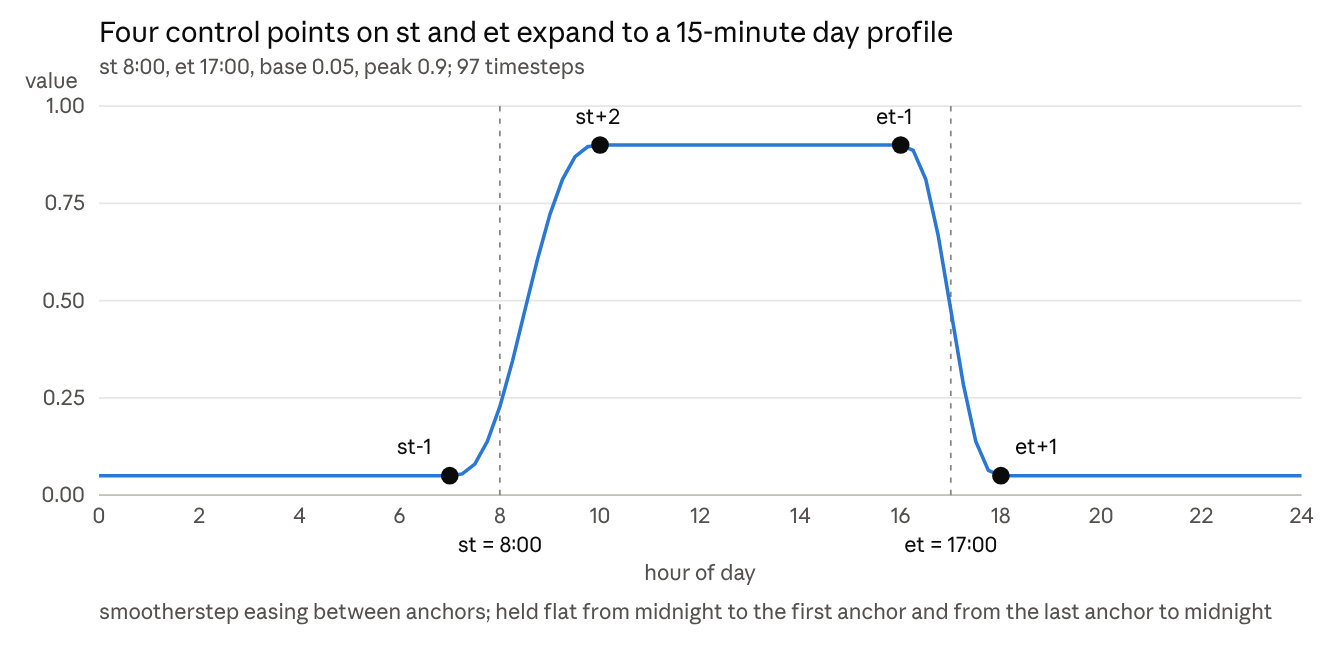
\includegraphics[width=0.9\textwidth]{figures/parametric_control_points.png}
    \caption[Expansion of a parametric schedule from control points]{Expansion of a parametric schedule from four control points placed relative to the operating start time (st) and end time (et). The sampled hours of operation set st and et; the control points are then interpolated to a 15-minute profile and held flat outside the first and last points.}
    \label{fig:parametric_control_points}
\end{figure}

\begin{figure}
    \centering 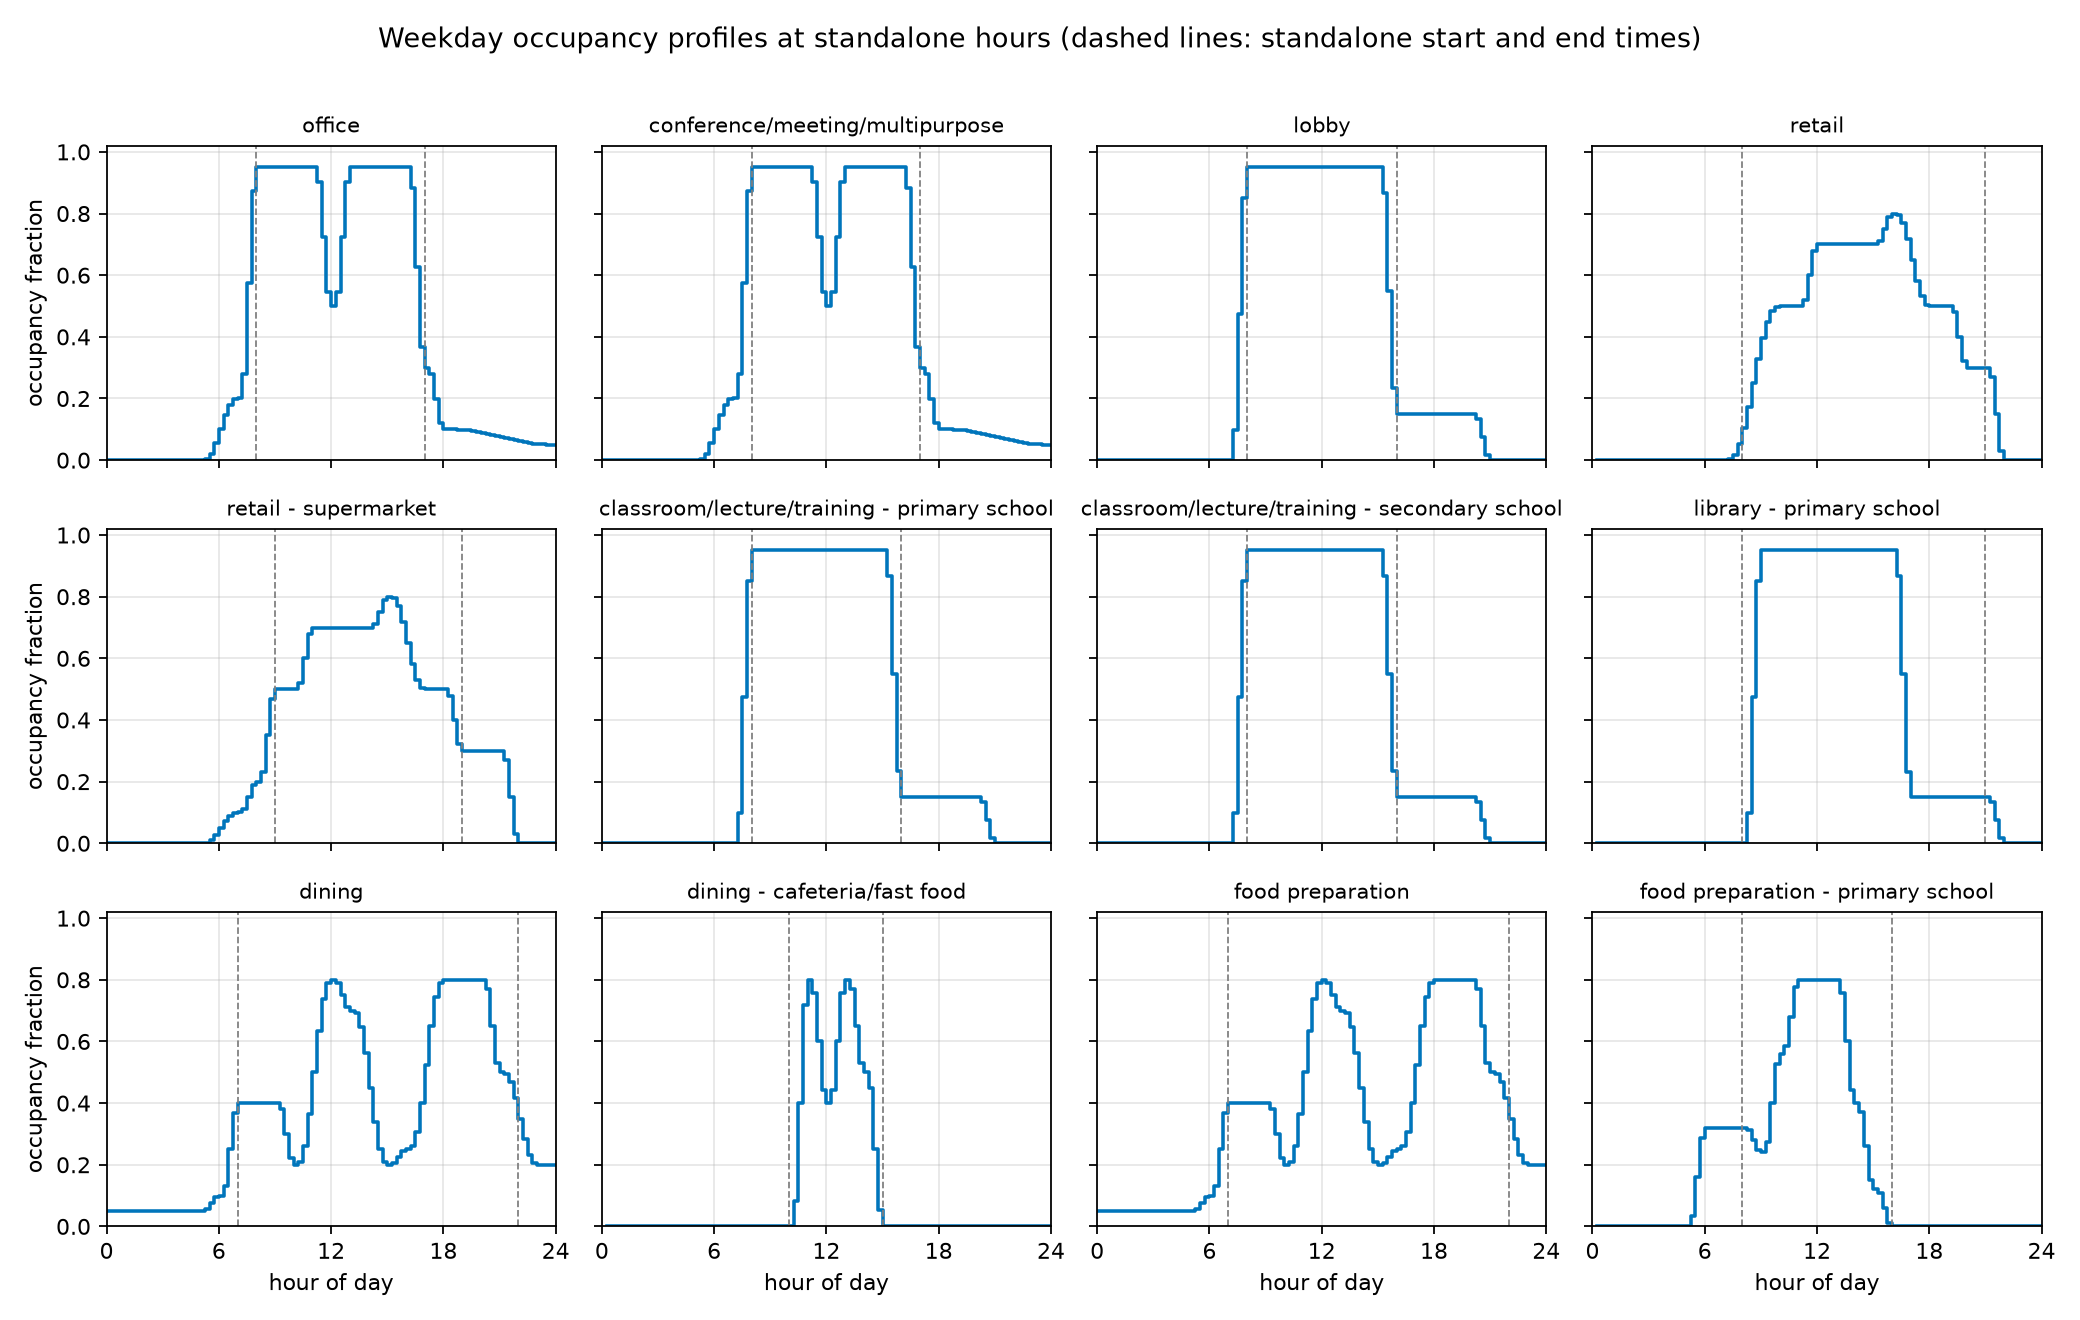
\includegraphics[width=1\textwidth]{figures/parametric_occupancy_1.png}
    \caption[Parametric weekday occupancy profiles, part 1]{Weekday occupancy profiles of office, retail, education, and food service space types, expanded at each schedule's standalone start and end times. In a model, the building's sampled hours of operation replace the standalone times.}
    \label{fig:parametric_occupancy_1}
\end{figure}

\begin{figure}
    \centering 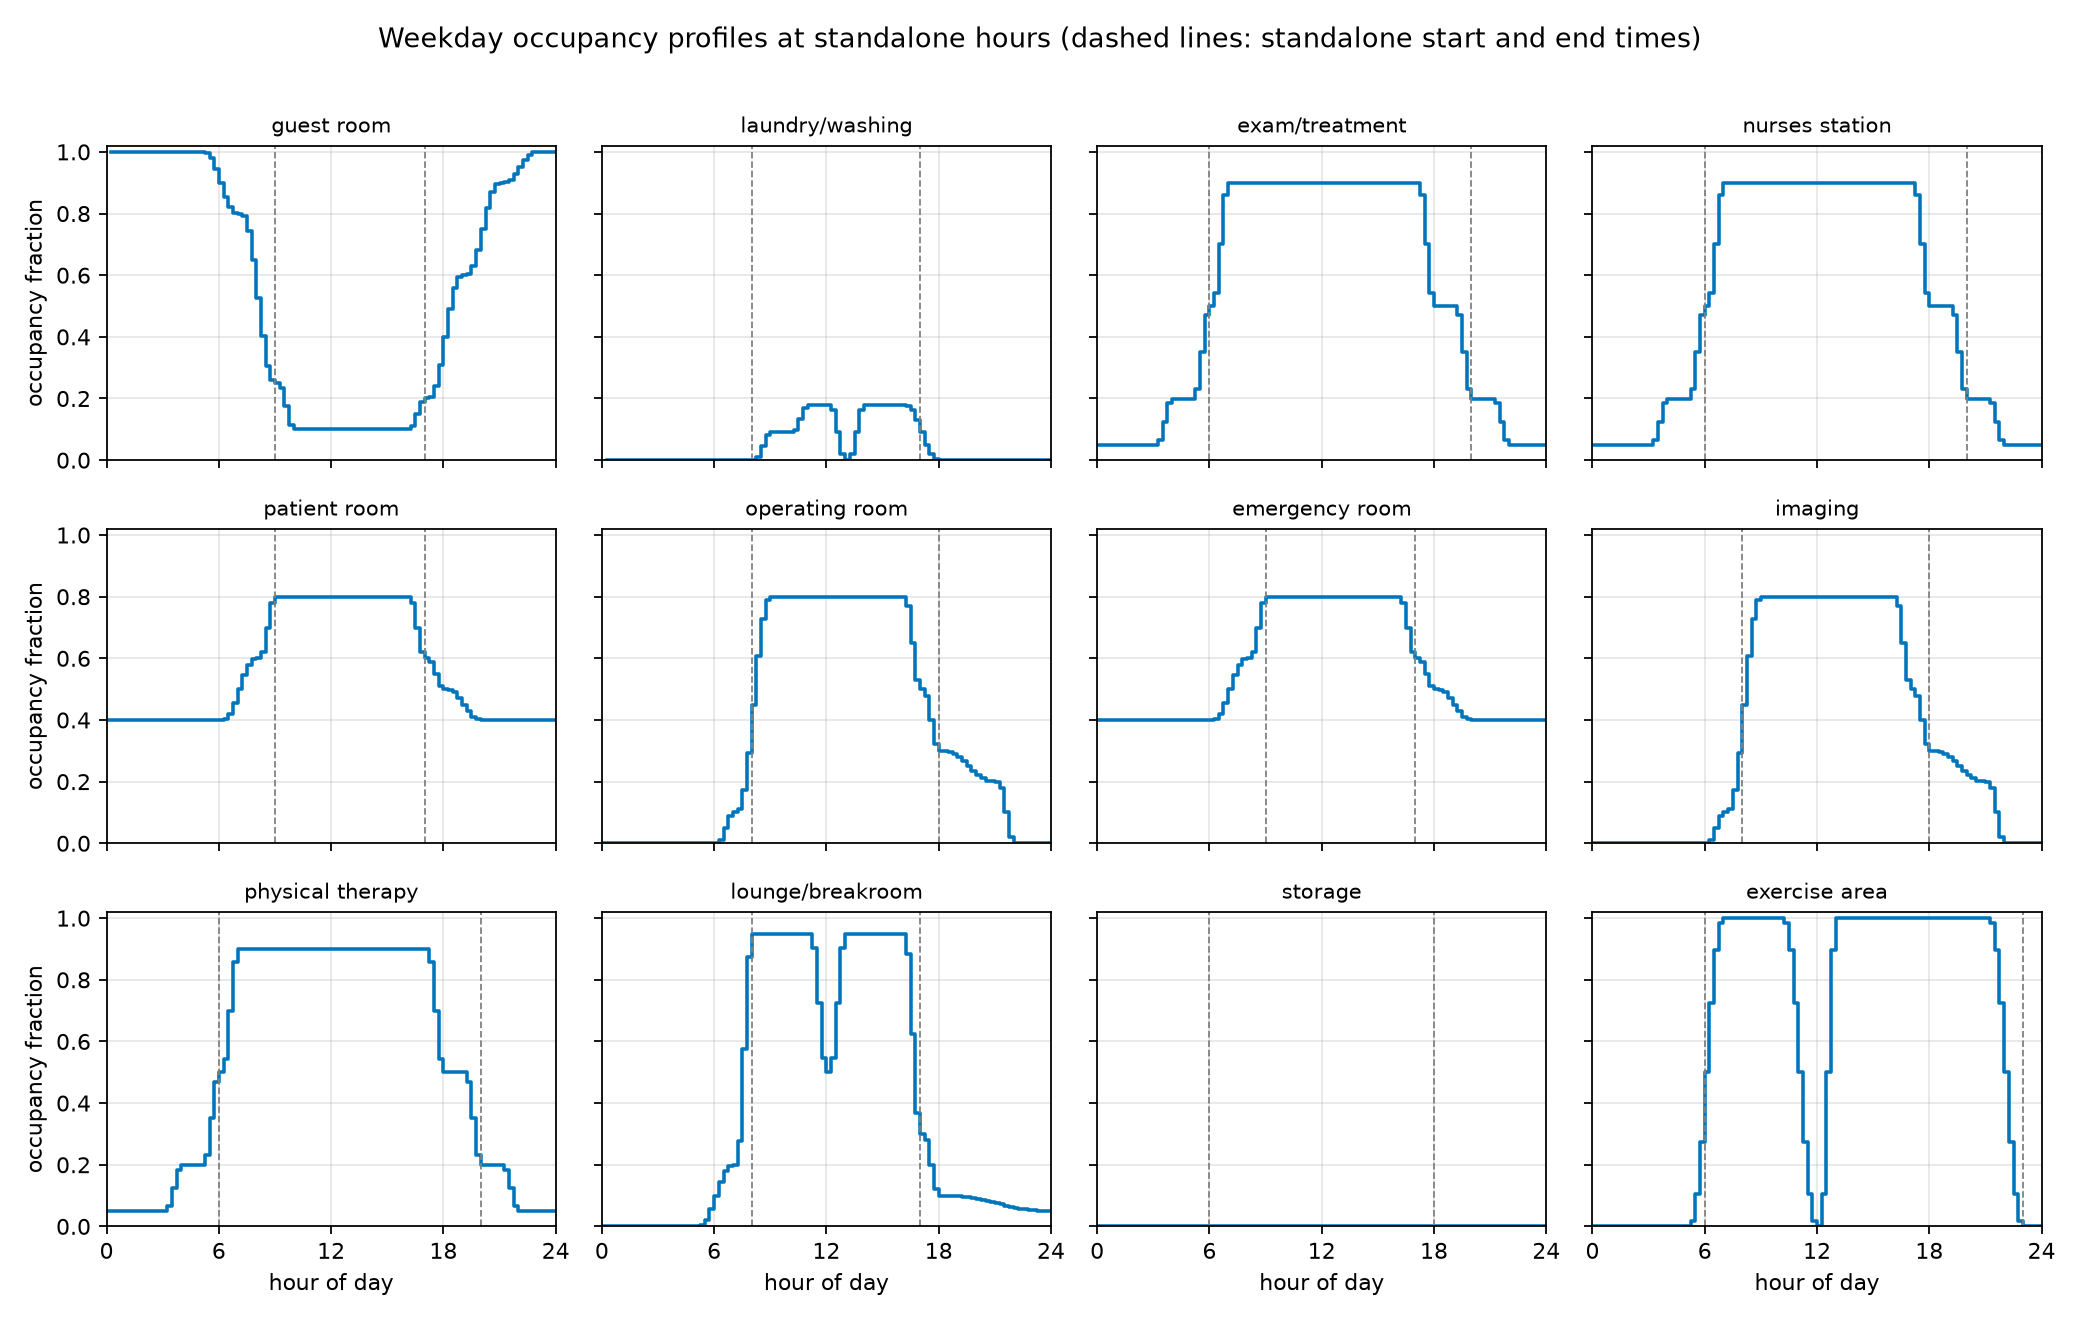
\includegraphics[width=1\textwidth]{figures/parametric_occupancy_2.png}
    \caption[Parametric weekday occupancy profiles, part 2]{Weekday occupancy profiles of lodging, healthcare, warehouse, and support space types, expanded at each schedule's standalone start and end times. Guest rooms and the hospital patient care space types keep their authored timing regardless of the building's hours of operation.}
    \label{fig:parametric_occupancy_2}
\end{figure}

\section{Geometry}
\subsection{General}
A building's geometry influences several aspects of its associated building energy model. It impacts the building envelope by dictating the orientation of windows, the surface-to-volume ratio, and the ratio of one surface type to another. Geometry also impacts how prevalent solar heat gain is for a given building through the building's orientation and shape. ComStock uses seven characteristics to define a building energy model's geometry: floor area, shape, aspect ratio, rotation, number of floors, floor height, and window-to-wall ratio (WWR). The majority of these characteristics are assigned to the models as part of the sampling process. Combined, they create a virtual building model geometry like the example shown in Figure~\ref{fig:geom_example}. All building models are variations of rectangular prisms with flat roofs and windows wrapping around the exterior. This simple geometry allows ComStock to easily scale properties and generate the number of individual building models needed for a national stock model. The following subsections describe each of the seven characteristics that define a building energy model's geometry in ComStock.

\begin{figure}[h!]
    \centering \includegraphics[width=0.7\textwidth]{figures/small_office_geometry.PNG}
    \caption[Example building geometry for a small office]{Example building geometry for a small office.}
    \label{fig:geom_example}
\end{figure}

\vspace{40mm} %blank space
\begin{center}
 (Intentionally blank)   
\end{center}


\pagebreak

\subsection{Area}
Building floor area is assigned to each model through the sampling process. Probability distributions were generated using CoStar \citep{costar} for most building types. HSIP \citep{hsip} was used for schools and hospitals, as neither are well represented in CoStar.

Figure~\ref{fig:area_dist} shows the breakdown of each building type in the national building stock by building size category (referred to as ``rentable area'').  Notice that the categories are presented as ranges.  At this time, ComStock uses the area in the middle of the range, with the exception of "\_1000" and "over\_1mil," which use 1000 square feet and 1 million square feet, respectively.  This method could be improved by adding variability to the building areas by selecting a variety of areas within the range.

\begin{figure}[H]
    \centering \includegraphics[width=1.0\textwidth]{figures/area_dist.png}
    \caption[Distribution of rentable area by building type]{Distribution of rentable area by building type. The x-axis represents rentable area (square feet), and the y-axis represents the fraction of the building stock.}
    \label{fig:area_dist}
\end{figure}

\pagebreak

\subsection{Building Shape}
Building shape is an intermediate characteristic assigned to the model during the sampling process. It is not a direct input to the model, as ComStock assumes a rectangular footprint for all buildings. Its function is as a dependency for aspect ratio (see next section \ref{subsec_aspect_ratio}). Probability distributions for building shape were generated from 2012 CBECS data, based on building type \citep{eia2012cbecs}. CBECS uses numbers to represent many of the answers to survey questions, and ComStock adopted these numbers to represent building shapes. 

Figure~\ref{fig:shape_dist} shows the breakdown of the national building stock by building shape and type. 

\begin{figure}[H]
    \centering \includegraphics[width=1.0\textwidth]{figures/shape.png}
    \caption[Distribution of building shape by building type.]{Distribution of building shape by building type. The x-axis represents the building shape, and the y-axis represents the fraction of the building stock.}
    \label{fig:shape_dist}
\end{figure}

\pagebreak

\subsection{Aspect Ratio} \label{subsec_aspect_ratio}
Aspect ratio is defined as the overall length in the east–west direction divided by the overall length in the north–south direction. It is assigned to the building models during the sampling process. Probability distributions based on building shape were generated from 2012 CBECS data \citep{eia2012cbecs}.

Figure~\ref{fig:aspect_ratio_dist} shows the breakdown of the national building stock by aspect ratio. The aspect ratios are integers from one to six, which represent a building's north-south:east-west ratio.

\begin{figure}[H]
    \centering \includegraphics[width=1.0\textwidth]{figures/aspect_ratio.png}
    \caption[Distribution of aspect ratio by building type]{Distribution of aspect ratio by building type. The x-axis represents the aspect ratio (an integer from 1--6), and the y-axis represents the fraction of the building stock.}
    \label{fig:aspect_ratio_dist}
\end{figure}

\pagebreak

\subsection{Rotation}
Rotation defines the orientation of the building relative to the cardinal directions. In ComStock, there are eight rotation options, ranging from 0 to 315 degrees at 45-degree intervals. Ninety and 270 degrees correspond to a north-south length and east-west width (Figure~\ref{fig:rotation}). Rotations are evenly distributed throughout the building stock due to a lack of available data for more detailed distributions. This will be improved if new data becomes available.

\begin{figure}[H]
    \centering \includegraphics[width=0.7\textwidth]{figures/rotation_example.png}
    \caption[Building rotation]{Illustration of building rotation. (a) Buildings with either 90 or 270 degree rotation have a north-south length. (b) Buildings with either 0 or 180 degree rotation have an east-west length.}
    \label{fig:rotation}
\end{figure}

\subsection{Floor Height}
Floor height is represented in the models as floor-to-floor height. Each building type definition carries a typical story height, and where the ground story differs a first-story height, taken from the DOE prototype buildings, which were established using expert opinion \citep{deru_2011}. These floor-to-floor heights are summarized in Table~\ref{tab:floor_height}. A space type may also carry its own story height within a building: the office portion of a warehouse is 14 feet tall rather than the 28 feet of the storage areas, and school gymnasia and auditoria are 26 feet tall.

\input{tables/floor_height}

\pagebreak

\subsection{Number of Floors}
ComStock assigns a number of floors to each model during the sampling process to create a distribution of building heights in the stock. This value represents the number of aboveground floors for a given model. No buildings in ComStock have belowground stories.

 For most of the building types, we generated probability distributions based on county and building type using CoStar \citep{costar}. We used HSIP \citep{hsip} for schools and hospitals, as neither are well-represented in CoStar.
 
 Figure~\ref{fig:nfloors_dist} shows the breakdown of the national building stock by number of floors and building type.

\begin{figure}[H]
    \centering \includegraphics[width=1.0\textwidth]{figures/nfloors.png}
    \caption[Distribution of number of aboveground  floors by building type]{Distribution of number of aboveground  floors by building type. The x-axis represents the number of floors, and the y-axis represents the fraction of the building stock.}
    \label{fig:nfloors_dist}
\end{figure}

\pagebreak

\subsection{Window-to-Wall Ratio (WWR)}
The ComStock window-to-wall ratio (WWR) assumptions were created as part of the EULP project. WWR is defined as the fraction of abovegrade wall area that is covered by fenestration. Previously, ComStock used the WWR from the DOE prototype building models. Although each building type had a different WWR, there was no variability within each building type, which is not representative of the building stock. To address this issue, we referenced the NFRC Commercial Fenestration Market Study conducted by Guidehouse \citep{guidehouse_nfrc_window_report}. The study characterized the national commercial window stock through data collection and analysis. Six primary data sources representing all regions of the United States were used in the study---a 2020 Guidehouse survey, NEEA CBSA, DOE Code Study, CAEUS, CBECS, and RECS (multifamily). A variety of window properties were collected, including WWR, number of panes, frame material, glazing type, low-emissivity coating, gas fill, and many others. In total, the database contained approximately 16,000 samples, each with an appropriate weighting factor based on the coverage, completeness, and fidelity of each data source. We incorporated the WWR results from this study into the ComStock model, and we may incorporate other fields in the future to further refine our window modeling methodology.

From the Guidehouse data, we developed a WWR distribution for each combination of building type, floor area, and vintage. We first analyzed the WWRs separately by building type, floor area, geographic location, and vintage to determine which filters were appropriate to use for the final distributions. Geographic location did not have a significant impact on WWR, so it was left out of the final distributions. As can be seen in Figures~\ref{fig:wwr_by_rentable_area} and~\ref{fig:wwr_by_building_vintage}, there is a noticeable change in the WWR of buildings built after 2014, indicating that new buildings are trending toward larger windows. Similarly, there is a distinct trend in the WWR as a function of floor area; larger buildings tend to have more windows. Whereas the previous methodology only varied WWR by building type, these new distributions introduce more WWR variability by considering vintage and floor area.

The WWR distributions for all buildings before and after incorporating the NFRC data are shown in Figure \ref{fig:wwr_before_after_all_buildings}. The distinct bins in the graph are a result of the way WWR is binned in the CBECS Show Card: 0\%--1\% WWR is binned to 0.0, 2\%--10\% to 0.06, 11\%--25\% to 0.18, 26\%--50\% to 0.38, 51\%--75\% to 0.63, and 76\%--100\% to 0.88. The final distributions do not change the stock total energy consumption significantly, but they do add realistic variability within building types. For example, previously, all large offices had the same WWR of 0.15, whereas using the new distributions, large office WWRs vary from 0.01 to 0.88.

    \begin{figure} [h]
    \centering \includegraphics[width=\textwidth]{figures/wwr_by_rentable_area.png}
    \caption[Window-to-wall ratio by rentable floor area]{Window-to-wall ratio by rentable floor area.}
    \label{fig:wwr_by_rentable_area}
    \end{figure} 

\pagebreak

    \begin{figure} [h]
    \centering \includegraphics[width=\textwidth]{figures/wwr_by_building_vintage.png}
    \caption[Window-to-wall ratio by building vintage]{Window-to-wall ratio by building vintage.}
    \label{fig:wwr_by_building_vintage}
    \end{figure} 

    \begin{figure}[h!]
    \centering \includegraphics[width=\textwidth]{figures/wwr_before_after_all_buildings.png}
    \caption[Window-to-wall ratio distribution]{Window-to-wall ratio distribution in all building types before and after incorporating NFRC data.}
    \label{fig:wwr_before_after_all_buildings}
    \end{figure} 

\pagebreak

\subsection{Space Programming and Thermal Zoning}
As described above, all ComStock building models are a rectangular prism with a prescribed aspect ratio, floor area, etc. Within each building, there are one or more space types, as described in Section \ref{sec:space_type_ratios}. Space types are represented within the rectangular geometry as ``slices'' through the building that correspond to the floor area fractions of each space type. This is shown in Figure \ref{fig:geometry_by_space_type_and_zone}(a). The space type flagged as the circulation space type in the building type definition is placed as a double-loaded corridor between the other slices rather than as a slice of its own. Space types that are exhausted (kitchens, laundries, restrooms) are sliced next to the space type that supplies their makeup air.

In very small buildings, slicing every space type in the definition would produce spaces that are unrealistically small and narrow for space types that make up only a small fraction of the building. Each space type category therefore carries a minimum floor area, below which the space type is not created and its floor area is absorbed by the space type flagged as the building type's default. Storage rooms, laundries, lobbies, corridors, restrooms, and mechanical rooms are dropped first; conference rooms, kitchens, dining rooms, and gymnasia next; and classrooms, patient and exam rooms, guest rooms, and retail sales floors are never dropped while any other space type is below its minimum. The consequence is that the smallest buildings in the stock are modeled with fewer, larger spaces than their building type definition lists, and the loads of a dropped space type are not represented in that building.

For larger buildings where the length and width are both greater than 37.5 feet, each space type is divided into core-and-perimeter thermal zones with a 15-foot depth (Figure \ref{fig:geometry_by_space_type_and_zone}(b)). Notice that the space types adjacent to the shorter ends of the building are each broken into six thermal zones, whereas the space types in the center of the building are each broken into three thermal zones. In multistory buildings, space types are often found on more than one floor, and in some cases, a floor will be a single space type. Buildings with three or more stories are modeled with a ground story, one mid story that carries a zone multiplier for the identical stories between the ground and top stories, and a top story, so that the number of thermal zones does not grow with the number of stories; the floors and ceilings between multiplied stories are adiabatic. The downside to this thermal zoning approach is that thermal zones---and, as a follow-on, the HVAC systems that serve them---may be unrealistically small or large for certain geometry and building type combinations.

\begin{figure}[hb!]
\centering \includegraphics[width=1\textwidth]{figures/geometry_by_space_type_and_zone.png}
\caption[Example building geometry]{Example building geometry colored by (a) space type and (b) zone.}
\label{fig:geometry_by_space_type_and_zone}
\end{figure} 
\section{Envelope}
\subsection{Walls} % Andrew
\paragraph{Wall Construction Type}
First, we selected the general types of wall construction methods to be represented in ComStock. We chose the four general wall types commonly used in commercial building energy codes because they cover the most common wall construction types and can be linked to nominal thermal characteristics. The definitions of these types from \cite{ashrae_901_2010} are as follows, with the corresponding ComStock enumerations shown in parentheses:

\begin{itemize}
\item \textbf{Mass wall} (Mass): A wall with a heat capacity exceeding (1) 7 Btu/ft\textsuperscript{2}·F or (2) 5 Btu/ft\textsuperscript{2}·F, provided that the wall has a material unit weight not greater than 120 lb/ft\textsuperscript{3}.
\item \textbf{Metal building wall} (Metal Building): A wall whose structure consists of metal spanning members supported by steel structural members (i.e., does not include spandrel glass or metal panels in curtain wall systems).
\item \textbf{Steel-framed wall} (SteelFramed): A wall with a cavity (insulated or otherwise) whose exterior surfaces are separated by steel  framing members (i.e., typical steel stud walls and curtain wall systems).
\item \textbf{Wood-framed and other walls} (WoodFramed): All other wall types, including wood stud walls.
\end{itemize}

To determine the prevalence of each wall construction type, we queried a database, \cite{lightbox_smartparcels_2021}, containing  building type, number of stories, location, and wall construction. The database did not use the same wall construction types selected for ComStock, so we created a mapping between the database entries and the wall construction types listed above, as shown in Table~\ref{tab:wall_construction_mapping}. Some construction types in the database were excluded from the mapping, either because the meaning was ambiguous or because they represented an insignificant fraction of the entries in the database. The excluded constructions represent only 5\% of the total samples, with 4.5\% labeled “OTHER” (which there was no clear way to map).

Upon reviewing the data, we identified two instances that were likely misclassifications. The first was buildings higher than five stories with the wall construction type``WoodFramed''. Historically, it was not possible to use WoodFramed construction for buildings over five stories, and even today, this practice is uncommon. Buildings with this combination were reassigned to ``Mass'' walls, based on the assumption that people were observing large wood internal structural members in old buildings and classifying them as WoodFramed. The second was buildings higher than two stories with ``MetalBuilding'' walls. Based on experience, this construction technique is commonly reserved for 1--2 story buildings only. Buildings with this combination were reassigned to ``SteelFramed,'' based on the assumption that this would be the most likely alternative classification if a person observed steel structural elements.

After mapping each entry in the database to one of the ComStock construction types, we analyzed the data to determine other building characteristics in the database were correlated with construction type. Older buildings were slightly more likely to use mass constructions, but the change over time was minor. Construction type varied significantly as a function of the number of stories. Shorter buildings were much more likely to be wood-framed, whereas taller buildings were more likely to be mass, and very tall buildings were likely to be steel-framed (steel studs or curtain wall). Based on a spot-checking of the database, we found the building type classification to be less reliable than other building characteristics. Although there was some correlation between building type and wall construction, there was also a correlation between building type and number of stories. Because of the joint correlation, we selected number of stories instead of building type. There was a clear correlation between climate zone and construction type---most notably, there was a much lower incidence of mass walls in cold climate zones. There was some correlation between construction type and building floor area. However, there was also a correlation between the number of stories and the building area. Because the construction type is physically limited by a building's height, it was more logical to use the number of stories as a driving characteristic for construction type. Following this analysis, we concluded that the number of stories and climate zone should be used as drivers of wall construction type. The probabilities for each combination of number of stories and climate zone were calculated  and then used as the input distribution for wall construction type in ComStock. This distribution is summarized in Table~\ref{tab:wall_constuction_types}.

\paragraph{Wall System Turnover Rate}
As described in Section~\ref{sec:system_turnover_and_eul}, we assume that some building systems, including exterior walls, are replaced over the lifespan of the building. Typically, for exterior walls, the structural elements of the wall are maintained, while the cladding, insulation, sheathing, etc. are be replaced. As noted in Section~\ref{sec:system_turnover_and_eul}, the EUL for exterior walls is assumed to be 200 years, which means that most buildings are modeled with the walls they were built with. Once the wall construction type probabilities and distributions of building types, sizes, and vintages are carried through the sampling process and simulations are created, the distribution of construction types and energy code levels can be reviewed. As shown in Figure~\ref{fig:weighted_floor_area_by_energy_code_and_wall_type}, because the majority of the building stock is older, and wall systems are replaced at a low rate, most of the building floor area is assumed to have walls that follow the oldest energy codes.

\begin{figure}[ht!] \centering
    \includegraphics[
        width=\textwidth]{figures/weighted_floor_area_by_energy_code_and_wall_type.png}
    \caption[Weighted floor area by energy code followed during last wall replacement and wall type]{Weighted floor area by energy code followed during last wall replacement and wall type.}
    \label{fig:weighted_floor_area_by_energy_code_and_wall_type}
\end{figure}
\vspace{2mm}
\paragraph{Wall Thermal Performance}
We did not find any data sources that contained the thermal performance (U-Value/R-Value) of walls in the commercial building stock. This is likely because surveys would need to either find building plans, which can be difficult or impossible for older buildings, or disassemble part of the structure to look inside the walls, which building owners are unlikely to allow. To account for the lack of data, we estimated wall thermal performance based on an estimate of the energy code followed when the wall was last replaced. Section~\ref{sec:energy_code} describes how the energy code was determined. The thermal performance of walls for each energy code varies based on climate zone and construction type, as shown in Table~\ref{tab:wall_r_values} and Table~\ref{tab:wall_r_values_deer}. Note that although these thermal performance values do include the thermal bridging inherent in the clear field wall, they do not include thermal bridging at intermediate floors, parapets, and glazing transitions. These additional thermal bridges are expected to lower the overall thermal performance of the wall assembly.

As previously described, most of the building stock's walls are assumed to be older. Therefore, the thermal performance assumptions for older vintages have a much higher impact on the overall heating and cooling demand than those for newer vintages. The ComStock DOE Ref Pre-1980 assumptions, taken from \cite{doe_reference_buildings}, are originally from a study of only offices \citep{old_vintage_office_study}. Unfortunately, this study no longer appears to be available. Following the methodology in \cite{doe_reference_buildings}, these values are used for all wall construction types and all building types. Figure~\ref{fig:weighted_floor_area_by_building_type_and_wall_type} shows the final prevalence of each wall construction type by building type. Most notable is the low prevalence of metal building walls across the stock, even in warehouses. This might be surprising, but it is supported by the available data. Table \ref{tab:wall_r_value_averages} shows the average wall thermal performance by ASHRAE Standard 169--2006 climate zone.

\begin{figure}[ht!] \centering
    \includegraphics[
        width=\textwidth]{figures/weighted_floor_area_by_building_type_and_wall_type.png}
    \caption[Weighted floor area by wall type and building type]{Weighted floor area by wall type and building type.}
    \label{fig:weighted_floor_area_by_building_type_and_wall_type}
\end{figure}

\vspace{2mm}

\subsection{Windows} % Andrew
\paragraph{Window Construction Type}
Data from the NFRC Commercial Fenestration Market Study was used to develop the modeling approach for windows in ComStock. This study, conducted by Guidehouse in collaboration with NFRC, characterized the national commercial window stock through data collection and analysis. Six primary data sources representing all regions of the United States were used in the study---a 2020 Guidehouse survey, NEEA CBSA, DOE Code Study, CAEUS, CBECS, and RECS. A variety of window properties were collected, including the window-to-wall ratio, number of panes, frame material, glazing type, low-E coating, gas fill, solar heat gain coefficient (SHGC), U-factor, and many others. In total, the database contained approximately 16,000 samples, each with an appropriate weighting factor based on the coverage, completeness, and fidelity of each data source. The WWR data was already incorporated into the ComStock baseline during the EULP project. Some of the other key window properties such as thermal performance were then used to create the new baseline window constructions and distributions discussed later in this section. A summary of the data sources and their associated information is shown in Table ~\ref{tab:window_data_sources}.

Four window properties---number of panes, glazing type, frame material, and low-E coating---were used to create the baseline window configurations. These four parameters were selected based on which characteristics have the most impact on window performance, which have the most data available from the various data sources, and which inputs we trust from the average building owner or survey recipient. The options for each property are shown in Figure \ref{fig:window_configurations}.

\begin{figure}[ht!] \centering
    \includegraphics[
        trim={0cm 0cm 0cm 0cm}, clip, % L B R T
        width=0.5\textwidth]{figures/window_configurations.png}
    \caption{Window characteristics for number of panes, glazing type, frame material, and low-E coating.}
    \label{fig:window_configurations}
\end{figure}
\vspace{5mm}

Modeling every combination of these four properties would result in 36 different window configurations, which would add significant complexity to the sampling process. Instead, we selected 12 combinations to be modeled, based on which combinations are most common and most realistic. There are four single-pane, six double-pane, and two triple-pane configurations. The unrealistic/uncommon combinations that were eliminated include:
\begin{itemize}
\item Single pane with thermally broken aluminum frame
\item Single pane with low-E coating
\item Double pane with wood frame
\item Triple pane with no low-E coating
\item Triple pane without thermally broken aluminum frame
\item Thermally broken double or triple pane without low-E coating.
\end{itemize}
The 12 remaining window configurations are shown in Table \ref{tab:window_configurations}.

\input{tables/window_configurations}

We created a sampling distribution for the new window constructions for the entire country using the initial data set. Overall, single-pane windows make up approximately 54\% of the stock, double-pane windows make up 46\%, and triple-pane windows make up <1\%. Initially, we created distributions based on census division to incorporate geographic location into the sampling. Upon further analysis, we found that it was also necessary to incorporate the energy codes into distributions to prevent scenarios where a single-pane window was sampled for a certain location, but, according to the energy code for that location, a double-pane window was required. For this reason, we modified the sampling distribution to include two dependencies---climate\_zone and  energy\_code\_followed\_during\_last\_window\_replacement.

To generate these sampling distributions, we used the maximum U-values specified for each climate zone in each version of ASHRAE 90.1, using climate zones defined by ASHRAE 169--2006. For each combination of climate zone and energy code, the 12 window configurations were evaluated to determine which were both realistic and met code (i.e., had a U-value lower than the code maximum U-value). For the older energy codes, we made several assumptions about technology adoption to determine which window configurations were realistic:
\begin{itemize}
    \item Low-E coating---not adopted until DOE Ref 1980--2004
    \item Thermally broken aluminum frame---not adopted until 90.1-2004
    \item Triple pane---not adopted until 90.1-2004.
\end{itemize}

Each combination of climate zone and energy code included 2--12 window configurations that met the criteria. After limiting the distributions to these configurations, we renormalized the percentages from the national distribution to 100\%. This kept the percentages from the national distribution while also incorporating intelligent assumptions based on climate zone and energy code. Table ~\ref{tab:window_distribution_4A} provides an example of the window configurations that were sampled for each code year in climate zone 4A.

\input{tables/window_distribution_4A}

As can be seen in Table \ref{tab:window_distribution_4A}, for DOE Ref Pre-1980, the only windows that met code and are realistic are single-pane or double-pane windows with no low-E coating. For DOE Ref 1980--2004, the maximum U-value dropped significantly, such that single-pane aluminum windows no longer met code. However, double-pane low-E windows became available on the market at that time. For 90.1-2004 through 90.1-2010, code required a U-value equivalent to double-pane low-E or better, and in 90.1-2013, the code improved again, meaning that double-pane low-E with a thermal break or better was required. This type of logic was applied to all combinations of climate zone and energy code. Then, we converted the data into the distributions used in sampling.

A small adjustment was made to the final distributions because some states and localities do not follow or enforce energy codes strictly. Following the code exactly would likely overestimate window performance. Therefore, in scenarios where single-pane windows were technically below code, we assumed that 5\% of all windows in the stock would still have the worst-performing single-pane windows installed. The distributions were adjusted accordingly by subtracting 5\% total from the double-pane configurations and adding to the single-pane aluminum configurations. After making this manual adjustment, the new distributions had the same overall breakdown as the national distribution generated from the Guidehouse data---54\% single-pane and 46\% double-pane .

\paragraph{Window Thermal Performance}
Once the 12 new window constructions were determined, a team from Lawrence Berkeley National Laboratory's (LBNL’s) Windows and Daylighting Group used the WINDOW program to assign thermal performance properties to each construction. SimpleGlazing objects in EnergyPlus were chosen to represent windows to reduce complexity. This choice also simplifies the process of applying upgrades, because all fenestration objects in the baseline models use the same object type. The inputs for the SimpleGlazing object are U-factor, solar heat gain coefficient (SHGC), and visible light transmittance (VLT). For each window configuration, LBNL assigned a frame ID and window ID from the WINDOW database. They also filled in the respective U-factors, SHGCs, and VLTs, which are shown in Table \ref{tab:window_thermal_performance}.

The U-factors originally ranged from U-1.18 Btu/h·ft\textsuperscript{2}·F for the worst-performing single-pane window to U-0.30 Btu/h·ft\textsuperscript{2}·F for the best-performing triple-pane window. As mentioned earlier in this section, the maximum U-Factor that EnergyPlus can model with a simple glazing object is U-1.02 Btu/h·ft\textsuperscript{2}·F, which is governed by the limitations of a 2D heat transfer model when interior and exterior air films are included. Therefore, we adjusted the U-factor for the first two single-pane windows to be U-1.02 Btu/h·ft\textsuperscript{2}·F rather than U-1.18 Btu/h·ft\textsuperscript{2}·F. This allowed these windows to be modeled in ComStock. This results in a slight overestimate of the thermal performance of single-pane windows.


\subsection{Roof} % Andrew
\paragraph{Roof Construction Type}
First, we reviewed the general types of roof construction methods that could be represented. The three general roof types commonly used in commercial building energy codes were chosen because they cover the most common roof construction types and can be linked to nominal thermal characteristics. The definitions of these types from \cite{ashrae_901_2010} are as follows:

\begin{itemize}
\item \textbf{Roof with insulation entirely above deck (IEAD)}: A roof that has all insulation installed above (outside of) the roof structure and that is continuous (i.e., uninterrupted by framing members).
\item \textbf{Metal building roof}: A roof that is constructed with a metal, structural weathering surface; has no ventilated cavity; and has the insulation entirely below deck (i.e., does not include composite concrete and metal deck construction or a roof framing system that is separated from the superstructure by a wood substrate). In addition, the roof structure consists of one or
more of the following configurations: (a) metal roofing in direct contact with the steel framing members, (b) metal roofing separated from the steel framing members by insulation, or (c) insulated metal roofing panels installed as described in a or b.
\item \textbf{Attic and other roof}: All other roofs, including roofs with insulation entirely below (inside of) the roof structure (e.g., attics, cathedral ceilings, and single-rafter ceilings); roofs with insulation both above and below the roof structure; and roofs without insulation (excluding metal building roofs).
\end{itemize}

The analysis of roof properties in \cite{eia2012cbecs}, shown in Figure~\ref{fig:cbecs_floor_area_by_roof_tilt_and_attic_presence}, indicates that about 90\% of the commercial floor space covered by ComStock has flat or shallow pitch roofs, and that the large majority of the buildings with flat or shallow pitch roofs do not have attic space. Given these factors and the complexity associated with modeling the geometry of pitched roofs, we decided to model the entire stock as having flat roofs.

\begin{figure}[h] \centering
    \includegraphics[
        trim={0cm 1.5cm 0cm 0cm}, clip, % L B R T
        width=\textwidth]{figures/cbecs_floor_area_by_roof_tilt_and_attic_presence.png}
    \caption{Weighted floor area by roof tilt and attic presence.}
    \label{fig:cbecs_floor_area_by_roof_tilt_and_attic_presence}
\end{figure}

\vspace{5mm}
No data sources for roof construction type were found. The roof construction type is named in each building type definition (Section~\ref{sec:building_spec}) by template family. As shown in Table~\ref{tab:roof_construction_types}, most buildings are assumed to use IEAD roofs, which is consistent with the assumption of flat roofs; restaurants use attic-and-other roofs. Under the DEER templates assigned to California buildings, the definitions carry the roof and interior construction types of the DEER prototype buildings \citep{cpuc_deer}.

\paragraph{Roof System Turnover Rate}
As described in Section \ref{sec:system_turnover_and_eul}, some building systems, including roofs, are assumed to be replaced over the lifespan of the building. Typically, for roofs, the structural elements are maintained, while the roof membrane and insulation are replaced. As noted in Section \ref{sec:system_turnover_and_eul}, the EUL for roofs was assumed to be 200 years, which means that most buildings are modeled with the roof insulation they were built with. Once the roof type probabilities and distribution of building types, sizes, and vintages are carried through the sampling process and simulations are created, the distribution of energy code levels can be reviewed. As shown in Figure~\ref{fig:weighted_floor_area_by_energy_code_roofs}, because the majority of the building stock is older, and roof systems are replaced at a low rate, most of the building floor area is assumed to have roofs that follow the oldest energy codes.

\begin{figure}[h] \centering
    \includegraphics[
        width=\textwidth]{figures/weighted_floor_area_by_energy_code_roofs.png}
    \caption{Weighted floor area by energy code followed during last roof replacement.}
    \label{fig:weighted_floor_area_by_energy_code_roofs}
\end{figure}
\vspace{5mm}
\paragraph{Roof Thermal Performance}
We did not find any data sources that contained the thermal performance (U-Value/R-Value) of roofs in the commercial building stock. This is likely because surveys would need to either find building plans, which can be difficult or impossible for older buildings, or disassemble part of the structure to look inside the roofs, which building owners are unlikely to allow. To account for the lack of data, we estimated roof thermal performance based on an estimate of the energy code followed when the roof was last replaced. Section~\ref{sec:energy_code} describes how the energy code was determined. The thermal performance of roofs for each energy code varies based on climate zone and construction type, as shown in Tables~\ref{tab:roof_r_values} and \ref{tab:roof_r_values_deer}. While these thermal performance values do include the thermal bridging inherent in the clear field roof, they do not include thermal bridging at parapets, skylight curbs, or roof penetrations for HVAC systems. These additional thermal bridges are expected to lower the overall thermal performance of the roof assembly.

As previously described, most of the building stock's roofs are assumed to be older. Therefore, the thermal performance assumptions for older vintages have a much higher impact on the overall heating and cooling demand than the assumptions for newer vintages. The ComStock DOE Ref Pre-1980 assumptions, taken from \cite{doe_reference_buildings}, are originally from a study of only offices \citep{old_vintage_office_study}. Unfortunately, this study no longer appears to be available. Following the methodology in \cite{doe_reference_buildings}, these values are used for all roof construction types and all building types.


\subsection{Floor}
In ComStock, all buildings are assumed to be built using slab-on-grade construction and to have no cantilevered thermal zones. Thus, the only heat transfer into the building through floors is assumed to happen through the floor in contact with the ground. All floors between stories are internal surfaces, and any heat transfer through these surfaces occurs between zones within the building, not between the building and the outside environment.

\paragraph{Floor Thermal Performance}
We did not find any data sources that contained the thermal performance of floors in the commercial building stock. This is likely because surveys would need to either find building plans, which can be difficult or impossible for older buildings, or excavate under a slab edge, which is impractical. To account for the lack of data, we estimated floor thermal performance based on an estimate of the energy code followed when building was first constructed. Section~\ref{sec:energy_code} describes how the energy code was determined. The thermal performance of floors for each energy code varies based on climate zone, as shown in Table~\ref{tab:floor_f_factors}. It is notable that only buildings built to the newest energy codes in the coldest climates assume any sort of slab insulation.

\subsection{Thermal Bridging} % Matthew Dahlhausen
Thermal bridging includes the impact of uninsulated structural elements that undermine the overall thermal resistance of an opaque assembly. These include linear thermal bridges, such as along corners, roof parapets, and fenestration, and point thermal bridges, such as protruding steel beams. These are formalized by psi factors multiplied by the length of a thermal bridge, and chi factors multiplied by the number of a thermal bridge. ASHRAE publishes psi and chi factors for common major thermal bridges, and thermal bridging requirements were recently added to the envelope section of ASHRAE 90.1-2022 \citep{ashrae_901_2022}. See Appendix section A10.2 of ASHRAE 90.1-2022 for details on calculating thermal bridges.

Thermal bridging in ComStock is implemented with the Thermal Bridging and Derating (TBD) ruby gem \citep{tbd_gem}. The gem detects the presence of common major thermal bridges in the model (corners, parapets, etc.), and derates the adjacent opaque surface construction (walls and roofs) to account for the thermal bridging. TBD gem version 3.4.1 includes default ASHRAE 90.1-2022 psi and chi factors for different kinds of thermal bridges. These vary by wall construction type (steel frame, mass, wood) and whether thermal bridges are considered mitigated or unmitigated. By default, ComStock assumed the unmitigated 90.1-2022 psi and chi factors by wall construction type. Specific values are listed in the TBD gem \citep{tbd_gem}.

\subsection{Infiltration and Natural Ventilation} % Matthew Dahlhausen

\subsubsection{Infiltration}
Infiltration in ComStock uses the same model as EnergyPlus \citep{energy_plus}, detailed in equation \ref{energyplus_infiltration_eqn}.

\begin{align}
\label{energyplus_infiltration_eqn}
Infiltration = I_{design} * F_{schedule} * [A + B * |(T_{zone} - T_{odb})| + C * WindSpeed + D * WindSpeed^2]
\end{align}

where:\\
\begin{itemize}
\item \textbf{I\textsubscript{design}} is the design infiltration flow rate, in m\textsuperscript{3} per s per m\textsuperscript{2} exterior surface area\\
\item \textbf{F\textsubscript{schedule}} is a fractional schedule, usually tied to HVAC system operation\\
\item \textbf{A} is the coefficient for constant infiltration\\
\item \textbf{B} is the coefficient for temperature difference driven infiltration\\
\item \textbf{T\textsubscript{zone}} is the zone air temperature, in degrees Celsius\\
\item \textbf{T\textsubscript{odb}}  is the outdoor dry bulb temperature, in degrees Celsius\\
\item \textbf{C} and \textbf{D} are linear and quadratic coefficients for wind driven infiltration\\
\item \textbf{WindSpeed} is the local windspeed, in m per s.\\
\end{itemize}

The selection of the design infiltration rate is somewhat arbitrary, as it depends on the assumed natural pressure at typical conditions. The coefficients need to be paired with an assumed natural pressure.

\subsubsection{Infiltration Rates}
Infiltration rates are calculated from measured airtightness data from \citep{nist_infiltration_data}. There are significant differences in building airtightness due to differences in wall construction, shown in Figure 6 of the NIST reference. Airtightness does not vary significantly by building type or vintage. Airtightness does depend on size, but this is inherently captured by larger buildings having smaller surface area to volume ratios. Air barriers greatly reduce leakiness, but they are rare in existing buildings, and only recently have been required in some jurisdictions. Airtightness of buildings in ComStock follow lognormal distributions with airtightness means by wall construction type matched to those in \citep{nist_infiltration_data}, shown in Figure \ref{fig:airtightness_by_wall_construction_type}.
Airtightness values are measured at 75 Pa and are 6-sided, meaning the infiltration is normalized by total building exterior surface area including wall, roof, and ground surfaces.

The design infiltration rate is calculated from the airtightness value assuming a 4 Pa design pressure, shown in \ref{airtightness_to_design_infiltration}
\begin{align}
\label{airtightness_to_design_infiltration}
I_{\text{design}} = \text{airtightness} \cdot \left(\frac{1\ \text{hr}}{3600\ \text{s}}\right) \cdot \left(\frac{5\ \text{sided area}}{6\ \text{sided area}}\right) \cdot \left(\frac{4.0\ \text{Pa}}{75.0\ \text{Pa}}\right)^{0.65}
\end{align}
where:\\
\begin{itemize}
\item \textbf{airtightness} is the measured airtightness at 75 Pa in m\textsuperscript{3} per hr per m\textsuperscript{2} 6-sided exterior surface area\\
\item \textbf{I\textsubscript{design}} is the design infiltration rate at 4 Pa in m\textsuperscript{3} per s per m\textsuperscript{2} 5-sided exterior surface area\\
\end{itemize}

\begin{figure}
    \centering \includegraphics[width=0.9\textwidth]{figures/airtightness_by_wall_construction_type.png}
    \caption[Airtightness by Wall Construction Type]{6-sided airtightness distributions by wall construction type. Distributions are lognormal, with means matched to means by wall construction type in \citep{nist_infiltration_data}.}
    \label{fig:airtightness_by_wall_construction_type}
\end{figure}

\subsubsection{Infiltration Coefficients}
\label{sec:infiltration_coefficients}
NIST derived coefficients by building CONTAM models of all of the DOE prototype buildings, as explained in \citep{nist_infiltration_correlations}. The coefficients assume a 4 Pa design pressure. The coefficients include A, B, and D terms, with C being 0. Coefficients are by building type, with separate coefficients for whether the HVAC system is on or off; this is one of the few places where a load in the model is keyed on the building type rather than on its space types. The NIST report includes separate coefficients for buildings with air barriers, but ComStock does not assume buildings have air barriers. The HVAC-off coefficients apply through an infiltration schedule that is the inverse of the HVAC operation schedule, so that a seasonal HVAC rule produces a matching seasonal infiltration rule.

NIST did not model all DOE prototype buildings, and does not include HVAC system off coefficients for some buildings if the prototype was modeled as always on. ComStock building types not available in the NIST data use coefficients for either the Office or Retail building types. If off coefficients are not available, the building uses the on coefficients instead.
\subsubsection{Natural Ventilation}

Natural ventilation is not modeled in ComStock because it is not common in the building stock.

\section{Lighting}
\subsection{Interior Lighting}
Interior lighting follows a technology baseline approach, meaning that energy consumed by lighting is set by an assumed distribution of a particular lighting technology (e.g., T8 or linear LEDs), rather than following a lighting power density (LPD) allowance defined in a specific energy code version. The technology baseline approach recognizes that buildings typically do not use their full lighting power allowance. It also explicitly labels lighting technology and subsystems in the energy model for granular energy efficiency measure analysis.

Two components specify interior lighting: the lighting power density and the interior lighting schedule.  The lighting power density is determined by the distribution of lighting technologies in the stock, the lighting technology properties, and the space type properties. The lighting schedule is determined by a default lighting schedule by space type, occupancy hour adjustments, and magnitude variability.

\subsubsection{Determining Lighting Power}
The technology baseline approach follows a similar process to how the ASHRAE 90.1 lighting subcommittee determines the LPD allowance for a given space type in ASHRAE 90.1. In the lighting subcommittee model (LSM), there are four kinds of lighting systems that together contribute to a target horizontal illuminance:

LPD = General Lighting + Task Lighting + Supplemental Lighting + Wall Wash Lighting \\

\begin{align}
\label{lsm_lpd_eqn}
LPD = \frac{\% LS_{1} \cdot fc}{RSDD \cdot TF_{1}} + \frac{\% LS_{2} \cdot fc}{RSDD \cdot TF_{2}} + \frac{\% LS_{3} \cdot fc}{RSDD \cdot TF_{3}} + \frac{\% LS_{4} \cdot fc}{RSDD \cdot TF_{4}}
\end{align}
where:\\
\begin{itemize}
\item \textbf{\%LS\textsubscript{i}} is the percent of the target horizontal illuminance value met by a specific lighting system\\
\item \textbf{fc} is the target horizontal illuminance value in lumens per ft\textsuperscript{2}\\
\item \textbf{RSDD} is room surface dirt depreciation, an estimate of how much surface dirt reduces light from reaching the horizontal plane\\
\item \textbf{TF\textsubscript{i}} is the total lighting factor, where TF = source luminous efficacy * coefficient of utilization * lighting loss factor (LFF)\\
\item \textbf{Source luminous efficacy} is the lighting technology efficacy in lumens per watt\\
\item \textbf{Coefficient of utilization} is a term that captures how much lighting from the luminaire reaches the horizontal plane\\
\item \textbf{LLF} is the lighting loss factor, where LLF  = luminaire dirt depreciation (LDD) * lamp lumen depreciation (LLD)\\
\end{itemize}

Values for all these terms are specified in the LSM.  The LSM is exact, using a specific lighting product, room geometry, distribution of lighting systems, and other properties to determine the lighting power density allowance for a given space type. ComStock differs from the LSM in several important ways.

First, ComStock generalizes lighting technology (e.g., T8 linear fluorescent luminaires for general lighting) rather than modeling a specific lighting product.  Source efficacy, lighting loss properties, and radiant fractions are tied to lighting technology. Source efficacy values come from \cite{doe2015lmc} for older lighting technologies and \cite{doe2019ssl} for LEDs.  Radiant heat gain fractions come from \cite{ashrae_rp1282} for older lighting technologies and \cite{ashrae_rp1681} for LEDs.

Second, lighting technologies are broken out into lighting generations depending on the most common space lighting technology in that generation, as general lighting accounts for most ($\sim$80\%--90\%) of total lighting. High bay is treated as general lighting, and the lighting measure uses the general high bay technology for rooms with height $\ge$20 ft. Lighting generations 4--8 are all LED, with improving efficacy over time. Lighting generations and their technologies are detailed in Table \ref{tab:int_light_gens}, and lighting technology properties are detailed in Table~\ref{tab:int_light_techs_all}.

Third, the coefficient of utilization depends on both the luminaire properties and the room geometry, which complicates the calculation in the LSM. The ComStock model associates the coefficient of utilization entirely with room propertiesthat are independent of lighting technology.  ComStock further assumes that rooms of the same space type have similar enough properties that they can use the same coefficient of utilization. To retain some of the variation from the luminaire properties, each kind of lighting system has a different coefficient of utilization for each space type.

Table~\ref{tab:int_light_space_types} in Appendix~\ref{appendix:a} details the target horizontal illuminance value, the fraction of the target illuminance met by the kind of lighting system, and the lighting system coefficient of utilization for each lighting space type. Lighting space types are the space-by-space categories defined in ASHRAE 90.1, and every space type names its lighting space type directly, so no mapping from a building type's space types is involved. A space type's average ceiling height, computed from the model geometry, selects between standard and high bay fixtures for the general lighting system.

Fourth, the LSM assumes a high fraction of non-general lighting systems for certain space types. For example, half of the illuminance in retail sales spaces is from supplemental and wall wash lighting systems. In older lighting generations, there is a significant difference in source efficacy between general and non-general lighting systems. In lighting generation 2, general lighting assumes T8 linear fluorescent lamps at 94 lumens per watt, and supplemental and wall wash lighting assume halogens at 15 lumens per watt.  For retail spaces using the LSM values, that means half the lighting comes from lighting technologies roughly 6 times less efficient than the general lighting technology.  Although this may be appropriate for setting a code lighting allowance, most retail spaces meet a much greater percentage of their illuminance from more efficient general lighting technologies.  ComStock adjusts the lighting system fractions for commonly used space types so that around 80\%--90\% of lighting comes from the general lighting system. These changes are reflected in Table~\ref{tab:int_light_space_types} in Appendix \ref{appendix:a}.

Lastly, the LSM offers a generous allowance for lighting power density to account for the lighting loss factor over time. Including lighting losses and depreciation can result in a lighting power density ~40\% higher than when these terms are ignored. This resulted in unreasonably high installed lighting power densities; thus, ComStock assumes that most existing lighting systems were not designed to account for depreciation over time, and therefore excludes lighting loss and depreciation terms from the lighting power calculation.

With these changes, the LPD calculation simplifies to:
\begin{align}
\label{comstock_lpd_eqn}
LPD = \frac{\% LS_{1} \cdot fc}{\text{efficacy} \cdot CU_{1}} + \frac{\% LS_{2} \cdot fc}{\text{efficacy} \cdot CU_{2}} + \frac{\% LS_{3} \cdot fc}{\text{efficacy} \cdot CU_{3}} + \frac{\% LS_{4} \cdot fc}{\text{efficacy} \cdot CU_{4}}
\end{align}

where:\\
\begin{itemize}
\item \textbf{\%LS\textsubscript{i}} is the percent of the target horizontal illuminance value met by a specific lighting system\\
\item \textbf{fc} is the target horizontal illuminance value in lumens per ft\textsuperscript{2}\\
\item \textbf{Efficacy} is the source luminous efficacy of the lighting technology in lumens per watt\\
\item \textbf{CU} is the coefficient of utilization, a term that captures how much lighting from the luminaire reaches the horizontal plane.\\
\end{itemize}

The resulting LPDs are shown in Figure~\ref{fig:interior_lighting_lpd}.

\input{tables/interior_lighting_generations}

\begin{figure}
    \centering \includegraphics[width=1\textwidth]{figures/interior_lighting_lpd.png}
    \caption[Average interior lighting power density by building type and lighting generation]{Average interior lighting power density by building type and lighting generation.}
    \label{fig:interior_lighting_lpd}
\end{figure}

\pagebreak
\subsubsection{Distribution of Lighting Technologies}

Lighting generations were assigned to each building model during sampling based on the year of, and energy code in force during, the last interior lighting replacement.  Probability distributions were generated first by using an approximate start and end year for when each technology generation was being installed in commercial buildings (Table \ref{tab:ltg_gen_year}). A Gaussian distribution was generated for each lighting generation using these start and end years, and the resulting distribution for each year of last interior lighting replacement was normalized to create 0--1 probabilities. The probability distributions were duplicated for each energy code in force and were further modified to ensure they were realistic (i.e., generation 1 was not installed in a ComStock 90.1-2013 building). This was done using a cutoff generation for each energy code in force (Table \ref{tab:ltg_cutoff_gen}). Each of the lighting generations were also assigned an arbitrary weight to scale the distributions. This was done to represent realistic installation trends. For example, although the installation years of generation 2 (T8s) and generation 3 (T5s) overlapped, generation 2 (T8s) was more popular. T5s were not that much more efficient than T8s compared to the difference between T8s and T12s, and T5s cost more. Furthermore, T5s have different bi-pin geometry compared to T8s and T12s, meaning replacing T8s or T12s with T5s requires changing fixtures in addition to lamp costs. For those reasons, generation 2 (T8s) are a greater portion of the stock than generation 3 (T5s).

\input{tables/lighting_cutoff_gen}

Finally, an additional level of diversity was added to the process.  Small commercial buildings (<50,000 ft$^2$) tend to retrofit their lighting technology less frequently than large commercial buildings (>50,000 ft$^2$) \citep{neea2019cbsa}.  To capture this, we changed the interior lighting lifespan values so that large buildings updated their lighting every seven years on average and small buildings updated their lighting every 13 years. These time spans average to 10 years, which matches the median EUL interior lighting used previously.

The distributions were validated against data from the 2015 Lighting Market Characterization Study \citep{doe2015lmc} and the 2019 Solid State Lighting Report \citep{doe2019ssl}. ComStock sampling results from 2017 and 2020 simulation years were compared against the data from these two studies from the same years, which is referred to as ``truth'' data in this document. The comparison results for 2017 and 2020 simulation years, as well as the data from the two reports for 2015, 2025, 2030, and 2035, are shown in Figure \ref{fig:ltg_compare_dist}.

\begin{figure} [b!]
    \centering \includegraphics[width=0.8\textwidth]{figures/ltg_truth_vs_sampling.png}
    \caption[Interior lighting generation distributions]{``Truth'' lighting generation distribution data from \cite{doe2015lmc} and \cite{doe2019ssl}, and comparison of 2017 and 2020 ComStock sampling results.}
    \label{fig:ltg_compare_dist}
\end{figure}

Simulation years 2017 and 2020 were the focus of validation because they represent the range of simulation years typically run for ComStock. Additionally, for a given iteration of the lighting generation distributions, the comparison results were inconsistent across simulation years. For example, for a set of lighting generation distributions that showed close comparisons for 2017 and 2020, years 2025--2035 were significantly different compared to the other future projections.  With improvements to the script that produces the distributions, close comparisons across all simulation years should be feasible.

Table \ref{tab:ltg_gen_tsv} provides a snapshot of the final probability distributions, which show a gradual shift to higher generations as the year of the last interior lighting replacement increases. For this code year (ComStock 90.1-2013), generation 1 lighting technologies would likely not be installed. This is reflected in the distributions, as the minimum lighting generation installed is at least generation 2.  The relative popularity of each generation is also apparent in the distributions: generation 2 has a much higher probability of being installed in any year than generation 3, a less popular technology set.

\pagebreak

There are two primary areas for improvement for this process:
\begin{itemize}
\item The first is in the initial Gaussian distributions. Although there is good data about when the lighting generations were first installed and when they finally lost popularity, information about when the generations peaked in their install popularity is not available. The current method assumes that the peak is at the midpoint of the start and end year. This is most likely incorrect. If data on the peak year of each generation could be collected, this would improve the distribution generation process.
\item The second improvement area is the final weighting process. The weights are currently determined using a guess-and-check method.  Further improvements to the distribution script would make this method more robust (e.g., using an optimization algorithm).
\end{itemize}

Figure \ref{fig:ltg_size_dist} shows the breakdown of lighting generation distribution (by count) by building size for 2018, the year the current ComStock data set represents the United States building stock. Small buildings are under 50,000 ft$^2$ and are assumed to have slower retrofit frequency than larger buildings (>50,000 ft$^2$). The data trend matches this assumption, as there is a larger percentage of smaller building models that have generation 1 and 2 lighting technologies.

Figure \ref{fig:ltg_btype_dist} provides a breakdown of lighting generation distributions by building type. There is not huge variation among the building types. However, building types that are typically smaller (quick service restaurants, small offices, strip malls) lag behind the other building types in terms of lighting technology.  This is consistent with the data in Figure \ref{fig:ltg_size_dist}.

\begin{figure}[ht!]
    \centering \includegraphics[width=0.8\textwidth]{figures/ltg_size_dist.png}
    \caption[Fraction of installed lighting generations by building size] {Fraction of installed lighting generations by building size (count-based distribution).}
    \label{fig:ltg_size_dist}
\end{figure}

\begin{figure}[ht!]
    \centering \includegraphics[width=0.9\textwidth]{figures/ltg_btype_dist.png}
    \caption[Fraction of installed lighting generation by building type]{Fraction of installed lighting generation by building type (count-based distribution).}
    \label{fig:ltg_btype_dist}
\end{figure}

\pagebreak

\subsubsection{Interior Lighting Schedules}
\label{sec:derived_schedules}
Interior lighting schedules are part of each space type's parametric schedule set (Section~\ref{sec:parametric_schedules}). In occupied space types, the lighting schedule is not authored as a profile of its own but derived from the space type's occupancy schedule at every time step. Each lighting schedule record names a derivation type and a base and peak fraction; the derivation maps the normalized occupancy at a time step onto the interval between the base and the peak. Figure~\ref{fig:parametric_derivations} shows the derivation types in use. A linear derivation follows occupancy in proportion; an exponential derivation reaches its peak at low occupancy, as lights are switched on when the first occupants arrive and stay on until the last leave; an exponential-inverse derivation lags occupancy; a logistic derivation switches between base and peak around a midpoint; a saturating derivation holds its peak above a threshold; and a first-order derivation follows occupancy with separate rise and fall time constants. Lighting in most office, education, and retail space types uses an exponential or exponential-inverse derivation with a base of 0.05--0.12 and a peak of 0.66--0.9. The derivation parameters were fitted so that the derived profile reproduces the lighting schedule of the source data for that space type as closely as possible: the PNNL building energy standards support schedules, the ComStock prototype lighting schedules derived from end-use data during the EULP project (Section 3.3.1 of the EULP report \citep{eulp_final_report}), or the legacy prototype schedules \citep{deru_2011}.

Space types with no occupancy of their own---corridors, restrooms, stairwells, mechanical rooms, and data centers---carry a lighting schedule authored directly as control points on the operating hours, in the same form as an occupancy schedule, fitted to the corresponding source lighting schedule. Hotel guest room lighting is derived from the guest room occupancy schedule and then gated by a fixed-clock sleep profile, so that lights are off while the room is occupied overnight; the guest room schedule set keeps a fixed shape rather than stretching to fit the building's sampled hours of operation. Table~\ref{tab:parametric_schedule_sets} lists the derivation type and the base and peak fraction of the lighting schedule for every space type. For most space types, because the lighting schedule is derived from occupancy, it is built around the building's sampled hours of operation without any separate adjustment.

\subsubsection{Interior Lighting Schedule Magnitude Variability}
Section 3.3.4 in the End-Use Load Profiles project report, ``Interior Lighting Schedule Magnitude Variability'' \citep{eulp_final_report}, details the derivation of base-to-peak values applied to the default lighting schedules.

The sampled weekday and weekend base-to-peak ratios enter the model as a schedule override on the lighting schedule of every space type in the building. The override sets the schedule's base fraction to the sampled ratio times its peak fraction before the schedule is derived, so the ratio shapes the profile at the source rather than rescaling a finished schedule. A weekend base is held at or below the weekday base. Space types whose lighting schedule is authored flat (a data center, for example) are left unchanged by the override.

Figure \ref{fig:ltg_bpr} shows the distribution of base-to-peak ratios (BPRs) in the stock by building type for weekdays and weekends.  Note that this methodology was not applied to hospital, outpatient, small and large hotel, and warehouse building types, due to a lack of data; their lighting schedules use the base and peak fractions of the space type data.

\begin{figure}
    \centering 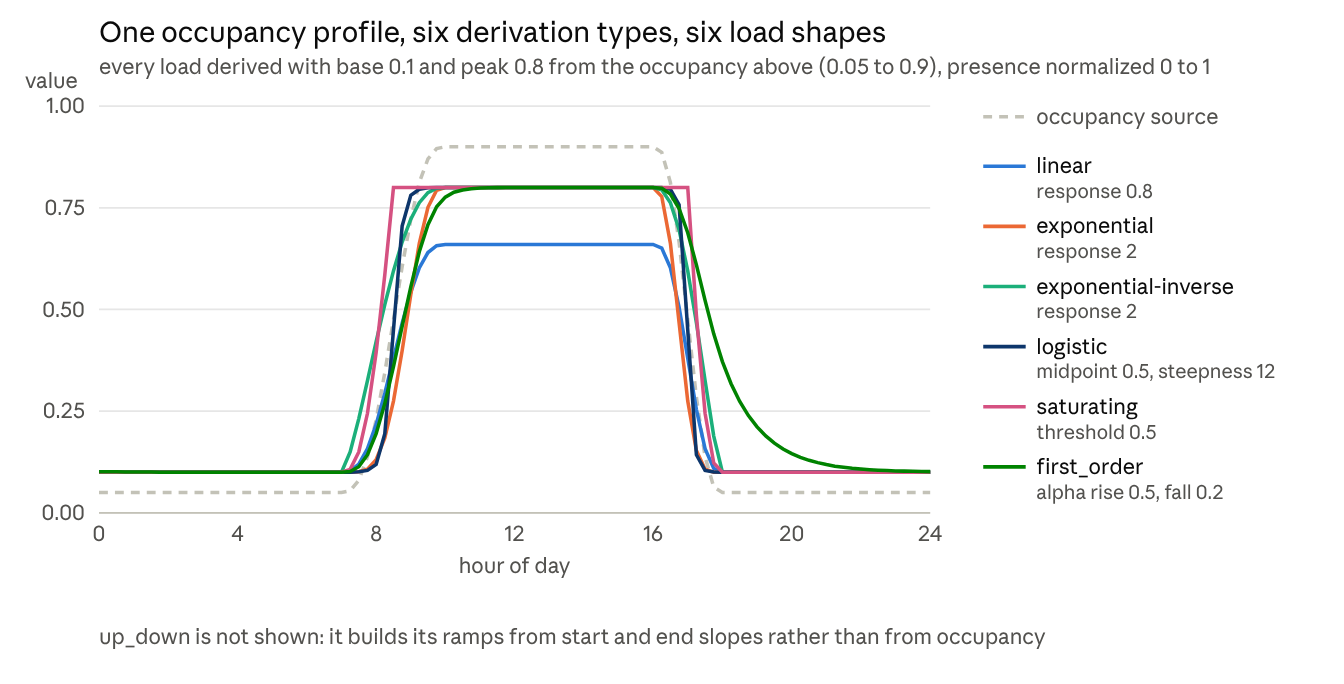
\includegraphics[width=0.9\textwidth]{figures/parametric_derivations.png}
    \caption[Load schedule derivation types]{One occupancy profile and the load schedules derived from it by each derivation type, all with the same base and peak fractions. The derivation type and its parameters are properties of each space type's lighting, equipment, and hot water schedule records.}
    \label{fig:parametric_derivations}
\end{figure}

\begin{figure}
    \centering \includegraphics[width=0.9\textwidth]{figures/ltg_sch_bpr.png}
    \caption[Weekday and weekend lighting base-to-peak ratios by building type]{Weekday and weekend lighting base-to-peak ratios by building type. Base-to-peak ratio is on the x-axis, and fraction of the stock is on the y-axis.}
    \label{fig:ltg_bpr}
\end{figure}

\begin{figure}
    \centering \includegraphics[width=1.0\textwidth]{figures/interior_lighting_eflh.png}
    \caption[Average interior lighting equivalent full load hours by building type]{Average interior lighting equivalent full load hours by building type.}
    \label{fig:interior_lighting_eflh}
\end{figure}

\subsection{Exterior Lighting}
Exterior lighting is all outdoor lighting at the building site, including lighting for parking, walkways, doorways, canopies, building facades, signage, and landscaping.

\subsubsection{Parking Area Lighting}
Parking area lighting accounts for the majority of exterior lighting in the stock \citep{doe2015lmc}. Parking lighting is calculated as the parking area times the installed lighting power per unit of parking area. Parking area is based on the estimated number of parking spots per student for schools, per unit for hotels, per bed for hospitals, and per building floor area for all other building types.  Parking spots are assumed to be 405 ft$^2$. Table \ref{tab:parking} details these assumptions.

Lighting power for a given parking area is determined from the 2015 U.S. Lighting Market Characterization report, which assumes an average of 216 Watts (W) per parking lighting system, or 0.0410 W/ft\textsuperscript{2} (per equation \ref{ext_light_eqn}). Base parking lighting power allowance values for each vintage were reduced by a calculated factor such that the building-count weighted parking lighting power density came out to the 0.0410 W/ft\textsuperscript{2} target.  Note that this calculation is from 2015, so it overestimates the amount of exterior lighting in the stock, which has been changing over to use LEDs. The values for each vintage are shown in Table~\ref{tab:exterior_lighting_power}.
Lighting power for building facades is based on perimeter length and the average of perimeter lighting based on building type from the 4th Commercial Building Stock Assessment from the Northwest Energy Efficiency Alliance (NEEA) \citep{neea2019cbsa}.

\begin{align}
\label{ext_light_eqn}
LPD = \left(\frac{216\,W}{\text{lighting system}}\right) \cdot \left(\frac{1\,\text{lighting system}}{13\,\text{parking spots}}\right) \cdot \left(\frac{1\,\text{parking spot}}{405\,\text{ft}^2}\right) = 0.0410\,W/\text{ft}^2
\end{align}


\subsubsection{Other Exterior Lighting}
Non-parking exterior lighting is determined by the exterior lighting allowance specified in ASHRAE 90.1 for exterior lighting zone 3 (All Other Areas). Length and area estimates are determined from the values in Table \ref{tab:entryways}. The building facade area is calculated from the model as the ground floor exterior wall area. The lighting power allowance is matched to the 90.1 code for each vintage. The exterior lighting power allowances are shown in Table~\ref{tab:exterior_lighting_power}. Note that although 90.1 includes exterior lighting, the only forms of exterior lighting included in ComStock are parking areas, building facades, main entry doors, other doors, drive through windows, entry canopies, and emergency canopies. Notably, ComStock does not include lighting for exterior signage.

\section{Plug and Process Loads}
\label{sec:plug_and_process_loads}

Plug and process loads (PPLs) are all electrical or gas building loads that do not fall under lighting, heating, cooling, ventilation, or water heating. As lighting and HVAC equipment becomes more efficient, PPLs represent an increasing percentage of commercial building energy consumption---up to 50\% in high-performance buildings. This section describes how electric equipment, gas equipment, data centers, elevators, and kitchen equipment are modeled in ComStock. 

\subsection{Electric Equipment}

Electric equipment is a broad category that encompasses any type of load that is powered by an AC outlet. This can include computers, monitors, printers, kitchen or bathroom appliances, laundry equipment, phone chargers, and more. Because there are so many types of electric equipment, ComStock does not model each technology separately, but instead uses an equipment power density (EPD) value for each space type, in watts per square foot. 

The EPDs are a property of the space type. Each space type names an equipment category, and the equipment data carries one or more rows for that category. Where the source data distinguishes the building type the space is in---a classroom in a primary school carries less plug load than one in an office building, and a dining room in a hotel more than one in a school---the row matching the model's primary building type is used; where the data does not distinguish, a single row applies to every building type; and a space type with no row for its building type uses the median across the building types that have one. The values derive from the DOE prototype buildings, with the adjustments made during the end-use load profiles calibration process carried into the data. Using end-use-level data provided by two industry sources for a variety of building types, we increased or decreased some EPD assumptions to better reflect the actual building data. Building types that were affected by the EPD adjustments included Full Service Restaurant (FullServiceRestaurant), Primary School (PrimarySchool), Quick Service Restaurant (QuickServiceRestaurant), Retail (Retail), Secondary School (SecondarySchool), and Strip Mall (StripMall).

Equipment power density does not vary with the building's template. Plug and process loads describe how a space is used rather than what it was legal to install when the building was built, and the typical data is therefore vintage-agnostic; the interior equipment template continues to govern only the efficiency of the equipment that the standards data describes. The EPDs in the ComStock model for each space type, and the building type rows where they differ, are shown in Table~\ref{tab:epds}.


\subsection{Gas Equipment}

Gas equipment refers to any natural gas-powered interior equipment that is not used for space heating or water heating. Similar to electric equipment, there are many different types of gas equipment, so ComStock does not model each technology individually, but rather uses a gas intensity in BTU per hour per square foot, keyed on the space type in the same way as electric equipment. Gas kitchen equipment makes up the majority of the gas equipment modeled in ComStock. Kitchen equipment is discussed separately in Section~\ref{sec:kitchen_equipment}; the kitchen values in the data are placeholders that the kitchen equipment measure replaces with counted appliances. Outside kitchens, only the laundry and operating room space types carry gas equipment. The values used are shown in Table~\ref{tab:gas_equip}.

\begin{table}[h!]
\scriptsize
\centering
\caption[Gas Equipment Power Density]{Gas equipment power density (Btu/hr-ft\textsuperscript{2}) by space type. Kitchen (food preparation) values are the placeholder loads that the kitchen equipment measure replaces with counted appliances, as described in Section~\ref{sec:kitchen_equipment}.}
\label{tab:gas_equip}
\begin{tabular}{|p{2.2in}|p{1.3in}|r|r|r|r|}
\hline
\textbf{Space Type} & \textbf{Building Type} & \textbf{Btu/hr-ft\textsuperscript{2}} & \textbf{Radiant} & \textbf{Latent} & \textbf{Lost} \\ \hline
food preparation & FullServiceRestaurant & 205.8 & 0.2 & 0.1 & 0.7 \\ \hline
 & Hospital & 51.2 & 0.5 & 0 & 0 \\ \hline
 & LargeHotel & 767 & 0.2 & 0.1 & 0.7 \\ \hline
 & QuickServiceRestaurant & 250.9 & 0.2 & 0.1 & 0.7 \\ \hline
 & SuperMarket & 8.5 & 0.2 & 0.1 & 0.7 \\ \hline
food preparation - deli/bakery & any & 100 & 0.2 & 0.1 & 0.7 \\ \hline
food preparation - primary school & any & 453.7 & 0.2 & 0.1 & 0.7 \\ \hline
food preparation - secondary school & any & 532.1 & 0.2 & 0.1 & 0.7 \\ \hline
laundry/washing & LargeHotel & 170 & 0.5 & 0 & 0 \\ \hline
 & SmallHotel & 129.9 & 0.2 & 0 & 0 \\ \hline
laundry/washing - coin-operated laundries & LargeHotel & 170 & 0.5 & 0 & 0 \\ \hline
 & SmallHotel & 129.9 & 0.2 & 0 & 0 \\ \hline
operating room & any & 23.9 & 0 & 0 & 0.5 \\ \hline
\end{tabular}
\end{table}


Gas laundry equipment, in the laundry space types of large and small hotels, represents gas clothes dryers, which are common in commercial drying applications. In operating rooms, in hospitals and outpatient buildings, a small amount of gas equipment represents steam sterilizers or autoclaves, which are used for sterilization during surgical procedures.

\subsection{Data Centers}

Data centers are a high-intensity type of PPL that house IT and computing equipment. Large standalone data centers are not currently modeled in ComStock, but this building type may be added in the future. Instead, ComStock models data centers as a space type within large and medium office buildings. This is meant to represent an IT closet or high-performance computer that is located within an office building and used by a business or organization. 

Data centers are represented by two space types---a high-ITE data center and a low-ITE data center. The high-ITE space type represents the main computer room and has an equipment power density of 45 W/ft\textsuperscript{2}, approximately 20--50 times the equipment load of most other space types \citep{osti_1129366}; the low-ITE space type represents the IT closets and support space around it at a much lower density. The equipment power densities of both are listed in Table~\ref{tab:epds}, and the fraction of floor area each occupies in the office definitions is listed in Table~\ref{tab:space_type_ratios_all}.

In the DOE large office prototype model, the data center represents 2.5\% of the total floor area. The medium office prototype model does not contain a data center space type. If we used the exact space type ratios from the prototype models for ComStock, all large offices would contain a data center, but no medium or small offices would contain this space type. In reality, not all office buildings contain data centers, and they can be present in offices of different sizes. Therefore, ComStock models data centers in a portion of large and medium office buildings, through building subtypes with and without the data center space types. To determine these distributions, we used CBECS 2012 data to understand how prevalent data centers are in office buildings of different sizes. In addition, we used CBECS responses to determine what percent of a typical office building's floor area is dedicated to the data center. From this analysis, we decided that 38\% of large offices and 20\% of medium offices should contain data centers. We also determined that data centers are uncommon in small offices; therefore, there is no data center space type in the small office models.

Data centers follow a very different schedule than the rest of a building's plug and process loads. This type of IT equipment often runs 24 hours a day; therefore, the data center space types have no occupancy and a flat equipment schedule year round, and they are flagged as critical operation so that their zone HVAC equipment runs continuously. The hours of operation and base-to-peak ratio (BPR) adjustments do not affect the data center space types, and no sampled thermostat setpoint or setback is applied to them: they hold the data center setpoints in the space type data around the clock.

\subsection{Elevators}
Elevators are a high power density equipment load present in many commercial buildings. According to the Americans with Disabilities Act (ADA), elevators are required in all commercial buildings with three or more stories, or when the square footage of each floor is more than 3,000 square feet. Although not a requirement, many two-story buildings also contain elevators for accessibility and convenience. Therefore, ComStock includes elevators in all buildings with two or more stories.

Hydraulic elevators are assumed to be installed in buildings with two to six stories, and traction elevators are assumed to be installed in buildings taller than six stories. Hydraulic elevators use a fluid-driven piston to lift the cab, and typically operate at speeds of 150 feet per minute or less. Hydraulic elevators are more affordable and can carry heavier loads, but because of their slow speeds, they are typically only used in buildings up to five stories. For buildings with six or more stories, traction elevators are used because they operate at much higher speeds (up to 500 feet per minute). Traction elevators use a counterweight and pulley system, making them more energy efficient because the motor does not have to move as much weight. The drawbacks, however, include high installation and maintenance costs and limits on cab weights. The motor power is assumed to be 16,055 W for hydraulic elevators and 20,370 W for traction elevators. 

Elevators are modeled as a zone load in EnergyPlus, meaning the elevator equipment load and associated heat gain are attributed to a thermal zone. Elevator load is reported out as part of the electric equipment end use. With hydraulic elevators, the elevator room is typically located in the basement, so the equipment load and heat gain are added to the first floor core zone. With traction elevators, the elevator equipment is located on the roof, so the equipment load and heat gain are added to the top floor core zone.

The number of elevators installed in a ComStock building depends on the building type. For most building types, the number of elevators is based on the floor area. The exceptions are hospitals and hospitality buildings, for which assumptions are based on the number of hospital beds or hotel rooms, respectively. ComStock differentiates between passenger elevators and freight elevators in order to properly capture the elevator load in certain building types with industrial or service elevators. Passenger elevators are modeled in all building types, whereas freight elevators are only modeled in hospital, large hotel, large office, and warehouse buildings. The assumptions for the number of passenger and freight elevators modeled by building type are shown in Tables ~\ref{tab:passenger_elevators} and ~\ref{tab:freight_elevators}.

The equipment schedule for elevators is irregular and unpredictable. Therefore, this load does not follow the typical plug load schedule for its associated space type. We decided to approximate an elevator's schedule by relating it to the number of people who are entering or exiting the building at each time step---in other words, the derivative of the occupancy schedule of the building. We also made assumptions regarding the number of people per elevator ride (five), the amount of time per ride (calculated from the elevator speed and number of stories), and the amount of inter-floor traffic that is not captured by the change in building occupancy (added a factor of 1.2x). Elevator data and metrics like this are not commonly measured or available, so these assumptions are based primarily on engineering judgment. 

From these calculations and assumptions, we derived an elevator schedule for each building type and each day of the week. An example of the elevator schedule for medium offices is shown in Figure~\ref{fig:medium_office_elevator_schedule} for weekdays, Saturdays, and Sundays. On weekdays, the most elevator traffic occurs at the beginning and end of the day, when people are coming in or leaving work for the day. There is also significant traffic during the lunch hour, as some people choose to leave the building for lunch. At all other times during the workday, the elevator load is approximately 40\% of the total load to account for inter-floor traffic and minimal change in the total building occupancy. For some buildings, the occupancy schedules are reduced on Saturdays and include no occupancy on Sundays, which is reflected in the elevator schedule. 

\begin{figure}[ht!]
    \centering 
    \includegraphics[]{figures/medium_office_elevator.png}
    \caption[Medium office elevator schedule]{Elevator fractional load schedule for medium offices on weekdays, Saturdays, and Sundays.}
    \label{fig:medium_office_elevator_schedule}
\end{figure}

The final aspect of modeling elevators is accounting for lighting and fans inside the elevator. Although these are minimal loads compared to the total elevator energy, they are still modeled in ComStock. The elevator lighting and fans are defined in the model by a total power in watts. These wattage values were calculated based on the number of elevators and the subsystem template in the model, thereby ensuring higher efficiencies for newer lighting and ventilation systems. The elevator lighting and fan schedules are assumed to be at full load at all times when the elevator schedule is greater than 0.

\pagebreak

\subsection{Kitchen Equipment}
\label{sec:kitchen_equipment}
Kitchens are one of the most energy-intensive space types. In ComStock, the kitchen is the food preparation space type, which appears in six building types---FullServiceRestaurant, Hospital, LargeHotel, PrimarySchool, QuickServiceRestaurant, and SecondarySchool---and, as the deli and bakery food preparation space type, in grocery stores. In some building types, namely restaurants, the kitchen space type represents a significant proportion of the floor area. In these cases, kitchen loads have a major impact on the total building EUI. In hotels, hospitals, and schools, the kitchen space type only represents a small fraction of the total floor area. Table~\ref{tab:kitchen_floor_area} shows the percent of the total floor area represented by the kitchen space type for each building type. Strip malls that are sampled with a restaurant fraction (Section~\ref{sec:building_type_meta}) carry the full service restaurant's dining and food preparation space types in that fraction of their floor area, and receive cooking equipment in the same way as a restaurant. The cooking equipment described below is placed in every food preparation space in a model, whichever building type contains it, except the grocery deli and bakery service areas, which hold no primary cooking appliances and keep the gas and electric equipment densities of their space type.

\begin{table}[h!]
\small
\centering
\caption[Kitchen Space Type Percentage of Total Floor Area]{Kitchen (food preparation) space type percentage of total floor area}
\label{tab:kitchen_floor_area}
\begin{tabular}{|l|l|l|}
\hline
\textbf{Building Type} & \textbf{Space Type} & \textbf{Percentage of Total Floor Area} \\ \hline
Full Service Restaurant & food preparation & 27.3\% \\ \hline
Hospital & food preparation & 4.1\% \\ \hline
Large Hotel & food preparation & 0.9\% \\ \hline
Primary School & food preparation - primary school & 2.4\% \\ \hline
Quick Service Restaurant & food preparation & 50\% \\ \hline
Secondary School & food preparation - secondary school & 1.1\% \\ \hline
Grocery & food preparation - deli/bakery & 5\% \\ \hline
\end{tabular}
\end{table}


Commercial building energy modeling often assumes an energy intensity per area for cooking equipment, like what is used in the DOE prototype buildings (\cite{qsr_50pct_svs}). However, applying these power densities directly to the various building sizes in ComStock assumes cooking loads scale linearly with kitchen square footage, which does not necessarily represent reality (\cite{eia2012cbecs},~\cite{qsr_50pct_svs}). Further, it does not allow for straightforward analysis of specific cooking equipment since it is represented by a single aggregate load. However, little information exists regarding representative equipment-specific modeling of cooking appliances, as well as how cooking equipment scales with building area. The CBECS survey does provide some level of guidance for area-based intensity as they disaggregate cooking energy consumption separately and provide building area for their samples, but this end use energy consumption data is derived using statistical means from monthly billing data rather than directly measured making it less reliable (\cite{eia2012cbecs},~\cite{qsr_50pct_svs}).


ComStock uses published data to create representative probability distributions of commercial cooking equipment counts, by building type, for both gas and electric appliances. Additionally, the equipment distributions are scaled by area to represent the non-linear scaling suggested in the literature. Although other building types likely include some degree of cooking equipment as well, such as larger offices (\cite{eia2012cbecs}), the current implementation of ComStock only includes cooking equipment in the previously-mentioned six building types plus quick service restaurants found in strip malls. 

Commercial kitchens can contain electric or gas cooking equipment, or a mix of both. The prevalence of gas and electric fuel types for each equipment type used in ComStock are derived from a DOE study (\cite{goetzler_commercial_appliances}). ComStock requires rated input power values and fractions of radiant, latent, and lost heat for gas and electric kitchen equipment. These values are primarily derived from the ASHRAE Fundamentals Handbook (\cite{ashrae2017}) after comparisons with other kitchen equipment studies and commercially available products. More details about how these values were determined can be found in the End Use Savings Shapes documentation (\cite{nrel89130}).The assumptions used in ComStock for prevalence, rated input power, and fractions radiant, latent, and lost for gas and electric appliances are shown in Table~\ref{tab:kitchen_prev_and_power}. 

\input{tables/kitchen_prev_and_power}

Kitchens in ComStock models are assigned a quantity of each equipment type. These can be found in the ComStock metadata files for each model. Equipment quantities are assigned using probability distribtuions with dependencies on building type and floor area by food service and building type. The quantities used in the probability distributions are determined using an older dataset of equipment counts per restaurant type combined with the prevalence of the restaurant type (\cite{com_food_service_equip}). The restaurant types were mapped to ComStock building types. This is summarized in Tables~\ref{tab:kitchen_cook_counts}. Unfortunately, little data of this type was found in literature, so this older source was ultimately used for equipment counts. However, even with changes in culinary trends, it is not expected that counts of equipment types in a restaurant would have changed drastically over the past few decades. Additionally, a “None” restaurant type was created for schools, with a prevalence determined by the fraction of schools in CBECS that have kitchens (\cite{eia2012cbecs}).

This workflow also includes modifiers to the equipment counts shown in Table~\ref{tab:kitchen_cook_counts} to scale equipment count for different kitchen sizes. As mentioned previously, it is not expected that equipment scales linearly with kitchen size, but there is little information in the literature to suggest appropriate scaling (\cite{qsr_50pct_svs}). To account for equipment count scaling, we assume most typically-sized kitchens will have the same quantity of equipment. However, especially small and large kitchens will include scaling factors to account for very large changes in kitchen area that would likely correlate to higher/lower meals served. These factors were determined using engineering judgment and are summarized in Figure~\ref{fig:cooking_equipment_count_scaling_factors_by_building_type_and_area}. Additional scaling factors beyond those shown in Figure~\ref{fig:cooking_equipment_count_scaling_factors_by_building_type_and_area} were applied to Quick Service Restaurants and Full Service Restaurants below 10,000 square feet, as the initial scaling factors resulted in unrealistically high EUIs for very small restaurants. The following supplemental scaling factors were applied to equipment counts:
\begin{itemize}
\item Full Service Restaurants (all restaurant types): \\
    \begin{itemize}
    \item Under 5,000 square feet: equipment counts reduced by an additional 50\% \\
    \item Between 5,000 and 10,000 square feet: equipment counts reduced by an additional 30\% \\
    \end{itemize}
\item Quick Service Restaurants (all restaurant types): \\
    \begin{itemize}
    \item Under 5,000 square feet: equipment counts reduced by an additional 10\% \\
    \item Between 5,000 and 10,000 square feet: equipment counts reduced by an additional 50\%. \\
    \end{itemize}
\end{itemize}

In summary, ComStock determines quantity and fuel type of cooking equipment based on sampling our probability distributions. A restaurant type is sampled for each model as per the prevenances shown by building type in Table~\ref{tab:kitchen_cook_counts}. This yields the corresponding equipment counts for the restaurant type shown in Table~\ref{tab:kitchen_cook_counts}, with square footage modifiers applied based on building size and type. Next, the equipment fuel type is sampled as per the prevalence shown in Table~\ref{tab:kitchen_prev_and_power} for each piece of equipment. Combined, this yields quantities of gas and electric cooking equipment for each ComStock sample. Note that kitchen spaces in ComStock additionally include some prevalence of electric load to account for non-major electrical appliances such as microwaves, heating lamps, toasters, coffee machines, electric kettles, etc. Additionally, the current implementation of cooking equipment in ComStock utilizes the same schedule for each equipment type. Future work could include implementing equipment-specific schedules for the various equipment types, which may better represent reality.


\begin{figure}[ht!] \centering 
    \includegraphics[
        page={1},
        %trim={1cm 18.3cm 1cm 1cm}, clip, % L B R T
        width=\textwidth]{figures/kitchen_equipment_count_scaling.png}
    \caption[Cooking equipment count scaling factors by building type and area]{Cooking equipment count scaling factors by building type and area.}
    \label{fig:cooking_equipment_count_scaling_factors_by_building_type_and_area}
\end{figure}

\section{Service Water Heating}

Service water heating (SWH) includes all water heating usage other than space heating and process requirements. This includes general water heating for uses such as sink faucets and showers, but also building-type-specific uses like commercial dish washing and laundry. This section describes how SWH equipment, fuel type, and usage is incorporated into ComStock models.

\subsection{Service Water Heating Fuel Type}
\label{sec:SWH_Fuel_Type}

It would be logical to assume that the SWH system in a building would use the same fuel as the space heating system. An examination of the CBECS 2012 data \citep{eia2012cbecs} shows that this is the most common case, but it is not always true. In particular, it appears that building types that have large SWH loads, such as hotels and hospitals, are much more likely to use natural gas for SWH, regardless of what their space heating fuel is, presumably because of fuel cost differences. In contrast, building types with low SWH loads are more likely to use electricity for SWH, presumably because of the ease and cost of running wiring compared to installing natural gas piping.

To represent this variability, we used the CBECS 2012 data to create a distribution of SWH fuels for each combination of space heating fuel and building type. The resulting distribution of floor area served by various SWH fuels is shown in Figure \ref{fig:swh_fuel_dist}. As described in Section \ref{sec:HVAC_System_Type_Heating_Fuel_Type}, the prevalence of different space heating fuel varies considerably by county. Because the service water heating fuel depends on the space heating fuel, the probabilities at a stock level are heavily skewed toward the more common space heating fuels, as shown in Figure \ref{fig:swh_fuel_area}.

\begin{figure}[ht!]
  \centering
  \includegraphics[width=\textwidth]{figures/swh_fuel_dist.png}
  \caption[Distribution of service water heating fuel by space heating fuel and building type]{Area-weighted distribution of service water heating fuel by space heating fuel and building type.}
  \label{fig:swh_fuel_dist}
\end{figure}

\begin{figure}[ht!]
  \centering
  \includegraphics[width=\textwidth]{figures/swh_fuel_area.png}
  \caption[Floor area served by each service water heating fuel by space heating fuel and building type]{Floor area served by each service water heating fuel by space heating fuel and building type.}
  \label{fig:swh_fuel_area}
\end{figure}

\subsection{Service Water Heating Usage}
\label{sec:swh_usage}

Hot water use is a property of what happens in a space, not of the building that contains it, so SWH draws are defined per space type. Each space type that uses hot water resolves to a water use equipment record that lists one or more draws, each with a peak flow rate per square foot of the space's floor area, the mixed water temperature delivered at the fixture (110\textdegree F for hand washing and showers, 120\textdegree F for general kitchen use, 140\textdegree F for laundry, 180\textdegree F for dish sanitizing), the sensible and latent fractions of the draw that enter the space, and the type of loop that serves the draw. The records were carried over from the DOE prototype and reference building models and the DEER prototypes, with each prototype space type crosswalked onto its space type name so that exactly one record owns each space type. Table~\ref{tab:swh_flow_rates} lists the draws for every space type that uses hot water.

Because one kitchen record cannot describe both a restaurant kitchen and a hospital kitchen---the restaurant draws roughly six times as much hot water per square foot---the building type definitions (Section~\ref{sec:building_spec}) override the draw where a building type uses a space differently from the generic type record. Restaurant, hotel, and hospital kitchens, outpatient treatment rooms, and hotel guest rooms carry such overrides, and they are listed alongside the stock records in Table~\ref{tab:swh_flow_rates}. An override states only the fields it changes; a draw it sets to zero is not created.

Each draw is placed in every space of its space type and sized on that space's floor area. SWH usage for a given time step is the draw's peak flow rate multiplied by the usage fraction schedule for the time step. The usage fraction schedule is the hot water equipment schedule of the space type's parametric schedule set (Section~\ref{sec:parametric_schedules}), derived from the space type's occupancy schedule in the same way as its lighting and equipment schedules, so hot water draws follow the building's sampled hours of operation and the space type's own daily pattern. Space types with no hot water equipment schedule in their set draw no hot water.

\subsection{Service Water Heating System Type}

The loop type of each draw determines how it is served. Draws of the ``Shared'' type are connected to a single building service water loop with one storage water heater, sized on every draw it serves. The building water heater is a storage tank style heater, either fuel combustion (natural gas, fuel oil, or propane) or electric resistance, as discussed in Section~\ref{sec:SWH_Fuel_Type}; models with district heating as the fuel type receive hot water from off-site and include no on-site water heater. ComStock does not currently model instantaneous or heat pump water heaters. Offices, primary schools, outpatient buildings, hospitals, hotels, and full service restaurants are modeled with a recirculating loop and pump; other building types have a non-recirculating loop. Piping losses are included on the building loop.

Draws of the ``One Per Space'' type, which represent the point-of-use heaters under a restroom sink or in a tenant space, are served by a dedicated electric heater in the space, sized to that space's draws with a minimum under-counter tank size and no distribution piping. A point-of-use loop serving a multiplied zone serves every copy of the space.

Dish sanitizing in food preparation space types is served by a booster water heater. The booster draw is placed on its own 180\textdegree F loop whose heat exchanger sits on the demand side of the building loop, so the building water heater preheats every gallon the booster delivers from the mains temperature to 140\textdegree F and the electric resistance booster heater adds only the final rise to 180\textdegree F. The building water heater is sized on the booster draws as well as its own, so that the preheat load is accounted for.

The design temperature of the building water heater is 140\textdegree F, with a 3.6\textdegree F deadband. The booster loop runs slightly above its 180\textdegree F fixture target so that its tank still delivers 180\textdegree F at the low end of its cycling band. The ambient air temperature for tank heat loss is assumed to be 72\textdegree F. No parasitic losses or part load performance modifiers are included at this time.

\subsection{Service Water Heating Efficiencies}

ComStock water heater efficiencies follow the requirements of ASHRAE-90.1. ComStock currently only models non-condensing units, so water heaters with a combustion fuel source are all roughly 80\% efficient, whereas electric resistance water heaters are roughly 100\% efficient. The efficiency parameters used to calculate the exact water heater efficiencies are summarized in Table~\ref{tab:water_heater_eff} based on SWH template, SWH fuel type, and SWH heater capacity.

\section{Heating, Ventilating, Air Conditioning, and Refrigeration}
\label{sec:HVAC_System_Type_Heating_Fuel_Type}

\subsection{HVAC System Heating Fuel Type}

Commercial HVAC equipment can use various heating fuel types, with the most common being natural gas, electricity, propane, fuel oil, and district heating. To reflect the variability of heating fuels in the real building stock, the ComStock workflow creates probability distributions of heating fuel types per building type at the county level. These distributions are used to assign a heating fuel type to each ComStock building model during the sampling process.

The probability distributions are informed by two data sources. First, there are the CBECS 2012 microdata, which include data on heating fuel(s), building type, and census division for the surveyed buildings. This data can be used to produce probability distributions for heating fuel by building type at the census division level. However, several data sources suggest notable variation within census divisions, which indicates that increased granularity may be needed (beyond what CBECS can provide). The heating fuel type probability distributions used in ResStock---which provides data for residential buildings at the county level---were used to add granularity. However, initial comparisons showed discrepancies between the ResStock data and the CBECS data, which is likely due to inherent differences between residential and commercial buildings. This indicated that the ResStock data should not be used directly. To rectify this, the county-level ResStock data were scaled to align with the CBECS data. This preserved the county-level variation in fuel type prevalence provided by the ResStock data, while also preserving the census division totals provided by the CBECS commercial data. District heating values were not available in the ResStock data, so the per-building-type CBECS values were used for all counties in a given census division.

In some cases, filtering down to a specific region and building type in the CBECS data yields very few samples. This can lead to unreliable conclusions for a region. To mitigate this, we took a blended approach, where some fraction of the CBECS region fuel type percentage comes from the regional samples only, and some fraction comes from the national sample for the building type. If more than 15 samples exist for a given building type and region, then 100\% of the fuel type prevalence comes from that specific region. (The threshold of 15 samples was selected baced on engineering judgment to balance process reliability and regional variability.) If there are fewer than 15 samples, the number of samples divided by 15 will be the fraction used for the region, and the remainder will use the national numbers. For example, if a region has only 12 office samples, 80\% (12\//15) of the effective CBECS regional value will come from the CBECS region, and the other 20\% will come from the national CBECS value for the building type. This will cause region/building type combinations with lower sample sizes to have a stronger inheritance of the national characteristics than the regional characteristics when we lack sufficient evidence to support this level of detail.

Some commercial building HVAC systems use multiple fuel types. For example, a VAV system with a gas furnace in the air handling unit and electric resistance coils in the reheat boxes, or a gas furnace DOAS with variable refrigerant flow (VRF) heat pumps serving the zones. This can complicate the categorization of these systems into a single primary fuel type. To address this, we determine the primary heating fuel type for the mixed fuel systems. The primary heating fuel is the heating fuel expected to carry the majority of the heating load. For example, the previously mentioned example of a VAV system with gas heat at the air handler and electric reheat would be classified as an electric-heated system, since the majority of heating for multizone VAV systems usually comes from the reheat. A full list of ComStock HVAC systems and their fuel type categories are shown in Table~\ref{tab:hvac_system_heating_fuel_categories}. Further detail on model HVAC system assignment methodology can be found in Section~\ref{sec:HVAC_System_Type}.

Figure~\ref{fig:fuel_cbecs_v_cstock} compares the prevalence of heating fuel type by stock floor area for CBECS 2012 and ComStock, by building type. In most cases, ComStock closely aligns to the CBECS 2012 values. However, there are some differences between the two sources due to randomness in the sampling process and from the use of other data sources to achieve county-level granularity in fuel type prevalence. The largest difference is in small hotels where ComStock shows 87\% of the floor area using electric heating while CBECS suggest 74\%, an absolute difference of 12\%.

\begin{figure}
  \centering
  \includegraphics[width=1.10\textwidth]{figures/cbecs_comstock_fuel_type_comparison.png}
  \caption[Comparison of heating fuel type prevalence by floor area between CBECS 2012 and ComStock.]{Comparison of heating fuel type prevalence by floor area between CBECS 2012 and ComStock.}
  \label{fig:fuel_cbecs_v_cstock}
\end{figure}

The county-level prevalences of different heating fuel types are shown in Figure~\ref{fig:map_naturalgas} (natural gas), Figure~\ref{fig:map_electricity} (electricity), Figure~\ref{fig:map_fueloil} (fuel oil), Figure~\ref{fig:map_propane} (propane), and Figure~\ref{fig:map_district} (district heating).

\begin{figure}
  \centering
  \includegraphics[width=0.8\textwidth]{figures/map_naturalgas.png}
  \caption[Fraction of ComStock models using natural gas heating/water heating per county]{Fraction of ComStock models using natural gas heating per county.}
  \label{fig:map_naturalgas}
\end{figure}

\begin{figure}
  \centering
  \includegraphics[width=0.8\textwidth]{figures/map_electricity.png}
  \caption[Fraction of ComStock models using electric heating/water heating per county]{Fraction of ComStock models using electric heating per county.}
  \label{fig:map_electricity}
\end{figure}

\begin{figure}
  \centering
  \includegraphics[width=0.8\textwidth]{figures/map_fueloil.png}
  \caption[Fraction of ComStock models using fuel oil heating/water heating per county]{Fraction of ComStock models using fuel oil heating per county.}
  \label{fig:map_fueloil}
\end{figure}

\begin{figure}
  \centering
  \includegraphics[width=0.8\textwidth]{figures/map_propane.png}
  \caption[Fraction of ComStock models using propane heating/water heating per county]{Fraction of ComStock models using propane heating per county.}
  \label{fig:map_propane}
\end{figure}

\begin{figure}
  \centering
  \includegraphics[width=0.8\textwidth]{figures/map_districtheating.png}
  \caption[Fraction of ComStock models using district heating/water heating per county]{Fraction of ComStock models using district heating per county.}
  \label{fig:map_district}
\end{figure}



%figures moved to appendix

\vspace{5mm}
\subsection{HVAC System Types Probability Distributions}
\label{sec:HVAC_System_Type}

Each ComStock model is assigned a comprehensive HVAC system type. The full list of ComStock HVAC system types is shown in Table~\ref{tab:hvac_system_heating_fuel_categories}. HVAC system types are assigned to ComStock models through sampling informed by representative probability distributions. These probability distributions depend on building type, census division, and heating fuel type. For example, the distributions provide the fraction of gas-heated retail buildings in the West North Central Census Division that use each HVAC system type from Table~\ref{tab:hvac_system_heating_fuel_categories}. The probability distributions are derived from CBECS 2012 microdata, which include data on building type, census division, heating fuel type, and HVAC system type.

\input{tables/hvac_system_heating_fuel_categories.tex}

\subsubsection{CBECS HVAC System Type Analysis}

To derive probability distributions of HVAC system types from the CBECS data, we first assigned one of the comprehensive ComStock HVAC system types shown in Table~\ref{tab:hvac_system_heating_fuel_categories} to the CBECS microdata samples. Historically, this analysis was based solely on the CBECS 2012 data set; however, our updated methodology now integrates data from both the CBECS 2012 and CBECS 2018 data sets. To combine these data sources, we apply a weighted average based on the number of samples from each data set to ensure appropriate representation.

CBECS includes questions regarding the primary HVAC system type of the building; however, it also contains dozens of additional questions about HVAC system components, fuel types, and technologies. In several cases, these responses may conflict with one another, making it difficult to derive a deterministic HVAC system type for the CBECS building samples. Interpretation of the numerous HVAC characteristics into a complete HVAC system type needed for energy modeling involves user discretion and judgment. On multiple occasions, the combinations of survey responses related to the HVAC system were questionable, incomplete, or conflicting based on engineering judgment. This could be due to the survey respondent lacking information about the nuances of the building's HVAC system, the survey respondent skipping relevant questions, or the building having multiple system types, perhaps due to various activities in the building or retrofits and expansions over time. Any of these issues could create a combination of equipment for a CBECS sample that would be difficult to translate into a single, comprehensive HVAC system type without firsthand knowledge of the building. Thus, reliably discerning an HVAC system type from the survey questions can be challenging for some of the CBECS samples and requires some degree of assumption.

Based on survey responses, some CBECS samples appear to utilize multiple types of HVAC systems. For example, one sample responded affirmatively to having a chiller, packaged terminal air conditioners (PTACs), heat pumps, and a swamp cooler. However, there is no indication as to the fraction of the building serving each system type in the survey. Additionally, ComStock is not trying to model buildings with several HVAC system types. To address this, we needed to determine prioritization rules when multiple system types for a single CBECS sample appeared to be prevalent. To achieve this, we grouped systems into the following four categories: VAVs, single-zone RTU, DOAS with zone terminal units (e.g., DOAS with heat pumps, VRF), and miscellaneous single-zone equipment.

There were several cases where the assigned HVAC system for a CBECS sample was unlikely given the size and type of the building. For example, only a small percentage of small office buildings would be expected to use large, multi-zone VAV systems. Similarly, only a small percentage of very large office buildings would be expected to use single-zone RTUs or zone terminal equipment with no DOAS. To address this, we introduced "size bins" to our distributions to ensure system types were correctly assigned based on building size. These size bins were incorporated into the sampling methodology, described in Section \ref{chap:3_sampling}, to further refine system type assignments and improve the alignment between system types and building characteristics. Additional heating-only system types were assigned to building zones whose thermostat setpoints (see \ref{section:therm_setpoints}) described heating-only operation. This primarily affected warehouse buildings in California, representing approximately 13\% of the total stock warehouse floor area, which moved from the primary system type to heating-only gas unit heaters or electric baseboard systems, depending on primary heating fuel source.

Overall, we produced 1,162 probability distributions from the combined CBECS 2012 and 2018 HVAC analysis, with dependencies based on building type, size bin, heating fuel, and census region. These distributions are used with the ComStock sampling process, described in Section \ref{chap:3_sampling}, which ensures that HVAC system types are applied to the correct proportion of models. The prevalence of each HVAC system type in ComStock for all building types is shown in Figure~\ref{fig:hvac_sys_type_prevalence} through Figure~\ref{fig:hvac_sys_type_prevalence_warehouse}.

% AP Decided not to show this table as the information is conveyed more usefully in the figures below
% \input{tables/hvac_system_types.tex} % TODO Format table: This may just be too big with the long names
%figures in appendix

\subsection{HVAC System Sizing}

HVAC system design sizing is determined from several EnergyPlus design day sizing runs. Equipment capacity is hardsized, meaning it is explicitly set in the model. Design day conditions come from the same weather location as the weather file. Design days include the annual heating 99.6\% drybulb temperature, annual cooling 0.4\% drybulb temperature, annual cooling 0.4\% wetbulb temperature for cooling towers and evaporative coolers, and monthly 0.4\% drybulb temperature for August, September, and October to account for buildings with solar-gain driven cooling load maximums.

Per ASHRAE 90.1 Appendix G, HVAC systems are oversized by 15\% for cooling and 25\% for heating. Note that sizing results for a model will be impacted by several control properties specific to the model, such as supply air temperature control, thermostat set points, and outdoor ventilation rates, which are described in later sections.

\subsection{Outdoor Air Ventilation Rates}

Commercial buildings require outdoor ventilation air when the building is occupied. The design outdoor air rate for a system is the minimum amount of outdoor air the system must supply while the building is occupied. The amount of outdoor air required for an HVAC system is calculated by the combined needs of the space type(s) served by a system.

ComStock design outdoor air ventilation rates are a property of the space type and the template family. Each space type names its ASHRAE Standard 62.1 ventilation category, and the ventilation data carries, for that category, a flow rate per person and a flow rate per area, and in some cases an air change rate. For buildings whose HVAC template is ASHRAE 90.1-2004 or later, or DEER 2007 or later, the rates are those of ASHRAE Standard 62.1: Ventilation for Acceptable Indoor Air Quality or DEER standard rates, with ASHRAE Standard 170 rates for the health care space types (patient rooms, exam rooms, operating rooms, emergency rooms, imaging, and recovery, which are ventilated by air changes per hour) and no outdoor air for unoccupied support spaces whose ventilation is provided by exhaust. For the DOE Ref and earlier DEER templates, the rates are those the reference building models of that era carried, which drew on ASHRAE Standard 62-1999 and are generally higher per person and lower per area. The rates for every space type are shown in Table~\ref{tab:ventilation_rates}. Combined, these components determine the design outdoor air requirement for each space and its respective HVAC system. The ASHRAE templates sum the per-person and per-area components; the DEER templates take the greater of the two, following the California calculation method. The design outdoor air of a model is therefore determined by its space type composition (Section~\ref{sec:space_type_ratios}) and its HVAC template.

How the design outdoor air is held during operation depends on the HVAC template. Under the ASHRAE 90.1 and DEER templates, multizone VAV systems hold the design minimum outdoor air volume at every supply flow, as an airflow measurement station or a reset damper does. Under the DOE Ref templates, the minimum outdoor air damper of a multizone VAV system is set to its design position at design supply flow and left there, the common control before outdoor airflow measurement and damper reset, so that outdoor air falls with the supply fan at part load. Health care facilities are the exception: a building with air-change ventilated rooms keeps the minimum outdoor air volume at every supply flow under every template, because hospital ventilation was designed and inspected to health facility guidelines that required outside air quantities to remain constant while the system is in operation.

Some ComStock HVAC system types are residential style systems (denoted ``residential'' in Table~\ref{tab:hvac_system_heating_fuel_categories}). These systems do not include ventilation air and are an exception to the aforementioned ASHRAE-62.1 outdoor air methodology. Although commercial buildings all require outdoor ventilation air per code, some commercial buildings in the stock use residential systems without outdoor air. This is reflected in ComStock through the use of these residential system types. ComStock's HVAC system selection methodology is described further in Section~\ref{sec:HVAC_System_Type}.

\begin{center}
\scriptsize
\begin{longtable}{|p{2.1in}|p{1.05in}|p{1.05in}|p{2.1in}|}
\caption[Design Outdoor Air Rates by Space Type]{Design outdoor air rates by space type, as cfm per person / cfm per ft\textsuperscript{2}. The 90.1 column applies to the ASHRAE 90.1-2004 and later and DEER 2007 and later templates; the DOE Ref column applies to the DOE Ref and earlier DEER templates, which carry the ventilation rates of the reference building models of their era. A space type with zero in both columns receives no outdoor air through its ventilation requirement.} \\ \hline
\label{tab:ventilation_rates}
\textbf{Space Type} & \textbf{90.1 Templates (cfm/person / cfm/ft\textsuperscript{2})} & \textbf{DOE Ref Templates (cfm/person / cfm/ft\textsuperscript{2})} & \textbf{Source} \\ \hline
\endfirsthead
\multicolumn{4}{c}{{\bfseries \textit{Continued from previous page}}} \\ \hline
\textbf{Space Type} & \textbf{90.1 Templates} & \textbf{DOE Ref Templates} & \textbf{Source} \\ \hline
\endhead
audience seating - gymnasium - secondary school & 7.5 / 0.06 & 20 / 0 & ASHRAE 62.1, Spectator areas \\ \hline
audience seating - secondary school & 5 / 0.06 & 15 / 0 & ASHRAE 62.1, Auditorium seating area \\ \hline
classroom/lecture/training & 10 / 0.12 & 16.95 / 0 & ASHRAE 62.1, Classrooms (age 9 plus) \\ \hline
classroom/lecture/training - primary school & 10 / 0.12 & 16.95 / 0 & ASHRAE 62.1, Classrooms (age 9 plus) \\ \hline
classroom/lecture/training - secondary school & 10 / 0.12 & 16.95 / 0 & ASHRAE 62.1, Classrooms (age 9 plus) \\ \hline
computer room & 5 / 0.06 & 5 / 0.06 & curated | ASHRAE 62.1-2019 \\ \hline
conference/meeting/multipurpose & 5 / 0.06 & 20 / 0 & ASHRAE 62.1, Conference/meeting \\ \hline
corridor & 0 / 0.06 & 0 / 0.05 & ASHRAE 62.1, Corridors \\ \hline
corridor - hospital & 0 / 0.06 & 0 / 0.05 & ASHRAE 62.1, Corridors \\ \hline
corridor - primary school & 0 / 0.06 & 0 / 0.05 & ASHRAE 62.1, Corridors \\ \hline
corridor - secondary school & 0 / 0.06 & 0 / 0.05 & ASHRAE 62.1, Corridors \\ \hline
datacenter/high ite & 5 / 0.06 & 5 / 0.06 & curated | ASHRAE 62.1-2019 \\ \hline
datacenter/low ite & 5 / 0.06 & 5 / 0.06 & curated | ASHRAE 62.1-2019 \\ \hline
dining & 7.5 / 0.18 & 20 / 0 & ASHRAE 62.1, Restaurant dining rooms \\ \hline
dining - cafeteria/fast food & 7.5 / 0.18 & 20 / 0 & ASHRAE 62.1, Cafeteria/fast-food dining \\ \hline
dining - primary school & 7.5 / 0.18 & 20 / 0 & ASHRAE 62.1, Cafeteria/fast-food dining \\ \hline
dining - secondary school & 7.5 / 0.18 & 20 / 0 & ASHRAE 62.1, Cafeteria/fast-food dining \\ \hline
electrical/mechanical & 0 / 0.06 & 0 / 0.06 & curated | ASHRAE 62.1-2019 \\ \hline
emergency room & 0 / 0 / 2 ACH & 0 / 0 / 2 ACH & curated | ASHRAE 170-2021 \\ \hline
exam/treatment & 0 / 0 / 2 ACH & 0 / 0 / 2 ACH & curated | ASHRAE 170-2021 \\ \hline
exercise area & 20 / 0.06 & 20 / 0 & ASHRAE 62.1, Health club/aerobics room \\ \hline
food preparation & 7.5 / 0.12 & 0 / 0.47 & ASHRAE 62.1, Kitchen (cooking) \\ \hline
food preparation - deli/bakery & 7.5 / 0.12 & 0 / 0.47 & ASHRAE 62.1, Kitchen (cooking) \\ \hline
food preparation - primary school & 7.5 / 0.12 & 0 / 0.47 & ASHRAE 62.1, Kitchen (cooking) \\ \hline
food preparation - secondary school & 7.5 / 0.12 & 0 / 0.47 & ASHRAE 62.1, Kitchen (cooking) \\ \hline
guest room & 5 / 0.06 & 15 / 0 & ASHRAE 62.1, Bedroom/living room \\ \hline
imaging & 0 / 0 / 2 ACH & 0 / 0 / 2 ACH & curated | ASHRAE 170-2021 \\ \hline
laboratory & 10 / 0.18 & 0 / 1.4 & ASHRAE 62.1, Science laboratories \\ \hline
laundry/washing & 5 / 0.12 & 25 / 0 & ASHRAE 62.1, Laundry rooms, central \\ \hline
laundry/washing - coin-operated laundries & 7.5 / 0.12 & 25 / 0 & ASHRAE 62.1, Coin-operated laundries \\ \hline
library - primary school & 5 / 0.12 & 16.95 / 0 & ASHRAE 62.1, Libraries (public assembly) \\ \hline
library - secondary school & 5 / 0.12 & 16.95 / 0 & ASHRAE 62.1, Libraries (public assembly) \\ \hline
lobby & 5 / 0.06 & 15 / 0 & ASHRAE 62.1, Main entry lobbies \\ \hline
lobby - primary school & 5 / 0.06 & 15 / 0 & ASHRAE 62.1, Main entry lobbies \\ \hline
lobby - secondary school & 5 / 0.06 & 15 / 0 & ASHRAE 62.1, Main entry lobbies \\ \hline
locker room & 0 / 0.5 & 0 / 0.5 & curated | ASHRAE 62.1-2019 \\ \hline
lounge/breakroom & 5 / 0.12 & 5 / 0.12 & curated | ASHRAE 62.1-2019 \\ \hline
nurses station & 5 / 0.06 & 20 / 0 & ASHRAE 62.1, Reception areas \\ \hline
office & 5 / 0.06 & 20 / 0 & ASHRAE 62.1, Office space \\ \hline
operating room & 0 / 0 / 4 ACH & 0 / 0 / 4 ACH & curated | ASHRAE 170-2021 \\ \hline
patient room & 0 / 0 / 2 ACH & 0 / 0 / 2 ACH & curated | ASHRAE 170-2021 \\ \hline
physical therapy & 20 / 0.06 & 20 / 0.06 & curated | ASHRAE 62.1-2019 \\ \hline
playing area - primary school & 20 / 0.18 & 20 / 0 & ASHRAE 62.1, Gym, sports arena (play area) \\ \hline
playing area - secondary school & 20 / 0.18 & 20 / 0 & ASHRAE 62.1, Gym, sports arena (play area) \\ \hline
recovery & 0 / 0 / 2 ACH & 0 / 0 / 2 ACH & curated | ASHRAE 170-2021 \\ \hline
restroom & 0 / 0 & 0 / 0 & curated | ASHRAE 62.1-2019 \\ \hline
restroom - primary school & 0 / 0 & 0 / 0 & curated | ASHRAE 62.1-2019 \\ \hline
restroom - secondary school & 0 / 0 & 0 / 0 & curated | ASHRAE 62.1-2019 \\ \hline
retail & 7.5 / 0.12 & 0 / 0.3 & ASHRAE 62.1, Sales (except as below) \\ \hline
retail - mass merchandising & 7.5 / 0.12 & 0 / 0.3 & ASHRAE 62.1, Sales (except as below) \\ \hline
retail - supermarket & 7.5 / 0.06 & 0 / 0.3 & ASHRAE 62.1, Supermarket \\ \hline
shaft & 0 / 0 & 0 / 0 & ASHRAE 62.1, None \\ \hline
stairwell & 0 / 0 & 0 / 0.05 & ASHRAE 62.1, None \\ \hline
storage & 0 / 0.12 & 0 / 0.12 & curated | ASHRAE 62.1-2019 \\ \hline
storage - warehouse - medium to bulky palletized items & 10 / 0.06 & 1 / 0.05 & ASHRAE 62.1, Warehouses \\ \hline
storage - warehouse - smaller hand-carried items & 10 / 0.06 & 1 / 0.05 & ASHRAE 62.1, Warehouses \\ \hline
\end{longtable}
\end{center}


\pagebreak
\subsection{Fan Systems}

Fans are used in all ComStock HVAC systems except those that rely on radiant heat transfer, such as baseboards. Fans induce pressure in the air stream of HVAC equipment, producing the airflow needed for space conditioning and/or outdoor air ventilation.

\subsubsection{Fan Power}

Fan power determines the amount of energy it takes a fan system to provide a certain amount of airflow. The fan power requirements of each HVAC system are a function of the total pressure drop of the air stream that the fan system will need to overcome (e.g., from filters, coils, air ducts) as well as the efficiency of the fan blades and fan motor.

Fan power in ComStock is determined by ASHRAE-90.1 code requirements. ASHRAE-90.1 determines fan power primarily based on the system type. Constant air volume, variable air volume, and unitary zone equipment are all assigned different fan power allowances.

For implementation in ComStock, fan power is determined based on the static pressure of the air delivery system, the efficiencies of the fan/motor system, and the airflow of the system. The static pressure is based on the HVAC system type and the maximum airflow of the system, as shown in Table~\ref{tab:fan_power}. The fan motor efficiencies are a function of the motor size and HVAC code year, as shown in Table~\ref{tab:fan_motor_efficiencies}.

The addition of energy recovery ventilators (ERVs) in HVAC air loops can add additional static pressure to the air system and therefore result in a higher fan power requirement. ComStock accounts for this additional fan power in the ERV wheel power rather than the fan itself; this allows for improved accuracy during ERV bypass modes (where the airflow bypasses the additional static pressure of the ERV system). See Section~\ref{sec:erv} for more information on ComStock ERV systems.

%TODO: VAV fan curves used

\input{tables/fan_power}

\subsubsection{Fan Controls}

This section describes the operation of fan systems during the hours a building is occupied. Details on the operation of fan systems during unoccupied hours are described in Section~\ref{sec:unoccupied_ahu_operation}.

\paragraph{HVAC Systems Providing Outdoor Air}

As required by ASHRAE-90.1, HVAC systems in commercial buildings must constantly provide the minimum design outdoor air flow rates when the building is occupied. HVAC systems in ComStock follow this control requirement. For constant volume systems, the fan system will run continuously at design airflow during occupied hours. For VAV systems, the fan system will run continuously between the minimum and maximum airflow of the system during occupied hours, always ensuring that the total system airflow meets the airflow needs of every zone.

\paragraph{HVAC Systems Not Providing Outdoor Air}

Systems that do not directly provide outdoor air, such as zone-level unitary systems coupled with a DOAS, do not need to run fans continuously. Therefore, these systems are controlled to cycle the fan system on only when required to maintain zone thermostat set points. Otherwise, the fans are allowed to turn off. This is also the control logic for any residential-style system in ComStock that does not provide outdoor air.

\subsubsection{Zone Exhaust Fans}

Space types that are exhausted---kitchens, laundries, restrooms, and imaging rooms---carry an exhaust rate per square foot of floor area in the exhaust data, keyed on the space type (Table~\ref{tab:exhaust_rates}). A zone exhaust fan sized to that rate is added to each zone containing such a space and is available at all times. Kitchen hoods draw half of their makeup air from the adjacent dining space, which is why a kitchen is always sliced next to its dining room in the building geometry (Section~\ref{sec:space_type_ratios}). The building type definitions override an exhaust rate where a building type's use of a space differs from the record: a hospital's imaging rooms, for example, do not carry the outpatient MRI room's exhaust. The exhaust fan energy is reported as part of the fans end use.

\begin{table}[h!]
\scriptsize
\centering
\caption[Zone Exhaust Rates by Space Type]{Zone exhaust rates (cfm per ft\textsuperscript{2} of space floor area) by space type, the prototype record each rate was carried over from, and the building-type overrides applied by the ComStock building type definitions. Kitchen exhaust draws half of its makeup air from the adjacent dining space.}
\label{tab:exhaust_rates}
\begin{tabular}{|p{2.2in}|p{0.8in}|p{1.6in}|p{1.4in}|}
\hline
\textbf{Space Type} & \textbf{Exhaust (cfm/ft\textsuperscript{2})} & \textbf{Carried Over From} & \textbf{Override} \\ \hline
food preparation & 0.7 & FullServiceRestaurant Kitchen & -- \\ \hline
food preparation - deli/bakery & 1.24 & SuperMarket Bakery & -- \\ \hline
food preparation - primary school & 0.7 & PrimarySchool Kitchen & -- \\ \hline
food preparation - secondary school & 0.7 & SecondarySchool Kitchen & -- \\ \hline
imaging & 1 & Outpatient MRI & Hospital: 0 \\ \hline
laundry/washing & 0.7 & LargeHotel Laundry & -- \\ \hline
restroom & 1.14 & SmallHotel PublicRestroom & -- \\ \hline
restroom - primary school & 0.29 & PrimarySchool Restroom & -- \\ \hline
restroom - secondary school & 0.28 & SecondarySchool Restroom & -- \\ \hline
\end{tabular}
\end{table}


\subsection{Pump Systems}

Pumps are used to induce flow in building hydronic loops. This includes heating water loops, cooling water loops, condenser water loops, and ground-source heat pump water loops.
%TODO service water pump loops

\subsubsection{Pump Power}

Pump power is a function of the pressure head of the hydronic loop and the pump efficiency. The pressure heads in ComStock hydronic systems are set to reflect the baseline requirements specified in ASHRAE-90.1, noting that each hydronic loop type has its own specifications. The pressure heads used for the various ComStock hydronic loop types are specified in Table~\ref{tab:pumps}. Primary-only pump configurations use a single hydronic loop system between the boilers/chillers and the heating/cooling coils for space conditioning. A primary-secondary system uses a primary loop for circulating water between the boilers/chillers, and a secondary loop for supplying the the plant fluid to the heating/cooling coils. Pump motor efficiencies are derived using the same motor efficiency lookup tables used for fans (Table~\ref{tab:fan_motor_efficiencies}).

\subsubsection{Pump Controls}

All pumps in ComStock are set to use intermittent controls, meaning that they can cycle off when there is no load present in the loop. Constant volume pumps are controlled to ride the pump curve, as specified by ASHRAE-90.1, whereas variable speed pumps can adjust their speed to modulate flow as needed. Variable speed pumps all have a minimum flow ratio of 0\% in ComStock. This value is likely too low and underestimates pumping energy, as most pump systems can only reduce flow as low as 30\%--50\% in order to maintain proper operation of chillers, boilers, etc. The assignment methodology for variable speed pumps is specified in Table~\ref{tab:pumps}.

\input{tables/pumps}

%TODO: Make sure VAV is correct
%TODO: Add performance curves for VAV pumps

\subsection{Thermostat Set Points} \label{section:therm_setpoints}
Thermostat set points, both heating and cooling, dictate the target indoor temperature range for the HVAC system to satisfy. The cooling thermostat set point will set the upper temperature limit, whereas the heating thermostat set point will set the lower temperature limit.

Thermostat schedules are built per thermal zone from the setpoint data of the space types in the zone. Each space type carries a stock heating setpoint, a cooling setpoint, and an unoccupied setback delta for each (Table~\ref{tab:thermostat_setpoints_space_types}); the setpoint is the temperature the HVAC system must maintain during occupied hours and the setback is the temperature it must maintain during unoccupied hours, with a setback delta of zero meaning the space type holds its setpoint around the clock. The stock values were derived from the thermostat schedules of the prototype building in which each space type is most commonly found, and the record names that building type. The schedule for a zone switches between setpoint and setback at the building's operating start and end times (Section~\ref{sec:hoo}), so the timing of setbacks aligns with the occupancy schedules; a zone that mixes space types takes the most restrictive setpoint of its space types and the setback temperature that keeps it closest to that setpoint. A minimum deadband between heating and cooling setpoints is enforced on every record, by lowering the heating setpoint where necessary.

The sampled setpoints and setbacks described in the rest of this section enter the model as thermostat overrides on the space types of the building (Section~\ref{sec:building_spec}), applied before the schedules are built. A sampled setpoint replaces the stock setpoint of every space type that is heated or cooled at all, and a sampled setback delta replaces the stock setback delta of every space type whose stock record carries a setback; a space type that holds one temperature around the clock, such as a hotel guest room, a patient room, or a data center, keeps doing so. Data center space types receive no sampled setpoint or setback. When a sampled heating setpoint lands within 2\textdegree F of the cooling setpoint it is lowered to leave a deadband. The building type definitions may also carry thermostat overrides of their own; the hospital definition sets every setback delta to zero, so a hospital never sets back.

\subsubsection{Thermostat Set Points Informed by Building Automation System Data}
\label{section:therm_setpoints_bas}

This section outlines the ComStock thermostat set point assignment methodology for the following building types: full service restaurant, large office, medium office, primary school, quick service restaurant, retail standalone, retail strip mall, secondary school, and small office.

All ComStock building types, excluding hospitals, outpatient, warehouses, and hotels, utilize building automation system (BAS) data to inform distributions of thermostat set points. The methodology behind this approach is described in this section. The intent is to include heating and cooling thermostat set point variability between ComStock models to reflect the thermostat set point variability between real buildings. For example, some offices could be expected to set their heating thermostat to 72°F, whereas others might set it to 70°F. The ComStock methodology allows this variation to exist in the models.

Building automation data from three industry-provided private data sources with over 3,700 buildings were used to derive the distributions of thermostat set points that are used to assign set points to the applicable ComStock models. Table~\ref{tab:bas_thermostat_count_by_btype} shows the counts of buildings with thermostat data available in the data set by building type. The data set includes the time series heating and cooling set points that were used to determine the occupied heating and cooling set points for each building. In turn, these were used to create probability distributions of thermostat set points by building type when aggregating across the data set. For building types with less than 25 samples in the data set, the distribution for all building types was used, as smaller sample sizes cannot reliably be extrapolated to represent a population. The resulting heating and cooling probability distributions, per applicable building type, are shown in Figure~\ref{fig:htg_therm_setpoints} and Figure~\ref{fig:clg_therm_setpoints}, respectively. Note that some outliers exist in the data set at very low prevalence, such as offices with heating set points of 61°F. These outliers are incorporated into ComStock models at a similar low prevalence to reflect the wide diversity of commercial buildings.

\input{tables/thermostat_bas_count}

\begin{figure}
    \centering \includegraphics[width=1.0\textwidth]{figures/heating_setpoints.png}
    \caption{Heating thermostat set point (Fahrenheit) distributions per building type.}
    \label{fig:htg_therm_setpoints}
\end{figure}

\begin{figure}
    \centering \includegraphics[width=1.0\textwidth]{figures/cooling_setpoints.png}
    \caption{Cooling thermostat set point (Fahrenheit) distributions per building type.}
    \label{fig:clg_therm_setpoints}
\end{figure}

\pagebreak
\subsubsection{Unoccupied Thermostat Setbacks}

An unoccupied thermostat setback defines the difference in the temperature set point from the occupied thermostat set point, for either heating or cooling, which is used during periods where the building is unoccupied. For example, an office might have an occupied heating set point of 71°F, but an unoccupied thermostat setback of 6°F for when the building is unoccupied, resulting in an unoccupied thermostat set point of 65°F (71°F - 6°F). This setback would be expected to save HVAC energy by relaxing the temperature requirements when there are no occupants in the building. This section describes ComStock's methodology for assigning unoccupied thermostat setback prevalence, as well as the setback temperature delta, for both heating and cooling.

The prevalence of thermostat setbacks in ComStock models is determined by building type using CBECS 2012. Each building type has some fraction of buildings with a thermostat setback, and some fraction without. The CBECS survey does not provide details on thermostat set point and setback temperatures, but it does provide survey responses as to whether heating and cooling setbacks are used, and whether these setbacks are manual. The survey responses are summarized by building type in Figure~\ref{fig:cbecs_therm_setback_summary}. However, it seems likely that many respondents who claim to implement manual setbacks do not reliably do so; we made a conservative assumption that only 20\% of manual setbacks would be counted as reliably practicing thermostat setbacks (manually adjusting the thermostat every night before leaving and every morning upon entering). The fraction of ComStock models that include thermostat setbacks is shown in Table~\ref{tab:thermostat_setback_prev}. Note that the timing of the thermostat setbacks coincides with the assigned hours of operation for a specific model, the methodology for which is described in Section~\ref{sec:hoo}.

\medskip
\input{tables/thermostat_setback_prev}

\subsubsection{Unoccupied Thermostat Setbacks Informed by Building Automation System Data}

The method for determining the magnitude of the temperature setback for buildings with unoccupied temperature setbacks is described in this section. This methodology is used for the following building types: full service restaurant, large office, medium office, primary school, quick service restaurant, retail standalone, retail strip mall, secondary school, small office, and warehouse. In warehouse buildings, this methodology only applies to the office space type within the building.

The magnitudes of the temperature setbacks are determined using the same data sets and methods described in Section~\ref{section:therm_setpoints_bas} for thermostat set points; probability distributions are created for each building type. The relationship between the thermostat set points and the delta setbacks is shown in Figure~\ref{fig:therm_setpoint_setback}. The resulting heating and cooling thermostat delta setback temperature probability distributions, for each applicable building type, are shown in Figure~\ref{fig:therm_heating_setback} and Figure~\ref{fig:therm_cooling_setback}, respectively.

\begin{figure}
    \centering \includegraphics[width=1.0\textwidth]{figures/heating_setbacks.png}
    \caption{Thermostat heating setback delta temperature probability distributions per building type.}
    \label{fig:therm_heating_setback}
\end{figure}

\begin{figure}
    \centering \includegraphics[width=1.0\textwidth]{figures/cooling_setbacks.png}
    \caption{Thermostat cooling setback delta temperature probability distributions per building type.}
    \label{fig:therm_cooling_setback}
\end{figure}

\subsubsection{Thermostat Setpoints Not Informed by Building Automation System Data}
Hospitals, outpatient buildings, small hotels, and large hotels do not sample thermostat setpoints or setbacks from the BAS distributions. Their zones hold the stock setpoints and setbacks of their space types (Table~\ref{tab:thermostat_setpoints_space_types}). Patient rooms, operating rooms, emergency rooms, and hotel guest rooms hold one temperature around the clock; the office, corridor, lobby, restroom, and storage spaces in these buildings carry the office setpoints and setbacks of the stock data, and the exam, imaging, nurses station, and physical therapy spaces carry the outpatient clinic's. A hospital's building type definition sets every setback delta to zero, so no space in a hospital sets back.

\paragraph{Warehouses}

Heating thermostat setpoints for warehouse storage spaces are adjusted from the prototype model defaults in order to better calibrate warehouse energy consumption to the CBECS truth data set, informed by CBECS 2018 \citep{eia2018cbecs} responses to the ``Percent Heated'' and ``Percent Cooled'' questions as well as engineering judgement. Every warehouse samples a heating setpoint of 61\textdegree F, which applies to both the bulk and the fine storage space types in place of the stock values of 45\textdegree F and 60\textdegree F. The storage space types hold their heating setpoint around the clock, so the sampled heating setback delta applies only to the office portion of the warehouse. No cooling setpoint is sampled for warehouses. Bulk storage is not cooled; its stock cooling setpoint is above the temperature at which a space counts as cooled. Fine storage holds a cooling setpoint of 85\textdegree F, and the office portion of warehouses follows the office space type's stock cooling setpoint.

\pagebreak
\subsection{Unoccupied Air Handling Unit Operation}
\label{sec:unoccupied_ahu_operation}

Commercial buildings require constant design outdoor air ventilation rates when the building is occupied per ASHRAE-90.1. For air handling units (AHUs), the outdoor air is generally mixed with the supply air. This requires constant supply fan operation to maintain the outdoor air requirements established by ASHRAE-62.1 \citep{ashrae_62.1_2004}. However, AHUs do not need to provide outdoor ventilation air when the building is unoccupied. Therefore, ASHRAE-90.1 requires outdoor air dampers to close when the building is unoccupied, and to only cycle on supply fans as needed to maintain thermostat set points. This control scheme can have a large impact on energy usage, and data suggests that not all buildings implement these controls in their AHU systems. This section discusses ComStock's methodology for including the prevalence of different unoccupied AHU control schemes observed in real buildings, which follows the methodology used in \cite{unocc_hvac_paper}.

An industry-provided BAS data set of over 5,700 AHUs was used to inform the prevalence of three unoccupied AHU operation modes. The data set includes time series (hourly) BAS variables for ``Occupied Status'' (describes whether the AHU was in an occupied mode for that hour), ``Fan Status'' (describes whether the fan was used for that hour), and ``Ventilation Status'' (describes whether outdoor ventilation air was used for that hour). Counts of AHUs and buildings by building type in the data set are shown in Table~\ref{tab:unnoc_ahu_data_counts}, and the three unoccupied AHU shutdown control schemes are summarized in Table~\ref{tab:unnoc_ahu_schemes}.

The data set suggests that 27\% of AHUs use scheme 1 (least efficient), 50\% of AHUs use scheme 2 (more efficient), and 23\% of AHUs use scheme 3 (most efficient; ASHRAE-90.1 required). The prevalence of the AHU unoccupied control schemes by building type is shown in Table~\ref{tab:unnoc_ahu_scheme_prev}. These probability distributions are used in ComStock sampling to set the fraction of buildings utilizing the discussed control schemes, by building type, for models that use AHU-based HVAC systems. Non-AHU HVAC system types are not applicable to this methodology, nor are building types not listed in Table~\ref{tab:unnoc_ahu_scheme_prev}. Note that building types with less than 25 buildings in the BAS data set (Table~\ref{tab:unnoc_ahu_data_counts}) use the ``All Types'' distribution of the data set at large, as fewer than 25 samples cannot reliably be used to represent a population.

The following building types are not included in the unnocupied air handling unit operation workflow, and utilize default scheduling only: small hotels, large hotels, outpatient, hospitals, primary schools, and secondary schools. The building types may be integrated into this workflow in the future as more data becomes available.

\input{tables/unnoc_ahu_data_counts}
\input{tables/unnoc_ahu_schemes}

\subsection{Demand Control Ventilation}

Demand control ventilation (DCV) acts to reduce outdoor air ventilation during periods of detected low occupancy. Occupancy levels are generally detected through the use of CO\textsubscript{2} sensors located directly in the space or within the HVAC system.

DCV is included in ComStock models when required by the governing ASHRAE-90.1 energy code for the specific spaces/systems in the model. ComStock gathers the necessary criteria for determining DCV requirements and includes DCV functionality only if the space/system requires it. The requirement criteria for DCV include space floor area, space design occupant density, system economizer prevalence, system design outdoor air flow rate, and system energy recovery prevalence. The 90.1 code year for a model is based on the year of the model's last major HVAC replacement. Code year assignment and system turnover assumptions are described further in Section \ref{sec:system_turnover_and_eul}. A summary of the floor area served by a system with DCV is shown in Table~\ref{tab:dcv_prev}. Note that DCV is not required by ASHRAE 90.1 when an HVAC system has an ERV. Because the DCV requirement is evaluated against the occupant density and floor area of the individual spaces a system serves, it depends on the space type composition of the building: an office building is composed of discrete office, conference, lobby, and support space types, so a conference room served by a system that meets the other criteria can trigger DCV where a single blended office space type could not. DCV is not modeled in any of the buildings in California (which use the DEER data set), although this does not align with the newer versions of Title 24. DCV is expected to be implemented in California buildings in the near future.


\subsection{Air-Side Energy Recovery}
\label{sec:erv}

Energy recovery ventilators (ERVs) in AHUs reduce energy consumption by pre-conditioning the incoming outdoor air using the system exhaust air, which reduces the heating and cooling energy required to condition the air. Energy recovery is especially effective in systems serving spaces with high outdoor air ventilation loads.

ERVs are included in ComStock model HVAC systems only when required by the governing energy code for the specific system. This determination is made using OpenStudio-Standards, where the necessary ComStock model properties are gathered to determine whether an ERV is required for each system. These properties include the climate zone, percent outdoor air, and design supply airflow rate, aligning with ASHRAE-90.1 Table 6.5.6.1 for the respective energy code year followed. A summary of the floor area served by systems with energy recovery is shown in Table~\ref{tab:energy_recovery_prev}.

%TODO: Discuss ERV wheel power methodology

\input{tables/energy_recovery_prevalence}

An enthalpy wheel ERV system (rotary) is added to the HVAC systems in ComStock models where an ERV is determined to be required. The effectiveness of the system is 50\% for all conditions, aligning with the requirements of ASHRAE-90.1. Economizer lockout and supply air bypass for temperature control are included. The defrost type is exhaust only, which temporarily bypasses the supply side of the heat exchanger to allow warmer exhaust air to remove frost uninhibited when needed.

\subsection{Air-Side Economizers}

Air-side economizers reduce HVAC cooling energy by increasing the amount of outdoor ventilation air during times when the temperature and/or enthalpy are beneficial for cooling. For example, if the outdoor air temperature is 55°F when the building needs cooling, the HVAC system can increase the amount of outdoor ventilation air being delivered to the space to satisfy some or all of the cooling requirement in place of mechanical cooling.

As described in Section~\ref{sec:system_turnover_and_eul}, we assume that some building systems, including the HVAC system, are replaced over the lifespan of the building. We re-evaluate the requirement for an air-side economizer based on the energy code in force at the time of the latest HVAC system replacement. For buildings outside of CA, energy code requirements were taken from ASHRAE 90.1. For buildings inside CA, the CA energy code requirements were evaluated taken from the CA DEER MASControl3 models \citep{mascontrol3}, where the economizer limits and applicability were found as shown in Table~\ref{tab:econ_lims_mascontrol3} and Table~\ref{tab:econ_applic_mascontrol3}.

\input{tables/econ_lims_mascontrol3}

\input{tables/econ_applic_mascontrol3}

Figure~\ref{fig:economizer_presence} shows the prevalence of economizers (in terms of floor area coverage and contribution to cooling energy) for different subcategories (building type and ventilation system type) of the existing building stock. The percentage of floor area where "economizer availability" is "True" includes the total building area if there is at least one economizer in the building. It does not represent the total floor area served by systems with economizers. While there are buildings that already include economizers in variable air volume (VAV) systems and roof top units (RTU) covering 40\% of the total floor area and 28\% of total electricity used for cooling, the remaining portion of buildings with those system types do not include economizers.

\begin{figure}
  \centering \includegraphics[width=0.7\textwidth]{figures/economizer_presence.png}
  \caption{Presence of air-side economizers in the building stock.}
  \label{fig:economizer_presence}
\end{figure}

Based on a large body of anecdotal evidence from conversations with fault-focused field engineers and a brief review of common current (Trane, Carrier, Daikin) rooftop unit product data sheets \citep{trane_foundation}, \citep{carrier_economiser}, \citep{daikin_rebel}, fixed dry bulb controls are a more common choice than differential dry bulb controls, although manufacturers also offer dual enthalpy (fixed dry bulb + fixed enthalpy) options with the addition of an enthalpy sensor. For this reason, fixed dry bulb controls are assumed for almost all building vintages and climate zones, with the exception being ASHRAE 90.1-2010 and 2013, which prohibited fixed dry bulb economizers in the warmer humid climate zones. These restrictions were lifted in ASHRAE 90.1-2016.

Figure~\ref{fig:economizer_prevalence} shows the comparison of economizer coverage with respect to building floor area between ComStock and estimation from Commercial Buildings Energy Consumption Survey \citep{eia2018cbecs}. Because of how data is structured in CBECS, the floor area shown in these figures represents the entire floor area of the building if any economizer is present in any of the HVAC systems in the building rather than actual floor area covered by HVAC systems with an economizer. Because CBECS data only shows total building area instead of total area covered by the economizers, this comparison helps give a rough estimate of economizers.

\begin{figure}
  \centering \includegraphics[width=0.7\textwidth]{figures/economizer_prevalence.png}
  \caption{Economizer floor area coverage comparing ComStock (left) with CBECS 2018 (right).}
  \label{fig:economizer_prevalence}
\end{figure}

Economizers are well known for frequent faulty operations. There were many efforts in the past to understand fault characteristics in commercial buildings \citep{doi_10_1080_23744731_2021_1898243}, \citep{osti_1889192}, \citep{osti_1829706}, \citep{osti_1457127}. While this evidence is insufficient to reflect all aspects (e.g., prevalence, incidence, intensity, and evolution described in \citep{doi_10_1080_23744731_2021_1898243}) of all faults in the commercial building stock across the country, it is possible to make simplifications for modeling certain fault types based on available data.

Figure~\ref{fig:econ_temp_fault} shows how the first fault is modeled for buildings with economizers. Crowe et al. \citep{osti_1889192} acquired data from AFDD venders that monitored 3,660 AHUs and 7,974 RTUs and reported 31\% of all economizers were experiencing faulty operations. Shoukas et al. \citep{osti_1665808} received data from a clothing retailer and food chain that monitored 1,416 RTUs and reported 60\% of all faults related to economizers were related to economizer not effectively reducing cooling load compared to the theoretical potential. The symptom described as "ineffective economizing" can be due to different faults: damper stuck, damper bias, sensor bias, sensor frozen, inappropriate configuration, etc. A report \citep{seventhwave_rtu} published by Minnesota Department of Commerce Division of Energy Resources monitored 41 RTUs in Minnesota that were installed in many different building types (e.g., office, restaurant, retail, hotel, etc.) and reported the actual changeover temperature setting in the economizer were not configured efficiently (average of 52°F) resulting in missed free cooling opportunity.

Based on this information focusing on different aspects of the fault, a fault measure was developed as shown in Figure~\ref{fig:econ_temp_fault}. The figure includes a description of the fault as well as four different metrics that define the characteristics of a fault. Fault intensity (or severity) is when a fault can have a severity level. For example, if the sensor is drifting, the intensity is the difference between the true value and the biased measured value. Fault prevalence refers to the portion of systems or components with the fault among all systems or components in the sample space (e.g., 30\% of all economizers have the fault). Fault incidence refers to the occurrence rate of a fault for a given system or component over for a given time period (e.g., economizer damper gets stuck once every year). Fault evolution refers to certain faults where the severity naturally changes over time. For example, sensor drift is typically a fault where the severity changes over the course of time. For the incorrect high limit setting described in Figure~\ref{fig:econ_temp_fault}, the fault changes the changeover temperature setting of an economizer to 52°F and applies to 30\% of economizers that use fixed dry-bulb control. Fault incidence and fault evolution were not modeled because these aspects are mostly irrelevant for this fault.

\begin{figure}
  \centering \includegraphics[width=0.7\textwidth]{figures/econ_temp_fault.png}
  \caption{Economizer incorrect changeover temperature setting fault description.}
  \label{fig:econ_temp_fault}
\end{figure}

Figure~\ref{fig:econ_temp_fault_single_model} shows a comparison of simulated operation with and without the fault. As a result, the fault will reduce the changeover (high limit) temperature of the economizer, disabling the economizer even if the outdoor air temperature is favorable (e.g., 52-72°F), thus, losing opportunities for free cooling. The figure shows how the fault impacts the annual cooling energy, how the changepoint temperature changes with fault, and how the transient response changes.

\begin{figure}
  \centering \includegraphics[width=0.7\textwidth]{figures/econ_temp_fault_single_model.png}
  \caption{Economizer incorrect changeover temperature setting fault impact on simulation results.}
  \label{fig:econ_temp_fault_single_model}
\end{figure}

As reported by Heinemeier \citep{heinemeier2014free}, contractors in California stated that 30-40\% of economizers they have worked with were disabled with fully closed dampers. This is often caused by mechanical linkage issues between damper and actuator, where the economizer automatically reverts to the fully closed position as a safety measure. An economizer with a fully closed damper will not draw any fresh outdoor air, causing an air quality issue. Depending on the outdoor air condition (i.e., favorable or not favorable for economizing), it can either reduce or increase energy consumption. Figure~\ref{fig:econ_damper_fault} shows the description of the fault for the economizer outdoor air damper fully closed and stuck. Unlike the fault described in Figure~\ref{fig:econ_temp_fault}, this fault has a bigger impact on air quality and energy and the incidence of the fault is important.

\begin{figure}
  \centering \includegraphics[width=0.7\textwidth]{figures/econ_damper_fault.png}
  \caption{Economizer damper stuck closed fault description.}
  \label{fig:econ_damper_fault}
\end{figure}

Figure~\ref{fig:econ_damper_fault_single_model} shows example simulation results for a building with and without the damper fully closed fault. The fault was imposed once during the entire April period resulting in 1.8\% mechanical load increase. As mentioned previously, the energy impact of the fault can either be increased or decreased energy consumption, and Figure~\ref{fig:econ_damper_fault_single_model}(c) highlights the transition from negative to positive savings when the outdoor air temperature transitions from favorable to unfavorable conditions.

\begin{figure}
  \centering \includegraphics[width=0.7\textwidth]{figures/econ_damper_fault_single_model.png}
  \caption{Economizer damper stuck closed fault impact on simulation results.}
  \label{fig:econ_damper_fault_single_model}
\end{figure}

Although faults (e.g., damper fully closed) are implemented with fixed prevalence (e.g., 35\%), the actual percentage of economizers being faulted (among applicable economizers) is less than the defined prevalence due to implementation limitations. For example, 35\% of randomly selected buildings that include certain HVAC system types (categorized by the air system) are assigned the damper fully closed fault. However, certain portions of these air systems do not have economizers, thus, they cannot have an economizer fault. In other words, the current limitation is that the random selection of faulted economizers is not fully aligned with buildings that actually have economizers. In these cases, we are losing the opportunity for applying faults and decreasing the representation of fault prevalence in final building stock. Newer versions of California's Title 24 energy code requires fault detection and diagnostics (FDD) for economizers which should prevent and mitigate faults. However, ComStock does not reflect the impact of FDD technology, possibly overestimating the impact of faults in buildings with newer HVAC systems in California.

\subsection{Furnaces}

Furnaces are used in a variety of HVAC equipment for space heating through the direct combustion of a fuel. For ComStock models, the fuel type can be natural gas, propane, or fuel oil. The following ComStock system types use furnaces: PSZ-AC with electric coil, PSZ-AC with gas coil, PTAC with electric coil, PTAC with gas coil, residential AC with residential forced air furnace, and residential forced air furnace.

\subsubsection{Furnace Efficiencies}

Furnaces in ComStock are all assumed to be standard, non-condensing types at this time. Rated efficiency assignments are a function of capacity and in-force HVAC template code. The furnace efficiency assignments are summarized in Table~\ref{tab:furnace_eff_assignments}.

\subsubsection{Furnace Performance Modifiers}

Furnaces in ComStock do not use any performance curves, so there is no change in efficiency or capacity as a function of temperature or part load ratio, and therefore no cycling losses. Furthermore, no parasitic fuel losses are included in ComStock furnace models.

\input{tables/furnace_eff_table}

\subsection{Boilers}

Boilers create hot water for heating in buildings. The following ComStock HVAC types use boilers for heating: DOAS with fan coil air-cooled chiller with boiler, DOAS with fan coil chiller with boiler, DOAS with water source heat pumps cooling tower with boiler, PSZ-AC with gas boiler, PTAC with gas boiler, PVAV with gas boiler reheat, VAV air-cooled chiller with gas boiler reheat, and VAV chiller with gas boiler reheat.

\subsubsection{Boiler Efficiencies}
At this time, boiler systems in ComStock are all gas-fired (or other combustible fuels) storage tank non-condensing units. A single boiler is used to meet the hot water load for the entire building. Rated efficiency assignments are a function of the HVAC code year and boiler capacity, mirroring the requirements of ASHRAE-90.1, and are summarized in Table~\ref{tab:boiler_eff_table}.

\subsubsection{Boiler Part Load Efficiencies}
Boiler efficiency at different part load conditions is modeled through an assigned efficiency as a function of a part load ratio (PLR) cubic curve. The output of this curve is multiplied by the full load rated efficiency, providing the effective efficiency of the boiler for each time step. The performance curve assignments for different boiler scenarios are summarized in Table~\ref{tab:boiler_eff_table}. The curve features are shown in Table~\ref{tab:boiler_plr_curve_table}, and the curves are illustrated in Figure~\ref{fig:blr_plr_curves}.

Table~\ref{tab:boiler_eff_table} shows the older DOE reference building templates using a constant efficiency curve for the boiler (``Boiler Constant Efficiency Curve''). Therefore, these boilers do not currently have efficiency modifications at different part load conditions. This likely underestimates cycling losses that boilers experience at lower PLRs, and may underestimate their gas usage. The 90.1 templates for 2004 through 2010 exclusively use a performance curve for boilers with no turndown controls (``Boiler With No Minimum Turndown''). This provides some efficiency loss, as PLR is reduced. For 90.1-2013 and beyond, performance curves for boilers with minimum turndowns (``Boiler With Minimum Turndown'') are added for larger boiler systems. This provides a slight performance improvement compared to boilers with no minimum turndown. All three curves are illustrated in Figure~\ref{fig:blr_plr_curves}.

%NOTE (From Chris): The curves here do not match the prototype building documentation. I do not know where the "from regression of prototype buildings" curves come from.

%NOTE (From Chris): Currently, the boiler curve assignments result in the oldest boilers having the least efficiency degradation at lower part load ratios. This is probably the opposite of what we want. Recommend finding bad performance curves for older boilers.


\subsubsection{Boiler Controls}

ComStock boilers use 180°F hot water loops with flow that leaves the set point modulated, meaning the boiler model internally varies the flow rate so that the temperature leaving the boiler matches a set point. The delta T of the loop is 20°F. %TODO: do we always use constant setpoint, or is outdoor air reset included sometimes?

\input{tables/boiler_efficiency_table}

\subsection{Direct Expansion Cooling}

Standard air-cooled direct expansion (DX) cooling is the most prevalent cooling equipment type in commercial buildings. The following ComStock HVAC system types use DX cooling: PSZ-AC with district hot water, PSZ-AC with electric coil, PSZ-AC with gas boiler, PSZ-AC with gas coil, PSZ-HP, PTAC with electric coil, PTAC with gas boiler, PTAC with gas coil, PTHP
PVAV with PFP boxes, PVAV with district hot water reheat, PVAV with gas boiler reheat, PVAV with gas heat with electric reheat, residential AC with residential forced air furnace.

\subsubsection{DX Cooling Rated Performance}

DX cooling systems are assigned full load and part load efficiencies based on the HVAC code template for the model and the capacity. These assignments are summarized in Table\ref{tab:unitary_dx_efficiencies} (unitary DX) and Table\ref{tab:ptac_efficiencies} (PTAC). These values mirror those found in ASHRAE-90.1 (or those used in the DOE reference buildings for the pre-1980 template).


\subsubsection{DX Cooling Performance Modifiers}

The performance of DX cooling equipment changes based on operating conditions. ComStock DX cooling equipment uses five performance modifier curves to model this behavior. Energy input ratio (EIR) as a function of part load ratio (PLR) describes how the equipment efficiency varies at different load fractions, accounting for equipment cycling (Figure  \ref{fig:dx_eirfplr}). EIR as a function of temperature describes how the equipment efficiency varies based on both the outdoor air dry bulb temperature and the wet bulb temperature of the air entering the cooling coil (Figure \ref{fig:dx_eirft}). EIR as a function of airflow describes how the equipment efficiency varies as a function of the supply airflow fraction (Figure \ref{fig:dx_eirff}). Capacity as a function of temperature describes how the equipment available capacity varies as a function of both the outdoor air dry bulb temperature and the wet bulb temperature of the air entering the cooling coil (Figure \ref{fig:dx_capft}). Lastly, capacity as a function of airflow describes how the equipment available capacity varies as a function of the supply airflow fraction (Figure \ref{fig:dx_capff}). The outputs of the EIR modifiers are multiplied against the nominal EIR at every time step (except for the PLR modifier, which is divided), which provides the effective EIR at each time step. Meanwhile, the outputs of the two capacity modifiers are multiplied against the nominal capacity at every time step, yielding the effective available capacity for the time step.


\subsection{Air-Source Heat Pumps}

Air-source heat pumps (ASHPs) provide electric heating using a reverse vapor compression cycle. This generally provides a higher COP option for electric heating compared to standard electric resistance electric heating. In most cases, ASHPs use the same air-cooled DX system for both DX heating and DX cooling. ASHPs can be split system, packaged units, or through-the-wall packaged terminal heat pumps (PTHP). The following ComStock HVAC systems types use ASHPs: packaged single zone heat pump (PSZ-HP) and PTHP.

ASHP sizing is often based on the design cooling requirements. Because the DX cooling and heating use the same compressor system, the capacities for each are coupled. ASHPs generally have a minimum operating temperature, below which the DX heating is disabled due to lack of capacity and efficiency. To remedy this, backup heating is often included in colder climates, and for any system where the design heating load is higher than the design cooling load. ComStock ASHP sizing follows this methodology: ASHPs are sized to meet the design cooling load, and backup electric heating is added to the system to meet the design heating load when the available DX heating capacity is unavailable or insufficient. The minimum temperature for compressor operation for ComStock heat pump systems is 17°F PTHP and 10°F for PSZ-HP.
\input{tables/ashp_eff}

\subsubsection{ASHP Rated Performance}

ASHPs in ComStock are assigned efficiencies based on ASHRAE-90.1. The assigned efficiencies are based on the template code year, the unit capacity, and the unit type. These assignments are summarized in Table~\ref{tab:ashp_eff}.

\subsubsection{ASHP Performance Modifiers}

Similar to DX cooling equipment, the performance of ASHP equipment changes based on different operating conditions. The curve assignments are shown in Table~\ref{tab:ashp_curves}. ComStock ASHP equipment uses five performance modifier curves to model this behavior. Energy input ratio (EIR) as a function of part load ratio (PLR) describes how the equipment efficiency varies at different load fractions, where the nominal EIR is divided by the output of this curve to account for equipment cycling losses (Figure~\ref{fig:ashp_eirfplr}). EIR as a function of temperature describes how the equipment efficiency varies based on outdoor air dry bulb temperature (Figure~\ref{fig:ashp_eirft}). Figure~\ref{fig:ashp_eirft} illustrates the capacity loss of ASHPs at lower outdoor air temperatures. EIR as a function of airflow describes how the equipment efficiency varies as a function of the supply airflow fraction (Figure~\ref{fig:ashp_eirff}). Capacity as a function of temperature describes how the equipment available capacity varies as a function of outdoor air dry bulb temperature (Figure~\ref{fig:ashp_capff}). Lastly, capacity as a function of airflow describes how the equipment EIR ratio varies as a function of the supply airflow fraction (Figure~\ref{fig:ashp_capff}). The outputs of the EIR modifiers are multiplied against the nominal EIR at every time step (except for the PLR curve output, which is divided), which provides the effective EIR at each time step. Meanwhile, the outputs of the two capacity modifiers are multiplied against the nominal capacity at every time step, yielding the effective available capacity for the time step. The curves described here are primarily derived from the DOE prototype/reference building models.


\subsection{Air-Cooled Chillers}

Air-cooled chillers (ACCs) provide chilled water for building cooling systems and use an air-cooled condenser for heat rejection. Therefore, no condenser water loop is required for ACCs. The following ComStock HVAC types use ACCs: DOAS with fan coil air-cooled chiller with boiler, VAV air-cooled chiller with PFP boxes, VAV air-cooled chiller with district hot water reheat, and VAV air-cooled chiller with gas boiler reheat.

%TODO CHRIS: add in loop temperatures and setpoint managers.
%TODO CHRIS: chiller condenser type fixed in Standards. Update documentation. This removes the scroll chiller curves.

\subsubsection{Air-Cooled Chiller Rated Performance}

ACCs are assigned full load and part load efficiencies based on the HVAC code template for the model and the capacity. These assignments are summarized in Table~\ref{tab:acc_efficiencies}. These values mirror those found in ASHRAE-90.1 (or those used in the DOE reference buildings for the pre-1980 template).

\input{tables/air_cooled_chiller_eff_table}

\subsubsection{Air-Cooled Chiller Performance Modifiers}

ACCs vary in capacity and efficiency under different operating conditions. ComStock uses three curve types to model the variation in performance: capacity as a function of temperature (CAPFT) modifier, EIR as a function of temperature (EIRFT) modifier, and EIR as a function of part load ratio (EIRFPLR) modifier. For each time step, the EIR modifier function outputs are multiplied by the ACC's rated EIR (except for the PLR curve output, which is divided). This provides the realized EIR for the time step. Similarly, the CAPFT modifier function output is multiplied by the ACC's nominal capacity every time step to get the actual available capacity for that time step. The curve assignments are summarized in Table \ref{tab:acc_efficiencies}, and the curve parameters are specified in Table \ref{tab:acc_perf_curves}. The curves are also illustrated in Figure \ref{fig:acc_eir_curves}, Figure \ref{fig:AirCooledChiller2010PathA_funct_curves}, and Figure \ref{fig:ChlrAirRecipQRatio_curves}.

%TODO, BUG: Standards does not specify the "condenser_type" field, so the model chooses the first in the list for the template call. This is why 2013 and beyond models use different performance curves.

\subsection{Water-Cooled Chillers}

Water-cooled chillers (WCCs) provide chilled water for building cooling systems and use a water-cooled condenser for heat rejection. Therefore, a condenser water loop is required for WCCs, generally conditioned by a boiler and cooling tower. The following ComStock HVAC types use WCCs: DOAS with fan coil chiller with baseboard electric, DOAS with fan coil chiller with boiler, DOAS with fan coil chiller with district hot water, VAV chiller with PFP boxes, VAV chiller with district hot water reheat, and VAV chiller with gas boiler reheat.

\subsubsection{Water-Cooled Chiller Rated Performance}

WCCs are assigned full load and part load efficiencies based on the HVAC code template for the model and the capacity. These assignments are summarized in Table~\ref{tab:wcc_eff}. These values mirror those found in ASHRAE-90.1 (or those used in the DOE reference buildings for the pre-1980 template).

\input{tables/wcc_eff}

\subsubsection{Water-Cooled Chiller Performance Modifiers}

WCCs have been shown to vary capacity and efficiency at different operating conditions. ComStock uses three curve types to model the variation in performance: capacity as a function of temperature (CAPFT) modifier, EIR as a function of temperature (EIRFT) modifier, and EIR as a function of part load ratio (EIRFPLR) modifier. For each time step, the EIR modifier function outputs are multiplied by the WCC's rated EIR (except for the PLR curve output, which is divided). This provides the realized EIR for the time step. Similarly, the CAPFT modifier function output is multiplied by the WCC's nominal capacity every time step to get the actual available capacity for that time step. The curve assignments are summarized in Table\ref{tab:wcc_eff}, and the coefficients are shown in Table~\ref{tab:wcc_perf_curves}. Furthermore, the performance curves are illustrated in Figure~\ref{fig:wcc_plr} (EIRFPLR for all chillers), Figure\ref{fig:wcc_WaterCooled_PositiveDisplacement_Chiller_LT150_2010_Modifiers}, and Figure\ref{fig:ChlrAirRecipQRatio_curves}.


\subsection{Cooling Towers}

Cooling towers are an HVAC component used to reject heat from a condenser water loop. The following ComStock HVAC system types use cooling towers: DOAS with fan coil chiller with baseboard electric, DOAS with fan coil chiller with boiler, DOAS with fan coil chiller with district hot water, DOAS with water source heat pumps cooling tower with boiler, VAV chiller with PFP boxes, VAV chiller with district hot water reheat, and VAV chiller with gas boiler reheat.

The cooling tower assumptions used in ComStock are primarily code-driven and are summarized in Table~\ref{tab:cooling_towers_table}.

\input{tables/cooling_towers_table}

\subsection{Water-Source Heat Pumps}

Water-source heat pumps (WSHPs) are an HVAC system type that uses water-to-air heat pumps for space conditioning. These differ from ASHPs in that the condenser side of the heat pumps use water from a condenser water loop as the heat source/sink instead of air. The following ComStock HVAC system type(s) use WSHPs: DOAS with water source heat pumps cooling tower with boiler.

\subsection{Ground-Source Heat Pumps}
Ground-source heat pumps (GSHPs) are WSHP systems that use the ground as the heat sink for the condenser water loop. The temperature of the ground is fairly constant throughout the year, which makes the ground an effective heat sink for the refrigeration cycle. The following ComStock HVAC system type uses GSHPs: DOAS with water source heat pumps with ground source heat pump.

The GSHP model in ComStock uses the ``Plant Component Temperature Source'' with energy management system (EMS) controls to represent the temperature behavior of the ground condenser water loop. The EMS predicts the exit temperature of the ground loop based on the inlet temperature of the loop, where the exit temperature will directly impact the efficiency and capacity of the heat pump system. A warmer exit temperature will generally be beneficial for heating, whereas a colder exit temperature will generally be beneficial for cooling. The exit temperature in ComStock is predicted by a linear interpolation that assumes a +12°F delta temperature at the lowest expected inlet loop temperature of 30°F (42°F loop exit temperature), and a -12°F delta temperature at the highest expected inlet loop temperature of 90°F (78°F loop exit temperature), while ramping linearly in between. The relationship between the inlet loop temperature and the outlet loop temperature is illustrated in Figure~\ref{fig:gshp_loop_temps}. Note that there is no change in the loop temperature at 60°F, as this approach results in a constant ground temperature assumption of 60°F.

\subsection{Refrigeration}
\label{sec:refrigeration}

In ComStock, refrigeration systems refer to the refrigerated cases and walk-ins found in commercial kitchens, grocery stores, and other food service spaces. Small plug-in refrigerators are included in plug and process loads, as described in Section~\ref{sec:plug_and_process_loads}. Refrigeration is modeled in building types where it is a major end use (primary and secondary schools, restaurants, hotels, hospitals, and grocery stores).

\subsubsection{Walk-ins and Case Scaling}
Earlier versions of ComStock used fixed-size walk-in coolers and freezers for each building kitchen zone. This has been replaced with a scaling approach: refrigeration equipment is now sized according to the floor area of the associated space type (such as kitchens, stock rooms, or grocery sales areas). Rather than applying fixed case or walk-in sizes, ComStock uses reference space types to establish a ratio of refrigerated area or case length to total floor area. For example, a reference space type might assume 20{,}000 ft$^2$ of grocery sales area with 400 ft of refrigerated cases; this ratio of case type to floor area is then scaled to the actual space type floor area in the model. This scaling approach is consistent with the best available data sources and has been validated through in-person site visits performed by NREL staff, providing confidence that modeled refrigeration capacities align with real-world practice.

\subsubsection{Technology Level Assignment}
Refrigeration systems are now characterized by probabilistic assignment of technology levels: \textit{old}, \textit{new}, and \textit{advanced}. These levels represent distributions of baseline efficiency as a function of both building vintage and building size. Technology levels influence compressor efficiency, case lighting, fan motors, and defrost cycles. This approach allows ComStock to capture variability in stock performance, from legacy systems to modern ENERGY STAR\textsuperscript{\textregistered}-like equipment~\citep{DOE_TSD_2009,ENERGYSTAR_Refrigeration}.

The assignment of technology levels draws from three TSVs:
\begin{itemize}
    \item \textit{include\_refrigeration\_technology\_level.tsv} flags buildings with refrigeration.
    \item \textit{year\_bin\_of\_last\_refrigeration\_replacement.tsv} assigns the year range of the last major equipment replacement, based on survival curves (see Section~\ref{sec:refrigeration_survival}).
    \item \textit{refrigeration\_technology\_level.tsv} probabilistically assigns equipment efficiency distributions based on year built, replacement year, and building size.
\end{itemize}


Figure~\ref{fig:refrigeration_tech_distribution} illustrates the resulting distribution of refrigeration technology levels by building size and year of last replacement.

\subsubsection{Efficiency Distributions}
Efficiency distributions for refrigeration equipment are derived from DOE Technical Support Documents, ENERGY STAR\textsuperscript{\textregistered} archives, ASHRAE research, and utility/laboratory studies~\citep{DOE_TSD_2009,Fricke2010,CEC_Title20}. Historical data show a clear trend of improvement:
\begin{itemize}
    \item Pre-1990 equipment had very high energy intensities (e.g., 0.3--0.4~kWh/ft$^3$/day for reach-in refrigerators, 2.5--3.0~kWh/ft/day for open vertical cases).
    \item 1990s equipment introduced modest improvements (better insulation, new refrigerants), but performance was still poor by modern standards.
    \item Early 2000s saw the introduction of ENERGY STAR\textsuperscript{\textregistered} criteria and California Title 20 standards, driving significant efficiency gains in reach-ins, freezers, and merchandisers.
    \item By the late 2000s, most new commercial refrigeration equipment met or exceeded federal standards, with widespread adoption of LED case lighting, ECM fan motors, anti-sweat heater controls, and night covers.
\end{itemize}

These historical shipment distributions were mapped to \textit{old}, \textit{new}, and \textit{advanced} efficiency levels using Oak Ridge National Laboratory (ORNL) performance data embedded in OpenStudio Standards. In practice, ComStock samples from these distributions to assign performance characteristics to each refrigeration system. Approximate efficiency values by technology level are summarized in Table~\ref{tab:refrigeration_efficiency_levels}. This ensures the resulting stock reflects both legacy equipment and the adoption of modern efficiency measures over time.

%\usepackage{threeparttable}

\begin{table}[h!]
\centering
\begin{threeparttable}
\caption{Approximate efficiency levels for refrigeration equipment categories (illustrative ranges).}
\label{tab:refrigeration_efficiency_levels}
\begin{tabular}{|p{1.8in}|p{1.2in}|p{1.2in}|p{1.2in}|}
\hline
\textbf{Equipment Category} & \textbf{Old (Legacy / Pre-Standard)} & \textbf{New (Standard-Era Baseline)} & \textbf{Advanced (High Efficiency / ENERGY STAR)} \\ \hline
Reach-in Refrigerators (solid/glass door) & 0.30--0.40 kWh/ft$^3$/day & 0.20--0.30 kWh/ft$^3$/day & 0.15--0.20 kWh/ft$^3$/day \\ \hline
Reach-in Freezers & 0.50--0.60 kWh/ft$^3$/day & 0.40--0.50 kWh/ft$^3$/day & 0.30--0.40 kWh/ft$^3$/day \\ \hline
Vertical Open Display Cases (medium-temp) & 2.3--3.0 kWh/ft/day & 1.8--2.3 kWh/ft/day & 1.2--1.6 kWh/ft/day \\ \hline
Horizontal/Coffin Freezers (low-temp) & 2.0--2.5 kWh/ft/day & 1.5--2.0 kWh/ft/day & 1.0--1.4 kWh/ft/day \\ \hline
Walk-in Coolers (8$\times$8 typical) & 0.07--0.09 kWh/ft$^3$/day & 0.05--0.07 kWh/ft$^3$/day & 0.03--0.05 kWh/ft$^3$/day \\ \hline
Walk-in Freezers (8$\times$8 typical) & 0.14--0.18 kWh/ft$^3$/day & 0.11--0.14 kWh/ft$^3$/day & 0.08--0.11 kWh/ft$^3$/day \\ \hline
\end{tabular}
\begin{tablenotes}
\footnotesize
\item Values represent typical daily energy use intensities under standard test conditions, used to define the ``Old,'' ``New,'' and ``Advanced'' technology levels applied in ComStock. Ranges are derived from DOE Technical Support Documents, ENERGY STAR\textsuperscript{\textregistered} criteria, and ASHRAE/utility research studies, and mapped to OpenStudio Standards performance data.
\end{tablenotes}
\end{threeparttable}
\end{table}


\subsubsection{System Types and Controls}
Refrigeration configurations also vary by building type and size. Large grocery stores almost universally use centralized compressor rack systems serving dozens of cases and walk-ins, while small-format stores rely on self-contained units~\citep{EIA_FoodSales2018}. Efficiency technologies such as floating head pressure control, variable-speed compressors, adaptive defrost, and LED case lighting are incorporated in proportion to their historical and present-day adoption levels. For example:
\begin{itemize}
    \item Floating head pressure control was common by the late 1990s and is standard in modern racks.
    \item Variable-speed compressors and VFD-controlled condenser fans are now standard in new systems.
    \item Adaptive defrost and anti-sweat heater controls are widely adopted in newer or retrofitted equipment.
    \item Medium-temperature case doors, once rare, are now installed in roughly half of all modern supermarkets, reflecting a major retrofit trend.
\end{itemize}

\subsubsection{Summary}
In summary, ComStock’s refrigeration modeling now:
\begin{itemize}
    \item Scales walk-in and case sizes based on space type floor area, validated against site visits and data sources;
    \item Applies survival-based replacement schedules to reflect realistic equipment lifetimes (Section~\ref{sec:refrigeration_survival});
    \item Assigns technology levels probabilistically, capturing distributions of baseline efficiency by vintage and size, based on DOE shipment data mapped to OpenStudio Standards performance levels;
    \item Incorporates adoption of modern refrigeration efficiency measures and retrofit trends.
\end{itemize}

This methodology ensures that ComStock refrigeration energy use better reflects the diversity of U.S. commercial building stock, including both legacy equipment and advanced technologies.

\begin{figure}
    \centering
    \includegraphics[width=0.9\textwidth]{figures/refrigeration_tech_distribution.png}
    \caption{Distribution of refrigeration technology levels (old, new, advanced) by building size and year of last replacement. Based on DOE shipment data mapped to OpenStudio Standards performance levels.}
    \label{fig:refrigeration_tech_distribution}
\end{figure}
\include{4_10_simulation_settings}
\chapter{ComStock Outputs}
ComStock creates a wide array of data that can be analyzed and aggregated to draw conclusions. While it is common to look at how results vary by building type and climate zone, ComStock provides a wide range of outputs not traditionally provided in large-scale analyses, with the hope of providing maximum utility.

Sections \ref{rawsimulationresults} and \ref{dataviewer} describe how to access ComStock outputs. Additionally, the sample building energy models are available at \url{https://data.openei.org/} in the nrel-pds-building-stock data lake. See the README.md file for details.

\section{Energy Consumption by Fuel and End Use}
ComStock provides energy consumption by fuel and end use at both an annual and time-series (typically 15-minute time steps for one year) resolution. Not all combinations of fuels and end uses are found in ComStock. The definitions below describe the fuels and end uses in detail.

ComStock provides modeled energy consumption for the following \textbf{fuels}:

\begin{itemize}
  \item \textbf{Electricity}: This represents the electricity that is delivered to the building through the power grid and consumed on-site. How this electricity is generated depends on the generation mix found on the power grid in the region serving the building. This does not include electricity that is generated through a backup generator.
  \item \textbf{Natural Gas}: This represents the natural gas that is delivered to the building through the natural gas pipeline system and consumed on-site.
  \item \textbf{Propane}: This represents the propane that is delivered to the building in tanks and consumed on-site.
  \item \textbf{Fuel Oil}: This represents the liquid fuel oil that is delivered to the building, stored in tanks, and consumed on-site.
  \item \textbf{Other Fuel}: In some ComStock outputs, propane and fuel oil are combined and reported together as ``other fuel'' due to reporting limitations in the simulation engine. Where this is the case, propane and fuel oil are not reported separately to avoid double-counting.
  \item \textbf{District Heating}: This represents the hot water or steam that is delivered to the building through a district heating piping system and consumed on-site. The quantity of energy consumed represents only the energy extracted from the district heating system by the building; it does not represent the consumption of electricity or natural gas at the district heating plant required to provide heat to the building. In order to capture the energy consumption of the district heating plant, assumptions about distribution heat losses, pumping power, and district heating plant equipment efficiency and controls may be made.
  \item \textbf{District Cooling}: This represents the chilled water that is delivered to the building through a district cooling piping system and consumed on-site. The quantity of energy consumed represents only the energy extracted from the district cooling system by the building; it does not represent the consumption of electricity or natural gas at the district cooling plant required to provide chilled water to the building. In order to capture the energy consumption of the district cooling plant, assumptions about distribution heat gains, pumping power, and district cooling plant equipment efficiency and controls may be made.
\end{itemize}

ComStock provides modeled energy consumption for the following \textbf{end uses} for each applicable fuel:

\begin{itemize}
\item \textbf{Cooling}: This includes all energy consumed by primary cooling equipment such as chillers, direct expansion air conditioners (includes condenser fan energy), and direct expansion heat pumps in cooling mode (includes condenser fan energy). This also includes parasitic energy consumption of the equipment, such as pan heaters, defrost energy, and any energy needed to overcome modeled pipe losses.
\item \textbf{Heating}: This represents all energy consumed by primary heating equipment such as boilers, furnaces, natural gas heating coils, electric resistance strip heating coils, and direct expansion heat pumps in heating mode (includes evaporator fan energy). This also includes parasitic energy consumption of the equipment, such as pilot lights, standby losses, defrost energy, and any energy needed to overcome modeled pipe losses.
\item \textbf{Fans}: This includes all energy consumed by supply fans, return fans, exhaust fans, and kitchen hoods in the building. It excludes the condenser fan energy from direct expansion coils, which is captured in cooling and heating, as described above.
\item \textbf{Pumps}: This includes all energy consumed by pumps for the purpose of moving hot water for heating and service water heating, chilled water for cooling, and condenser water for heat rejection.
\item \textbf{Heat Recovery}: This includes the energy used to turn heat or enthalpy wheels, plus the increased fan energy associated with the increased pressure rise caused by the heat recovery wheels.
\item \textbf{Heat Rejection}: This includes the energy used to run cooling towers and fluid coolers to reject heat from the condenser water loop to the air. As previously noted, condenser fans on direct expansion cooling and heating coils are included in heating and cooling.
\item \textbf{Humidification}: This includes all energy used to purposely increase humidity in the building. Most buildings are assumed not to use humidification.
\item \textbf{Water Systems}: This includes all energy consumed by the primary service hot water supply equipment, such as boilers and water heaters. This also includes parasitic energy consumption of the equipment, such as pilot lights, standby losses, and any energy needed to overcome modeled pipe losses.
\item \textbf{Refrigeration}: This includes all energy used by large refrigeration cases and walk-ins such as those commonly found in grocery stores and large commercial kitchens. Plug-in refrigerators, such as those commonly found in the checkout areas of retail stores, are included in interior equipment.
\item \textbf{Interior Lighting}: This includes all energy used to light the interior of the building, including general lighting, task lighting, accent lighting, and exit lighting.
\item \textbf{Exterior Lighting}: This includes all energy used to light the exterior of the building and the surrounding area, including parking lot lighting, entryway illumination, and wall washing.
\item \textbf{Interior Equipment}: This includes all energy used in the building that was not included in one of the other categories. This covers miscellaneous electric loads such as computers and monitors, large equipment such as elevators, and special-purpose equipment such as data center and IT-closet servers. This is a large and coarse bin, largely because the variety of energy-consuming devices found in buildings is large and little comprehensive data are available.
\end{itemize}

\begin{figure}
    \centering
    \includegraphics
    [width=\textwidth]{figures/Segments_typology.png}
    \caption[Example of ComStock Results]{Example ComStock Results}
    \label{fig:segments_typology}
\end{figure}

\section{Building Characteristics}
In addition to energy consumption data, ComStock outputs include a variety of building input characteristics. Most of these are either direct or indirect inputs to the building model generation workflow. Units for these characteristics are described in the files that accompany the ComStock data sets. Names and descriptions for these characteristics are included in Table \ref{tab:building_input_characteristics}.

\input{tables/building_input_characteristics}
\pagebreak
\section{Building Summary Statistics}
In addition to the building input characteristics, ComStock outputs include a variety of summary statistic information about the building.  These statistics captures building characteristics that result from the complex rules that are applied to HVAC systems after sizing routines and are therefore not easy to discern from the building input characteristics. Units for these outputs are described in the files that accompany the ComStock data sets. Names and descriptions for these summary statistics are included in Table \ref{tab:building_summary_stats}

\section{Greenhouse Gas Emissions Reporting}
ComStock calculates the greenhouse gas emissions from the building stock and savings from measures using both historical and projected emissions data.

\subsection{Electricity Emissions}
\subsubsection{eGRID Historical Emissions}
Historical emissions use the CO\textsubscript{2}-equivalent total output emission rate from EPA's Emissions and Generation Resource Integrated Database (eGRID)\citep{egrid2020}. ComStock results include the historical emissions for 2018, 2019, 2020, and 2021 using eGRID U.S. state and eGRID subregion emissions factors. eGRID regions are similar to Cambium grid regions but not identical. Notably, eGrid separates out New York into upstate, New York City, and Long Island. Cambium uses a whole-state average, and historical emissions use the New York state average instead of the grid region for New York buildings. Historical eGrid emissions rates are an \textit{annual} average multiplied by the total annual electricity use.

\subsubsection{Cambium Projected Emissions}
Projected emissions use data from NREL's Cambium 2022 data set \citep{cambium2022}. Projected emissions consider both the average emissions rate (AER) and the long-run marginal emission rate (LRMER).  LRMER, described in \cite{GAGNON2022103915}, is an estimate of the rate of emissions that would be either induced or avoided by a long-term (i.e., more than several years) change in electrical demand.  LRMER data is levelized over 15 and 30 years\citep{cambium2022}. ComStock results including End Use Savings Shapes round 1 results and earlier projects used emissions factors from the Cambium 2021 data \citep{cambium2021},\citep{lrmer_data2022}.

\subsection{On Site Fossil Fuel Emissions}
Natural gas, propane, and fuel oil emissions use the emission factors in \textit{Table 7.1.2(1) of draft National Average Emission Factors for Household Combustion Fuels} defined in \textit{ANSI/RESNET/ICCC 301-2022 Addendum B-2022 Standard for the Calculation and Labeling of the Energy Performance of Dwelling and Sleeping Units using an Energy Rating Index}. Natural gas emissions include both combustion and pre-combustion emissions (e.g., methane leakage for natural gas).

On-Site Fossil Fuel Emissions Factors:\\
Natural gas: 147.3 lb/MMBtu (228.0 kg/MWh)\\
Propane: 177.8 lb/MMBtu (275.7 kg/MWh)\\
Fuel oil: 195.9 lb/MMBtu (303.2 kg/MWh)\\

\subsection{District Energy Emissions}
District heating and cooling emissions use the emissions factors defined in the August 2024 version of the \textit{Energy Star Portfolio Manager Technical Reference} available at \url{https://portfoliomanager.energystar.gov/pdf/reference/Emissions.pdf}. The district heating emissions factor is the same for both steam and hot water. The district cooling emissions factor assumes district chilled water served by electric driver chillers. The emissions factors were originally sourced from EIA data for district chilled water and the EPA voluntary reporting program for district steam and hot water. These district emissions factors do not include upstream methane leakage. There is considerable variation by location and type of district system, so you may need to scale the results by factors specific to your region or system.

On-Site Fossil Fuel Emissions Factors:\\
District Cooling: 52.70 kg/MMBtu\\
District Heating: 66.40 kg/MMBtu\\

\subsection{Air Pollution from On Site Fossil Fuel Combustion}
ComStock reports annual pollution emissions for NOx, CO, PM, SO2 from on-site combustion of natural gas, propane, and fuel oil. Emission factors are from U.S. EPA \textit{AP-42: Compilation of Air Emissions Factors from Stationary Sources}\citep{epa_ap42}. Natural gas emissions use emissions factors from AP-42 Table 1.4-2 and particulate emissions are reported as \textit{total} PM. Propane emissions use emissions factors from AP-42 Table 1.5-1 and particulate emissions are reported as \textit{total} PM. Fuel oil emissions use emissions factors for No.2 fuel oil from AP-42 Table 1.3-1 and particulate emissions are reported as \textit{filterable} PM.
ComStock does not report air pollution from electricity generation, because grid emissions vary considerably by grid region and are typically located far away from the building site.

\section{Utility Bills}
ComStock estimates utility bills for several of the primary fuels consumed in buildings.
Although the rest of ComStock represents the building stock circa 2018, the utility bill estimates reflect utility rates
circa 2022, which was the most recent year of data available from EIA at the time of implementation. We made this choice
because most users of the data were assumed to prefer bills that most closely reflect the present for decision making.

\subsection{Electric Bills}
The primary resource for the electric utility rates is the Utility Rate Database (URDB) \citep{urdb}. This database contains machine-readable descriptions of electric rate structures which have been compiled by manually processing utility rate documentation published by utilities.

\subsubsection{Rate Selection}
URDB contains electric rates that span all sectors (residential, commercial, industrial, etc.), so we limited the rates to those applicable to commercial buildings. First, we filtered down to rates identified as serving the commercial sector and not supplied at transmission voltage. Second, we processed the utility rate names to eliminate rates serving non-building loads based on certain keywords. The list of keywords included Agriculture, Irrigation, Farming, Pump, Snow, Vehicle, Oil, Cotton Gin, Outdoor Light, Security Light, Street, Wholesale, Recreation, Heating (typically found in names of heating-only rates), Substation, and Electric Motor Standby. Rates whose names identify industrial service without also naming commercial service, such as ``I (Industrial Service)'', are also excluded; ``Commercial and Industrial'' rates are kept. We downloaded the detailed rate structure data in JSON format for the selected 13,923 rates.

Next, we fed each utility rate and an 8,760-hour electric consumption profile from a Small Hotel building energy model to NREL PySAM \citep{pysam} to calculate an annual electric bill. We eliminated rates with an annual average blended price below \$0.01/kWh. Upon reading the names and comments included with these rates, we found that they were mostly fixed rates for individual pieces of equipment such as cable or internet infrastructure that are not metered. We also eliminated rates with an annual average blended price above \$0.45/kWh, except in the case of AK or HI, which legitimately have high rates. Some of the high rates appeared to be data entry errors. We also removed rates where PySam could not calculate an annual bill based on the rate data. Overall, this process resulted in 10,588 remaining rates spread across 2,658 utilities. 90\% of the utilities have 8 or fewer rates. The remainder have more rates, with the most (~200) belonging to Southern California Edison. These rates cover 85\% of the buildings and 85\% of the floor area in ComStock. Rates are stored in machine-readable JSON format and organized by EIA Utility Identifier.

A distribution of blended rates calculated using URDB was compared to a distribution of the blended rates calculated using data from EIA \citep{eia_electricity}. The median blended price in the URDB rates was about \$0.08/kWh, while the median blended price reported to EIA in 2022 was \$0.12/kWh, which is about 50\% higher than URDB. An analysis of the start date fields for the rates selected from URDB showed a median start date of 2013, which is more than ten years old at the time of writing.

In order to understand the change in rates between 2013 and 2022, a pairwise analysis of the utilities reporting to EIA \citep{eia_electricity} in both years was performed, and a state-wide average annual change was calculated. The median increase was 1-3\% per year. Thus in many cases the rates have increased by (2\%/yr * (2022-2013)) = 18\% or more between 2013 and 2022.

\subsubsection{Electric Utility Assignment}
To assign an electric rate to a building in ComStock, we need to know which electric utility serves it. We joined the U.S. DOE Electric Utility Companies and Rates Look-up by Zipcode \citep{zip_to_util} with the U.S. HUD USPS ZIP Code Crosswalk Files \citep{tract_to_zip} to create a mapping between census tracts and utilities. This was done using both 2010 and 2020 census tracts, because ComStock uses a mix of both.
As previously described, rates are assigned to 85\% of the buildings in ComStock, and cover 85\% of the weighted floor area. There are approximately 37,734 ZIP Codes in the United States. The dataset does not have an electric utility assignment for 738 of these ZIP Codes, which are spread across many states. There are 3,946 census tracts covered by these ZIP Codes which therefore do not have an electric utility assigned. Manually filling these missing mappings could be done in future work.

\subsubsection{Bill Calculation}
At runtime, an 8,760-hour electric load profile is extracted from the building energy model. The annual min and max demand (kW) and annual energy consumption (kWh) are calculated. The final census tract to which the simulation's results will be allocated is not known at simulation time, but the range of possible tracts is known based on the sampling region. For all possible census tracts, the electric utility EIA identifier is looked up. If rates are found for this utility, the rates are downselected based on the observed load profile any min/max demand or energy consumption qualifiers the rate may have. For example, some rates only apply to buildings with a minimum annual peak demand of 500 kW.

The rates considered for a state are restricted to that state's. A utility that serves several states keeps all of its rates under one EIA identifier, and URDB names some of its rate pages by state, for example the PacifiCorp (Oregon) page. Because the bills are calculated separately for each state of the sampling region, each state is billed under the rates assigned to that state plus the rates assigned to no state. The state of each rate is recorded in a table distributed with the utility bills measure, taken from the state in the name of the rate's URDB utility page, from the service territory listed for that page on OpenEI, or from a manual review of the remaining pages of multi-state utilities; it is never inferred from where the utility serves tracts. Rates of a utility serving one state need no assignment. Where none of a utility's rates is assigned to a state, all of them are considered for that state, as every rate was before this restriction. Where none of the rates assigned to a state applies to the building, the building takes the state-average bill described below.

For each of the remaining applicable rates, the annual bill is calculated using the 8,760 load profile and the PySAM utility rate calculation engine. This engine accounts for complex rate structures with demand charges, lookback periods, time-of-use rates, etc. To adjust for the lag in the rates on the URDB, the start date for rate is collected and the number of years between the start date and 2022 is calculated. The average annual price increase for the state where the building is located, which was calculated from Form EIA\-861 data as previously described, is looked up. The annual bill is multiplied by this increase to estimate an adjustment to current 2022 rates.

A median bill cost is calculated from the set of all costs from all applicable rates. Any bill that is lower than 25\% of the median or higher than 200\% of the median is eliminated to avoid extreme bills. Although uncommon, in testing these extreme bills were found to be associated with rates whose names indicate they are likely not applicable to the building. For example, a ``large secondary general'' rate which has a high minimum demand charge is not likely applicable to a small retail customer. This step typically only affects the mean bill for a building +/- 10\%, so the other applicability criteria appear to be downselecting appropriate rates effectively. The minimum, maximum, and mean bills area reported along with the URDB rate label for the applicable rate, which can be used to locate details of the rate with the URDB API or via a URL, e.g.: "https://apps.openei.org/USURDB/rate/view/[rate\_label]". If the number of applicable rates is even, a single median bill will not have a specific applicable rate (being the average of the middle two values). Thus in all cases, a 'median\_low' and 'median\_high' bill and applicable rate label are reported, representing the two central values in the bill results if the total number is even, or the duplicated true median value if the total number is odd.
For tracts where no electric utility assigned, or for buildings where none of the stored rates for the utility are applicable, the annual bill is estimated using the 2022 EIA Form\-861 \citep{eia_electricity} average prices based on the state the building is located in. While this method does not reflect the detailed rate structures and demand charges, it is a fallback for the 15\% of buildings in ComStock with no utility assigned.

After simulation, when individual results are allocated to tracts and weights computed, each allocated row takes the bill calculated for its own building, electric utility and state; the bills carry the state they were calculated for, so a utility billed in several states of a sampling region contributes each state's bill only to the rows allocated to that state. The applicable bills are then weighted accordingly. The weighted bills are summed when the tract results area aggregated by geographies (e.g. by PUMA, County or State), and aggregate bill savings are calculated. 

\subsection{Natural Gas Bills}
Natural gas bills are calculated using state-level, volumetric rates due to a lack of detailed public databases of natural gas rates. 2022 U.S. EIA Natural Gas Prices \- Commercial Price and U.S. EIA Heat Content of Natural Gas Delivered to Consumers \citep{eia_natural_gas} were used to create an energy price in dollars per kBtu. State-level prices range from \$0.007/kBtu in ID to \$0.048/kBtu in HI, with a mean of \$0.012/kBtu nationally.

\subsection{Propane and Fuel Oil Bills}
Propane and fuel oil bills are calculated using volumetric rates due to a lack of detailed public databases of rates. Rates are state-level where this data is available, and use national average pricing where not. These fuels are typically delivered in batches, so in any given year the number of deliveries could vary. Minimum charges per delivery are assumed to be included in the volumetric price. 2022 U.S. EIA residential No. 2 Distillate Prices by Sales Type and U.S. EIA residential Weekly Heating Oil and Propane Prices (October \- March) \citep{eia_fuel_oil_and_propane} were downloaded, along with the EIA assumed heat content for these fuels. Residential prices were used because commercial prices are only available at the national scale. Additionally, most commercial buildings using these fuels are assumed to be smaller buildings where a residential rate is likely realistic. These data were used to create an energy price in dollars per kBtu for both fuels.

For states where state-level pricing was available, these prices are used directly. For other states, Petroleum Administration for Defense District (PADD)-average pricing was used. For states where PADD-level pricing was not available, national average pricing was used. For propane, prices ranged from \$0.022/kBtu in ND to \$0.052 in FL, with a mean of \$0.032/kBtu nationally. For fuel oil, prices ranged from \$0.027/kBtu in NE to \$0.036 in DE, with a mean of \$0.033/kBtu nationally. The mean national price for both fuels is roughly three times the mean national price of natural gas.

\subsection{District Heating and District Cooling Bills}
No resources with utility rates for district heating and cooling were identified. Because there are several hundred district systems across the U.S., many of which are university or healthcare campuses, gathering individual rates manually was deemed impractical. Therefore, utility bills for these fuels are not calculated.

\section{Commercial Gap Model}
The Commercial Gap Model estimates the national energy consumption by commercial buildings that are not explicitly modeled in the ComStock building stock model, as well as non-building energy use reported by utilities as part of the commercial sector. The Commercial Gap Model uses publicly available data to develop an electrical load model at hourly time scales and county-level geographic resolution. 

\subsection{Commercial Gap Model Formulation}
ComStock is a highly granular, bottom-up model of the United State commercial building sector that uses advanced whole-building simulation models to estimate the annual sub-hourly energy consumption of buildings. The model derives characteristics important to the energy dynamics of buildings from a wide range of data sources, such as buildings surveys and real estate data. The scope of this data is limited, however, and as such ComStock is unable to model building typologies where the uses and energy characteristics are too variable or not sufficiently described in the available data. An estimate of the total building uses not covered in ComStock based on CBECS data shows that approximately 37\% of the commercial building total annual site energy consumption is missing from the ComStock data (Figure~\ref{fig:types_not_represented_2}).

Estimating the energy use of the buildings not covered in ComStock is important to put the ComStock data, and energy savings from building stock improvements, in context of the entire buildings sector. The Commercial Gap model attempts to fill in the missing energy by taking a data-driven, rather than bottom-up, approach to modeling building energy consumption. ComStock users could take the Commercial Gap profiles calculated from a ComStock baseline run, add them onto the profiles of a ComStock-modeled upgrade measure of interest, and see the expected result of that upgrade applied to buildings modeled in ComStock on the entire commercial sector. 

\begin{figure}[!htbp]
  \centering
  \includegraphics[
        page={1},
        width=\textwidth] {figures/cbecs_2018_comstock_coverage.png}
  \caption[CBECS building types not covered by ComStock]{CBECS Principal Buildings Activity Plus building types not covered by ComStock on an energy use basis.}
  \label{fig:types_not_represented_2}
\end{figure}

The remainder of this section describes the available truth data sources and general formulation used to generate the Commercial Gap Model. 

\subsubsection{Total Balancing Authority Demand}
Balancing Authorities (BAs) are entities in the United States electrical system that balance electrical supply and demand in a geographical area and manage interchange of power with other balancing authorities. They are either Regional Transmission Organizations (RTOs) or electric utilities that have also taken on balancing responsibilities. 

The US Energy Information Administration (EIA) collects hourly data on generation, interchange, and demand from BAs with form EIA-930 \citep{eia930}. Demand values in the EIA-930 data are calculated from the difference between metered generation within the BA and net interchange between BAs, and represent the total electric load within the BA, including from all sectors, power plant consumption and transmission and distribution losses. Of the 78 total balancing authorities that report data to EIA, 53 that are active, US-based (covering the continental United States) and not generation-only were used to establish demand profiles for this analysis. The total reported megawatt hours for these BAs are shown below in Figure~\ref{fig:demand_by_balancing_authority}.

\begin{figure}
  \centering
  \includegraphics[
        page={1},
        width=\textwidth] {figures/demand_by_balancing_authority.png}
  \caption[Total 2018 Demand by Balancing Authority]{Total 2018 Demand by Balancing Authority}
  \label{fig:demand_by_balancing_authority}
\end{figure}

\subsubsection{Annual Electric Power Industry Report}
EIA collects total annual electricity sales and customer counts by major sectors (i.e., Commercial, Industrial, Residential and Transportation), state and BA from distribution utilities and power marketers of electricity using form EIA-861 \citep{eia861} and its monthly counterpart EIA-861M \citep{eia861m}, which are published in the Sales to Ultimate Consumers dataset. Approximately 2,300 utilities submit data for EIA-861, and an additional 1,100 small utilities report aggregate sales and customer counts at state and balancing authority levels using form EIA-861S (the short form). EIA-861 defines the ‘commercial sector’ as including non-manufacturing business establishments such as:
\begin{itemize}
    \item Hotels
    \item Motels
    \item Restaurants
    \item Wholesale businesses
    \item Retail stores
    \item Health, social and educational institutions
    \item Public street and highway lighting
    \item Municipalities
    \item Divisions or agencies of states and federal governments under special contracts or agreements, and other utility departments, as defined by the pertinent regulatory agency and/or electric utility \citep{eia861_instructions}.
\end{itemize}

\subsubsection{Gap Model Formula}
For electricity consumption, the Commercial Gap Model uses the hourly data of total electrical demand from EIA-930 for the ComStock simulation year, subtracts hourly profiles generated for the Industrial and Residential sectors to determine what the total Commercial sector load profile should be. The Commercial Gap profile is then calculated by subtracting the ComStock modeled baseline hourly profiles from the calculated Commercial sector total. Thus, for each Balancing Authority, the Commercial Gap is calculated from the following:
\begin{equation}
G_{C} = D_{T} - (I + R + C)
\end{equation}
where:
\begin{itemize}
    \item $G_{C}$: Commercial Gap, hourly by BA
    \item $D_{T}$: hourly Total Demand by BA, from EIA-930
    \item $I$: hourly Industrial load, estimated
    \item $R$: hourly Residential load, derived from ResStock simulation
    \item $C$: hourly modeled ComStock load
\end{itemize}

Details of how the Industrial profile is estimated, the modeled ResStock results are adjusted, the ResStock and ComStock results are aggregated to the BA level, and how the BA-level Commercial Gap profiles distributed back to the county level, are described in the following sections.

\subsection{Industrial Sector Demand Profile}
According to data in form EIA-861, the Industrial sector makes up about a third of the national electricity demand, and includes uses for the purposes of manufacturing, construction, mining, agriculture (irrigation), fishing, and forestry establishments. Efforts to characterize industrial consumption to the county level are available for prior years than the ComStock simulation year (2018), but at the time of Commercial Gap model development, no national hourly industrial-sector power profiles exist.

Electric utilities conduct load research to facilitate cost-of-service and rate design, as well as demand-side management and load settlement. In many states where electric utilities are deregulated, utilities will publish expected load profiles so that suppliers can anticipate and prepare generation capacity. This load research data can take many forms, such as typical or average customer profiles by rate class, “unitized” load (i.e. hourly fraction of total annual consumption), or sector total demand. The utilities owned by First Energy Pennsylvania (Met-Ed, Penelec, Penn Power, West Penn Power), serving the majority of central Pennsylvania, publish total hourly Commercial, Industrial and Residential load profiles for their service territories. For 2018, these utilities delivered more than 22,000 GWh to over 3,000 industrial customers. Plotting the hourly load data from these utilities for the year showed very little seasonal variation, with most of the profile variation corresponding to time of day and day of week (Figure~\ref{fig:industrial_electrical_profile}).

\begin{figure}
  \centering
  \includegraphics[
        page={1},
        width=\textwidth] {figures/industrial_electrical_profile.png}
  \caption[Industrial electrical profiles]{Annual industrial electrical profiles for Met Ed (blue), Penelc (red), Penn Power (green), and West Penn Power (purple).}
  \label{fig:industrial_electrical_profile}
\end{figure}

Using the First Energy PA utility profiles as a stand-in for the industrial sector nationwide, a regression model was developed that attempted to fit the average load fraction of the four utilities’ demand with a model whose parameters depended only on the hour of day, day of week, and whether the day was a major holiday. For a dataset of this size, a Histogram-based Gradient Boosting Regression Tree model was used due to the advantages of faster training time, and improved fit over other regression techniques. The model achieved a coefficient of determination ($R^2$) of 0.85 for the First Energy PA dataset.

The model output was compared to unitized load profiles available for other utilities: AES Ohio (also known as Dayton Power \& Light), which achieved an $R^2$ of 0.76, and the average unitized customer profile for two rate classes from Pacific Gas \& Electric -- Large ($>$1000 kW) Primary Voltage and Large Secondary Voltage, with an $R^2$ of 0.62. The comparison with AES Ohio showed roughly the same magnitude of daily peak and diurnal variation in the regression model output and the load data, although the variation is greater in the PG\&E data, indicating some fundamental differences in the industrial loads in California compared to Pennsylvania and Ohio. The model does capture the load drop-off during weekends and major holidays seen in the available load data.

With the regression model, estimated BA-level industrial profiles were created by multiplying the sum of Industrial sales by BA from EIA-861 by the hourly load fraction values output from the regression model. 
While the method of using a time-based regression model to generate the sector profile for all BAs benefits from simplicity, it does not account for differences in type of industrial loads in different parts of the country that may have different operating profiles. For example, industrial load in agriculture-heavy areas may have more seasonal and diurnal dependence, and less day-of-week dependence, than areas with more manufacturing load. Capturing these differences was deemed out of scope for this initial analysis and is a potential future refinement of the modeling approach.

\subsection{Residential Sector Demand Profile}
ResStock, the residential equivalent of ComStock, models the entire residential sector; there is no missing ‘gap’ as in ComStock. Therefore, obtaining BA-level residential profiles for the Commercial Gap calculation should be a simple matter of obtaining the profiles directly from ResStock results. However, comparing ResStock net electricity (excluding consumption provided from on-site generation) to total monthly sales as reported from EIA-861M shows that ResStock overestimates electricity consumption in winter months in colder states, sometimes by as much as 50\% (Figure~\ref{fig:resstock_monthly_electricity}).

\begin{figure}
  \centering
  \includegraphics[
        page={1},
        width=\textwidth] {figures/resstock_monthly_electricity.png}
  \caption[ResStock monthly electricity]{Original ResStock monthly total new electricity consumption for Colorado vs. EIA-861M residential sales.}
  \label{fig:resstock_monthly_electricity}
\end{figure}

Note that while the ResStock results align exactly to the calendar months, since they are summed directly from timeseries simulation results, the reported EIA data does not necessarily algin exactly to calendar months. The utilities surveyed have different ways of aggregating when sales occur, and what is reported for a particular month may be all customers for which the billing period ends within that month. Thus, the reported consumption may be some combination consumption from that and the previous calendar months. However, the magnitude of the error seen in the winter months likely exceeds what can be attributed to the reporting difference.

The ResStock hourly results were adjusted to better match monthly electricity consumption totals reported in EIA-861M. Hourly profiles were aggregated by county and scaled using state-level residential customer counts from EIA-861 (2018) to estimate average daily demand per customer. These were compared with population-weighted temperature data to identify seasonal consumption patterns \citep{CPC_degreedays}. To align the ResStock data with observed trends, temperature-sensitive relationships between demand and temperature were compared to those derived from EIA-861M data for each state. Adjustment factors were developed based on these comparisons to correct daily demand in the ResStock results, ensuring that the modeled data more closely reflected reported state-level consumption patterns. Aggregating the adjusted ResStock data to monthly totals and comparing against the EIA-861M data for 2018 shows the adjustments resulted in better alignment with reported truth data than the unmodified results (Figure~\ref{fig:modified_resstock_monthly_electricity}). 

\begin{figure}
  \centering
  \includegraphics[
        page={1},
        width=\textwidth] {figures/modified_resstock_monthly_electricity.png}
  \caption[Modified ResStock monthly electricity]{Modified ResStock monthly total net electricity consumption for Colorado vs EIA-861M Residential sales.}
  \label{fig:modified_resstock_monthly_electricity}
\end{figure}

\subsection{Geographic Apportionment}
The primary Commercial Gap calculation is done at the BA level, which covers specific geographic extents that are not easily mappable to the state and sub-state geographic levels of the ComStock and ResStock data, i.e. census tracts and counties. While the Industrial profile was calculated solely at the BA level, a method was needed to apportion the ResStock and ComStock state-level profiles to BAs, and then distribute the calculated BA commercial gap down to the county level to provide maximum utility for performing analyses with ComStock. Several methods were considered to accomplish this apportionment and distribution, and ultimately the method described below was used.

\subsubsection{EIA/CBECS Apportionment}
With this apportionment method, two similar approaches were taken for aggregating state consumption to BA-level (for ResStock and ComStock) and disaggregating the Commercial Gap back down to county-level. For ResStock aggregation, EIA-861 sales data was grouped by state and BA code to determine the power sold to each BA by State. ComStock results were aggregated from tract to BA using the census tract to utility ID mapping developed for the ComStock Utility Bills measure, which derived from the U.S. Electric Utility Companies and Rates: Look-up by Zipcode data \citep{zip_to_util}. With the Utility ID, the BA was found from EIA-861 reporting, allowing the tract-level ComStock profiles to be summed by BA.

After the Commercial Gap BA profiles were calculated, they needed to be disaggregated down to the county level. This was done by leveraging the commercial real estate dataset used to generate the building type and size distributions for ComStock (Section~\ref{sec:data_sources}), known as the ‘StockE’ data, which includes information on all commercial buildings in the country (particularly size, type, and census tract) including those not modeled in ComStock. The non-ComStock StockE building types were paired to Principal Building Activity types from CBECS, and the electrical EUI from those CBECS buildings applied to the sum of areas of the non-ComStock StockE buildings by type and census division. This provided an estimate of the total annual consumption of non-ComStock buildings found in the StockE data. The utility ID could then be joined to the StockE data by census tract, and the estimated consumption summed by BA and county, and the county proportion of the BA Commercial Gap profiles determined. This process is illustrated in Figure~\ref{fig:eia_cbecs_apportionment}.

\begin{figure}
  \centering
  \includegraphics[
        page={1},
        width=\textwidth] {figures/eia_cbecs_apportionment.png}
  \caption[EIA/CBECS apportionment method]{EIA/CBECS method for county-level gap profile allocation process.}
  \label{fig:eia_cbecs_apportionment}
\end{figure}

This apportionment/distribution method has some drawbacks, mainly in the mapping of StockE building types to CBECS Principal Building Activities, and the assumption that CBECS reported EUIs are representative of those buildings (and non-building commercial demand) on average across a census division. Of the several apportionment methods considered, comparing the apportioned Commercial Gap by county showed that the method resulted in the fewest counties with a negative total gap, which was interpreted as being best at allocating the gap in a realistic way. Most of the variation in apportionment methods was seen in very small rural counties, with minor differences in the apportioned Commercial Gap in larger counties.  In counties with larger populations and numbers of buildings, the error in BA assignment would be smaller, since the utilities serving larger populations are more likely to be well represented in the truth data, and the building counts from CBECS more likely to be representative of ‘average’ building size and energy consumption.

\subsection{Commercial Gap Results}
Hourly electric Commercial Gap profiles were calculated for each BA and apportioned down to the county level using the process described above. Total Demand, Industrial, ResStock adjusted, ComStock modeled, and computed Commercial Gap profiles are shown in Figure~\ref{fig:pjm_electricity_profile_components} and Figure~\ref{fig:pjm_weekly_electricity_profiles} for the PJM (Pennsylvania-New Jersey-Maryland Interconnection). Profiles are shown stacked and as individual lines, to illustrate both the component-level contribution to the total as well as the independent profile shape. Note that all times are plotted in Eastern Standard Time.

\begin{figure}
  \centering
  \includegraphics[
        page={1},
        width=\textwidth] {figures/pjm_electricity_profile_components.png}
  \caption[PJM Electricity Profile Components]{PJM Electricity Profile Components}
  \label{fig:pjm_electricity_profile_components}
\end{figure}

\begin{figure}
  \centering
  \includegraphics[
        page={1},
        width=\textwidth] {figures/pjm_weekly_electricity_profiles.png}
  \caption[PJM Electric Load Weekly Profiles]{PJM Electric Load Weekly Profiles}
  \label{fig:pjm_weekly_electricity_profiles}
\end{figure}

Summing the modeled profiles for all BAs by month and comparing them against the reported monthly total sales by sector from EIA-861 (Figure~\ref{fig:monthly_modeled_sector_totals}) reveals some notable features of the modeled gap, as well as the truth data. On the truth data side, there is a ‘Reported Gap’, which is the difference between the total demand as reported by EIA-930 and the sum of the Industrial, Commercial and Residential sales from EIA-861. While some of this reported gap includes the Transportation sector not included in this analysis, that sector’s sales are smaller than what is shown. Since the EIA-930 data is calculated as the difference between generation and net interchange, it is likely that the remainder of the gap between ‘Demand’ and ‘Sales’ is from transmission and distribution losses, or consumption at the utility side (for plant operation, etc.) that would not be reported as sales. 

The total of the calculated profiles by component closely matches the reported EIA sector sales, which is expected since the reported data directly informed the Industrial profile and ResStock adjustment. The difference between the modeled ComStock totals and the EIA-861 Commercial sales constitutes the Commercial Gap -– the building types and non-building commercial uses (such as street and highway lighting) not directly modeled in ComStock. The ‘Uncategorized Gap’ is remaining demand that cannot be allocated to a specific use, and just like the ‘Reported Gap’ likely includes system losses and reporting discrepancies. 

\begin{figure}
  \centering
  \includegraphics[
        page={1},
        width=\textwidth] {figures/monthly_modeled_sector_totals.png}
  \caption[Monthly Modeled Sector Totals]{Monthly modeled sector totals and reported EIA totals.}
  \label{fig:monthly_modeled_sector_totals}
\end{figure}

Annually, the ‘Reported Gap’ amounts to approximately 10\% of the total reported demand, and about a third of the difference between the modeled sector totals  and the EIA-930 total demand. The remaining commercial gap accounts for about 39\% of the total reported commercial sector electricity sales, slightly higher than the 36\% of missing total site energy as found in the CBECS analysis shown in Figure~\ref{fig:annual_modeled_sector_totals}.

\begin{figure}
  \centering
  \includegraphics[
        page={1},
        width=\textwidth] {figures/annual_modeled_sector_totals.png}
  \caption[Annual Modeled Sector Totals]{Annual modeled sector totals and reported sector totals.}
  \label{fig:annual_modeled_sector_totals}
\end{figure}

\subsection{Limitations and Future Work}
As described above, Industrial sector load profiles used in the Commercial Gap model calculations are derived from a simple time-based regression model from only three similarly located electric utilities’ load research data. This approach misses any location-based or seasonal variation in industrial load, and would be improved with a more detailed load profile model that considers the different industry makeup across the county. Additionally, by subtracting the estimated industrial load from the total demand at the Balancing Authority level and then disaggregating the remainder to the county-level might skew the gap apportionment at the county level for counties with different amounts of industrial load. Ideally, the BA-level profiles would be disaggregated to county-level total profiles, and the Commercial gap profile calculated at the individual county level, which would require better modeling of county-level industrial profiles than was available for this work.

Similarly, the adjustments to ResStock simulation results used for the Residential profiles could be improved by adjusting the monthly EIA consumption data to account for the difference between reporting and billing months implicit in that data, which could potentially improve the degree-day correlation models. Alternatively, the underlying source of the heating overestimation in the ResStock simulations could be identified and rectified, allowing ResStock results to be used without alteration.

Finally, the county-level commercial gap profiles could be validated against commercial sector total load profiles available from the load research data from utilities that publish to that granularity, which could perhaps shed some light on the shape of the ‘uncategorized gap’ profile.


\cleardoublepage
\label{sec:Bib}
\printbibliography[title={\LARGE References}]
\addcontentsline{toc}{chapter}{References}

\begin{appendices} %<--------- All chapters after this will be labeled as appendices

\appchapter{Tables}
\label{appendix:a}

\begin{center}
\scriptsize
\begin{longtable}{|p{1.0in}|p{1.05in}|p{1.1in}|p{1.9in}|p{0.55in}|p{0.95in}|}
\caption[Space Type Ratios]{Space type ratios for every ComStock building type, subtype, and template family. Space types are space type names. A building-type-qualified name (``corridor - hospital'') carries its own schedules or loads; an unqualified name shares the stock-wide record for that use. The ``default'' space type absorbs floor area released by the minimum-area constraints, and the ``circulation'' space type is placed as a double-loaded corridor.} \\ \hline
\label{tab:space_type_ratios_all}
\textbf{Building Type} & \textbf{Subtype} & \textbf{Templates} & \textbf{Space Type} & \textbf{Fraction of Floor Area} & \textbf{Flags} \\ \hline
\endfirsthead
\multicolumn{6}{c}{{\bfseries \textit{Continued from previous page}}} \\ \hline
\textbf{Building Type} & \textbf{Subtype} & \textbf{Templates} & \textbf{Space Type} & \textbf{Fraction of Floor Area} & \textbf{Flags} \\ \hline
\endhead
Full Service Restaurant & default & All & dining & 0.7272 & default \\ \hline
Full Service Restaurant & default & All & food preparation & 0.2728 &  \\ \hline
Hospital & default & All & electrical/mechanical & 0.1667 & no geometry \\ \hline
Hospital & default & All & corridor - hospital & 0.1741 & circulation \\ \hline
Hospital & default & All & dining - cafeteria/fast food & 0.0311 &  \\ \hline
Hospital & default & All & exam/treatment & 0.0374 &  \\ \hline
Hospital & default & All & nurses station & 0.2572 &  \\ \hline
Hospital & default & All & emergency room & 0.0075 &  \\ \hline
Hospital & default & All & patient room & 0.096 &  \\ \hline
Hospital & default & All & food preparation & 0.0414 &  \\ \hline
Hospital & default & All & laboratory & 0.0236 &  \\ \hline
Hospital & default & All & lobby & 0.0657 &  \\ \hline
Hospital & default & All & office & 0.0286 &  \\ \hline
Hospital & default & All & operating room & 0.0273 &  \\ \hline
Hospital & default & All & physical therapy & 0.0217 &  \\ \hline
Hospital & default & All & imaging & 0.0217 &  \\ \hline
Large Hotel & default & All & dining & 0.0751 &  \\ \hline
Large Hotel & default & All & electrical/mechanical & 0.1889 & no geometry \\ \hline
Large Hotel & default & All & corridor & 0.1736 & circulation \\ \hline
Large Hotel & default & All & guest room & 0.4099 & default \\ \hline
Large Hotel & default & All & food preparation & 0.0091 &  \\ \hline
Large Hotel & default & All & laundry/washing & 0.0069 &  \\ \hline
Large Hotel & default & All & lobby & 0.1153 &  \\ \hline
Large Hotel & default & All & retail & 0.0128 &  \\ \hline
Large Hotel & default & All & storage & 0.0084 &  \\ \hline
Large Office & default & 90.1-2004 and later; DEER 2007 and later & lounge/breakroom & 0.0167 &  \\ \hline
Large Office & default & 90.1-2004 and later; DEER 2007 and later & classroom/lecture/training & 0.0038 &  \\ \hline
Large Office & default & 90.1-2004 and later; DEER 2007 and later & office & 0.64 &  \\ \hline
Large Office & default & 90.1-2004 and later; DEER 2007 and later & conference/meeting/multipurpose & 0.0144 &  \\ \hline
Large Office & default & 90.1-2004 and later; DEER 2007 and later & corridor & 0.0431 & circulation \\ \hline
Large Office & default & 90.1-2004 and later; DEER 2007 and later & dining & 0.0151 &  \\ \hline
Large Office & default & 90.1-2004 and later; DEER 2007 and later & electrical/mechanical & 0.0885 &  \\ \hline
Large Office & default & 90.1-2004 and later; DEER 2007 and later & lobby & 0.052 &  \\ \hline
Large Office & default & 90.1-2004 and later; DEER 2007 and later & datacenter/low ite & 0.0077 &  \\ \hline
Large Office & default & 90.1-2004 and later; DEER 2007 and later & datacenter/high ite & 0.055 &  \\ \hline
Large Office & default & 90.1-2004 and later; DEER 2007 and later & restroom & 0.029 &  \\ \hline
Large Office & default & 90.1-2004 and later; DEER 2007 and later & stairwell & 0.0169 &  \\ \hline
Large Office & default & 90.1-2004 and later; DEER 2007 and later & storage & 0.0178 &  \\ \hline
Large Office & default & DOE Ref; DEER 2003 and earlier & lounge/breakroom & 0.0178 &  \\ \hline
Large Office & default & DOE Ref; DEER 2003 and earlier & classroom/lecture/training & 0.004 &  \\ \hline
Large Office & default & DOE Ref; DEER 2003 and earlier & office & 0.683 &  \\ \hline
Large Office & default & DOE Ref; DEER 2003 and earlier & conference/meeting/multipurpose & 0.0153 &  \\ \hline
Large Office & default & DOE Ref; DEER 2003 and earlier & corridor & 0.046 & circulation \\ \hline
Large Office & default & DOE Ref; DEER 2003 and earlier & dining & 0.0161 &  \\ \hline
Large Office & default & DOE Ref; DEER 2003 and earlier & electrical/mechanical & 0.0944 &  \\ \hline
Large Office & default & DOE Ref; DEER 2003 and earlier & lobby & 0.0554 &  \\ \hline
Large Office & default & DOE Ref; DEER 2003 and earlier & restroom & 0.031 &  \\ \hline
Large Office & default & DOE Ref; DEER 2003 and earlier & stairwell & 0.018 &  \\ \hline
Large Office & default & DOE Ref; DEER 2003 and earlier & storage & 0.019 &  \\ \hline
Large Office & largeoffice\_datacenteronly & All & datacenter/low ite & 1 &  \\ \hline
Large Office & largeoffice\_datacenter & 90.1-2004 and later; DEER 2007 and later & datacenter/low ite & 0.0169 &  \\ \hline
Large Office & largeoffice\_datacenter & 90.1-2004 and later; DEER 2007 and later & datacenter/high ite & 0.0705 &  \\ \hline
Large Office & largeoffice\_datacenter & 90.1-2004 and later; DEER 2007 and later & lounge/breakroom & 0.0163 &  \\ \hline
Large Office & largeoffice\_datacenter & 90.1-2004 and later; DEER 2007 and later & classroom/lecture/training & 0.0037 &  \\ \hline
Large Office & largeoffice\_datacenter & 90.1-2004 and later; DEER 2007 and later & office & 0.6232 & default \\ \hline
Large Office & largeoffice\_datacenter & 90.1-2004 and later; DEER 2007 and later & conference/meeting/multipurpose & 0.014 &  \\ \hline
Large Office & largeoffice\_datacenter & 90.1-2004 and later; DEER 2007 and later & corridor & 0.042 & circulation \\ \hline
Large Office & largeoffice\_datacenter & 90.1-2004 and later; DEER 2007 and later & dining & 0.0147 &  \\ \hline
Large Office & largeoffice\_datacenter & 90.1-2004 and later; DEER 2007 and later & electrical/mechanical & 0.0862 &  \\ \hline
Large Office & largeoffice\_datacenter & 90.1-2004 and later; DEER 2007 and later & lobby & 0.0506 &  \\ \hline
Large Office & largeoffice\_datacenter & 90.1-2004 and later; DEER 2007 and later & restroom & 0.0282 &  \\ \hline
Large Office & largeoffice\_datacenter & 90.1-2004 and later; DEER 2007 and later & stairwell & 0.0165 &  \\ \hline
Large Office & largeoffice\_datacenter & 90.1-2004 and later; DEER 2007 and later & storage & 0.0173 &  \\ \hline
Large Office & largeoffice\_datacenter & DOE Ref; DEER 2003 and earlier & datacenter/low ite & 0.0094 &  \\ \hline
Large Office & largeoffice\_datacenter & DOE Ref; DEER 2003 and earlier & datacenter/high ite & 0.0169 &  \\ \hline
Large Office & largeoffice\_datacenter & DOE Ref; DEER 2003 and earlier & lounge/breakroom & 0.0173 &  \\ \hline
Large Office & largeoffice\_datacenter & DOE Ref; DEER 2003 and earlier & classroom/lecture/training & 0.0039 &  \\ \hline
Large Office & largeoffice\_datacenter & DOE Ref; DEER 2003 and earlier & office & 0.665 & default \\ \hline
Large Office & largeoffice\_datacenter & DOE Ref; DEER 2003 and earlier & conference/meeting/multipurpose & 0.0149 &  \\ \hline
Large Office & largeoffice\_datacenter & DOE Ref; DEER 2003 and earlier & corridor & 0.0448 & circulation \\ \hline
Large Office & largeoffice\_datacenter & DOE Ref; DEER 2003 and earlier & dining & 0.0157 &  \\ \hline
Large Office & largeoffice\_datacenter & DOE Ref; DEER 2003 and earlier & electrical/mechanical & 0.0919 &  \\ \hline
Large Office & largeoffice\_datacenter & DOE Ref; DEER 2003 and earlier & lobby & 0.0539 &  \\ \hline
Large Office & largeoffice\_datacenter & DOE Ref; DEER 2003 and earlier & restroom & 0.0302 &  \\ \hline
Large Office & largeoffice\_datacenter & DOE Ref; DEER 2003 and earlier & stairwell & 0.0175 &  \\ \hline
Large Office & largeoffice\_datacenter & DOE Ref; DEER 2003 and earlier & storage & 0.0185 &  \\ \hline
Large Office & largeoffice\_nodatacenter & 90.1-2004 and later; DEER 2007 and later & lounge/breakroom & 0.0178 &  \\ \hline
Large Office & largeoffice\_nodatacenter & 90.1-2004 and later; DEER 2007 and later & classroom/lecture/training & 0.0041 &  \\ \hline
Large Office & largeoffice\_nodatacenter & 90.1-2004 and later; DEER 2007 and later & office & 0.6828 & default \\ \hline
Large Office & largeoffice\_nodatacenter & 90.1-2004 and later; DEER 2007 and later & conference/meeting/multipurpose & 0.0154 &  \\ \hline
Large Office & largeoffice\_nodatacenter & 90.1-2004 and later; DEER 2007 and later & corridor & 0.046 & circulation \\ \hline
Large Office & largeoffice\_nodatacenter & 90.1-2004 and later; DEER 2007 and later & dining & 0.0161 &  \\ \hline
Large Office & largeoffice\_nodatacenter & 90.1-2004 and later; DEER 2007 and later & electrical/mechanical & 0.0944 &  \\ \hline
Large Office & largeoffice\_nodatacenter & 90.1-2004 and later; DEER 2007 and later & lobby & 0.0555 &  \\ \hline
Large Office & largeoffice\_nodatacenter & 90.1-2004 and later; DEER 2007 and later & restroom & 0.0309 &  \\ \hline
Large Office & largeoffice\_nodatacenter & 90.1-2004 and later; DEER 2007 and later & stairwell & 0.018 &  \\ \hline
Large Office & largeoffice\_nodatacenter & 90.1-2004 and later; DEER 2007 and later & storage & 0.019 &  \\ \hline
Large Office & largeoffice\_nodatacenter & DOE Ref; DEER 2003 and earlier & lounge/breakroom & 0.0178 &  \\ \hline
Large Office & largeoffice\_nodatacenter & DOE Ref; DEER 2003 and earlier & classroom/lecture/training & 0.004 &  \\ \hline
Large Office & largeoffice\_nodatacenter & DOE Ref; DEER 2003 and earlier & office & 0.683 & default \\ \hline
Large Office & largeoffice\_nodatacenter & DOE Ref; DEER 2003 and earlier & conference/meeting/multipurpose & 0.0153 &  \\ \hline
Large Office & largeoffice\_nodatacenter & DOE Ref; DEER 2003 and earlier & corridor & 0.046 & circulation \\ \hline
Large Office & largeoffice\_nodatacenter & DOE Ref; DEER 2003 and earlier & dining & 0.0161 &  \\ \hline
Large Office & largeoffice\_nodatacenter & DOE Ref; DEER 2003 and earlier & electrical/mechanical & 0.0944 &  \\ \hline
Large Office & largeoffice\_nodatacenter & DOE Ref; DEER 2003 and earlier & lobby & 0.0554 &  \\ \hline
Large Office & largeoffice\_nodatacenter & DOE Ref; DEER 2003 and earlier & restroom & 0.031 &  \\ \hline
Large Office & largeoffice\_nodatacenter & DOE Ref; DEER 2003 and earlier & stairwell & 0.018 &  \\ \hline
Large Office & largeoffice\_nodatacenter & DOE Ref; DEER 2003 and earlier & storage & 0.019 &  \\ \hline
Medium Office & default & All & classroom/lecture/training & 0.006 &  \\ \hline
Medium Office & default & All & office & 0.6121 &  \\ \hline
Medium Office & default & All & conference/meeting/multipurpose & 0.0519 &  \\ \hline
Medium Office & default & All & corridor & 0.0896 & circulation \\ \hline
Medium Office & default & All & dining & 0.0138 &  \\ \hline
Medium Office & default & All & electrical/mechanical & 0.03 &  \\ \hline
Medium Office & default & All & lobby & 0.055 &  \\ \hline
Medium Office & default & All & restroom & 0.036 &  \\ \hline
Medium Office & default & All & stairwell & 0.037 &  \\ \hline
Medium Office & default & All & storage & 0.0686 &  \\ \hline
Outpatient & default & All & exam/treatment & 0.1249 &  \\ \hline
Outpatient & default & All & storage & 0.1521 &  \\ \hline
Outpatient & default & All & dining & 0.0103 &  \\ \hline
Outpatient & default & All & conference/meeting/multipurpose & 0.0082 &  \\ \hline
Outpatient & default & All & electrical/mechanical & 0.0131 &  \\ \hline
Outpatient & default & All & corridor & 0.1924 & circulation \\ \hline
Outpatient & default & All & datacenter/low ite & 0.0027 &  \\ \hline
Outpatient & default & All & lobby & 0.0517 &  \\ \hline
Outpatient & default & All & locker room & 0.019 &  \\ \hline
Outpatient & default & All & lounge/breakroom & 0.0293 &  \\ \hline
Outpatient & default & All & imaging & 0.0368 &  \\ \hline
Outpatient & default & All & nurses station & 0.0189 &  \\ \hline
Outpatient & default & All & office & 0.1828 &  \\ \hline
Outpatient & default & All & operating room & 0.0545 &  \\ \hline
Outpatient & default & All & recovery & 0.0232 &  \\ \hline
Outpatient & default & All & physical therapy & 0.0462 &  \\ \hline
Outpatient & default & All & stairwell & 0.0146 &  \\ \hline
Outpatient & default & All & restroom & 0.0193 &  \\ \hline
Primary School & default & 90.1-2004 and later; DEER 2007 and later & dining - primary school & 0.0458 &  \\ \hline
Primary School & default & 90.1-2004 and later; DEER 2007 and later & classroom/lecture/training - primary school & 0.4793 & default \\ \hline
Primary School & default & 90.1-2004 and later; DEER 2007 and later & computer room & 0.0236 & default \\ \hline
Primary School & default & 90.1-2004 and later; DEER 2007 and later & corridor - primary school & 0.1633 & circulation \\ \hline
Primary School & default & 90.1-2004 and later; DEER 2007 and later & playing area - primary school & 0.052 &  \\ \hline
Primary School & default & 90.1-2004 and later; DEER 2007 and later & food preparation - primary school & 0.0244 &  \\ \hline
Primary School & default & 90.1-2004 and later; DEER 2007 and later & library - primary school & 0.0581 &  \\ \hline
Primary School & default & 90.1-2004 and later; DEER 2007 and later & lobby - primary school & 0.0249 &  \\ \hline
Primary School & default & 90.1-2004 and later; DEER 2007 and later & electrical/mechanical & 0.0367 &  \\ \hline
Primary School & default & 90.1-2004 and later; DEER 2007 and later & office & 0.0642 &  \\ \hline
Primary School & default & 90.1-2004 and later; DEER 2007 and later & restroom - primary school & 0.0277 &  \\ \hline
Primary School & default & DOE Ref; DEER 2003 and earlier & dining - primary school & 0.0458 &  \\ \hline
Primary School & default & DOE Ref; DEER 2003 and earlier & classroom/lecture/training - primary school & 0.561 & default \\ \hline
Primary School & default & DOE Ref; DEER 2003 and earlier & corridor - primary school & 0.1633 & circulation \\ \hline
Primary School & default & DOE Ref; DEER 2003 and earlier & playing area - primary school & 0.052 &  \\ \hline
Primary School & default & DOE Ref; DEER 2003 and earlier & food preparation - primary school & 0.0244 &  \\ \hline
Primary School & default & DOE Ref; DEER 2003 and earlier & library - primary school & 0 &  \\ \hline
Primary School & default & DOE Ref; DEER 2003 and earlier & lobby - primary school & 0.0249 &  \\ \hline
Primary School & default & DOE Ref; DEER 2003 and earlier & electrical/mechanical & 0.0367 &  \\ \hline
Primary School & default & DOE Ref; DEER 2003 and earlier & office & 0.0642 &  \\ \hline
Primary School & default & DOE Ref; DEER 2003 and earlier & restroom - primary school & 0.0277 &  \\ \hline
Quick Service Restaurant & default & All & dining & 0.5 & default \\ \hline
Quick Service Restaurant & default & All & food preparation & 0.5 &  \\ \hline
Retail Standalone & default & All & storage & 0.1656 &  \\ \hline
Retail Standalone & default & All & lobby & 0.0052 &  \\ \hline
Retail Standalone & default & All & retail - mass merchandising & 0.8292 &  \\ \hline
Retail Strip Mall & default & All & retail & 1 &  \\ \hline
Secondary School & default & 90.1-2004 and later; DEER 2007 and later & audience seating - secondary school & 0.0504 & 26 ft story \\ \hline
Secondary School & default & 90.1-2004 and later; DEER 2007 and later & dining - secondary school & 0.0319 &  \\ \hline
Secondary School & default & 90.1-2004 and later; DEER 2007 and later & classroom/lecture/training - secondary school & 0.3041 & default \\ \hline
Secondary School & default & 90.1-2004 and later; DEER 2007 and later & computer room & 0.0487 & default \\ \hline
Secondary School & default & 90.1-2004 and later; DEER 2007 and later & corridor - secondary school & 0.2144 & circulation \\ \hline
Secondary School & default & 90.1-2004 and later; DEER 2007 and later & playing area - secondary school & 0.1009 & 26 ft story \\ \hline
Secondary School & default & 90.1-2004 and later; DEER 2007 and later & audience seating - gymnasium - secondary school & 0.0637 & 26 ft story \\ \hline
Secondary School & default & 90.1-2004 and later; DEER 2007 and later & food preparation - secondary school & 0.011 &  \\ \hline
Secondary School & default & 90.1-2004 and later; DEER 2007 and later & library - secondary school & 0.0429 &  \\ \hline
Secondary School & default & 90.1-2004 and later; DEER 2007 and later & lobby - secondary school & 0.0214 &  \\ \hline
Secondary School & default & 90.1-2004 and later; DEER 2007 and later & electrical/mechanical & 0.0349 &  \\ \hline
Secondary School & default & 90.1-2004 and later; DEER 2007 and later & office & 0.0543 &  \\ \hline
Secondary School & default & 90.1-2004 and later; DEER 2007 and later & restroom - secondary school & 0.0214 &  \\ \hline
Secondary School & default & DOE Ref; DEER 2003 and earlier & audience seating - secondary school & 0.0504 & 26 ft story \\ \hline
Secondary School & default & DOE Ref; DEER 2003 and earlier & dining - secondary school & 0.0319 &  \\ \hline
Secondary School & default & DOE Ref; DEER 2003 and earlier & classroom/lecture/training - secondary school & 0.3528 & default \\ \hline
Secondary School & default & DOE Ref; DEER 2003 and earlier & corridor - secondary school & 0.2144 & circulation \\ \hline
Secondary School & default & DOE Ref; DEER 2003 and earlier & playing area - secondary school & 0.1009 & 26 ft story \\ \hline
Secondary School & default & DOE Ref; DEER 2003 and earlier & audience seating - gymnasium - secondary school & 0.0637 & 26 ft story \\ \hline
Secondary School & default & DOE Ref; DEER 2003 and earlier & food preparation - secondary school & 0.011 &  \\ \hline
Secondary School & default & DOE Ref; DEER 2003 and earlier & library - secondary school & 0.0429 &  \\ \hline
Secondary School & default & DOE Ref; DEER 2003 and earlier & lobby - secondary school & 0.0214 &  \\ \hline
Secondary School & default & DOE Ref; DEER 2003 and earlier & electrical/mechanical & 0.0349 &  \\ \hline
Secondary School & default & DOE Ref; DEER 2003 and earlier & office & 0.0543 &  \\ \hline
Secondary School & default & DOE Ref; DEER 2003 and earlier & restroom - secondary school & 0.0214 &  \\ \hline
Small Hotel & default & All & corridor & 0.1313 & circulation \\ \hline
Small Hotel & default & All & electrical/mechanical & 0.0119 &  \\ \hline
Small Hotel & default & All & shaft & 0.0113 &  \\ \hline
Small Hotel & default & All & exercise area & 0.0081 &  \\ \hline
Small Hotel & default & All & lounge/breakroom & 0.0487 &  \\ \hline
Small Hotel & default & All & guest room & 0.6312 & default \\ \hline
Small Hotel & default & All & laundry/washing - coin-operated laundries & 0.0244 &  \\ \hline
Small Hotel & default & All & conference/meeting/multipurpose & 0.02 &  \\ \hline
Small Hotel & default & All & office & 0.0325 &  \\ \hline
Small Hotel & default & All & restroom & 0.0081 &  \\ \hline
Small Hotel & default & All & stairwell & 0.04 &  \\ \hline
Small Hotel & default & All & storage & 0.0325 &  \\ \hline
Small Office & default & All & office & 0.4984 &  \\ \hline
Small Office & default & All & conference/meeting/multipurpose & 0.0818 &  \\ \hline
Small Office & default & All & corridor & 0.1213 & circulation \\ \hline
Small Office & default & All & electrical/mechanical & 0.0201 &  \\ \hline
Small Office & default & All & lobby & 0.0818 &  \\ \hline
Small Office & default & All & restroom & 0.0402 &  \\ \hline
Small Office & default & All & stairwell & 0.0201 &  \\ \hline
Small Office & default & All & storage & 0.1363 &  \\ \hline
Grocery & default & All & food preparation - deli/bakery & 0.05 &  \\ \hline
Grocery & default & All & retail - supermarket & 0.7733 &  \\ \hline
Grocery & default & All & storage & 0.101 &  \\ \hline
Grocery & default & All & office & 0.0067 &  \\ \hline
Grocery & default & All & corridor & 0.0118 & default \\ \hline
Grocery & default & All & dining & 0.0111 & default \\ \hline
Grocery & default & All & electrical/mechanical & 0.0133 & default \\ \hline
Grocery & default & All & conference/meeting/multipurpose & 0.0111 & default \\ \hline
Grocery & default & All & restroom & 0.015 & default \\ \hline
Grocery & default & All & lobby & 0.0067 & default \\ \hline
Warehouse & default & All & storage - warehouse - medium to bulky palletized items & 0.6628 & default \\ \hline
Warehouse & default & All & storage - warehouse - smaller hand-carried items & 0.2882 &  \\ \hline
Warehouse & default & All & office & 0.049 & 14 ft story, WWR 0.71 \\ \hline
Warehouse & warehouse\_bulk100 & All & storage - warehouse - medium to bulky palletized items & 1 & default \\ \hline
Warehouse & warehouse\_bulk20 & All & storage - warehouse - medium to bulky palletized items & 0.2 & default \\ \hline
Warehouse & warehouse\_bulk20 & All & storage - warehouse - smaller hand-carried items & 0.751 &  \\ \hline
Warehouse & warehouse\_bulk20 & All & office & 0.049 & 14 ft story, WWR 0.71 \\ \hline
Warehouse & warehouse\_bulk40 & All & storage - warehouse - medium to bulky palletized items & 0.4 & default \\ \hline
Warehouse & warehouse\_bulk40 & All & storage - warehouse - smaller hand-carried items & 0.551 &  \\ \hline
Warehouse & warehouse\_bulk40 & All & office & 0.049 & 14 ft story, WWR 0.71 \\ \hline
Warehouse & warehouse\_bulk80 & All & storage - warehouse - medium to bulky palletized items & 0.8 & default \\ \hline
Warehouse & warehouse\_bulk80 & All & storage - warehouse - smaller hand-carried items & 0.151 &  \\ \hline
Warehouse & warehouse\_bulk80 & All & office & 0.049 & 14 ft story, WWR 0.71 \\ \hline
Warehouse & warehouse\_fine100 & All & storage - warehouse - smaller hand-carried items & 1 & default \\ \hline
\end{longtable}
\end{center}


\begin{center}
\scriptsize
\begin{longtable}{|p{2.1in}|p{0.85in}|p{0.85in}|p{2.5in}|}
\caption[Occupant Density by Space Type]{Occupant density (people per 1,000 ft\textsuperscript{2}) by space type. The 90.1 column applies to the ASHRAE 90.1-2004 and later and DEER 2007 and later templates; the DOE Ref column applies to the DOE Ref and earlier DEER templates. Building-type overrides from the ComStock building type definitions are noted where they apply.} \\ \hline
\label{tab:occupancy_density_all}
\textbf{Space Type} & \textbf{90.1 Templates} & \textbf{DOE Ref Templates} & \textbf{Source} \\ \hline
\endfirsthead
\multicolumn{4}{c}{{\bfseries \textit{Continued from previous page}}} \\ \hline
\textbf{Space Type} & \textbf{90.1 Templates} & \textbf{DOE Ref Templates} & \textbf{Source} \\ \hline
\endhead
audience seating - gymnasium - secondary school & 150 & 27.9 & ASHRAE 62.1, Spectator areas \\ \hline
audience seating - secondary school & 150 & 92.94 & ASHRAE 62.1, Auditorium seating area \\ \hline
classroom/lecture/training & 35 & 23.22 & ASHRAE 62.1, Classrooms (age 9 plus) \\ \hline
classroom/lecture/training - primary school & 35 & 23.22 & ASHRAE 62.1, Classrooms (age 9 plus) \\ \hline
classroom/lecture/training - secondary school & 35 & 23.22 & ASHRAE 62.1, Classrooms (age 9 plus) \\ \hline
computer room & 25 & -- & ASHRAE 62.1, Computer lab \\ \hline
conference/meeting/multipurpose & 50 & 50 & ASHRAE 62.1, Conference/meeting \\ \hline
corridor & 0 & 0 & ASHRAE 62.1, Corridors \\ \hline
corridor - hospital & 0 & 0 & ASHRAE 62.1, Corridors \\ \hline
corridor - primary school & 0 & 0 & ASHRAE 62.1, Corridors \\ \hline
corridor - secondary school & 0 & 0 & ASHRAE 62.1, Corridors \\ \hline
datacenter/high ite & 0 & -- & ASHRAE 62.1, None \\ \hline
datacenter/low ite & 0 & 4.65 & ASHRAE 62.1, None \\ \hline
dining & 70 & 67 & ASHRAE 62.1, Restaurant dining rooms \\ \hline
dining - cafeteria/fast food & 100 & 66.67 & ASHRAE 62.1, Cafeteria/fast-food dining; override Hospital: 10 \\ \hline
dining - primary school & 100 & 66.67 & ASHRAE 62.1, Cafeteria/fast-food dining \\ \hline
dining - secondary school & 100 & 66.67 & ASHRAE 62.1, Cafeteria/fast-food dining \\ \hline
electrical/mechanical & 0 & 2.5 & ASHRAE 62.1, None \\ \hline
emergency room & 20 & 20 & ASHRAE 62.1-1999, Medical procedure \\ \hline
exam/treatment & 20 & 18.58 & ASHRAE 62.1, General examination room \\ \hline
exercise area & 40 & 31.33 & ASHRAE 62.1, Health club/aerobics room \\ \hline
food preparation & 20 & 5 & ASHRAE 62.1, Kitchen (cooking) \\ \hline
food preparation - deli/bakery & 20 & 5 & ASHRAE 62.1, Kitchen (cooking) \\ \hline
food preparation - primary school & 20 & 5 & ASHRAE 62.1, Kitchen (cooking) \\ \hline
food preparation - secondary school & 20 & 5 & ASHRAE 62.1, Kitchen (cooking) \\ \hline
guest room & 10 & 3.57 & ASHRAE 62.1, Bedroom/living room \\ \hline
imaging & 5 & 18.58 & ASHRAE 62.1, Class 1 imaging rooms \\ \hline
laboratory & 25 & 5 & ASHRAE 62.1, Science laboratories \\ \hline
laundry/washing & 10 & 4 & ASHRAE 62.1, Laundry rooms, central \\ \hline
laundry/washing - coin-operated laundries & 20 & 10 & ASHRAE 62.1, Coin-operated laundries \\ \hline
library - primary school & 10 & 21.34 & ASHRAE 62.1, Libraries \\ \hline
library - secondary school & 10 & 21.34 & ASHRAE 62.1, Libraries \\ \hline
lobby & 10 & 10 & ASHRAE 62.1, Main entry lobbies \\ \hline
lobby - primary school & 10 & 10 & ASHRAE 62.1, Main entry lobbies \\ \hline
lobby - secondary school & 10 & 10 & ASHRAE 62.1, Main entry lobbies \\ \hline
locker room & 25 & 13.93 & ASHRAE 62.1, Break rooms \\ \hline
lounge/breakroom & 25 & 50 & ASHRAE 62.1, Break rooms \\ \hline
nurses station & 30 & 7.14 & ASHRAE 62.1, Reception areas \\ \hline
office & 5 & 5.25 & ASHRAE 62.1, Office space \\ \hline
operating room & 20 & 18.58 & ASHRAE 62.1, Urgent care treatment room \\ \hline
patient room & 20 & 5 & ASHRAE 62.1, Urgent care observation room \\ \hline
physical therapy & 7 & 18.58 & ASHRAE 62.1, Physical therapy exercise area \\ \hline
playing area - primary school & 7 & 92.94 & ASHRAE 62.1, Gym, sports arena (play area) \\ \hline
playing area - secondary school & 7 & 92.94 & ASHRAE 62.1, Gym, sports arena (play area) \\ \hline
recovery & 20 & 18.58 & ASHRAE 62.1, Urgent care observation room \\ \hline
restroom & 0 & 0 & ASHRAE 62.1-1999, Public restrooms, cfm/wc or cfm/urinal \\ \hline
restroom - primary school & 0 & 0 & ASHRAE 62.1-1999, Public restrooms, cfm/wc or cfm/urinal \\ \hline
restroom - secondary school & 0 & 0 & ASHRAE 62.1-1999, Public restrooms, cfm/wc or cfm/urinal \\ \hline
retail & 15 & 15 & ASHRAE 62.1, Sales (except as below) \\ \hline
retail - mass merchandising & 15 & 15 & ASHRAE 62.1, Sales (except as below) \\ \hline
retail - supermarket & 8 & 8 & ASHRAE 62.1, Supermarket \\ \hline
shaft & 0 & 0 & ASHRAE 62.1, None \\ \hline
stairwell & 0 & 0 & ASHRAE 62.1, None \\ \hline
storage & 2 & 3.33 & ASHRAE 62.1, Occupiable storage rooms for dry materials \\ \hline
storage - warehouse - medium to bulky palletized items & 0 & 0 & ASHRAE 62.1, Warehouses \\ \hline
storage - warehouse - smaller hand-carried items & 0 & 0 & ASHRAE 62.1, Warehouses \\ \hline
\end{longtable}
\end{center}


\begin{center}
\scriptsize
\begin{longtable}{|p{1.5in}|p{1.6in}|p{0.95in}|p{0.95in}|p{0.8in}|p{0.8in}|}
\caption[Parametric Schedule Sets by Space Type]{Parametric schedule sets by space type. Occupancy lists the standalone start and end hour, the base and peak fractions, the number of control points, and the provenance of the fitted profile. Each load column lists the derivation type, the base and peak fractions, and the response parameter (r) where the derivation uses one.} \\ \hline
\label{tab:parametric_schedule_sets}
\textbf{Space Type} & \textbf{Occupancy} & \textbf{Lighting} & \textbf{Electric Equipment} & \textbf{Gas Equipment} & \textbf{Hot Water} \\ \hline
\endfirsthead
\multicolumn{6}{c}{{\bfseries \textit{Continued from previous page}}} \\ \hline
\textbf{Space Type} & \textbf{Occupancy} & \textbf{Lighting} & \textbf{Electric Equipment} & \textbf{Gas Equipment} & \textbf{Hot Water} \\ \hline
\endhead
audience seating - gymnasium - secondary school & 15--20 h, 0--0.95, 8 points (legacy prototype) & exponential, 0.12--0.66, r 0.05 & exponential-inverse, 0.25--0.96, r 3 & -- & -- \\ \hline
audience seating - secondary school & 15--20 h, 0--0.95, 8 points (legacy prototype) & exponential, 0.12--0.66, r 0.05 & exponential-inverse, 0.25--0.96, r 3 & -- & -- \\ \hline
classroom/lecture/training & 8--16 h, 0--0.95, 8 points (ComStock prototype schedule) & exponential-inverse, 0.12--0.66, r 2.55 & exponential-inverse, 0.25--0.96, r 3 & -- & linear, 0.3--0.9, r 0.4 \\ \hline
classroom/lecture/training - primary school & 8--16 h, 0--0.95, 8 points (ComStock prototype schedule) & exponential-inverse, 0.12--0.66, r 2.55 & exponential-inverse, 0.25--0.96, r 3 & -- & linear, 0.3--0.9, r 0.4 \\ \hline
classroom/lecture/training - secondary school & 8--16 h, 0--0.95, 8 points (ComStock prototype schedule) & exponential-inverse, 0.12--0.66, r 2.55 & exponential-inverse, 0.25--0.96, r 3 & -- & linear, 0.3--0.9, r 0.4 \\ \hline
computer room & 0--24 h, 0--0, 2 points (legacy prototype) & exponential, 0.05--0.9, r 0.75 & linear, 0.3--0.9, r 1 & -- & -- \\ \hline
conference/meeting/multipurpose & 8--17 h, 0--0.95, 11 points (ComStock prototype schedule) & exponential, 0.05--0.9, r 0.75 & linear, 0.3--0.9, r 1 & -- & -- \\ \hline
corridor & none (unoccupied) & control points, 7--18 h, 0.12--0.66 & control points, 7--21 h, 0.05--0.9 & -- & -- \\ \hline
corridor - hospital & none (unoccupied) & control points, 8--16 h, 0.5--0.9 & control points, 7--21 h, 0.05--0.9 & -- & -- \\ \hline
corridor - primary school & none (unoccupied) & control points, 7--18 h, 0.12--0.66 & control points, 7--21 h, 0.05--0.9 & -- & -- \\ \hline
corridor - secondary school & none (unoccupied) & control points, 7--18 h, 0.12--0.66 & control points, 7--21 h, 0.05--0.9 & -- & -- \\ \hline
datacenter/high ite & none (unoccupied) & control points, 9--23 h, 0--0.9 & control points, 7--23 h, 0.05--0.9 & -- & -- \\ \hline
datacenter/low ite & none (unoccupied) & control points, 9--23 h, 0--0.9 & control points, 7--23 h, 0.05--0.9 & -- & -- \\ \hline
dining & 7--22 h, 0--0.8, 15 points (legacy prototype) & exponential, 0.26--0.77, r 0.15 & exponential, 0.03--0.55, r 0.15 & -- & -- \\ \hline
dining - cafeteria/fast food & 10--15 h, 0--0.8, 15 points (ComStock prototype schedule) & exponential, 0.26--0.77, r 0.15 & exponential, 0.03--0.55, r 0.15 & -- & -- \\ \hline
dining - primary school & 8--16 h, 0--0.8, 10 points (legacy prototype) & exponential, 0.26--0.77, r 0.15 & exponential, 0.03--0.55, r 0.15 & -- & -- \\ \hline
dining - secondary school & 8--16 h, 0--0.8, 10 points (legacy prototype) & exponential, 0.26--0.77, r 0.15 & exponential, 0.03--0.55, r 0.15 & -- & -- \\ \hline
electrical/mechanical & none (unoccupied) & control points, 7--18 h, 0.12--0.66 & control points, 7--21 h, 0.24--0.9 & -- & -- \\ \hline
emergency room & 9--17 h, 0.4--0.8, 9 points (legacy prototype) & exponential, 0.05--0.9, r 0.75 & linear, 0.3--0.9, r 1 & -- & logistic, 0.2--0.82, r 1 \\ \hline
exam/treatment & 6--20 h, 0.05--0.9, 13 points (ComStock prototype schedule) & exponential, 0.1--0.9, r 0.8 & exponential, 0.3--0.99, r 1.95 & -- & linear, 0--0.62, r 1 \\ \hline
exercise area & 6--23 h, 0--1, 9 points (legacy prototype) & linear, 0--1, r 1 & linear, 0--1, r 0.5 & -- & -- \\ \hline
food preparation & 7--22 h, 0--0.8, 15 points (legacy prototype) & exponential, 0.05--0.9, r 0.75 & linear, 0.3--0.9, r 1 & linear, 0.12--0.35, r 0.4 & linear, 0--0.57, r 1 \\ \hline
food preparation - deli/bakery & 7--22 h, 0--0.8, 15 points (legacy prototype) & exponential, 0.05--0.9, r 0.75 & linear, 0.3--0.9, r 1 & linear, 0.3--0.9, r 0.4 & linear, 0.1--0.52, r 1 \\ \hline
food preparation - primary school & 8--16 h, 0--0.8, 10 points (legacy prototype) & exponential, 0.05--0.9, r 0.75 & linear, 0.3--0.9, r 1 & linear, 0.12--0.35, r 0.4 & exponential, 0--0.83, r 0.8 \\ \hline
food preparation - secondary school & 8--16 h, 0--0.8, 10 points (legacy prototype) & exponential, 0.05--0.9, r 0.75 & linear, 0.3--0.9, r 1 & linear, 0.12--0.35, r 0.4 & exponential, 0--0.83, r 0.8 \\ \hline
guest room & 9--17 h, 0.1--1, 9 points (authored) & logistic, 0.1--0.3 & logistic, 0.2--0.4 & -- & exponential, 0--0.8, r 3 \\ \hline
imaging & 8--18 h, 0--0.8, 10 points (ComStock prototype schedule) & exponential-inverse, 0.1--0.9, r 1 & exponential-inverse, 0.35--0.88, r 1.7 & -- & linear, 0.28--0.73, r 1 \\ \hline
laboratory & 8--16 h, 0--0.95, 8 points (legacy prototype) & exponential, 0.05--0.9, r 0.75 & linear, 0.3--0.9, r 1 & -- & exponential, 0.05--0.82, r 1.5 \\ \hline
laundry/washing & 8--17 h, 0--0.18, 10 points (legacy prototype) & exponential, 0.05--0.9, r 0.75 & linear, 0.3--0.9, r 1 & linear, 0.3--0.9, r 0.4 & exponential, 0--1, r 0.7 \\ \hline
laundry/washing - coin-operated laundries & 8--17 h, 0--0.18, 10 points (legacy prototype) & exponential, 0.05--0.9, r 0.75 & linear, 0.3--0.9, r 1 & linear, 0.3--0.9, r 0.4 & logistic, 0--1, r 1 \\ \hline
library - primary school & 8--21 h, 0--0.95, 6 points (legacy prototype) & exponential-inverse, 0.12--0.66, r 2.55 & exponential-inverse, 0.25--0.96, r 3 & -- & -- \\ \hline
library - secondary school & 8--21 h, 0--0.95, 6 points (legacy prototype) & exponential-inverse, 0.12--0.66, r 2.55 & exponential-inverse, 0.25--0.96, r 3 & -- & -- \\ \hline
lobby & 8--16 h, 0--0.95, 8 points (legacy prototype) & exponential-inverse, 0.12--0.66, r 2.55 & exponential-inverse, 0.05--0.9, r 3 & -- & -- \\ \hline
lobby - primary school & 8--21 h, 0--0.95, 6 points (legacy prototype) & exponential-inverse, 0.12--0.66, r 2.55 & exponential-inverse, 0.05--0.9, r 3 & -- & -- \\ \hline
lobby - secondary school & 8--21 h, 0--0.95, 6 points (legacy prototype) & exponential-inverse, 0.12--0.66, r 2.55 & exponential-inverse, 0.05--0.9, r 3 & -- & -- \\ \hline
locker room & 8--17 h, 0--0.05, 2 points (legacy prototype) & exponential, 0.05--0.9, r 0.75 & linear, 0.3--0.9, r 1 & -- & -- \\ \hline
lounge/breakroom & 8--17 h, 0--0.95, 11 points (ComStock prototype schedule) & linear, 0.03--0.85, r 0.9 & linear, 0.54--0.89, r 0.65 & -- & linear, 0.05--0.44, r 1 \\ \hline
nurses station & 6--20 h, 0.05--0.9, 13 points (ComStock prototype schedule) & exponential, 0.05--0.9, r 0.75 & linear, 0.3--0.9, r 1 & -- & -- \\ \hline
office & 8--17 h, 0--0.95, 11 points (ComStock prototype schedule) & exponential, 0.05--0.9, r 0.75 & linear, 0.3--0.9, r 1 & -- & linear, 0.3--0.9, r 0.4 \\ \hline
operating room & 8--18 h, 0--0.8, 10 points (ComStock prototype schedule) & exponential, 0.05--0.9, r 0.75 & linear, 0.3--0.9, r 1 & linear, 0.3--0.9, r 0.4 & linear, 0--0.75, r 1 \\ \hline
patient room & 9--17 h, 0.4--0.8, 9 points (ComStock prototype schedule) & exponential, 0.05--0.9, r 0.75 & linear, 0.3--0.9, r 1 & -- & exponential, 0.3--0.82, r 1.5 \\ \hline
physical therapy & 6--20 h, 0.05--0.9, 13 points (ComStock prototype schedule) & exponential, 0.05--0.9, r 0.75 & linear, 0.3--0.9, r 1 & -- & linear, 0--0.62, r 1 \\ \hline
playing area - primary school & 8--21 h, 0--0.95, 6 points (legacy prototype) & linear, 0.12--0.66, r 2.5 & exponential-inverse, 0.25--0.96, r 3 & -- & exponential, 0--0.83, r 1.5 \\ \hline
playing area - secondary school & 8--21 h, 0--0.95, 6 points (legacy prototype) & linear, 0.12--0.66, r 2.5 & exponential-inverse, 0.25--0.96, r 3 & -- & exponential, 0--0.83, r 1.5 \\ \hline
recovery & 6--20 h, 0.05--0.9, 13 points (ComStock prototype schedule) & exponential, 0.1--0.9, r 0.8 & exponential, 0.3--0.99, r 1.95 & -- & linear, 0--0.62, r 1 \\ \hline
restroom & none (unoccupied) & control points, 7--18 h, 0.12--0.66 & control points, 8--18 h, 0.25--0.96 & -- & control points, 6--24 h, 0--0.57 \\ \hline
restroom - primary school & none (unoccupied) & control points, 7--18 h, 0.12--0.66 & control points, 8--18 h, 0.25--0.96 & -- & control points, 8--20 h, 0--0.83 \\ \hline
restroom - secondary school & none (unoccupied) & control points, 7--18 h, 0.12--0.66 & control points, 8--18 h, 0.25--0.96 & -- & control points, 8--20 h, 0--0.83 \\ \hline
retail & 8--21 h, 0--0.8, 12 points (legacy prototype) & exponential, 0.06--0.97, r 0.05 & exponential, 0.05--0.9, r 0.05 & -- & logistic, 0.1--0.65, r 1 \\ \hline
retail - mass merchandising & 8--21 h, 0--0.8, 12 points (legacy prototype) & exponential, 0.06--0.97, r 0.05 & exponential, 0.05--0.9, r 0.05 & -- & logistic, 0.1--0.65, r 1 \\ \hline
retail - supermarket & 9--19 h, 0--0.8, 15 points (ComStock prototype schedule) & linear, 0.05--0.9, r 1.15 & exponential-inverse, 0.77--0.89, r 1.35 & -- & linear, 0.05--1, r 1 \\ \hline
shaft & none (unoccupied) & control points, 6--20 h, 0.05--0.3 & -- & -- & -- \\ \hline
stairwell & none (unoccupied) & control points, 8--18 h, 0.05--0.81 & control points, 9--16 h, 0.54--0.89 & -- & -- \\ \hline
storage & 6--18 h, 0--0.05, 2 points (legacy prototype) & exponential-inverse, 0.05--0.81, r 1.3 & linear, 0.3--0.9, r 1 & -- & linear, 0.3--0.9, r 0.4 \\ \hline
storage - warehouse - medium to bulky palletized items & none (unoccupied) & control points, 7--18 h, 0.1--0.85 & control points, 8--17 h, 0.25--1 & -- & -- \\ \hline
storage - warehouse - smaller hand-carried items & none (unoccupied) & control points, 7--18 h, 0.1--0.85 & control points, 8--17 h, 0.25--1 & -- & -- \\ \hline
\end{longtable}
\end{center}


\begin{center}
\scriptsize
\begin{longtable}{|p{2.2in}|p{0.7in}|p{0.7in}|p{0.7in}|p{0.7in}|p{1.2in}|}
\caption[Stock Thermostat Setpoints by Space Type]{Stock thermostat setpoints and unoccupied setback deltas by space type (\textdegree F). These are the values a space type carries before any sampled setpoint or setback is applied; a setback delta of zero means the space type holds its setpoint around the clock and never receives a sampled setback. The source column names the building type whose prototype thermostat schedules the record was derived from.} \\ \hline
\label{tab:thermostat_setpoints_space_types}
\textbf{Space Type} & \textbf{Heating Setpoint} & \textbf{Heating Setback Delta} & \textbf{Cooling Setpoint} & \textbf{Cooling Setback Delta} & \textbf{Source} \\ \hline
\endfirsthead
\multicolumn{6}{c}{{\bfseries \textit{Continued from previous page}}} \\ \hline
\textbf{Space Type} & \textbf{Heating Setpoint} & \textbf{Heating Setback Delta} & \textbf{Cooling Setpoint} & \textbf{Cooling Setback Delta} & \textbf{Source} \\ \hline
\endhead
audience seating - gymnasium - secondary school & 69.8 & 9 & 75.2 & 5.4 & SecondarySchool (via base type) \\ \hline
audience seating - secondary school & 69.8 & 9 & 75.2 & 5.4 & SecondarySchool (via base type) \\ \hline
classroom/lecture/training & 69.8 & 9 & 75.2 & 5.4 & SecondarySchool \\ \hline
classroom/lecture/training - primary school & 69.8 & 9 & 75.2 & 5.4 & SecondarySchool (via base type) \\ \hline
classroom/lecture/training - secondary school & 69.8 & 9 & 75.2 & 5.4 & SecondarySchool (via base type) \\ \hline
computer room & 69.8 & 9 & 75.2 & 5.4 & SecondarySchool \\ \hline
conference/meeting/multipurpose & 68 & 4.7 & 73.6 & 4 & Office \\ \hline
corridor & 68 & 4.7 & 73.6 & 4 & Office \\ \hline
corridor - hospital & 68 & 4.7 & 73.6 & 4 & Office (via base type) \\ \hline
corridor - primary school & 68 & 4.7 & 73.6 & 4 & Office (via base type) \\ \hline
corridor - secondary school & 68 & 4.7 & 73.6 & 4 & Office (via base type) \\ \hline
datacenter/high ite & 64.4 & 0 & 80.6 & 0 & LargeOffice \\ \hline
datacenter/low ite & 64.4 & 0 & 80.6 & 0 & LargeOffice \\ \hline
dining & 69.8 & 9.7 & 75.2 & 10.8 & FullServiceRestaurant \\ \hline
dining - cafeteria/fast food & 69.8 & 9.7 & 75.2 & 10.8 & FullServiceRestaurant (via base type) \\ \hline
dining - primary school & 69.8 & 9.7 & 75.2 & 10.8 & FullServiceRestaurant (via base type) \\ \hline
dining - secondary school & 69.8 & 9.7 & 75.2 & 10.8 & FullServiceRestaurant (via base type) \\ \hline
electrical/mechanical & 68 & 4.7 & 73.6 & 4 & Office \\ \hline
emergency room & 70 & 0 & 72 & 0 & Hospital \\ \hline
exam/treatment & 70 & 5 & 72 & 5 & Outpatient \\ \hline
exercise area & 69.8 & 9 & 75.2 & 5.4 & SecondarySchool \\ \hline
food preparation & 66.2 & 6.1 & 78.8 & 7.2 & FullServiceRestaurant \\ \hline
food preparation - deli/bakery & 66.2 & 6.1 & 78.8 & 7.2 & FullServiceRestaurant (via base type) \\ \hline
food preparation - primary school & 66.2 & 6.1 & 78.8 & 7.2 & FullServiceRestaurant (via base type) \\ \hline
food preparation - secondary school & 66.2 & 6.1 & 78.8 & 7.2 & FullServiceRestaurant (via base type) \\ \hline
guest room & 69.8 & 0 & 75.2 & 0 & curated \\ \hline
imaging & 70 & 5 & 72 & 5 & Outpatient \\ \hline
laboratory & 70 & 5 & 72 & 5 & curated \\ \hline
laundry/washing & 70 & 0 & 75 & 0 & SmallHotel \\ \hline
laundry/washing - coin-operated laundries & 70 & 0 & 75 & 0 & SmallHotel (via base type) \\ \hline
library - primary school & 69.8 & 9 & 75.2 & 5.4 & SecondarySchool (via base type) \\ \hline
library - secondary school & 69.8 & 9 & 75.2 & 5.4 & SecondarySchool (via base type) \\ \hline
lobby & 68 & 4.7 & 73.6 & 4 & Office \\ \hline
lobby - primary school & 68 & 4.7 & 73.6 & 4 & Office (via base type) \\ \hline
lobby - secondary school & 68 & 4.7 & 73.6 & 4 & Office (via base type) \\ \hline
locker room & 70 & 5 & 72 & 5 & Outpatient \\ \hline
lounge/breakroom & 68 & 4.7 & 73.6 & 4 & Office \\ \hline
nurses station & 70 & 5 & 72 & 5 & Outpatient \\ \hline
office & 68 & 4.7 & 73.6 & 4 & Office \\ \hline
operating room & 70 & 0 & 72 & 0 & curated \\ \hline
patient room & 70 & 0 & 72 & 0 & Hospital \\ \hline
physical therapy & 70 & 5 & 72 & 5 & Outpatient \\ \hline
playing area - primary school & 69.8 & 9 & 75.2 & 5.4 & curated (via base type) \\ \hline
playing area - secondary school & 69.8 & 9 & 75.2 & 5.4 & curated (via base type) \\ \hline
recovery & 70 & 5 & 72 & 5 & Outpatient \\ \hline
restroom & 68 & 4.7 & 73.6 & 4 & Office \\ \hline
restroom - primary school & 68 & 4.7 & 73.6 & 4 & Office (via base type) \\ \hline
restroom - secondary school & 68 & 4.7 & 73.6 & 4 & Office (via base type) \\ \hline
retail & 70 & 10 & 75 & 10 & Retail \\ \hline
retail - mass merchandising & 70 & 10 & 75 & 10 & Retail (via base type) \\ \hline
retail - supermarket & 70 & 10 & 75 & 10 & Retail (via base type) \\ \hline
shaft & -- & -- & -- & -- & no record \\ \hline
stairwell & 68 & 4.7 & 73.6 & 4 & Office \\ \hline
storage & 68 & 4.7 & 73.6 & 4 & Office \\ \hline
storage - warehouse - medium to bulky palletized items & 45 & 0 & 122 & 0 & curated \\ \hline
storage - warehouse - smaller hand-carried items & 60 & 0 & 85 & 0 & curated \\ \hline
\end{longtable}
\end{center}


\input{tables/lightbox_wall_construction_types.tex}

\input{tables/wall_construction_types.tex}

\input{tables/wall_r_values.tex}

\input{tables/wall_r_values_deer.tex}

\input{tables/wall_r_value_averages.tex}

\input{tables/window_data_sources}

\input{tables/window_thermal_performance}

\input{tables/roof_r_values.tex}

\input{tables/roof_r_values_deer.tex}

\input{tables/roof_construction_types.tex}

\input{tables/floor_f_factors.tex}

\input{tables/interior_lighting_technologies_all}
[Intentionally Blank]
\input{tables/lighting_space_types}
\input{tables/lighting_gen_years}
\input{tables/lighting_gen_tsv}

\input{tables/parking}

\input{tables/exterior_lighting_power}

\input{tables/entryways}

\begin{center}
\scriptsize
\begin{longtable}{|p{2.2in}|p{1.3in}|p{0.7in}|p{0.6in}|p{0.6in}|p{0.6in}|}
\caption[Electric Equipment Power Density]{Electric equipment power density by space type. Where the source data distinguishes a building type, the row matching the model's primary building type is used; ``any'' rows apply to every building type; a space type with no row for the building type uses the median across the building types that have one. Densities do not vary by template.} \\ \hline
\label{tab:epds}
\textbf{Space Type} & \textbf{Building Type} & \textbf{EPD (W/ft\textsuperscript{2})} & \textbf{Fraction Radiant} & \textbf{Fraction Latent} & \textbf{Fraction Lost} \\ \hline
\endfirsthead
\multicolumn{6}{c}{{\bfseries \textit{Continued from previous page}}} \\ \hline
\textbf{Space Type} & \textbf{Building Type} & \textbf{EPD (W/ft\textsuperscript{2})} & \textbf{Fraction Radiant} & \textbf{Fraction Latent} & \textbf{Fraction Lost} \\ \hline
\endhead
audience seating - gymnasium - secondary school & any & 0.64 & 0 & 0 & 0 \\ \hline
audience seating - secondary school & SecondarySchool & 0.08 & 0.5 & 0 & 0 \\ \hline
classroom/lecture/training & Office & 0.93 & 0.5 & 0 & 0 \\ \hline
 & PrimarySchool & 0.18 & 0.5 & 0 & 0 \\ \hline
 & SecondarySchool & 0.32 & 0.5 & 0 & 0 \\ \hline
classroom/lecture/training - primary school & Office & 0.93 & 0.5 & 0 & 0 \\ \hline
 & PrimarySchool & 0.18 & 0.5 & 0 & 0 \\ \hline
 & SecondarySchool & 0.32 & 0.5 & 0 & 0 \\ \hline
classroom/lecture/training - secondary school & Office & 0.93 & 0.5 & 0 & 0 \\ \hline
 & PrimarySchool & 0.18 & 0.5 & 0 & 0 \\ \hline
 & SecondarySchool & 0.32 & 0.5 & 0 & 0 \\ \hline
computer room & PrimarySchool & 0.24 & 0.5 & 0 & 0 \\ \hline
 & SecondarySchool & 0.06 & 0.5 & 0 & 0 \\ \hline
conference/meeting/multipurpose & Office & 0.37 & 0.5 & 0 & 0 \\ \hline
 & Outpatient & 1 & 0.5 & 0 & 0 \\ \hline
 & SmallHotel & 0.57 & 0.5 & 0 & 0 \\ \hline
 & SuperMarket & 0 & 0.5 & 0 & 0 \\ \hline
corridor & Hospital & 0 & 0.5 & 0 & 0 \\ \hline
 & LargeHotel & 0 & 0.5 & 0 & 0 \\ \hline
 & Office & 0.16 & 0.5 & 0 & 0 \\ \hline
 & Outpatient & 0.4 & 0.5 & 0 & 0 \\ \hline
 & PrimarySchool & 0.05 & 0.5 & 0 & 0 \\ \hline
 & SecondarySchool & 0.08 & 0.5 & 0 & 0 \\ \hline
 & SmallHotel & 0 & 0.5 & 0 & 0 \\ \hline
 & SuperMarket & 0 & 0.5 & 0 & 0 \\ \hline
corridor - hospital & any & 0.3 & 0 & 0 & 0 \\ \hline
corridor - primary school & Hospital & 0 & 0.5 & 0 & 0 \\ \hline
 & LargeHotel & 0 & 0.5 & 0 & 0 \\ \hline
 & Office & 0.16 & 0.5 & 0 & 0 \\ \hline
 & Outpatient & 0.4 & 0.5 & 0 & 0 \\ \hline
 & PrimarySchool & 0.05 & 0.5 & 0 & 0 \\ \hline
 & SecondarySchool & 0.08 & 0.5 & 0 & 0 \\ \hline
 & SmallHotel & 0 & 0.5 & 0 & 0 \\ \hline
 & SuperMarket & 0 & 0.5 & 0 & 0 \\ \hline
corridor - secondary school & Hospital & 0 & 0.5 & 0 & 0 \\ \hline
 & LargeHotel & 0 & 0.5 & 0 & 0 \\ \hline
 & Office & 0.16 & 0.5 & 0 & 0 \\ \hline
 & Outpatient & 0.4 & 0.5 & 0 & 0 \\ \hline
 & PrimarySchool & 0.05 & 0.5 & 0 & 0 \\ \hline
 & SecondarySchool & 0.08 & 0.5 & 0 & 0 \\ \hline
 & SmallHotel & 0 & 0.5 & 0 & 0 \\ \hline
 & SuperMarket & 0 & 0.5 & 0 & 0 \\ \hline
datacenter/high ite & any & 45 & 0.5 & 0 & 0 \\ \hline
 & Office & 45 & 0.5 & 0 & 0 \\ \hline
datacenter/low ite & any & 1.56 & 0.5 & 0 & 0 \\ \hline
 & Office & 1.56 & 0.5 & 0 & 0 \\ \hline
 & Outpatient & 1.1 & 0.5 & 0 & 0 \\ \hline
dining & FullServiceRestaurant & 2.52 & 0.3 & 0.25 & 0 \\ \hline
 & Hospital & 1 & 0.5 & 0 & 0 \\ \hline
 & LargeHotel & 6.3 & 0.5 & 0 & 0 \\ \hline
 & Office & 1 & 0.5 & 0 & 0 \\ \hline
 & Outpatient & 1 & 0.5 & 0 & 0 \\ \hline
 & PrimarySchool & 0.3 & 0.5 & 0 & 0 \\ \hline
 & QuickServiceRestaurant & 5.56 & 0.3 & 0.25 & 0 \\ \hline
 & SecondarySchool & 0.16 & 0.5 & 0 & 0 \\ \hline
 & SuperMarket & 15.85 & 0.5 & 0 & 0 \\ \hline
dining - cafeteria/fast food & any & 0.6 & 0.3 & 0.2 & 0 \\ \hline
dining - primary school & FullServiceRestaurant & 2.52 & 0.3 & 0.25 & 0 \\ \hline
 & Hospital & 1 & 0.5 & 0 & 0 \\ \hline
 & LargeHotel & 6.3 & 0.5 & 0 & 0 \\ \hline
 & Office & 1 & 0.5 & 0 & 0 \\ \hline
 & Outpatient & 1 & 0.5 & 0 & 0 \\ \hline
 & PrimarySchool & 0.3 & 0.5 & 0 & 0 \\ \hline
 & QuickServiceRestaurant & 5.56 & 0.3 & 0.25 & 0 \\ \hline
 & SecondarySchool & 0.16 & 0.5 & 0 & 0 \\ \hline
 & SuperMarket & 15.85 & 0.5 & 0 & 0 \\ \hline
dining - secondary school & FullServiceRestaurant & 2.52 & 0.3 & 0.25 & 0 \\ \hline
 & Hospital & 1 & 0.5 & 0 & 0 \\ \hline
 & LargeHotel & 6.3 & 0.5 & 0 & 0 \\ \hline
 & Office & 1 & 0.5 & 0 & 0 \\ \hline
 & Outpatient & 1 & 0.5 & 0 & 0 \\ \hline
 & PrimarySchool & 0.3 & 0.5 & 0 & 0 \\ \hline
 & QuickServiceRestaurant & 5.56 & 0.3 & 0.25 & 0 \\ \hline
 & SecondarySchool & 0.16 & 0.5 & 0 & 0 \\ \hline
 & SuperMarket & 15.85 & 0.5 & 0 & 0 \\ \hline
electrical/mechanical & Hospital & 0.75 & 0.5 & 0 & 0 \\ \hline
 & LargeHotel & 0.5 & 0.5 & 0 & 0 \\ \hline
 & Outpatient & 5 & 0.5 & 0 & 0 \\ \hline
 & PrimarySchool & 0.12 & 0.5 & 0 & 0 \\ \hline
 & SecondarySchool & 0.17 & 0.5 & 0 & 0 \\ \hline
 & SmallHotel & 0 & 0.2 & 0 & 0 \\ \hline
 & SuperMarket & 0 & 0.5 & 0 & 0 \\ \hline
emergency room & Hospital & 2 & 0.5 & 0 & 0 \\ \hline
exam/treatment & Hospital & 1.5 & 0.5 & 0 & 0 \\ \hline
 & Outpatient & 2 & 0.5 & 0 & 0 \\ \hline
exercise area & PrimarySchool & 0.06 & 0.5 & 0 & 0 \\ \hline
 & SecondarySchool & 0.16 & 0.5 & 0 & 0 \\ \hline
 & SmallHotel & 1.73 & 0.5 & 0 & 0 \\ \hline
food preparation & FullServiceRestaurant & 15.65 & 0.3 & 0.25 & 0.2 \\ \hline
 & Hospital & 7.5 & 0.5 & 0 & 0 \\ \hline
 & LargeHotel & 47.2 & 0.5 & 0.2 & 0.1 \\ \hline
 & PrimarySchool & 2.25 & 0.3 & 0.25 & 0.2 \\ \hline
 & QuickServiceRestaurant & 12.9 & 0.3 & 0.25 & 0.3 \\ \hline
 & SecondarySchool & 3.57 & 0.3 & 0.25 & 0.2 \\ \hline
 & SuperMarket & 0.1 & 0.5 & 0 & 0 \\ \hline
food preparation - deli/bakery & any & 25 & 0.5 & 0 & 0 \\ \hline
food preparation - primary school & FullServiceRestaurant & 15.65 & 0.3 & 0.25 & 0.2 \\ \hline
 & Hospital & 7.5 & 0.5 & 0 & 0 \\ \hline
 & LargeHotel & 47.2 & 0.5 & 0.2 & 0.1 \\ \hline
 & PrimarySchool & 2.25 & 0.3 & 0.25 & 0.2 \\ \hline
 & QuickServiceRestaurant & 12.9 & 0.3 & 0.25 & 0.3 \\ \hline
 & SecondarySchool & 3.57 & 0.3 & 0.25 & 0.2 \\ \hline
 & SuperMarket & 0.1 & 0.5 & 0 & 0 \\ \hline
food preparation - secondary school & FullServiceRestaurant & 15.65 & 0.3 & 0.25 & 0.2 \\ \hline
 & Hospital & 7.5 & 0.5 & 0 & 0 \\ \hline
 & LargeHotel & 47.2 & 0.5 & 0.2 & 0.1 \\ \hline
 & PrimarySchool & 2.25 & 0.3 & 0.25 & 0.2 \\ \hline
 & QuickServiceRestaurant & 12.9 & 0.3 & 0.25 & 0.3 \\ \hline
 & SecondarySchool & 3.57 & 0.3 & 0.25 & 0.2 \\ \hline
 & SuperMarket & 0.1 & 0.5 & 0 & 0 \\ \hline
guest room & LargeHotel & 0.98 & 0.5 & 0 & 0 \\ \hline
 & SmallHotel & 1.1 & 0.5 & 0 & 0 \\ \hline
imaging & Hospital & 10 & 0.5 & 0 & 0 \\ \hline
 & Outpatient & 10 & 0.5 & 0 & 0 \\ \hline
laboratory & Hospital & 4 & 0.5 & 0 & 0 \\ \hline
laundry/washing & LargeHotel & 5.73 & 0.5 & 0 & 0 \\ \hline
 & SmallHotel & 2.57 & 0.2 & 0 & 0 \\ \hline
laundry/washing - coin-operated laundries & LargeHotel & 5.73 & 0.5 & 0 & 0 \\ \hline
 & SmallHotel & 2.57 & 0.2 & 0 & 0 \\ \hline
library - primary school & PrimarySchool & 0.18 & 0.5 & 0 & 0 \\ \hline
 & SecondarySchool & 0.06 & 0.5 & 0 & 0 \\ \hline
library - secondary school & PrimarySchool & 0.18 & 0.5 & 0 & 0 \\ \hline
 & SecondarySchool & 0.06 & 0.5 & 0 & 0 \\ \hline
lobby & Hospital & 0.07 & 0.5 & 0 & 0 \\ \hline
 & LargeHotel & 0.75 & 0.5 & 0 & 0 \\ \hline
 & Office & 0.27 & 0.5 & 0 & 0 \\ \hline
 & Outpatient & 1.1 & 0.5 & 0 & 0 \\ \hline
 & PrimarySchool & 0.05 & 0.5 & 0 & 0 \\ \hline
 & Retail & 0.22 & 0.5 & 0 & 0 \\ \hline
 & SecondarySchool & 0.06 & 0.5 & 0 & 0 \\ \hline
 & SuperMarket & 0 & 0.5 & 0 & 0 \\ \hline
lobby - primary school & Hospital & 0.07 & 0.5 & 0 & 0 \\ \hline
 & LargeHotel & 0.75 & 0.5 & 0 & 0 \\ \hline
 & Office & 0.27 & 0.5 & 0 & 0 \\ \hline
 & Outpatient & 1.1 & 0.5 & 0 & 0 \\ \hline
 & PrimarySchool & 0.05 & 0.5 & 0 & 0 \\ \hline
 & Retail & 0.22 & 0.5 & 0 & 0 \\ \hline
 & SecondarySchool & 0.06 & 0.5 & 0 & 0 \\ \hline
 & SuperMarket & 0 & 0.5 & 0 & 0 \\ \hline
lobby - secondary school & Hospital & 0.07 & 0.5 & 0 & 0 \\ \hline
 & LargeHotel & 0.75 & 0.5 & 0 & 0 \\ \hline
 & Office & 0.27 & 0.5 & 0 & 0 \\ \hline
 & Outpatient & 1.1 & 0.5 & 0 & 0 \\ \hline
 & PrimarySchool & 0.05 & 0.5 & 0 & 0 \\ \hline
 & Retail & 0.22 & 0.5 & 0 & 0 \\ \hline
 & SecondarySchool & 0.06 & 0.5 & 0 & 0 \\ \hline
 & SuperMarket & 0 & 0.5 & 0 & 0 \\ \hline
locker room & any & 3 & 0.5 & 0 & 0 \\ \hline
lounge/breakroom & Office & 5.58 & 0.5 & 0 & 0 \\ \hline
 & Outpatient & 3 & 0.5 & 0 & 0 \\ \hline
 & SmallHotel & 2 & 0.5 & 0 & 0 \\ \hline
nurses station & Hospital & 1.36 & 0.5 & 0 & 0 \\ \hline
 & Outpatient & 2 & 0.5 & 0 & 0 \\ \hline
office & Hospital & 1 & 0.5 & 0 & 0 \\ \hline
 & any & 1.1 & 0.5 & 0 & 0 \\ \hline
 & Office & 0.75 & 0.5 & 0 & 0 \\ \hline
 & Outpatient & 1.1 & 0.5 & 0 & 0 \\ \hline
 & PrimarySchool & 0.13 & 0.5 & 0 & 0 \\ \hline
 & SecondarySchool & 0.06 & 0.5 & 0 & 0 \\ \hline
 & SmallHotel & 1.28 & 0.5 & 0 & 0 \\ \hline
 & SuperMarket & 0 & 0.5 & 0 & 0 \\ \hline
 & Warehouse & 2.59 & 0 & 0 & 0 \\ \hline
operating room & Hospital & 4 & 0.5 & 0 & 0 \\ \hline
 & Outpatient & 4 & 0.5 & 0 & 0 \\ \hline
patient room & Hospital & 2 & 0.5 & 0 & 0 \\ \hline
 & Outpatient & 3 & 0.5 & 0 & 0 \\ \hline
physical therapy & any & 1.5 & 0.5 & 0 & 0 \\ \hline
playing area - primary school & any & 0.51 & 0 & 0 & 0 \\ \hline
playing area - secondary school & any & 0.51 & 0 & 0 & 0 \\ \hline
recovery & Hospital & 2 & 0.5 & 0 & 0 \\ \hline
 & Outpatient & 3 & 0.5 & 0 & 0 \\ \hline
restroom & Office & 0.27 & 0.5 & 0 & 0 \\ \hline
 & Outpatient & 0.4 & 0.3 & 0 & 0.7 \\ \hline
 & PrimarySchool & 0.05 & 0.5 & 0 & 0 \\ \hline
 & SecondarySchool & 1.23 & 0.5 & 0 & 0 \\ \hline
 & SmallHotel & 0 & 0.5 & 0 & 0 \\ \hline
 & SuperMarket & 0 & 0.5 & 0 & 0 \\ \hline
restroom - primary school & Office & 0.27 & 0.5 & 0 & 0 \\ \hline
 & Outpatient & 0.4 & 0.3 & 0 & 0.7 \\ \hline
 & PrimarySchool & 0.05 & 0.5 & 0 & 0 \\ \hline
 & SecondarySchool & 1.23 & 0.5 & 0 & 0 \\ \hline
 & SmallHotel & 0 & 0.5 & 0 & 0 \\ \hline
 & SuperMarket & 0 & 0.5 & 0 & 0 \\ \hline
restroom - secondary school & Office & 0.27 & 0.5 & 0 & 0 \\ \hline
 & Outpatient & 0.4 & 0.3 & 0 & 0.7 \\ \hline
 & PrimarySchool & 0.05 & 0.5 & 0 & 0 \\ \hline
 & SecondarySchool & 1.23 & 0.5 & 0 & 0 \\ \hline
 & SmallHotel & 0 & 0.5 & 0 & 0 \\ \hline
 & SuperMarket & 0 & 0.5 & 0 & 0 \\ \hline
retail & LargeOffice & 2 & 0.5 & 0 & 0 \\ \hline
 & Retail & 0.22 & 0.5 & 0 & 0 \\ \hline
 & StripMall & 0.36 & 0.5 & 0 & 0 \\ \hline
 & SuperMarket & 0.21 & 0.5 & 0 & 0 \\ \hline
retail - mass merchandising & LargeOffice & 2 & 0.5 & 0 & 0 \\ \hline
 & Retail & 0.22 & 0.5 & 0 & 0 \\ \hline
 & StripMall & 0.36 & 0.5 & 0 & 0 \\ \hline
 & SuperMarket & 0.21 & 0.5 & 0 & 0 \\ \hline
retail - supermarket & LargeOffice & 2 & 0.5 & 0 & 0 \\ \hline
 & Retail & 0.22 & 0.5 & 0 & 0 \\ \hline
 & StripMall & 0.36 & 0.5 & 0 & 0 \\ \hline
 & SuperMarket & 0.21 & 0.5 & 0 & 0 \\ \hline
shaft & -- & -- & -- & -- & -- \\ \hline
stairwell & Office & 0 & 0.5 & 0 & 0 \\ \hline
 & Outpatient & 0.4 & 0.5 & 0 & 0 \\ \hline
 & SmallHotel & 0 & 0.5 & 0 & 0 \\ \hline
storage & LargeHotel & 0.25 & 0.5 & 0 & 0 \\ \hline
 & Office & 0 & 0.5 & 0 & 0 \\ \hline
 & Outpatient & 1.1 & 0.3 & 0 & 0.7 \\ \hline
 & Retail & 0.55 & 0.5 & 0 & 0 \\ \hline
 & SuperMarket & 1.28 & 0.5 & 0 & 0 \\ \hline
 & Warehouse & 0.82 & 0 & 0 & 0 \\ \hline
storage - warehouse - medium to bulky palletized items & any & 0.4 & 0 & 0 & 0 \\ \hline
storage - warehouse - smaller hand-carried items & any & 0.4 & 0 & 0 & 0 \\ \hline
\end{longtable}
\end{center}


\input{tables/passenger_elevators}

\input{tables/freight_elevators}

\input{tables/water_heater_eff}

\begin{center}
\scriptsize
\begin{longtable}{|p{1.7in}|p{1.6in}|p{0.9in}|p{0.7in}|p{0.75in}|p{0.55in}|}
\caption[Service Water Heating Draws by Space Type]{Service water heating draws by space type: the stock record each space type resolves to, and the building-type overrides the ComStock building type definitions apply on top of it. Peak flow is gal/h per ft\textsuperscript{2} of the space's floor area. ``Shared'' draws are served by the building water heater, ``One Per Space'' draws by a point-of-use heater in the space, and ``Dishwasher Booster'' draws by the 180\textdegree F booster loop.} \\ \hline
\label{tab:swh_flow_rates}
\textbf{Space Type} & \textbf{Record} & \textbf{Equipment} & \textbf{Peak Flow (gal/h-ft\textsuperscript{2})} & \textbf{Loop} & \textbf{Mixed Temp. (\textdegree F)} \\ \hline
\endfirsthead
\multicolumn{6}{c}{{\bfseries \textit{Continued from previous page}}} \\ \hline
\textbf{Space Type} & \textbf{Record} & \textbf{Equipment} & \textbf{Peak Flow} & \textbf{Loop} & \textbf{Mixed Temp.} \\ \hline
\endhead
emergency room & stock (Hospital ER\_Exam) & general & 0.00333 & Shared & 110 \\ \hline
exam/treatment & stock (Outpatient ProcedureRoom) & general & 0.00702 & Shared & 110 \\ \hline
 & Outpatient override & general & 0.00039 & as stock & as stock \\ \hline
food preparation & stock (FullServiceRestaurant Kitchen) & Dishwasher Booster & 0.054 & Shared & 180 \\ \hline
 & stock (FullServiceRestaurant Kitchen) & general & 0.036 & Shared & 120 \\ \hline
 & Full Service Restaurant override & general & 0.009 & as stock & as stock \\ \hline
 & Full Service Restaurant override & Dishwasher Booster & 0.014 & as stock & as stock \\ \hline
 & Hospital override & general & 0.006 & as stock & as stock \\ \hline
 & Hospital override & Dishwasher Booster & 0.009 & as stock & as stock \\ \hline
 & Large Hotel override & general & 0.048 & as stock & as stock \\ \hline
 & Large Hotel override & Dishwasher Booster & 0.072 & as stock & as stock \\ \hline
 & Quick Service Restaurant override & general & 0.032 & as stock & 110 \\ \hline
 & Quick Service Restaurant override & Dishwasher Booster & 0 & as stock & as stock \\ \hline
food preparation - deli/bakery & stock (SuperMarket Bakery) & general & 0.00214 & Shared & 110 \\ \hline
food preparation - primary school & stock (PrimarySchool Kitchen) & Dishwasher Booster & 0.033 & Shared & 180 \\ \hline
 & stock (PrimarySchool Kitchen) & general & 0.022 & Shared & 120 \\ \hline
food preparation - secondary school & stock (SecondarySchool Kitchen) & Dishwasher Booster & 0.034 & Shared & 180 \\ \hline
 & stock (SecondarySchool Kitchen) & general & 0.023 & Shared & 120 \\ \hline
guest room & stock (LargeHotel GuestRoom) & general & 0.00298 & Shared & 110 \\ \hline
 & Small Hotel override & general & 0.00632 & as stock & as stock \\ \hline
imaging & stock (Hospital Radiology) & general & 0.00019 & Shared & 110 \\ \hline
 & Outpatient override & general & 0.00397 & as stock & as stock \\ \hline
laboratory & stock (Hospital Lab) & general & 0.0007 & Shared & 110 \\ \hline
laundry/washing & stock (LargeHotel Laundry) & general & 0.18643 & Shared & 110 \\ \hline
laundry/washing - coin-operated laundries & stock (SmallHotel Laundry) & general & 0.0641 & One Per Space & 110 \\ \hline
lounge/breakroom & stock (Courthouse Break Room) & general & 0.02 & Shared & 110 \\ \hline
 & Outpatient override & general & 0 & as stock & as stock \\ \hline
 & Small Hotel override & general & 0 & as stock & as stock \\ \hline
operating room & stock (Hospital OR) & general & 0.00333 & Shared & 110 \\ \hline
 & Outpatient override & general & 0.01884 & as stock & as stock \\ \hline
patient room & stock (Hospital PatRoom) & general & 0.00357 & Shared & 110 \\ \hline
physical therapy & stock (Outpatient PhysicalTherapy) & general & 0.00211 & Shared & 110 \\ \hline
playing area - primary school & stock (SecondarySchool Gym) & general & 0.0075 & Shared & 110 \\ \hline
playing area - secondary school & stock (SecondarySchool Gym) & general & 0.0075 & Shared & 110 \\ \hline
recovery & stock (Outpatient PACU) & general & 0.00633 & Shared & 110 \\ \hline
restroom & stock (Office Restroom) & general & 0.02 & Shared & 110 \\ \hline
 & Outpatient override & general & 0 & as stock & as stock \\ \hline
 & Small Hotel override & general & 0 & as stock & as stock \\ \hline
restroom - primary school & stock (PrimarySchool Restroom) & general & 0.02 & Shared & 110 \\ \hline
restroom - secondary school & stock (SecondarySchool Restroom) & general & 0.02 & Shared & 110 \\ \hline
retail & stock (StripMall Strip mall - type 1) & general & -- & One Per Space & 110 \\ \hline
retail - mass merchandising & stock (StripMall Strip mall - type 1) & general & -- & One Per Space & 110 \\ \hline
 & Retail Standalone override & general & 0.00088 & Shared & 140 \\ \hline
\end{longtable}
\end{center}


\input{tables/unitary_dx_eff}

\input{tables/ptac_dx_eff}

\input{tables/motors}

\input{tables/unnoc_ahu_scheme_prev}

\input{tables/dcv_prevalence}

\input{tables/boiler_plr_curve_table}

\input{tables/ashp_curve_assignments}

\input{tables/air_cooled_chiller_performance_curves_table}

\input{tables/wcc_curves}

\input{tables/refrigeration_data}
\input{tables/refrigeration_compressor_data}

\input{tables/building_summary_stats}

\input{tables/kitchen_cook_counts}

\input{tables/undisturbed_ground_temp}
\appchapter{Figures}
\label{appendix:B_figures}
[Intentionally Blank]
\begin{figure}
    \centering \includegraphics[width=0.8\textwidth]{figures/utility_building_type.png}
    \caption[Number of samples by building type and utility in the commercial AMI data set]{Number of samples by building type and utility in the commercial AMI data set used to derive hours of operation schedules. See EULP Final Technical Report Table 10 for more detail. For example, "epb" is AMI data from Chattanooga, TN.}
    \label{fig:utility_building_type}
\end{figure}

\begin{figure}
    \centering \includegraphics[width=0.8\textwidth]{figures/small_office_season.png}
    \caption[Distribution of small office hours of operations, by day type and season]{Distribution of small office hours of operations extracted from AMI data (from seven utilities), by day type and season, and compared to ComStock before updates. This figure shows how the hours of operation (start time and duration of the high load period) are influenced by season (all utilities are combined in this plot).}
    \label{fig:small_office_season}
\end{figure}

\begin{figure}
    \centering \includegraphics[width=0.7\textwidth]{figures/small_office_utility.png}
    \caption[Distribution of small office hours of operation, by utility and day type]{Distribution of small office hours of operations extracted from AMI data (from seven utilities), by utility and day type, and compared to ComStock before updates. This figure shows how the hours of operation (start time and duration of the high load period) are influenced by utility region (all seasons are combined in this plot).}
    \label{fig:small_office_utility}
\end{figure}

\begin{figure}
    \centering 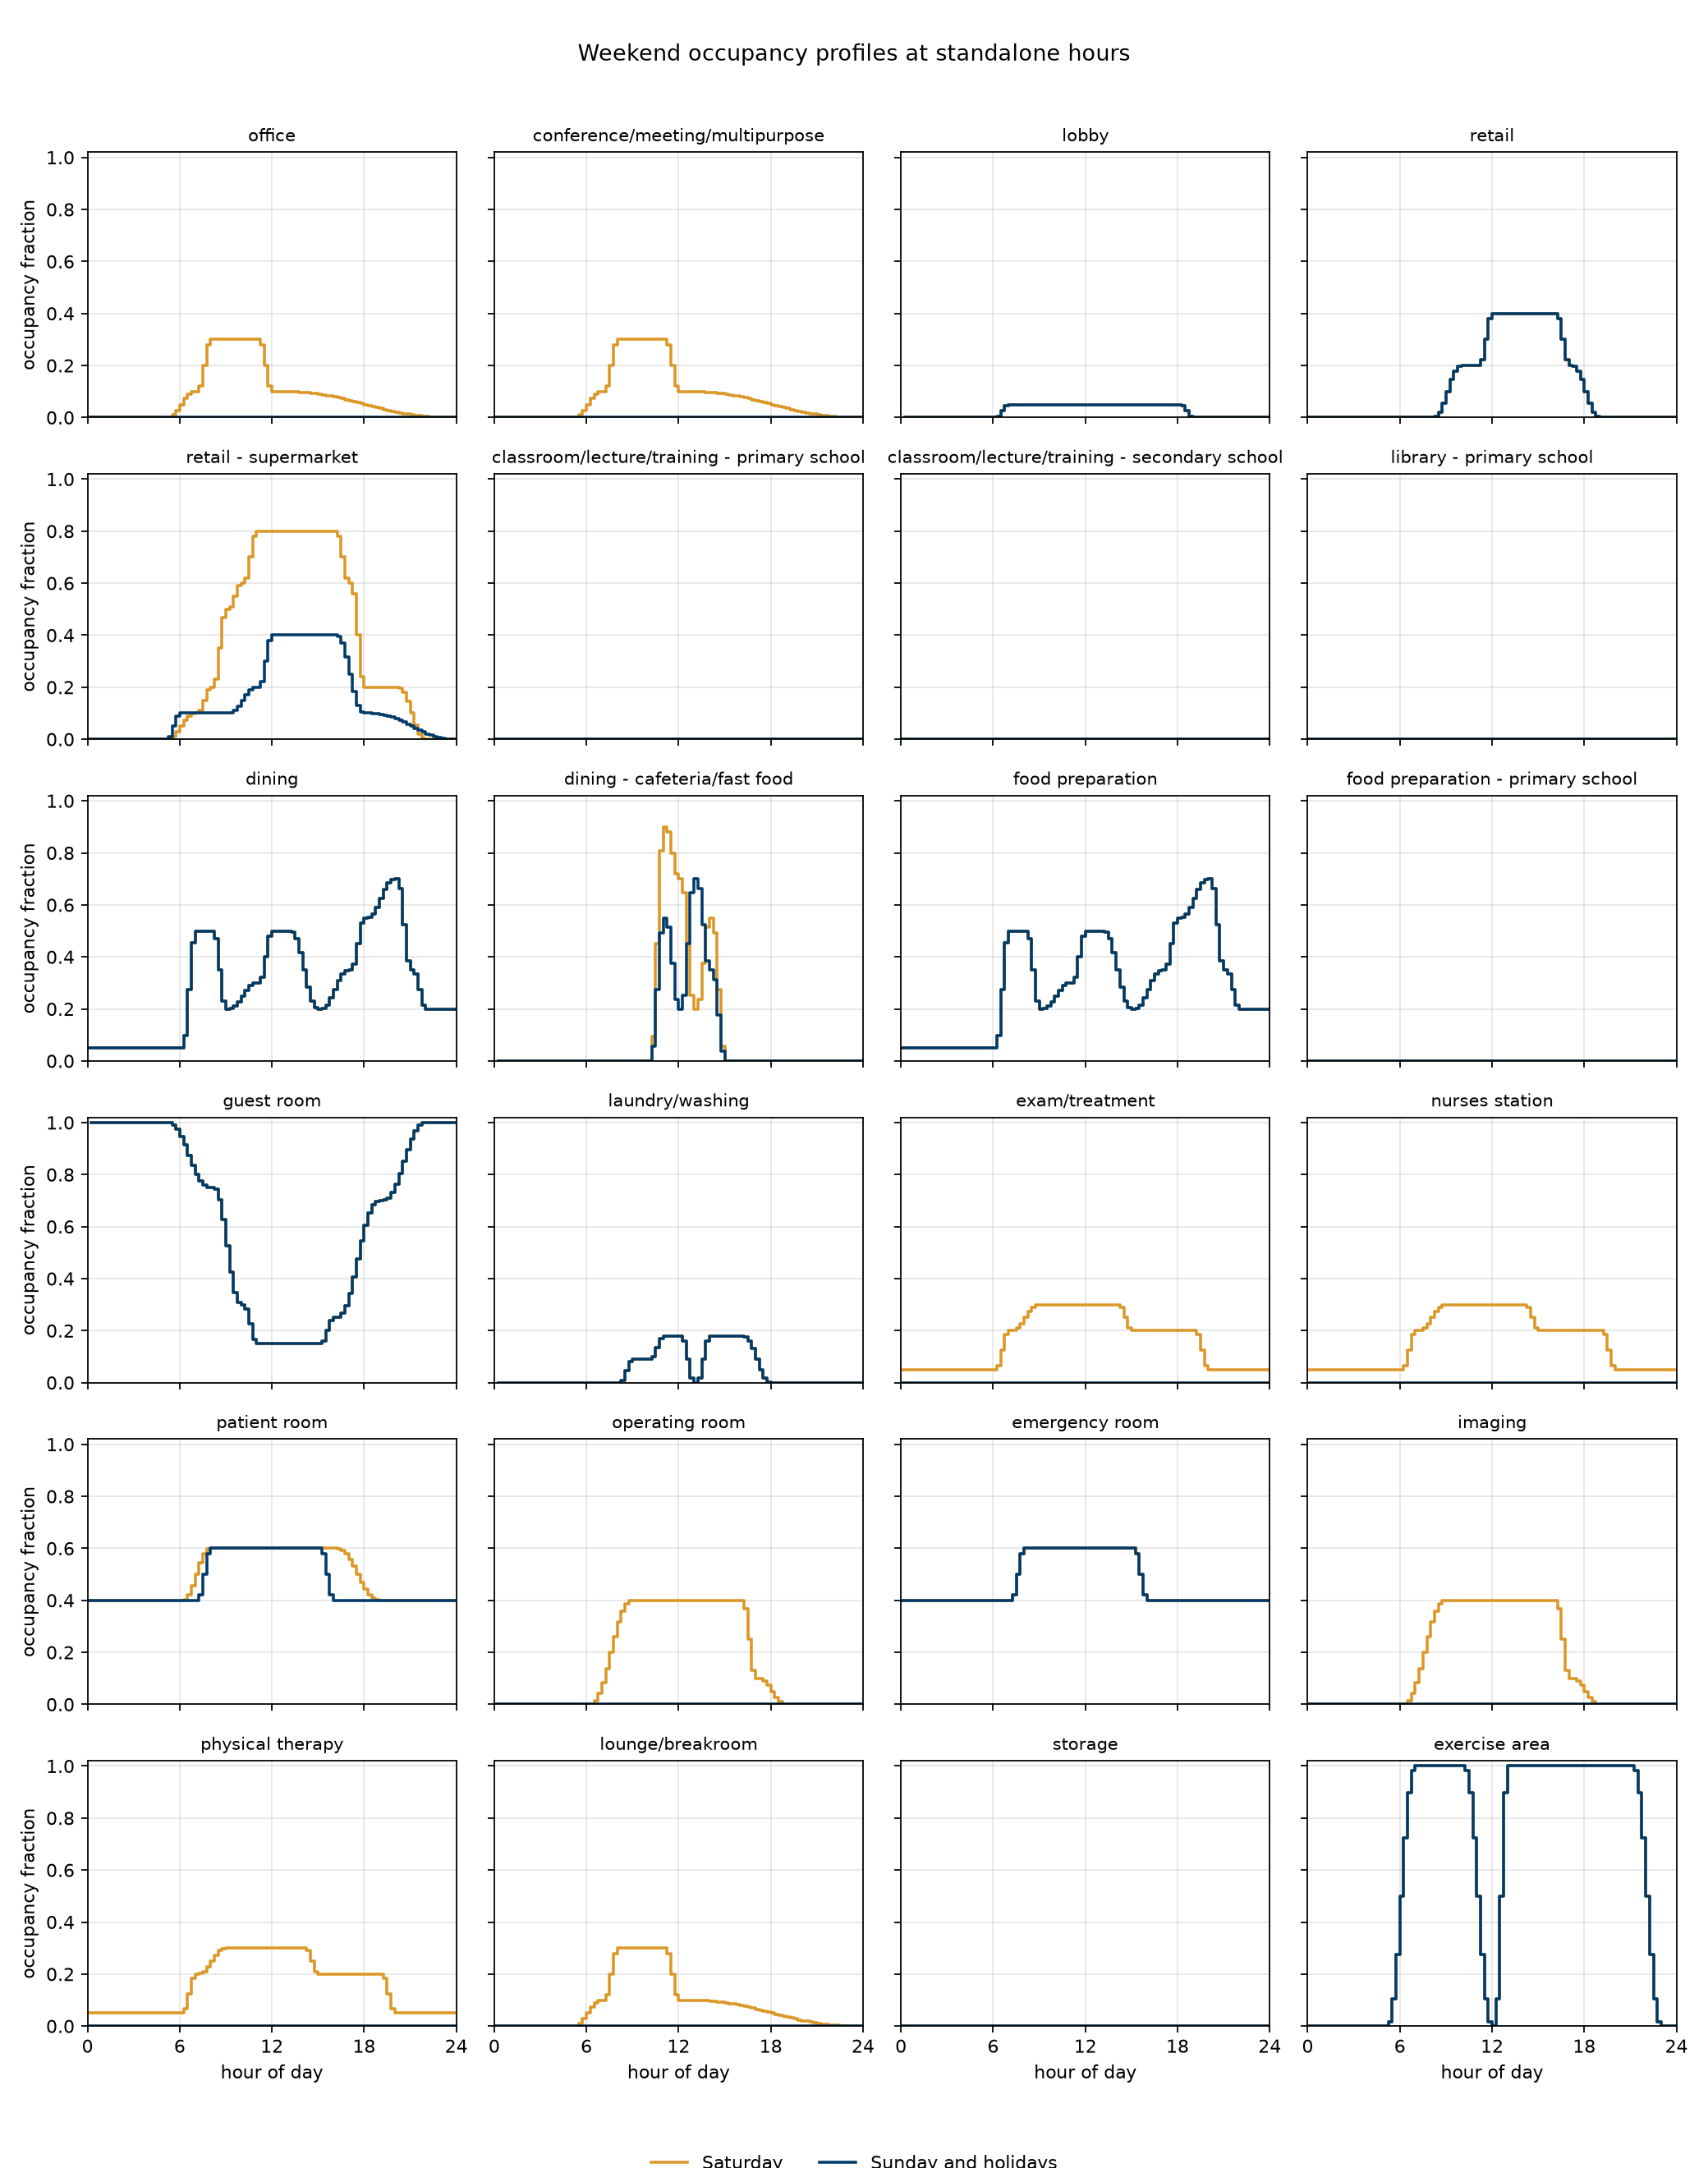
\includegraphics[width=1\textwidth]{figures/parametric_occupancy_weekend.png}
    \caption[Parametric weekend occupancy profiles]{Weekend occupancy profiles of the space types in Figures~\ref{fig:parametric_occupancy_1} and~\ref{fig:parametric_occupancy_2}, expanded at each schedule's standalone weekend start and end times. Saturday and Sunday profiles are shown where a space type carries both.}
    \label{fig:parametric_occupancy_weekend}
\end{figure}


% \begin{figure}
%   \centering
%   \includegraphics[scale=0.5]{figures/cbecs_comstock_fuel_comparison_full_service_restaurant.png}
%   \caption[Comparison of fuel type prevalence between ComStock and CBECS for full service restaurants]{Area-weighted vs. building-count-weighted comparison of fuel type prevalence between ComStock and CBECS for full service restaurants. From left to right, the fuel types on the x-axis are: district heating, electricity, fuel oil, natural gas, and propane.}
% \label{fig:cbecs_comstock_fuel_comparison_full_service_restaurant}
% \end{figure}

% \begin{figure}
%   \centering
%   \includegraphics[scale=0.5]{figures/cbecs_comstock_fuel_comparison_hospital.png}
%   \caption[Comparison of fuel type prevalence between ComStock and CBECS for hospitals]{Area-weighted vs. building-count-weighted comparison of fuel type prevalence between ComStock and CBECS for hospitals. From left to right, the fuel types on the x-axis are: district heating, electricity, fuel oil, natural gas, and propane.}
%   \label{fig:cbecs_comstock_fuel_comparison_hospital}
% \end{figure}

% \begin{figure}
%   \centering
%   \includegraphics[scale=0.5]{figures/cbecs_comstock_fuel_comparison_large_hotel.png}
%   \caption[Comparison of fuel type prevalence between ComStock and CBECS for large hotels]{Area-weighted vs. building-count-weighted comparison of fuel type prevalence between ComStock and CBECS for large hotels. From left to right, the fuel types on the x-axis are: district heating, electricity, fuel oil, natural gas, and propane.}
%   \label{fig:cbecs_comstock_fuel_comparison_large_hotel}
% \end{figure}

% \begin{figure}
%   \centering
%   \includegraphics[scale=0.5]{figures/cbecs_comstock_fuel_comparison_large_office.png}
%   \caption[Comparison of fuel type prevalence between ComStock and CBECS for large offices]{Area-weighted vs. building-count-weighted comparison of fuel type prevalence between ComStock and CBECS for large offices. From left to right, the fuel types on the x-axis are: district heating, electricity, fuel oil, natural gas, and propane.}
%   \label{fig:cbecs_comstock_fuel_comparison_large_office}
% \end{figure}

% \begin{figure}
%   \centering
%   \includegraphics[scale=0.5]{figures/cbecs_comstock_fuel_comparison_medium_office.png}
%   \caption[Comparison of fuel type prevalence between ComStock and CBECS for medium offices]{Area-weighted vs. building-count-weighted comparison of fuel type prevalence between ComStock and CBECS for medium offices. From left to right, the fuel types on the x-axis are: district heating, electricity, fuel oil, natural gas, and propane.}
%   \label{fig:cbecs_comstock_fuel_comparison_medium_office}
% \end{figure}

% \begin{figure}
%   \centering
%   \includegraphics[scale=0.5]{figures/cbecs_comstock_fuel_comparison_outpatient.png}
%   \caption[Comparison of fuel type prevalence between ComStock and CBECS for outpatient]{Area-weighted vs. building-count-weighted comparison of fuel type prevalence between ComStock and CBECS for outpatient. From left to right, the fuel types on the x-axis are: district heating, electricity, fuel oil, natural gas, and propane.}
%   \label{fig:cbecs_comstock_fuel_comparison_outpatient}
% \end{figure}

% \begin{figure}
%   \centering
%   \includegraphics[scale=0.5]{figures/cbecs_comstock_fuel_comparison_primary_school.png}
%   \caption[Comparison of fuel type prevalence between ComStock and CBECS for primary schools]{Area-weighted vs. building-count-weighted comparison of fuel type prevalence between ComStock and CBECS for primary schools. From left to right, the fuel types on the x-axis are: district heating, electricity, fuel oil, natural gas, and propane.}
%   \label{fig:cbecs_comstock_fuel_comparison_primary_school}
% \end{figure}

% \begin{figure}
%   \centering
%   \includegraphics[scale=0.5]{figures/cbecs_comstock_fuel_comparison_quick_service_restaurant.png}
%   \caption[Comparison of fuel type prevalence between ComStock and CBECS for quick service restaurants]{Area-weighted vs. building-count-weighted comparison of fuel type prevalence between ComStock and CBECS for quick service restaurants. From left to right, the fuel types on the x-axis are: district heating, electricity, fuel oil, natural gas, and propane.}
%   \label{fig:cbecs_comstock_fuel_comparison_quick_service_restaurant}
% \end{figure}

% \begin{figure}
%   \centering
%   \includegraphics[scale=0.5]{figures/cbecs_comstock_fuel_comparison_retail.png}
%   \caption[Comparison of fuel type prevalence between ComStock and CBECS for retail]{Area-weighted vs. building-count-weighted comparison of fuel type prevalence between ComStock and CBECS for retail. From left to right, the fuel types on the x-axis are: district heating, electricity, fuel oil, natural gas, and propane.}
%   \label{fig:cbecs_comstock_fuel_comparison_retail}
% \end{figure}

% \begin{figure}
%   \centering
%   \includegraphics[scale=0.5]{figures/cbecs_comstock_fuel_comparison_secondary_school.png}
%   \caption[Comparison of fuel type prevalence between ComStock and CBECS for secondary schools]{Area-weighted vs. building-count-weighted comparison of fuel type prevalence between ComStock and CBECS for secondary schools. From left to right, the fuel types on the x-axis are: district heating, electricity, fuel oil, natural gas, and propane.}
%   \label{fig:cbecs_comstock_fuel_comparison_secondary_school}
% \end{figure}

% \begin{figure}
%   \centering
%   \includegraphics[scale=0.5]{figures/cbecs_comstock_fuel_comparison_small_hotel.png}
%   \caption[Comparison of fuel type prevalence between ComStock and CBECS for small hotel]{Area-weighted vs. building-count-weighted comparison of fuel type prevalence between ComStock and CBECS for small hotel. From left to right, the fuel types on the x-axis are: district heating, electricity, fuel oil, natural gas, and propane.}
%   \label{fig:cbecs_comstock_fuel_comparison_small_hotel}
% \end{figure}

% \begin{figure}
%   \centering
%   \includegraphics[scale=0.5]{figures/cbecs_comstock_fuel_comparison_small_office.png}
%   \caption[Comparison of fuel type prevalence between ComStock and CBECS for small office]{Area-weighted vs. building-count-weighted comparison of fuel type prevalence between ComStock and CBECS for small office. From left to right, the fuel types on the x-axis are: district heating, electricity, fuel oil, natural gas, and propane.}
%   \label{fig:cbecs_comstock_fuel_comparison_small_office}
% \end{figure}

% \begin{figure}
%   \centering
%   \includegraphics[scale=0.5]{figures/cbecs_comstock_fuel_comparison_strip_mall.png}
%   \caption[Comparison of fuel type prevalence between ComStock and CBECS for strip malls]{Area-weighted vs. building-count-weighted comparison of fuel type prevalence between ComStock and CBECS for strip malls. From left to right, the fuel types on the x-axis are: district heating, electricity, fuel oil, natural gas, and propane.}
%   \label{fig:cbecs_comstock_fuel_comparison_strip_mall}
% \end{figure}

% \begin{figure}
%   \centering
%   \includegraphics[scale=0.5]{figures/cbecs_comstock_fuel_comparison_warehouse.png}
%   \caption[Comparison of fuel type prevalence between ComStock and CBECS for warehouses]{Area-weighted vs. building-count-weighted comparison of fuel type prevalence between ComStock and CBECS for warehouses. From left to right, the fuel types on the x-axis are: district heating, electricity, fuel oil, natural gas, and propane.}
%   \label{fig:cbecs_comstock_fuel_comparison_warehouse}
% \end{figure}

\begin{figure}
    \centering \includegraphics[width=1.0\textwidth]{figures/hvac_system_type_prevalance.png}
    \caption[HVAC system type prevalence in all building types]{Prevalence of ComStock HVAC system types by total stock floor area; all building types.}
    \label{fig:hvac_sys_type_prevalence}
\end{figure}

\begin{figure}
    \centering \includegraphics[width=1.0\textwidth]{figures/HVAC_SYS_Type_PREV_FSR.png}
    \caption[HVAC system type prevalence in full service restaurants]{Prevalence of ComStock HVAC system types by total stock floor area; full service restaurants.}
    \label{fig:hvac_sys_type_prevalence_fsr}
\end{figure}

\begin{figure}
    \centering \includegraphics[width=1.0\textwidth]{figures/HVAC_SYS_Type_PREV_HOS.png}
    \caption[HVAC system type prevalence in hospitals]{Prevalence of ComStock HVAC system types by total stock floor area; hospitals.}
    \label{fig:hvac_sys_type_prevalence_hos}
\end{figure}

\begin{figure}
  \centering \includegraphics[width=1.0\textwidth]{figures/HVAC_SYS_Type_PREV_LrgHotel.png}
  \caption[HVAC system type prevalence in large hotels]{Prevalence of ComStock HVAC system types by total stock floor area; large hotels.}
  \label{fig:HVAC_SYS_Type_PREV_LrgHotel}
\end{figure}

\begin{figure}
    \centering \includegraphics[width=1.0\textwidth]{figures/HVAC_SYS_Type_PREV_LrgOffice.png}
    \caption[HVAC system type prevalence in large offices]{Prevalence of ComStock HVAC system types by total stock floor area; large offices.}
    \label{fig:hvac_sys_type_prevalence_lrgoffice}
\end{figure}

\begin{figure}
    \centering \includegraphics[width=1.0\textwidth]{figures/HVAC_SYS_Type_PREV_MedOffice.png}
    \caption[HVAC system type prevalence in medium offices]{Prevalence of ComStock HVAC system types by total stock floor area; medium offices.}
    \label{fig:hvac_sys_type_prevalence_medoffice}
\end{figure}

\begin{figure}
    \centering \includegraphics[width=1.0\textwidth]{figures/HVAC_SYS_Type_PREV_Outpatient.png}
    \caption[HVAC system type prevalence in outpatient]{Prevalence of ComStock HVAC system types by total stock floor area; outpatient.}
    \label{fig:hvac_sys_type_prevalence_outpatient}
\end{figure}

\begin{figure}
    \centering \includegraphics[width=1.0\textwidth]{figures/HVAC_SYS_Type_PREV_Primary_School.png}
    \caption[HVAC system type prevalence in primary schools]{Prevalence of ComStock HVAC system types by total stock floor area; primary schools.}
    \label{fig:hvac_sys_type_prevalence_primary_school}
\end{figure}

\begin{figure}
    \centering \includegraphics[width=1.0\textwidth]{figures/HVAC_SYS_Type_PREV_QSR.png}
    \caption[HVAC system type prevalence in quick service restaurants]{Prevalence of ComStock HVAC system types by total stock floor area; quick service restaurants.}
    \label{fig:hvac_sys_type_prevalence_qsr}
\end{figure}

\begin{figure}
    \centering \includegraphics[width=1.0\textwidth]{figures/HVAC_SYS_Type_PREV_Retail_Stripmall.png}
    \caption[HVAC system type prevalence in strip malls]{Prevalence of ComStock HVAC system types by total stock floor area; strip malls.}
    \label{fig:hvac_sys_type_prevalence_retail_strip_mall}
\end{figure}

\begin{figure}
    \centering \includegraphics[width=1.0\textwidth]{figures/HVAC_SYS_Type_PREV_Retail.png}
    \caption[HVAC system type prevalence in retail]{Prevalence of ComStock HVAC system types by total stock floor area; retail.}
    \label{fig:hvac_sys_type_prevalence_retail}
\end{figure}

\begin{figure}
    \centering \includegraphics[width=1.0\textwidth]{figures/HVAC_SYS_Type_PREV_Secondary_School.png}
    \caption[HVAC system type prevalence in secondary schools]{Prevalence of ComStock HVAC system types by total stock floor area; secondary schools.}
    \label{fig:hvac_sys_type_prevalence_secondary_school}
\end{figure}

\begin{figure}
    \centering \includegraphics[width=1.0\textwidth]{figures/HVAC_SYS_Type_PREV_Small_Hotel.png}
    \caption[HVAC system type prevalence in small hotels]{Prevalence of ComStock HVAC system types by total stock floor area; small hotels.}
    \label{fig:hvac_sys_type_prevalence_small_hotel}
\end{figure}

\begin{figure}
    \centering \includegraphics[width=1.0\textwidth]{figures/HVAC_SYS_Type_PREV_Small_Office.png}
    \caption[HVAC system type prevalence in small offices]{Prevalence of ComStock HVAC system types by total stock floor area; small offices.}
    \label{fig:hvac_sys_type_prevalence_small_office}
\end{figure}

\begin{figure}
    \centering \includegraphics[width=1.0\textwidth]{figures/HVAC_SYS_Type_PREV_Warehouse.png}
    \caption[HVAC system type prevalence in warehouses]{Prevalence of ComStock HVAC system types by total stock floor area; warehouses.}
    \label{fig:hvac_sys_type_prevalence_warehouse}
\end{figure}

\begin{figure}
    \centering \includegraphics[width=1.0\textwidth]{figures/cbecs_therm_summary.png}
    \caption[Percentage of buildings with thermostat setbacks from the CBECS 2012 survey]{Percentage of buildings with thermostat setbacks by building type from the CBECS 2012 survey.}
    \label{fig:cbecs_therm_setback_summary}
\end{figure}

\begin{figure}
    \centering \includegraphics[width=1.0\textwidth]{figures/All_Building_Types_thermostat_scatter.png}
    \caption[Correlation between thermostat set point and thermostat setback from BAS data]{Thermostat heating and cooling set point-setback delta correlation from BAS data sources; all building types.}
    \label{fig:therm_setpoint_setback}
\end{figure}

\pagebreak

\begin{figure}
    \centering \includegraphics[width=1.0\textwidth]{figures/boiler_performance_curves.png}
    \caption[Boiler part load performance curves]{Boiler part load performance curves.}
    \label{fig:blr_plr_curves}
\end{figure}


\begin{figure}
    \centering \includegraphics[width=1.0\textwidth]{figures/EIRFPLR.png}
    \caption[DX cooling energy input ratio as a function of part load ratio performance curves]{DX cooling energy input ratio as a function of part load ratio performance curves.}
    \label{fig:dx_eirfplr}
\end{figure}

\begin{figure}
    \centering \includegraphics[width=1.0\textwidth]{figures/CAPFF.png}
    \caption[DX cooling capacity as a function of airflow performance curves]{DX cooling capacity as a function of airflow performance curves.}
    \label{fig:dx_capff}
\end{figure}

\begin{figure}
    \centering \includegraphics[width=1.0\textwidth]{figures/EIRFF.png}
    \caption[DX cooling energy input ratio as a function of airflow performance curves]{DX cooling energy input ratio as a function of airflow performance curves.}
    \label{fig:dx_eirff}
\end{figure}

\begin{figure}
    \centering \includegraphics[width=1.0\textwidth]{figures/EIRFT.png}
    \caption[DX cooling energy input ratio as a function of temperature performance curves]{DX cooling energy input ratio as a function of temperature performance curves. Independent variables are outdoor air dry bulb temperature (y-axis, degrees Celsius) and wet bulb temperature entering the cooling coil (x-axis, degrees Celsius).}
    \label{fig:dx_eirft}
\end{figure}

\begin{figure}
    \centering \includegraphics[width=1.0\textwidth]{figures/CAPFT.png}
    \caption[DX cooling capacity as a function of temperature performance curves]{DX cooling capacity as a function of temperature performance curves. Independent variables are outdoor air dry bulb temperature (y-axis, degrees Celsius) and wet bulb temperature entering the cooling coil (x-axis, degrees Celsius).}
    \label{fig:dx_capft}
\end{figure}

\begin{figure}
    \centering \includegraphics[width=1.0\textwidth]{figures/ashp_eirft.png}
    \caption[Air-source heat pump COP ratio as a function of outdoor air dry bulb temperature]{Air-source heat pump COP ratio as a function of outdoor air dry bulb temperature.}
    \label{fig:ashp_eirft}
\end{figure}

\begin{figure}
    \centering \includegraphics[width=1.0\textwidth]{figures/ashp_eirfplr.png}
    \caption[Air-source heat pump EIR ratio as a function of part load ratio]{Air-source heat pump EIR ratio as a function of part load ratio.}
    \label{fig:ashp_eirfplr}
\end{figure}

\begin{figure}
    \centering \includegraphics[width=1.0\textwidth]{figures/ashp_eirff.png}
    \caption[Air-source heat pump EIR ratio as a function of airflow fraction]{Air-source heat pump EIR ratio as a function of airflow fraction.}
    \label{fig:ashp_eirff}
\end{figure}

\begin{figure}
    \centering \includegraphics[width=1.0\textwidth]{figures/ashp_capft.png}
    \caption[Air-source heat pump capacity as a function of outdoor air dry bulb temperature]{Air-source heat pump capacity as a function of outdoor air dry bulb temperature.}
    \label{fig:ashp_capft}
\end{figure}

\begin{figure}
    \centering \includegraphics[width=1.0\textwidth]{figures/ashp_capff.png}
    \caption[Air-source heat pump capacity as a function of airflow ratio]{Air-source heat pump capacity as a function of airflow ratio.}
    \label{fig:ashp_capff}
\end{figure}

\begin{figure}
    \centering \includegraphics[width=1.0\textwidth]{figures/ac_chiller_eir_curves.png}
    \caption[Air-cooled chiller EIR as a function of part load ratio performance curves]{Air-cooled chiller EIR as a function of part load ratio performance curves. Independent variables beyond the curve limits will use the bound of the curve limit during simulation.}
    \label{fig:acc_eir_curves}
\end{figure}

\begin{figure}
    \centering \includegraphics[width=1.0\textwidth]{figures/AirCooled_Chiller_2010_PathA_Modifiers.png}
    \caption["AirCooledChiller2010PathA" modifier performance curves]{``AirCooledChiller2010PathA'' modifier performance curves; capacity as a function of temperature and EIR as a function of temperature. Independent variables beyond the curve limits will use the bound of the curve limit during simulation.}
    \label{fig:AirCooledChiller2010PathA_funct_curves}
\end{figure}

\begin{figure}
    \centering \includegraphics[width=1.0\textwidth]{figures/ChlrAirRecipQRatio_Modifiers.png}
    \caption["ChlrAirRecip" modifier performance curves]{``ChlrAirRecip'' modifier performance curves; capacity as a function of temperature and EIR as a function of temperature. Independent variables beyond the curve limits will use the bound of the curve limit during simulation.}
    \label{fig:ChlrAirRecipQRatio_curves}
\end{figure}

\begin{figure}
    \centering \includegraphics[width=1.0\textwidth]{figures/wcc_plr.png}
    \caption{Energy input ratio modifier as a function of water-cooled chiller part load ratio.}
    \label{fig:wcc_plr}
\end{figure}

\begin{figure}
    \centering \includegraphics[width=1.0\textwidth]{figures/WaterCooled_PositiveDisplacement_Chiller_LT150_2010_Modifiers.png}
    \caption[Performance curves for WCC]{Performance curves for ``WaterCooled PositiveDisplacement Chiller LT150 2010 Modifiers'' WCC.}
    \label{fig:wcc_WaterCooled_PositiveDisplacement_Chiller_LT150_2010_Modifiers}
\end{figure}

\begin{figure}
    \centering \includegraphics[width=1.0\textwidth]{figures/ChlrWtrPosDispPathAAll_Modifiers.png}
    \caption{Performance curves for ``ChlrWtrPosDispPathAAll Modifiers'' WCC.}
    \label{fig:wcc_ChlrWtrPosDispPathAAll_Modifiers}
\end{figure}

\begin{figure}
    \centering \includegraphics[width=1.0\textwidth]{figures/ground_loop_outlet_temperatures.png}
    \caption{Ground loop outlet vs. inlet temperature relationship for GSHPs.}
    \label{fig:gshp_loop_temps}
\end{figure}


\begin{figure}
    \centering \includegraphics[width=1.0\textwidth]{figures/refrigeration_MTold.png}
    \caption[Compressor performance for small, old, medium temperature compressors]{Power and capacity values as a function of suction and discharge temperature for small, old, medium-temperature compressors.}
    \label{fig:refrig_mt_old}
\end{figure}

\begin{figure}
    \centering \includegraphics[width=1.0\textwidth]{figures/refrigeration_MTnew.png}
    \caption[Compressor performance for large, new, medium temperature compressors]{Power and capacity values as a function of suction and discharge temperature for large, new, medium-temperature compressors.}
    \label{fig:refrig_mt_new}
\end{figure}

\begin{figure}
    \centering \includegraphics[width=1.0\textwidth]{figures/refrigeration_LTold.png}
    \caption[Compressor performance for small, old, low temperature compressors]{Power and capacity values as a function of suction and discharge temperature for small, old, low-temperature compressors.}
    \label{fig:refrig_lt_old}
\end{figure}

\begin{figure}
    \centering \includegraphics[width=1.0\textwidth]{figures/refrigeration_LTnew.png}
    \caption[Compressor performance for large, new, low temperature compressors]{Power and capacity values as a function of suction and discharge temperature for large, new, low-temperature compressors.}
    \label{fig:refrig_lt_new}
\end{figure}

\begin{figure} [ht!]
    \includegraphics[width=0.8\textwidth]{figures/soil_conductivity.png}
    \centering
    \caption[Soil thermal conductivity distributions by climate zone]{Soil thermal conductivity distributions by climate zone.}
    \label{fig:soil_conductivity}
\end{figure}
  

\end{appendices}

\end{document}
